%!TEX TS-program = xelatex
\documentclass[10pt,table,a4]{article}\usepackage[]{graphicx}\usepackage[]{color}

\usepackage{alltt}
\usepackage{graphicx}
\usepackage{gensymb}
\usepackage[top=1cm, bottom=1.5cm, left=1.2cm, right=1.2cm]{geometry}
\usepackage[font=small]{caption}
\usepackage{adjustbox}
\usepackage{fancyhdr}
\usepackage{layout}
%\usepackage{booktabs}
%\usepackage{kpfonts}
\usepackage[explicit]{titlesec}
\usepackage{wrapfig}
\usepackage{tcolorbox}
\usepackage{xcolor}
\usepackage{setspace}
\usepackage{parskip}
\usepackage{tikz}
\usepackage{fontspec}
\usepackage{anyfontsize}
\usepackage{hyperref}
\usepackage{multicol}
\usepackage{datetime}
\usepackage{fixltx2e}
\usepackage{mfirstuc}
\usepackage[sfdefault]{ClearSans}

% Colours
\definecolor{Yellow1}{RGB}{252, 190, 14}
\definecolor{Yellow2}{RGB}{252, 190, 54}
\definecolor{Yellow3}{RGB}{254, 238, 207}

\definecolor{OffBlack}{RGB}{61,61,60}
\definecolor{LightGray}{RGB}{208,208,208}

\definecolor{ColRed}{RGB}{244,123,115}
\definecolor{ColOrange}{RGB}{253,226,145}
\definecolor{ColYellow}{RGB}{255,255,204}
\definecolor{ColGreen}{RGB}{195,214,155}

\pagestyle{fancy}
\fancyhf{}
%\fancyhead[R]{\thepage}
\renewcommand{\headrulewidth}{0pt}

\newcolumntype{P}[1]{>{\centering\arraybackslash}p{#1}}


\newcommand{\nearr}[1]{$\color{#1}\nearrow$}
\newcommand{\searr}[1]{$\color{#1}\searrow$}
\newcommand{\uparr}[1]{$\color{#1}\uparrow$}




\setlength{\parskip}{10pt}

%\pagenumbering{gobble}

\newcommand*{\PageHeadingSingleLine}{%
	\begin{tikzpicture}[remember picture,overlay]
	\node[anchor=north west,minimum width=.375cm,minimum height=1.2cm,fill=Yellow1] (RB) at (-1.2,1.2){\Large };
	%\node[text=OffBlack, right of=RB, xshift = 18cm, yshift=0.75cm] at (0,0){\thepage};
	\end{tikzpicture}}
\newcommand*{\PageHeadingDoubleLine}{%
	\begin{tikzpicture}[remember picture, overlay]
	\node[anchor=north west,minimum width=.375cm,minimum height=1.9cm,fill=Yellow1] (RB) at (-1.2,1.2){\Large };
	%\node[text=OffBlack, right of=RB, xshift = 18cm, yshift=0.6cm] at (0,0){\thepage};
	\end{tikzpicture}}
\newcommand{\HeaderSingle}[1]{
	\PageHeadingSingleLine 
	
	\vspace{-1.2cm}
	{\Large\textbf{#1}}
	\vspace{.2cm}}
\newcommand{\HeaderDouble}[2]{
	\PageHeadingDoubleLine
	
	\vspace{-1.2cm}
	{\Large\textbf{#1 \\[10pt] #2}}
	\vspace{.45cm}}
\newcommand*{\SectionHeadingBox}[1]{%
	\begin{tikzpicture}[remember picture, overlay]
	\node[anchor=north west,minimum width=.375cm,minimum height=#1,fill=Yellow1] (RB) at (-1.2,-16){\Large };
	\end{tikzpicture}
	\vspace{.8cm}}
\newcommand{\SectionHeading}[2]{
	\SectionHeadingBox{3cm}
	
	\vspace{15.7cm}
	\textbf{{\Huge #1 \\[6pt]\Huge #2}}}
\newcommand{\SectionHeadingDouble}[3]{
	\SectionHeadingBox{4cm}
	
	\vspace{15.7cm}
	\textbf{{\Huge #1 \\[6pt]\Huge #2\\[6pt]\Huge #3}}}
\newcommand{\PageFooterFirst}{% The number indicates the sector..... 
	\begin{tikzpicture}[remember picture, overlay]
	\node[text=OffBlack,above = .8cm, left = 6cm,font=\bf\small,align=center] at (current page.south){01-INTRODUCTION};
	\node[text=LightGray,above = .8cm, left = 1.7cm,font=\bf\small,align=center] at (current page.south){02-CURRENT EXPOSURE};
	\node[text=LightGray,above = .8cm, left = -1cm,font=\bf\small,align=center] at (current page.south){03-5YR TREND};
	\node[text=LightGray,above = .8cm, left = -5cm,font=\bf\small,align=center] at (current page.south){04-EXPOSURE IN 5YRS};
	\node[text=LightGray,above = .8cm, left = -9cm,font=\bf\small,align=center] at (current page.south){05-COMPANY RESULTS};	
	\node[left=6cm,minimum width = 3.0cm, minimum height =0.01cm, fill = Yellow1] at (current page.south){};
	\end{tikzpicture}
}
\newcommand{\PageFooterSecond}{% The number indicates the sector..... 
	\begin{tikzpicture}[remember picture, overlay]
	\node[text=LightGray,above = .8cm, left = 6cm,font=\bf\small,align=center] at (current page.south){01-INTRODUCTION};
	\node[text=OffBlack,above = .8cm, left = 1.7cm,font=\bf\small,align=center] at (current page.south){02-CURRENT EXPOSURE};
	\node[text=LightGray,above = .8cm, left = -1cm,font=\bf\small,align=center] at (current page.south){03-5YR TREND};
	\node[text=LightGray,above = .8cm, left = -5cm,font=\bf\small,align=center] at (current page.south){04-EXPOSURE IN 5YRS};
	\node[text=LightGray,above = .8cm, left = -9cm,font=\bf\small,align=center] at (current page.south){05-COMPANY RESULTS};	
	\node[left=1.75cm,minimum width = 3.6cm, minimum height =0.01cm, fill = Yellow1] at (current page.south){};
	\end{tikzpicture}
}
\newcommand{\PageFooterThird}{% The number indicates the sector..... 
	\begin{tikzpicture}[remember picture, overlay]
	\node[text=LightGray,above = .8cm, left = 6cm,font=\bf\small,align=center] at (current page.south){01-INTRODUCTION};
	\node[text=LightGray,above = .8cm, left = 1.7cm,font=\bf\small,align=center] at (current page.south){02-CURRENT EXPOSURE};
	\node[text=OffBlack,above = .8cm, left = -1cm,font=\bf\small,align=center] at (current page.south){03-5YR TREND};
	\node[text=LightGray,above = .8cm, left = -5cm,font=\bf\small,align=center] at (current page.south){04-EXPOSURE IN 5YRS};
	\node[text=LightGray,above = .8cm, left = -9cm,font=\bf\small,align=center] at (current page.south){05-COMPANY RESULTS};	
	\node[left=-.9cm,minimum width = 2.2cm, minimum height =0.01cm, fill = Yellow1] at (current page.south){};
	\end{tikzpicture}
}
\newcommand{\PageFooterFourth}{% The number indicates the sector..... 
	\begin{tikzpicture}[remember picture, overlay]
	\node[text=LightGray,above = .8cm, left = 6cm,font=\bf\small,align=center] at (current page.south){01-INTRODUCTION};
	\node[text=LightGray,above = .8cm, left = 1.7cm,font=\bf\small,align=center] at (current page.south){02-CURRENT EXPOSURE};
	\node[text=LightGray,above = .8cm, left = -1cm,font=\bf\small,align=center] at (current page.south){03-5YR TREND};
	\node[text=OffBlack,above = .8cm, left = -5cm,font=\bf\small,align=center] at (current page.south){04-EXPOSURE IN 5YRS};
	\node[text=LightGray,above = .8cm, left = -9cm,font=\bf\small,align=center] at (current page.south){05-COMPANY RESULTS};	
	\node[left=-5cm,minimum width = 3.5cm, minimum height =0.01cm, fill = Yellow1] at (current page.south){};
	\end{tikzpicture}
}
\newcommand{\PageFooterFifth}{% The number indicates the sector..... 
	\begin{tikzpicture}[remember picture, overlay]
	\node[text=LightGray,above = .8cm, left = 6cm,font=\bf\small,align=center] at (current page.south){01-INTRODUCTION};
	\node[text=LightGray,above = .8cm, left = 1.7cm,font=\bf\small,align=center] at (current page.south){02-CURRENT EXPOSURE};
	\node[text=LightGray,above = .8cm, left = -1cm,font=\bf\small,align=center] at (current page.south){03-5YR TREND};
	\node[text=LightGray,above = .8cm, left = -5cm,font=\bf\small,align=center] at (current page.south){04-EXPOSURE IN 5YRS};
	\node[text=OffBlack,above = .8cm, left = -9cm,font=\bf\small,align=center] at (current page.south){05-COMPANY RESULTS};	
	\node[left=-8.9cm,minimum width = 3.4cm, minimum height =0.01cm, fill = Yellow1] at (current page.south){};
	\end{tikzpicture}
}

\setmainfont{ClearSans}
\color{OffBlack}


\newcommand\mypage{\textcolor{OffBlack}{\large\thepage}}
\newcommand{\PageFooter}[1]{% The number indicates the sector..... 
	\begin{tikzpicture}[remember picture, overlay]
	\node[text=OffBlack,above = 1.2cm, left = -9.43cm,font=\bf\small,align=center] at (current page.south){ #1 \textcolor{Yellow1}{\textbf{|}} \thepage};	
	\end{tikzpicture}
}

% Box with a shaded border
\newtcolorbox{shadedbox}{colback=Yellow3}

\begin{document}
	\section*{} % Front Page
	
	
	\thispagestyle{empty}
	\pagecolor{Yellow1}
	
	\vspace{-2.6cm}
	
	\begin{tikzpicture}[remember picture, overlay]
	\vspace{7cm}
	\node[below=-.6cm] (CN) at (current page.north){\adjincludegraphics[height=15cm,trim={0cm 0cm 0cm 2cm},clip]{ReportGraphics/FrontPageUNPRI.jpg}
	};
	
	\node[below = 4.5cm, right,align = left, white, text width=10cm](TN) at (current page.center){
		\Huge{\textbf{SCENARIO ANALYSIS}}\\[10pt]
		{\baselineskip=20pt\LARGE\raggedright{\textbf{scenarioName}\par}}
		\vspace{1cm}
		{\baselineskip=20pt\Huge\raggedright{\textbf{InvestorName}\par}}
		\vspace{.4cm}
		{\baselineskip=20pt\LARGE\raggedright{\textbf{PortfolioName}\par}}};
	
	\node[below = 4.4cm,right= .12cm, minimum width = 3cm, minimum height =0.05cm,fill= OffBlack] at (current page.center){};
	
	\end{tikzpicture}
	
	
	\begin{tikzpicture}[remember picture,overlay]
	\node[anchor=south west, yshift = 0cm ,minimum width=21.6cm,minimum height=4cm,fill=white] (RB) at (current page.south west){};
	\node[left= 7cm, above=1.cm] (WS) at (current page.south){\adjincludegraphics[height=1.8cm,trim={0cm 0cm 0cm 0cm},clip]{ReportGraphics/Logo_front}};
	\node[ below = 1.8cm, minimum width = 3.5cm, minimum height =0.05cm, fill = Yellow1] at (WS){};
	\end{tikzpicture}
	
	
	
	
	
	\newpage
	\pagecolor{white}
	
	\begin{center}
		\textbf{2Dii PACTA MODEL}
		
		\textbf{Important Information \& Legal Disclaimer: MODEL OUTPUT REPORTS}
		
		\textbf{IMPORTANT INFORMATION}
		
	\end{center}
	
	
	The 2Dii PACTA Model generates a limited 'point in time' estimate of the relative alignment of the Revealed Plans of Securities in the Scope versus the economic trends embodied in the Scenario(s), as identified by external data and scenario providers. 
	
	\textbf{EXCLUSION OF LIABILITY: }TO THE EXTENT PERMITTED BY LAW WE WILL NOT BE LIABLE TO ANY USER FOR ANY LOSS OR DAMAGE, WHETHER IN CONTRACT, TORT (INCLUDING NEGLIGENCE), BREACH OF STATUTORY DUTY OR OTHERWISE, EVEN IF FORESEEABLE, ARISING UNDER OR IN CONNECTION WITH USE OF OR RELIANCE ON ANY INFORMATION, DATA OR CONTENT OBTAINED VIA OUR SERVICES, INCLUDING (WITHOUT LIMITATION) THE MODELLING OUTPUTS STATED IN THIS REPORT.
	
	\textbf{No forecast or prediction: }The PACTA Model does not purport to generate, nor does this Report contain or comprise, statements of fact, forecasts or predictions. The PACTA Model provides a 'point in time' analysis of economic and commercial variables that are inherently dynamic and variable over time. 2Dii neither makes nor implies any representation regarding the likelihood, risk or expectation of any future matter. To the extent that any statements made or information contained in this Report might be considered forward-looking in nature, they are subject to risks, variables and uncertainties that could cause actual results to differ materially. You are cautioned not to place undue reliance on any such forward-looking statements, which reflect our assumptions only and those of our data and scenario providers as of the date of modelling.
	
	\textbf{No financial advice: }The information contained in this Report does not comprise, constitute or provide, nor should it be relied upon as, investment or financial advice, credit ratings, an advertisement, an invitation, a confirmation, an offer or a solicitation, or recommendation, to buy or sell any security or other financial, credit or lending product or to engage in any investment activity, or an offer of any financial service. This Report does not purport to quantify risk to the portfolio (or any part thereof), nor make any representation in regards to the performance, strategy, prospects, creditworthiness or risk associated with any investment, nor their suitability for purchase, holding or sale in the context of any particular portfolio. The Modelling Outputs reflected in this Report are provided with the understanding and expectation that each investor will, with due care, conduct its own investigation and evaluation of each security or other instrument that is under consideration for purchase, holding or sale. 
	
	\textbf{Scope Securities: }The PACTA Model is limited in its scope and application. It does not consider all securities across all sectors, nor all securities within those sectors. The PACTA Model applies only to the Scope Securities set out in the Methodology Statement, as updated from time to time. 
	
	\textbf{Scenario(s): }The PACTA Model will apply one or more Scenarios, as set out in the Methodology Statement. The choice of any Scenario should not be taken as any endorsement of those scenarios, nor any statement as to the accuracy or completeness of those scenarios' methodologies or assumptions, nor as a general preference of those scenarios over any other economic scenarios. The analysis provided by the PACTA Model may be carried out using other economic scenarios, and users must form their own view as to the decarbonisation scenarios, trajectories and models that are most appropriate to their portfolio. No explicit or implicit assumption is made in relation to the current or future alignment of the Scenarios with climate-related policies of any government at international, national or sub-national level.
	
	\textbf{TCFD: }Use of the PACTA Modelling Tool may support you in initiatives undertaken with regard to the Recommendations of G20 Financial Stability Board's Taskforce on Climate-related Financial Disclosures (TCFD). However, its use in isolation does not purport to provide 'TCFD compliance'. 
	
	
	%UNPRI_TextS
	\textbf{PRI: }Please note that the PACTA climate scenario tool is made available by 2Dii and not PRI Association or any of its affiliated entities (``PRI"). PRI takes no responsibility for the performance and/or use of the tool and shall have no liability whatsoever whether arising in contract, tort (including negligence) or otherwise arising under or in connection with these terms and conditions, this website or any use of the PACTA climate scenario tool.
	%UNPRI_TextE	

	\newpage
	
	\section*{} % 1st Section
	\SectionHeading{SECTION 1:}{INTRODUCTION}
	
	
	\newpage
	\section*{} % Report Contents
	\HeaderSingle{REPORT CONTENTS}
	
	\begin{multicols}{2}
		
		\textbf{This report provides a scenario analysis, following part of the recommendations of the G20's Financial Stability Board Task Force on Climate-related Financial Disclosures (TCFD). Specifically, it seeks to inform the reader about four issues.}
		
		\begin{enumerate}
			\item{\textbf{What is the current exposure of the portfolio to economic activities affected by the transition to a low-carbon economy? (Section 2) }
			}
			
			The first part of the report summarizes the exposures of the portfolio (in terms of \% of the portfolio) to business activities potentially affected by the transition to a low-carbon economy and by extension to transition risk. Specifically, it will quantify the percent of the portfolio exposed to low-carbon and high-carbon activities across the fossil fuel, power, and automotive sectors. The results will be presented relative to the market.
			
			\item{\textbf{Does the portfolio increase or decrease its alignment to the ScenarioValue over the next 5 years? (Section 3)}
			}
			
			The second part of the report will quantify the extent to which the portfolio is building or reducing risk in terms of being aligned / misaligned with the ScenarioValue pathway over the next 5 years. The analysis will focus on technologies in the fossil fuel sector (oil production, gas production, coal mining), electric power sector (coal power, gas power, nuclear power, renewables power), and automotive sector (internal combustion engine vehicles and electric vehicles). Additionally, information is provided regarding the necessary progression of carbon emission intensity for the aviation, shipping, cement and steel sectors compared to Energy Technology Perspectives scenarios from the IEA. 
			
			\item{\textbf{What is the expected future exposure to high- and low-carbon economic activities based on the current revealed production and investment plans of the companies in the portfolio? (Section 4)}
			}
			
			Section 4 of this report will quantify the expected evolution of the portfolio's exposure to high-carbon and low-carbon activities in 5 years (Startyear+5) based on the current revealed production and investment plans of companies in portfolio with business activities in the fossil fuel, power, and automotive sectors. The section will show the portfolio's expected future technology mix in each sector compared to the expected future technology mix of both the aggregated investment portfolio of the peer group included in this analysis and the market aligned to a ScenarioValue. Additionally the regional exposure to coal mining activities shall also be displayed. 
			
			\item{\textbf{What is driving the results? (Section 5)}}
			
			Section 5 will provide background on the securities and companies driving the results presented in the previous sections, including additional analysis on individual companies' profiles. 
			
			\textit{For clarity, background information outlining the context of scenario analysis, the scenarios and modelling and transition risk is provided at the end of the report (Section 6).}
			%WWFSpecificIncludeS
			\textit{The views of WWF are also included in Section 6.}
			%WWFSpecificIncludeE
			
			
		\end{enumerate}
		
		
	\end{multicols}
	
	%	\vspace{1cm}
	\begin{tikzpicture}[remember picture, overlay]
	\node[anchor=north west,minimum width=.375cm,minimum height=5.2cm,fill=Yellow1] (ToC) at (-1.2,-.4){};
	\end{tikzpicture}	
	
	\begin{minipage}[t]{.5\linewidth}
		\textbf{Section 1: }Introduction\\
		
		\textbf{Section 2: }The current exposure\\
		
		\textbf{Section 3: }Trajectory of the portfolio relative to transition scenarios\\
		
		\textbf{Section 4: }The expected exposure in Startyear+5\\
		
		\textbf{Section 5: }Company exposure\\
		
		\textbf{Section 6: }Background to the model\\
	\end{minipage}
	
	%\PageFooterFirst
\PageFooter{1 - INTRODUCTION}
	\newpage
	
		\section*{} % Exec Summary p3
	\HeaderSingle{ANALYSIS SUMMARY}
	
	\begin{multicols}{2}
		\textbf{This report provides a scenario analysis of the investment portfolio.} 
		
		It responds in part to the recommendations of the G20 Financial Stability Board Task Force on Climate-related Financial Disclosures (TCFD). Over 1,500 financial institutions have been assessed using the model applied in this report, as part of direct partnerships with over 200 institutional investors, and collaborations with a number of financial supervisors and sector associations. 
		
		The outputs provided in this report provide an analysis of the portfolio relative to an economic transition consistent with limiting global warming to ScenarioTemp\degree C above pre-industrial levels, as well as a comparison to peers. The analysis provides answers to three questions: 
		
		\begin{enumerate}
			\item{What is the current exposure in the portfolio to economic activities affected by the transition to a low-carbon economy? (Section 2)}
			\item{Does the portfolio increase or decrease its alignment with a scenarioName transition over the next 5 years? (Section 3)}
			\item{What is the expected future exposure to high- and low-carbon economic activities? (Section 4)}
		\end{enumerate}
		
		This report considers a ScenarioValue transition. scenarioDescription The analysis covers two asset classes: listed equity and corporate bonds. These are compared to either a portfolio or market, as if they would transition aligned to the ScenarioValue. The equity market is represented by the MSCI ACWI index and the corporate bond market by the BEHGTRUU index. \columnbreak
		
		
		
		\begin{center}
			{\rowcolors{2}{white}{Yellow3}
				\setlength{\tabcolsep}{10pt} % Default value: 6pt
				\renewcommand{\arraystretch}{1.5} % Default value: 1
				\begin{tabular}{ p{.35\linewidth} p{.49\linewidth} }
					\hline
					\multicolumn{2}{c}{\textbf{Scope of Analysis}} \\
					\hline
					Investor Name & InvestorName \\ 
					Portfolio Name & PortfolioName \\ 
					Size of portfolio & SizeofPortfolio \\ 
					Scenario & ScenarioText \\ 
					Geography - \newline Financial Assets & Global \\ 
					Geography - \newline Economic Assets & Global \\ 
					Asset Class & AssetClass \\ 
					Peers & PeerGroup \\
					Portfolio Timestamp & ReportDate \\ 
					Date of Analysis & TodaysDate \\ 
					\hline
				\end{tabular}
			}
			
		\end{center}
		
		The analysis focuses on climate relevant sectors. Scenario analysis is undertaken for the fossil fuel, power, and automotive sectors: these account for between 70 and 90\% of energy-related CO\textsubscript{2} -emissions in a typical equity portfolio. An analysis of the emissions intensity of the aviation, shipping, cement and steel sectors is also included in this report.
		
		Of the total investment portfolio submitted, AnalysisCoverage\% of the total value is in listed equity or corporate bonds and in climate relevant sectors. The chart on the left details the share of the equity and corporate bond portfolios included in the ScenarioValue scenario analysis (dark blue). The chart on the right shows the breakdown of the exposure between climate relevant sectors.
		
		
		
		
		\vspace{1.2cm}
		
		
	\end{multicols}	
	
	\begin{multicols}{2}
		
		\textbf{The figure below shows the share of the total corporate bond and equity investments included in the analysis.} 
		
		\textbf{The figure below shows the breakdown by climate relevant sectors in the portfolio.}
		
	\end{multicols}	
	
	\begin{multicols}{2}
		\centering{\adjincludegraphics[width = .9\linewidth,trim={0cm 0.2cm 0cm .2cm},clip]{ReportOutputs/Fig01}	}
		
		\centering{\adjincludegraphics[width = .9\linewidth,trim={0cm 0.2cm 0cm .2cm},clip]{ReportOutputs/Fig02}	}
		
	\end{multicols}	
	\PageFooter{EXECUTIVE SUMMARY}
	\newpage 
	%EQSpecificE
	%AlignmentExecSummaryE
	
	
	\section*{} % 2nd Section
	\SectionHeading{SECTION 2:}{THE CURRENT EXPOSURE}

	\newpage
	\section*{} % 2\degree\  SCENARIO - CURRENT EXPOSURE 2018 p10
	\HeaderDouble{CURRENT EXPOSURE}{COMPARISON TO MARKET}
	
	\begin{multicols}{2}
		
		\textbf{This page provides information on the estimated percent of the portfolio currently exposed to activities across the fossil fuel, power, and automotive sectors. }
		
		These business activities account for roughly 70-90\% of energy-related CO\textsubscript{2}-emissions in the typical investor portfolio. The graphs below show the weight of each technology/fuel in the portfolio by asset class and sector, and by extension the share of each portfolio potentially exposed to transition risks in the fossil fuel, power, and automotive sectors. For context, the results of the current bond and equity markets are also included.
		
		
		\textit{The results are calculated by first calculating the exposure of the portfolio to companies active in the fossil fuel, automotive, and power sectors, and then calculating the specific technology exposure on the basis of the breakdown of these companies' asset base (see Fig. below). }
		
		\vspace{-0.1cm}
		\adjincludegraphics[width = 0.8\linewidth,trim={0cm 0cm 0cm 0cm},clip]{ReportGraphics/CMExplainer}		
		
	\end{multicols}
	
	\vspace{-0.7cm}
	
	%CBSpecificS
	\textbf{Current exposure of the corporate bond portfolio to high-carbon and low-carbon activities, as a \% of the portfolio, compared to the bond market.} 
	
	\vspace{-0.2cm}
	
	\adjincludegraphics[width = 1\linewidth,trim={0cm 0cm 0cm 0cm},clip]{ReportOutputs/Fig03}	
	%CBSpecificE
	
	%EQSpecificS
	\textbf{Current exposure of the equity portfolio to high-carbon and low-carbon activities, as a \% of the portfolio, compared to the equity market.} 
	
	\vspace{-0.2cm}
	
	\adjincludegraphics[width = 1\linewidth,trim={0cm 0cm 0cm 0cm},clip]{ReportOutputs/Fig04}
	%EQSpecificE
	
	\vspace{-1.46cm}
	%\PageFooterSecond
\PageFooter{2 - CURRENT EXPOSURE}
	\newpage	
	\section*{} % 3rd Section
	\SectionHeadingDouble{SECTION 3:}{TRAJECTORY OF THE PORTFOLIO}{RELATIVE TO TRANSITION SCENARIOS}
	\newpage
	

	%PowerSector_ALLS
	%PowerSector_CBS
	\section*{} % TRAJECTORY - DEBT - POWER  
	\HeaderDouble{5 YEAR TREND - CORPORATE BONDS}{POWER}		
	
	\begin{multicols}{2}
		\textbf{The alignment graphs below show the alignment of selected power technologies in the corporate bond portfolio relative to the IEA transition scenarios: B2DS (well below 2°C), SDS (2°C), NPS (4°C), CPS (6°C) and the bond market.}
		For each technology, the value plotted for the portfolio (solid line) is the planned evolution or `trajectory' of installed capacity allocated to the corporate bond portfolio over the next 5 years. The lines separating the color-coded background areas plot the portfolio's `target production' for each technology under the IEA scenarios. The dotted line shows the planned trajectory of installed capacity in the specific technology for the bond market, scaled to the same starting point as the portfolio.                    
		
	\end{multicols}	
	
	
	
	\begin{minipage}[t]{.49\linewidth}
		\textbf{Trajectory of Coal Power Capacity }
		
		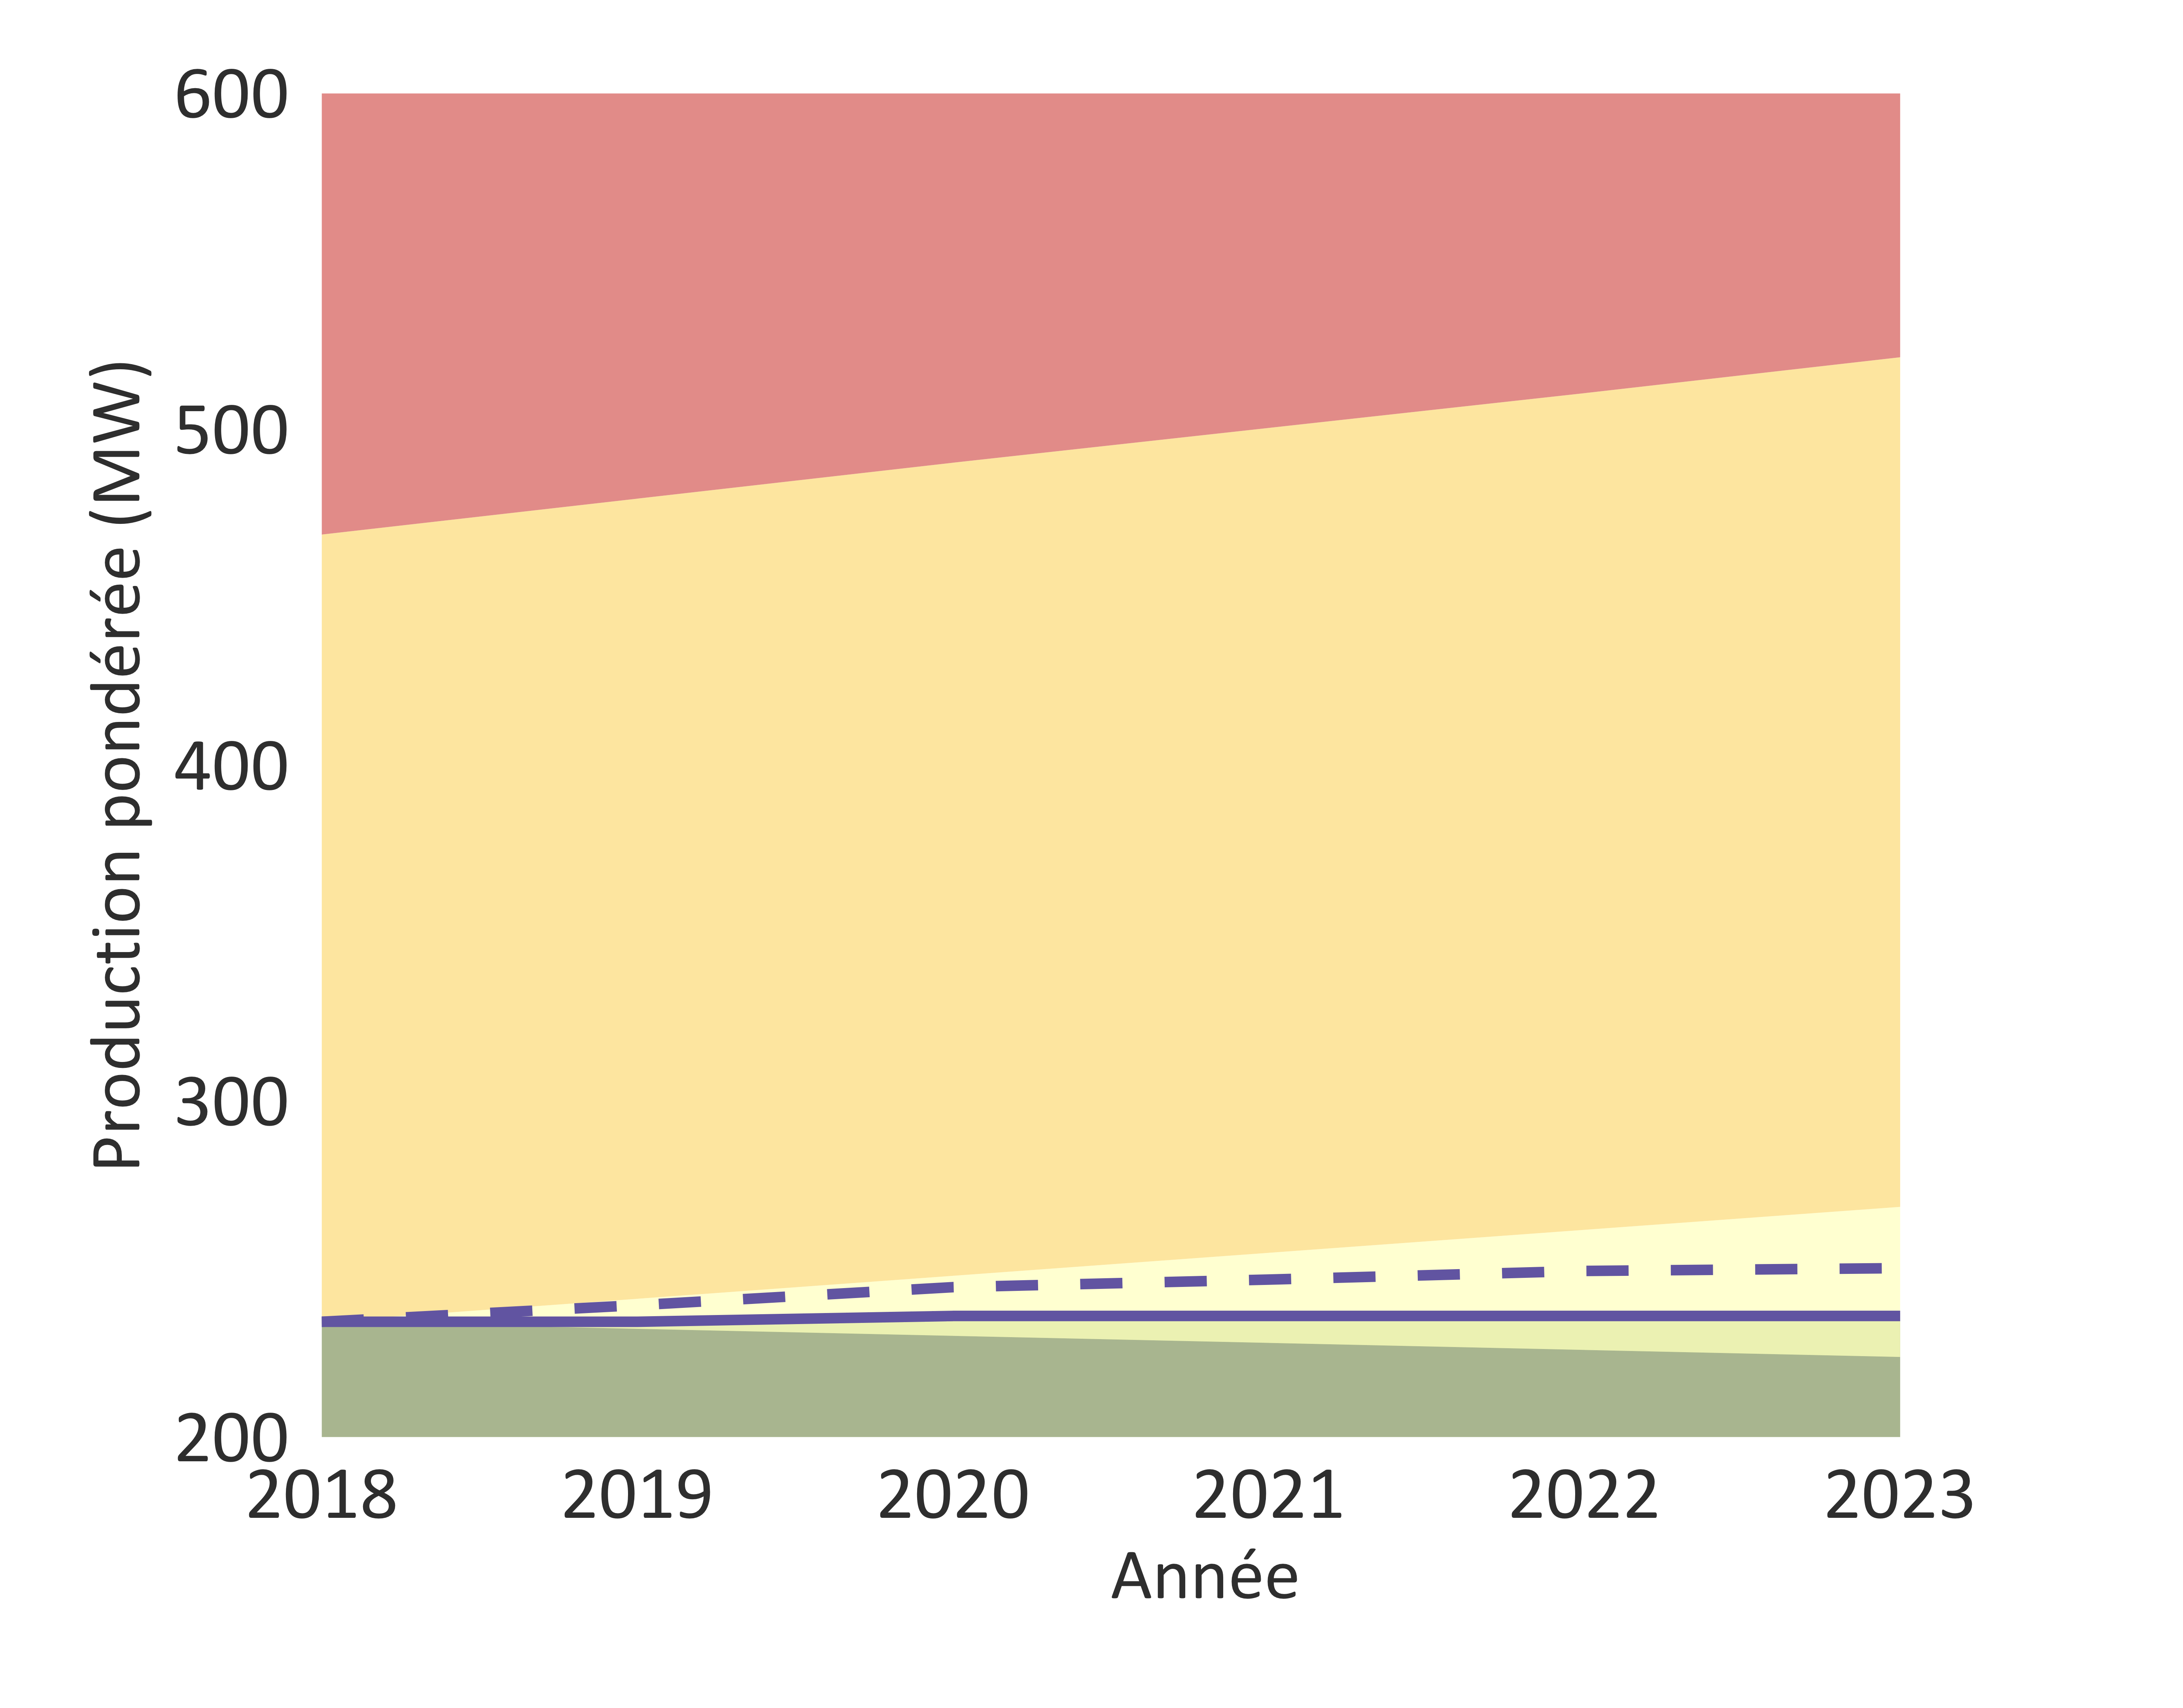
\includegraphics[trim = {0 0cm 0 0},width=1\linewidth]{ReportOutputs/Fig07}
		
		\textbf{Trajectory of Renewable Power Capacity* }
		
		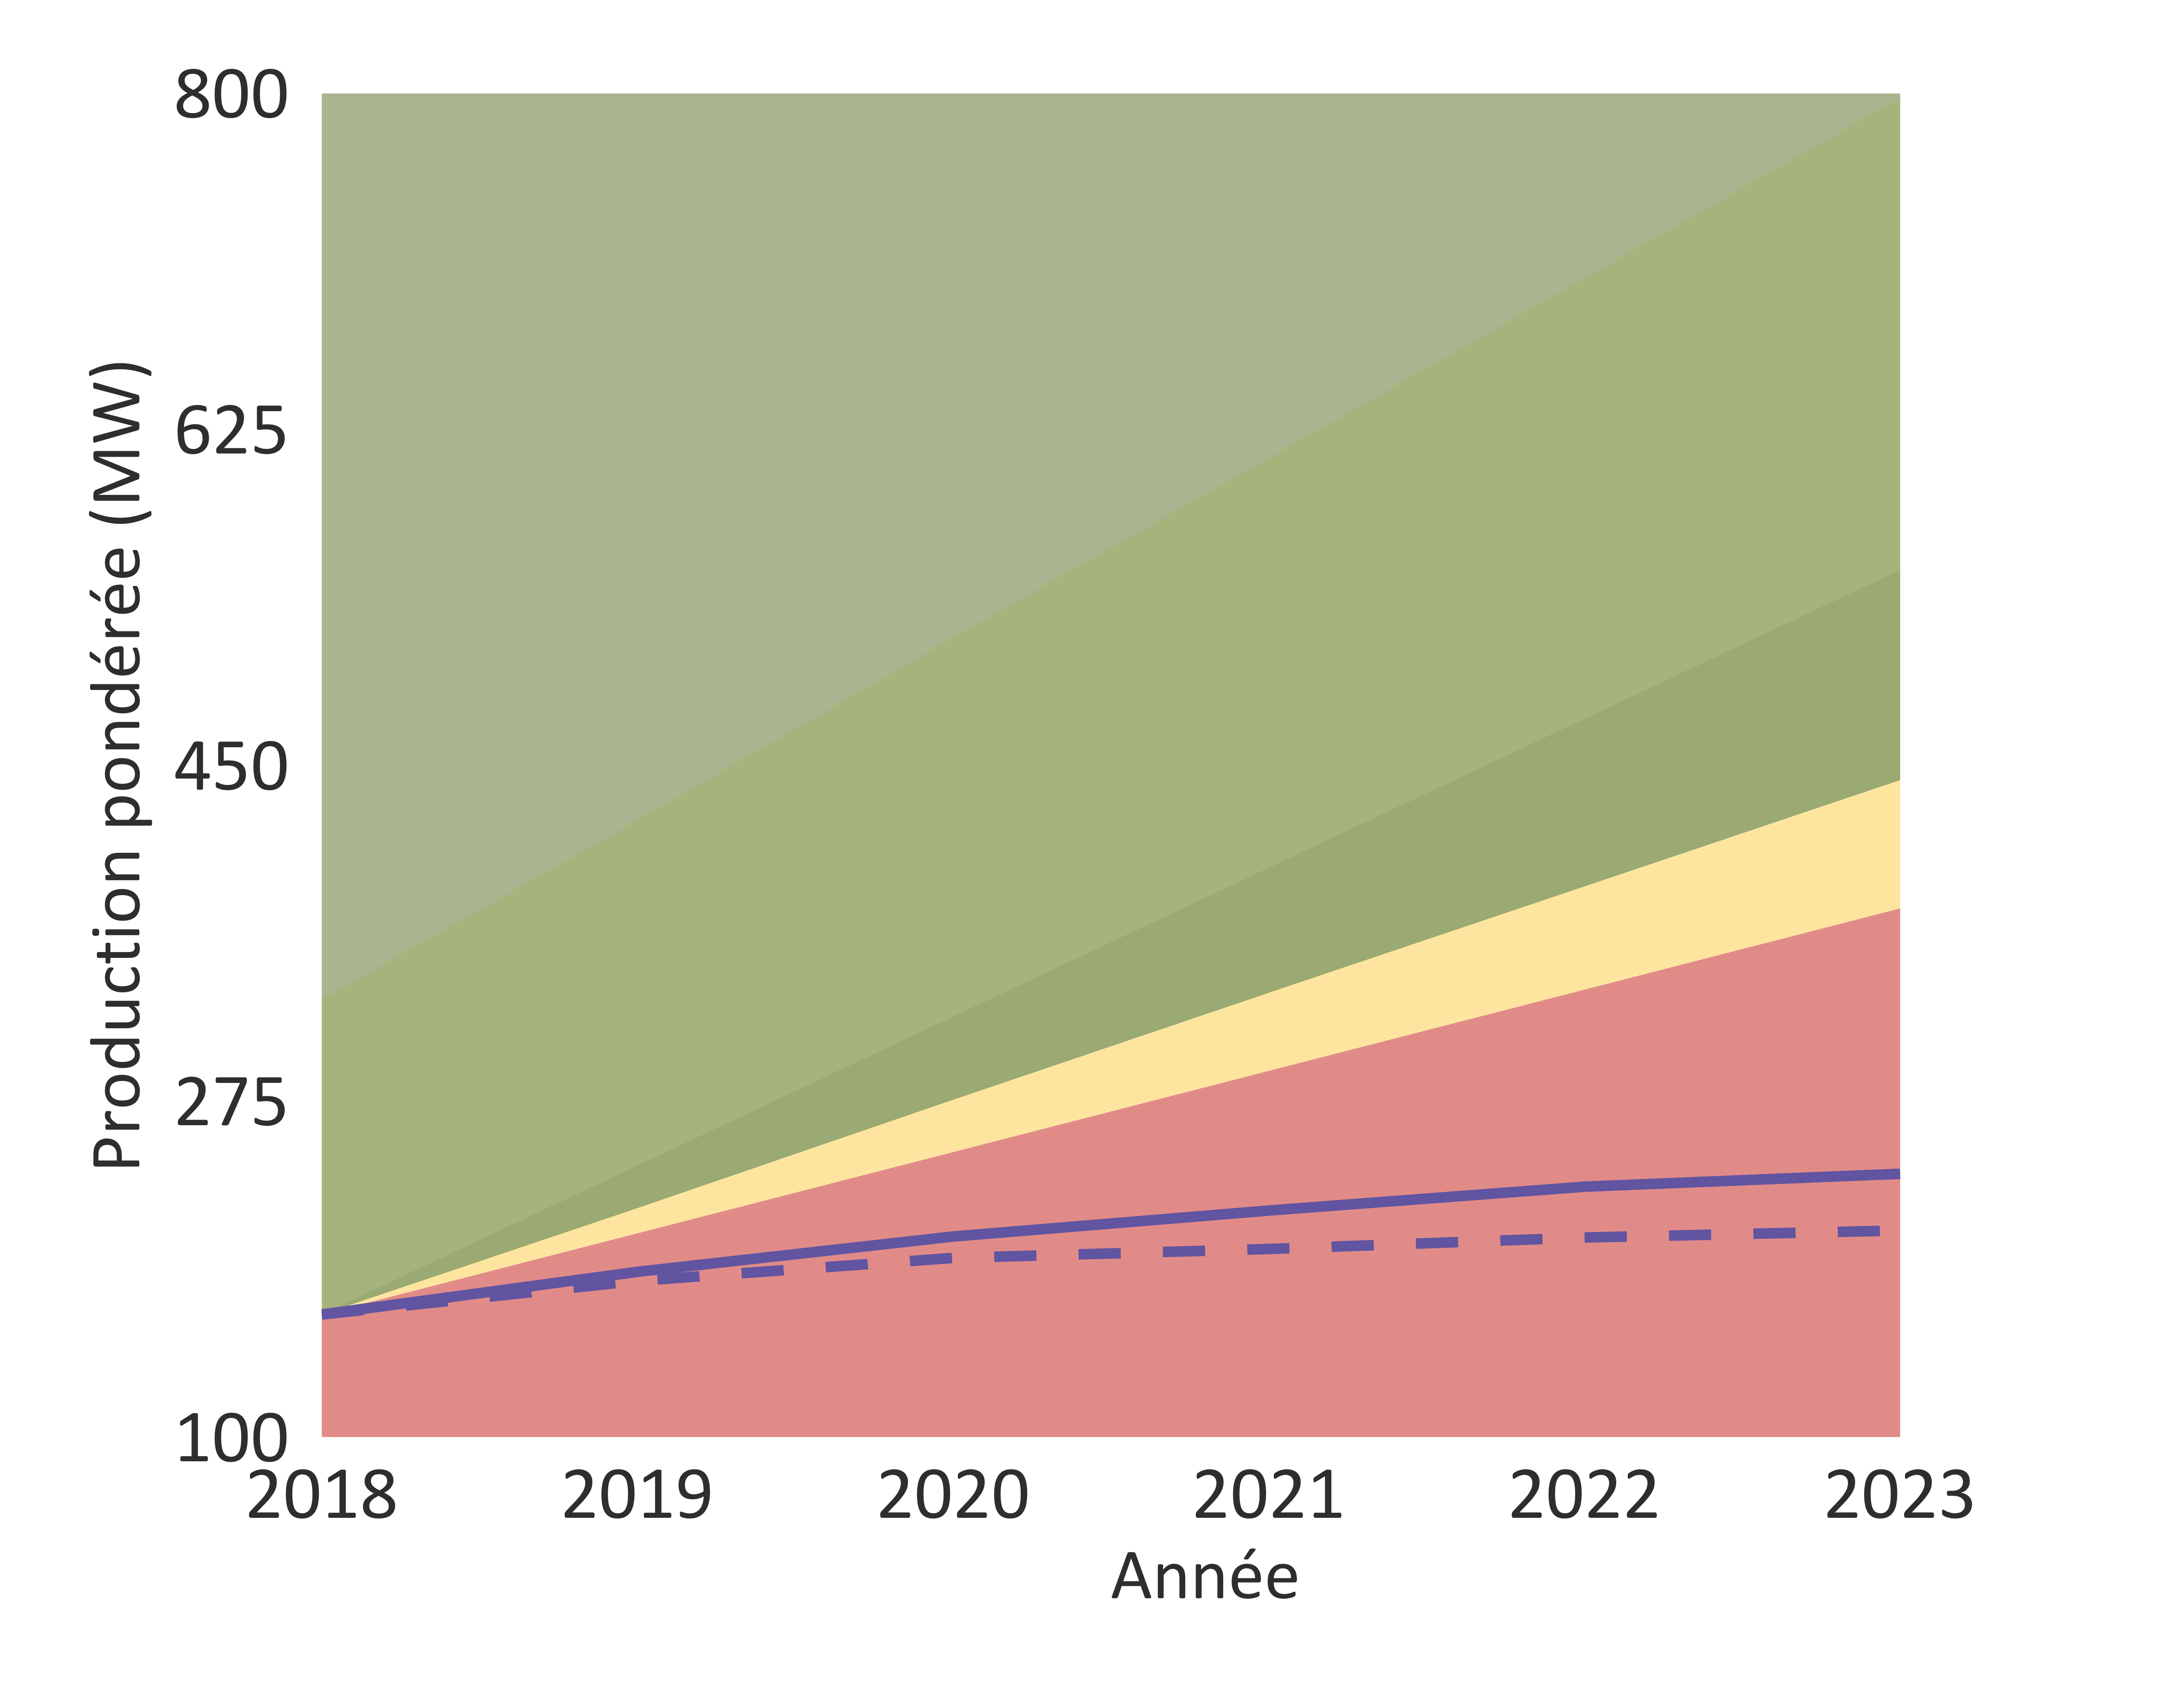
\includegraphics[trim = {0 0cm 0 0},width=.99\linewidth]{ReportOutputs/Fig08}
	\end{minipage}	
	\hspace{.02\linewidth}
	\begin{minipage}[t]{.49\textwidth}
		\textbf{Trajectory of Gas Power Capacity }
		
		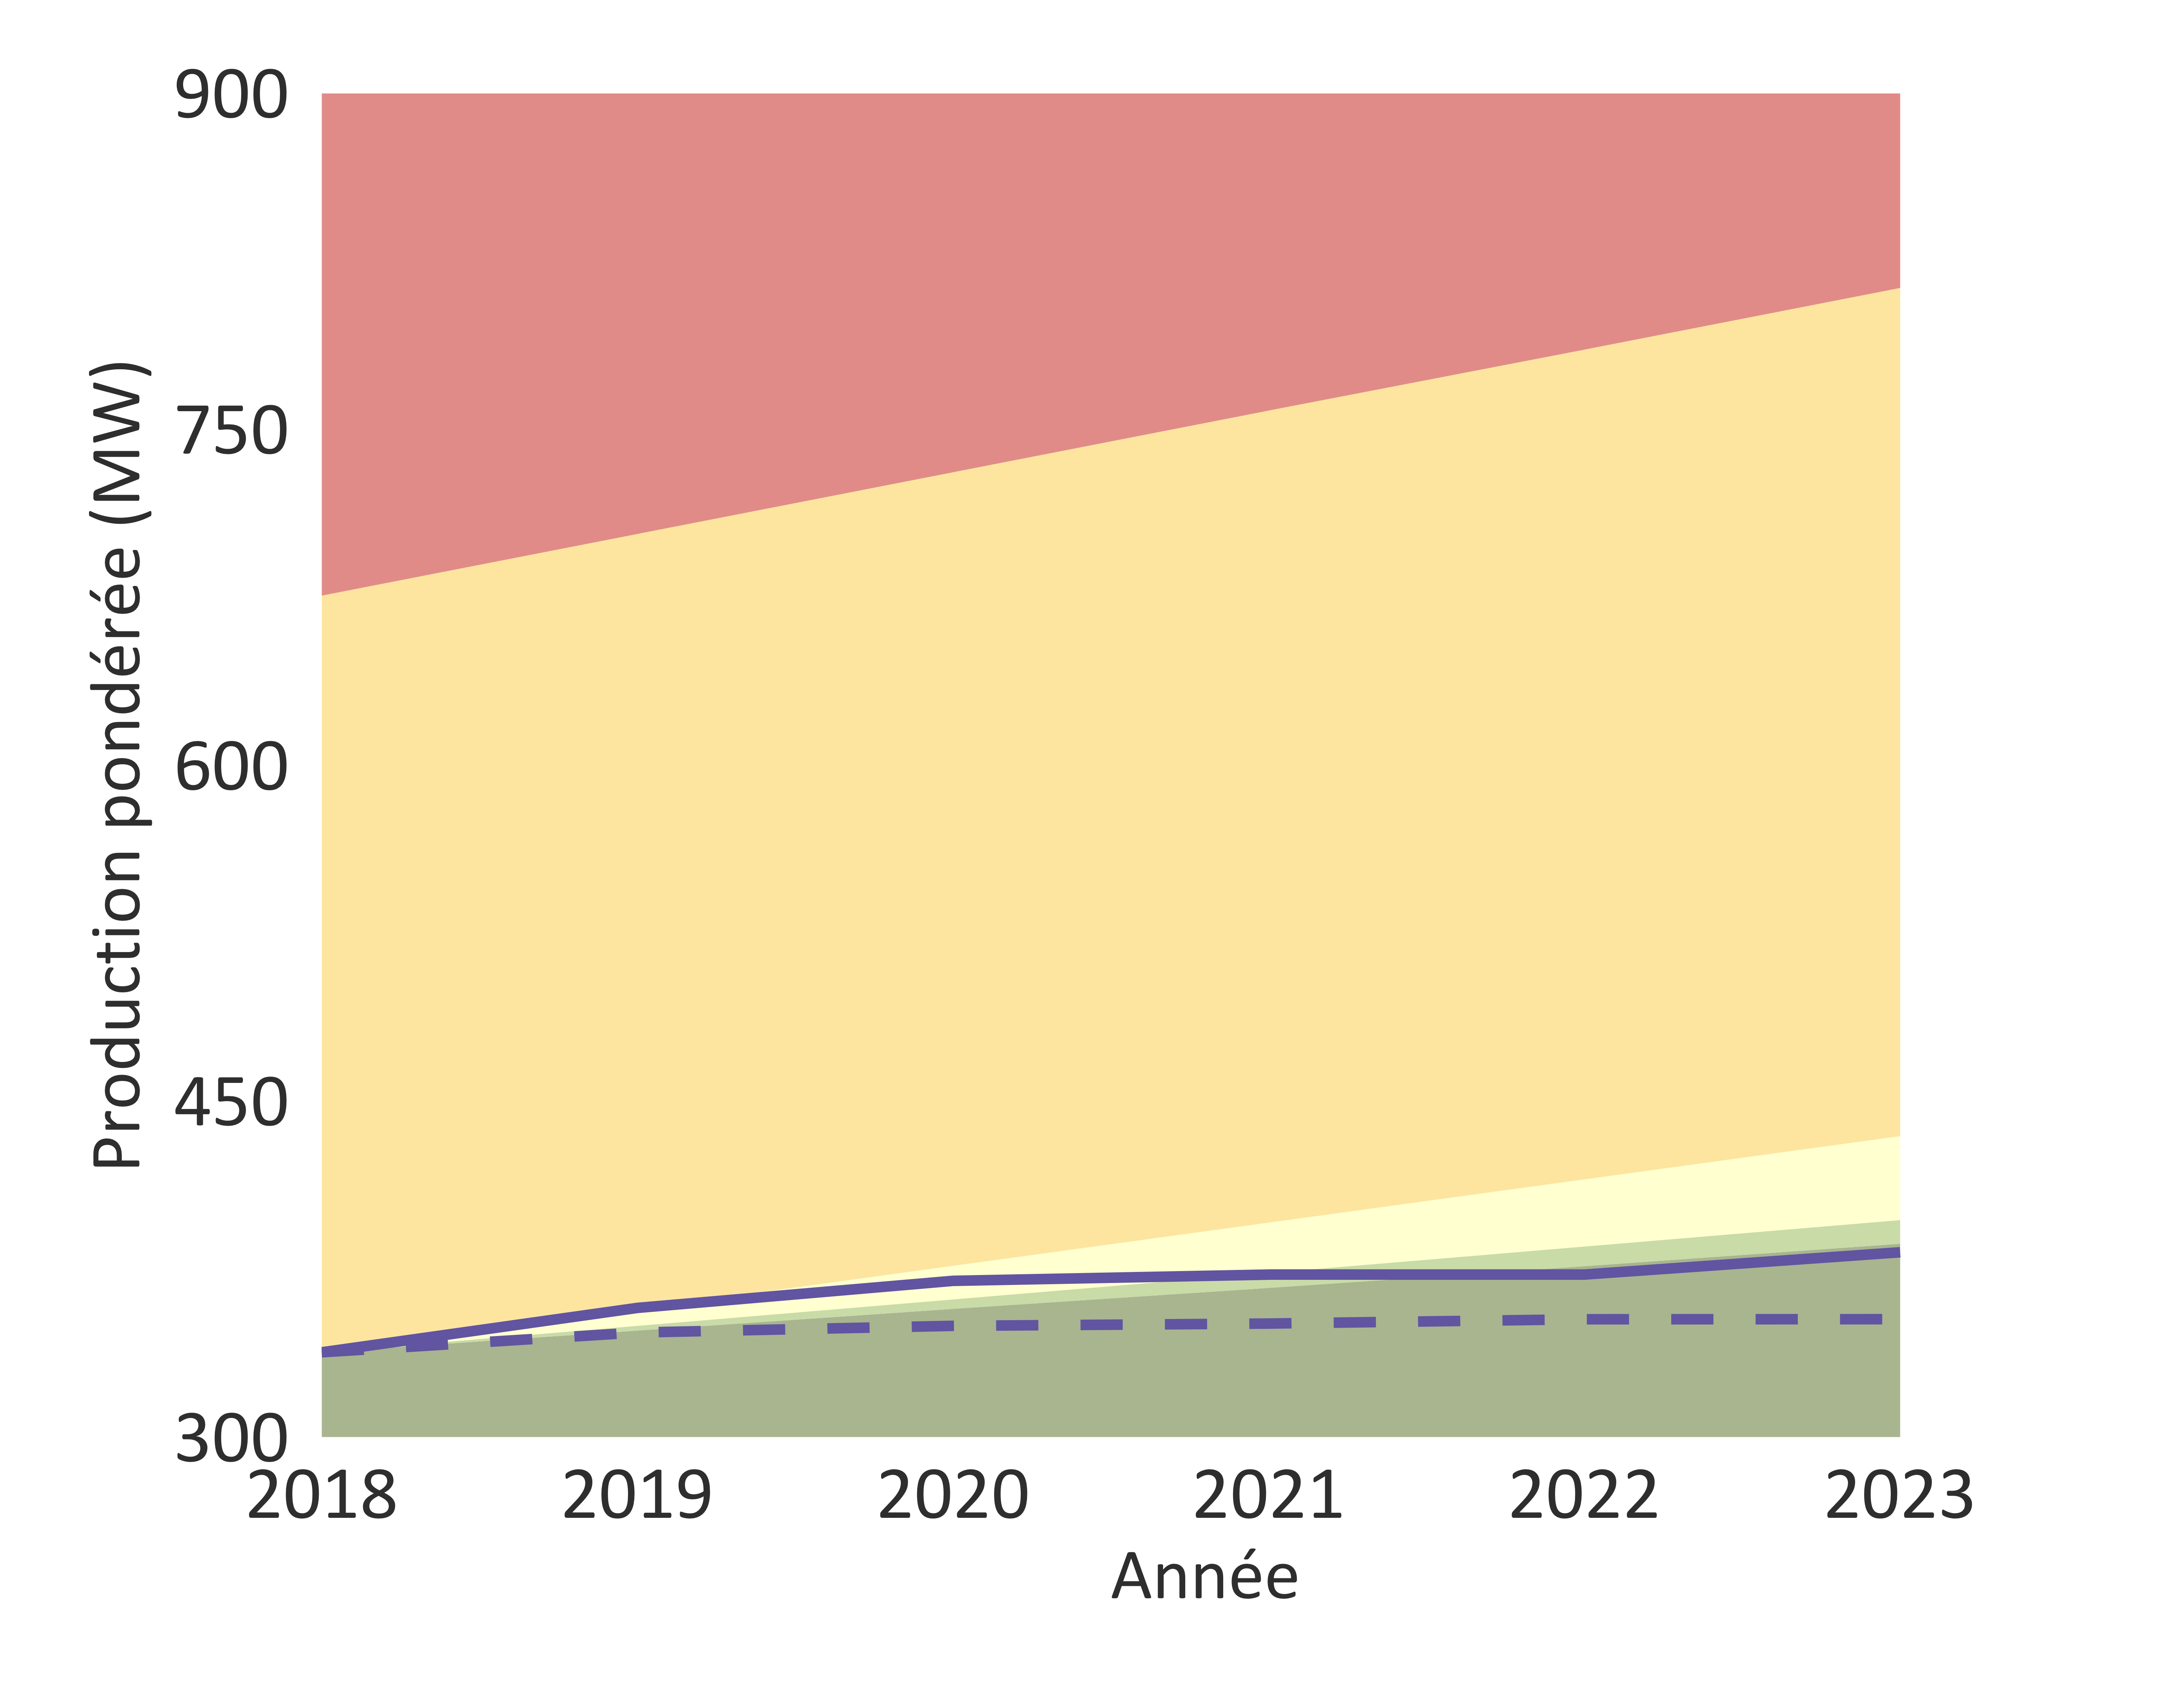
\includegraphics[trim = {0 0cm 0 0},width=1\linewidth]{ReportOutputs/Fig09}
		
		%WWFSpecificExcludeS
		\textbf{Trajectory of Hydro Power Capacity }
		
		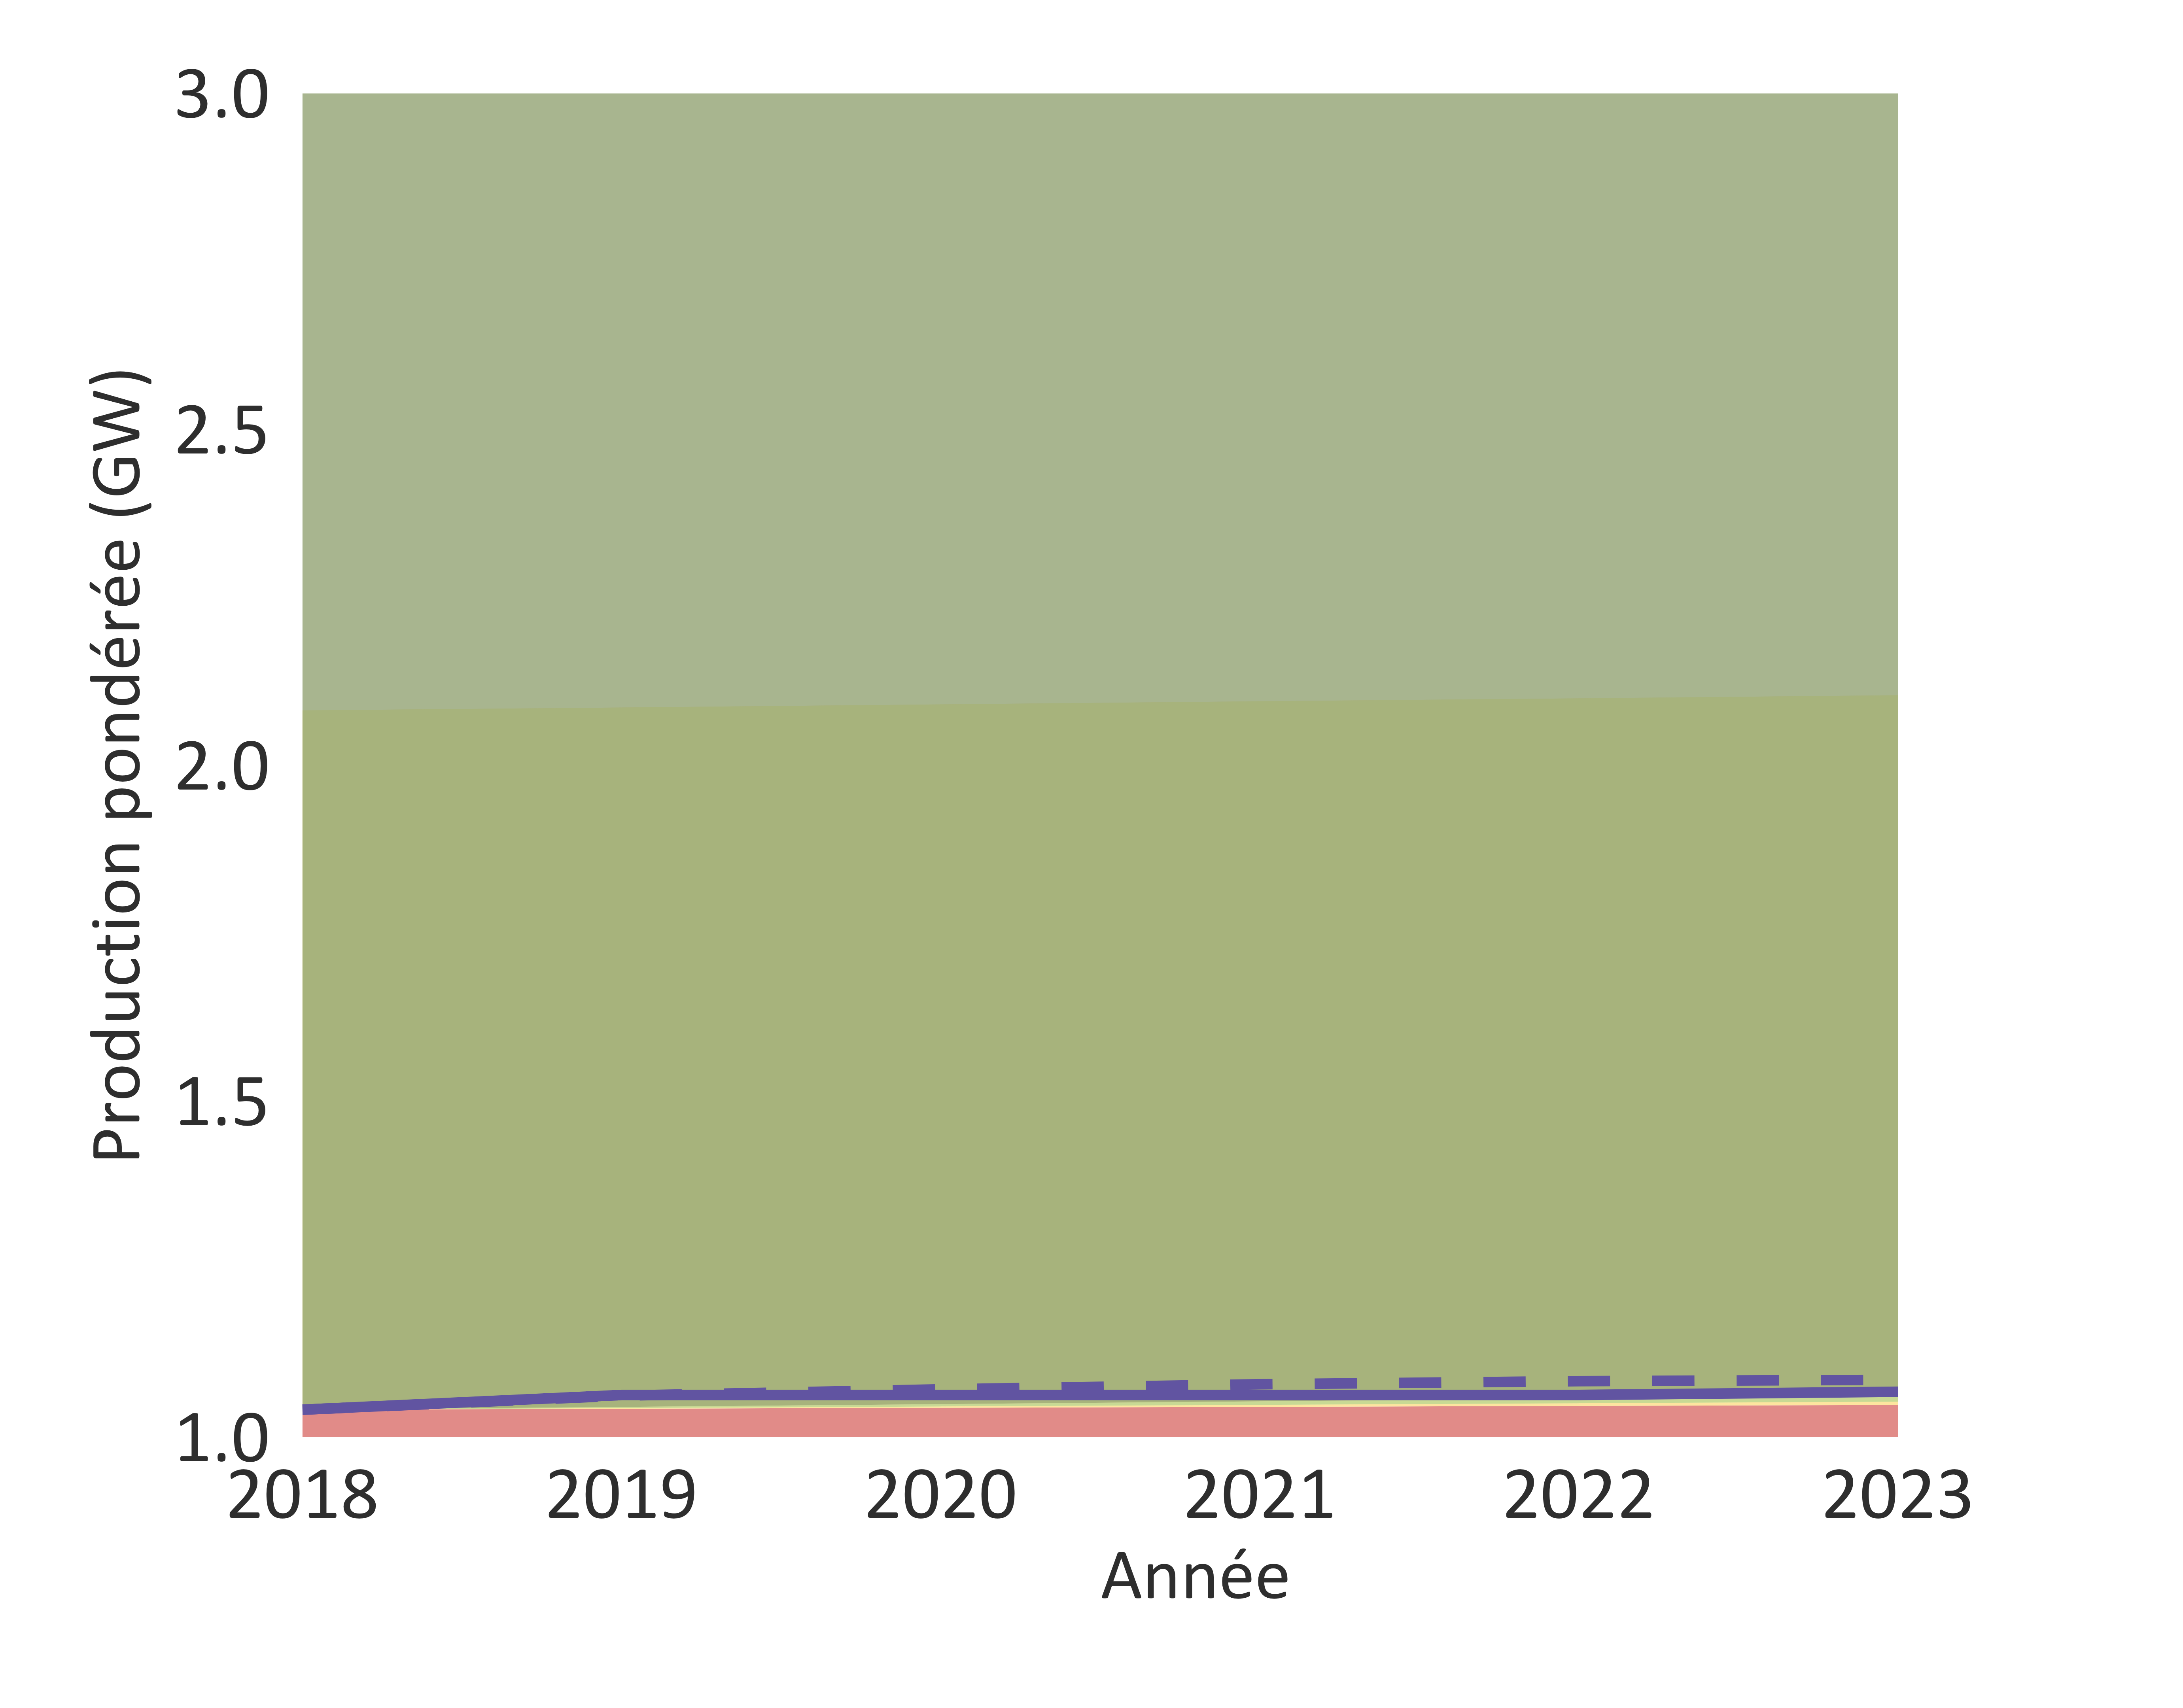
\includegraphics[trim = {0 0cm 0 0},width=1\linewidth]{ReportOutputs/Fig10}
		%WWFSpecificExcludeE
		
	\end{minipage}
	
	\vspace{-0.8cm}
	\begin{center}
		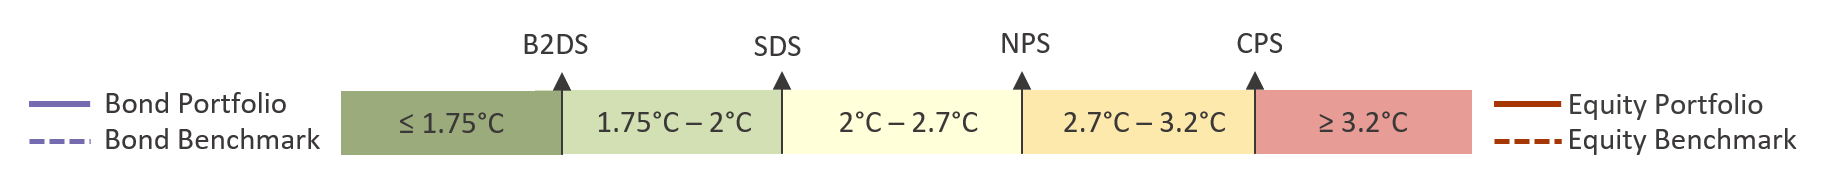
\includegraphics[trim = {0 0cm 0 0},width=.9\linewidth]{ReportGraphics/246Legend.png}
	\end{center}
	
	\small\textit{*Due to differences in assumptions about the technology mix within the renewable power sector between the B2DS and SDS, the SDS may appear more ambitious for renewable energy than the B2DS. However power generation from renewables is still expected to be greater in the B2DS despite the reduced capacity.}
	
	%\PageFooterThird
\PageFooter{3 - TRAJECTORY OF THE PORTFOLIO}
	\newpage 
	%PowerSector_CBE
	%PowerSector_EQS
	\section*{} % TRAJECTORY - EQUITY - POWER  
	\HeaderDouble{5 YEAR TREND - EQUITY}{POWER}		
	
	\begin{multicols}{2}
		\textbf{The alignment graphs below show the alignment of selected power technologies in the equity portfolio relative to the IEA transition scenarios: B2DS (well below 2°C), SDS (2°C), NPS (4°C), CPS (6°C) and the global listed equity market.} 
		For each technology, the value plotted for the portfolio (solid line) is the planned evolution or `trajectory' of installed capacity allocated to the equity portfolio over the next 5 years. The lines separating the color-coded background areas plot the portfolio's `target production' for each technology under the IEA scenarios. The dotted line shows the planned trajectory of installed capacity in the specific technology for the listed equity market, scaled to the same starting point as the portfolio.                    
		
	\end{multicols}
	
	
	
	\begin{minipage}[t]{.49\linewidth}
		\textbf{Trajectory of Coal Power Capacity }
		
		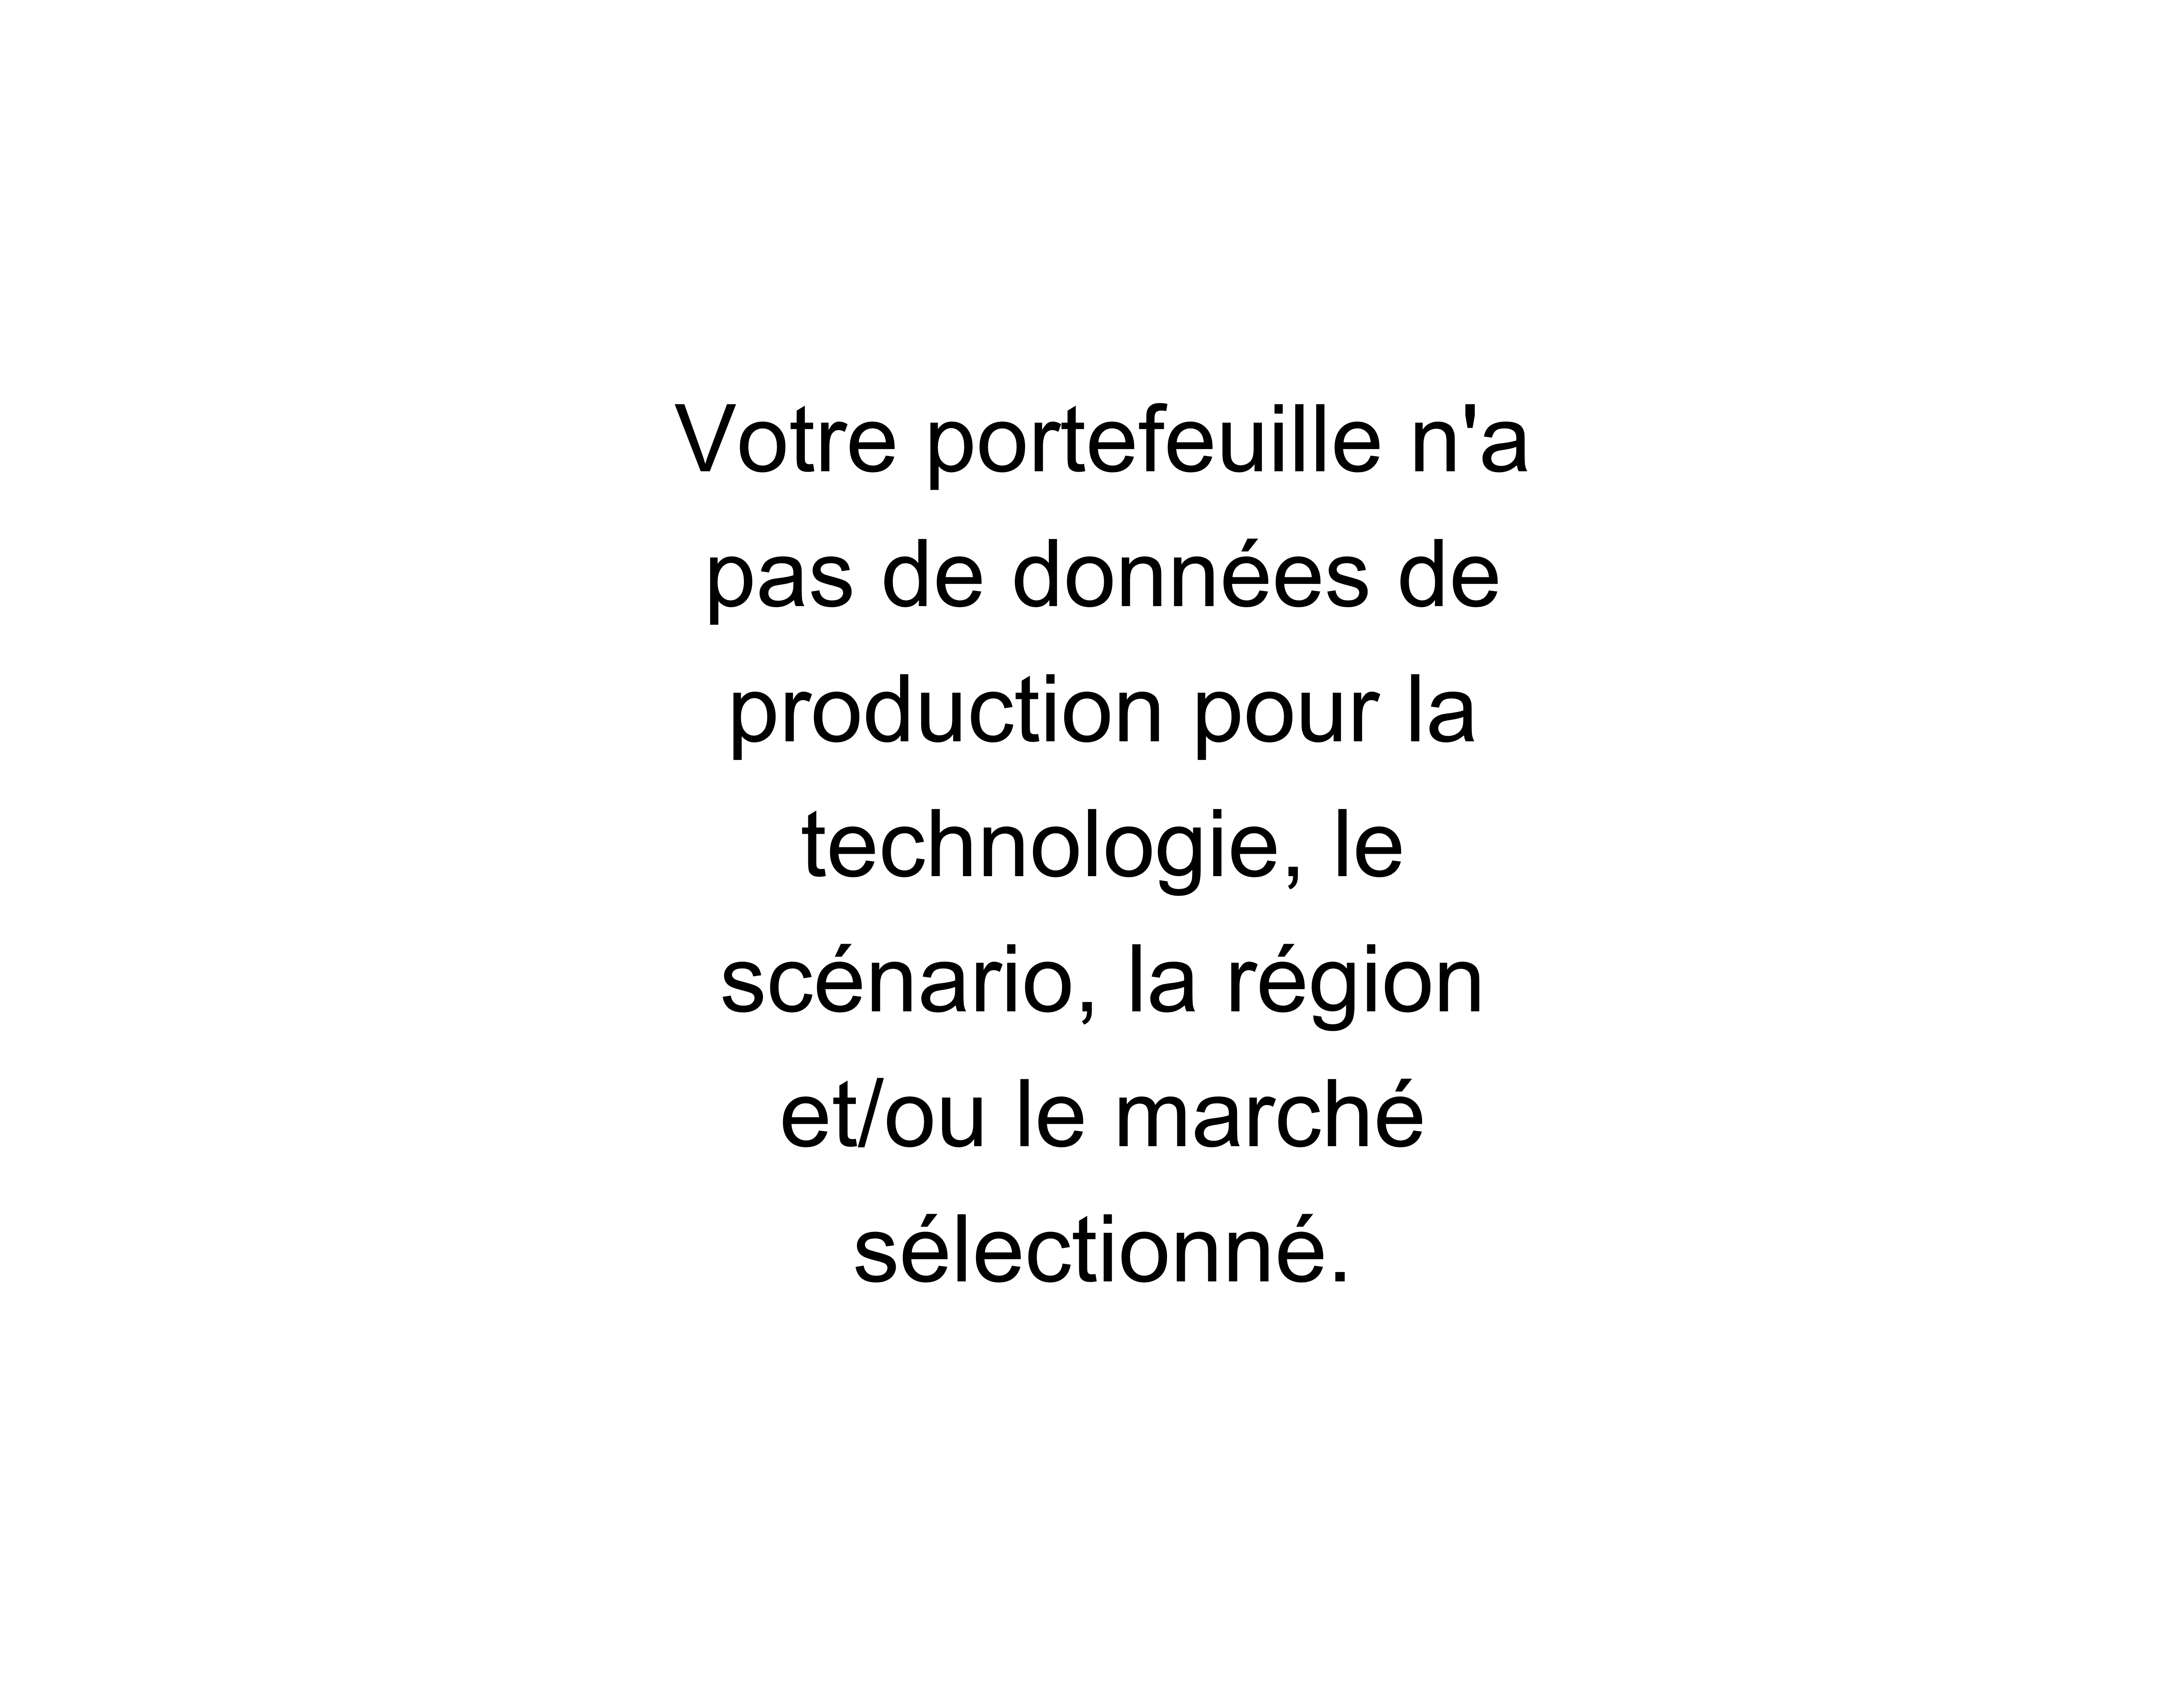
\includegraphics[trim = {0 0cm 0 0},width=1\linewidth]{ReportOutputs/Fig17}
		
		\textbf{Trajectory of Renewable Power Capacity* }
		
		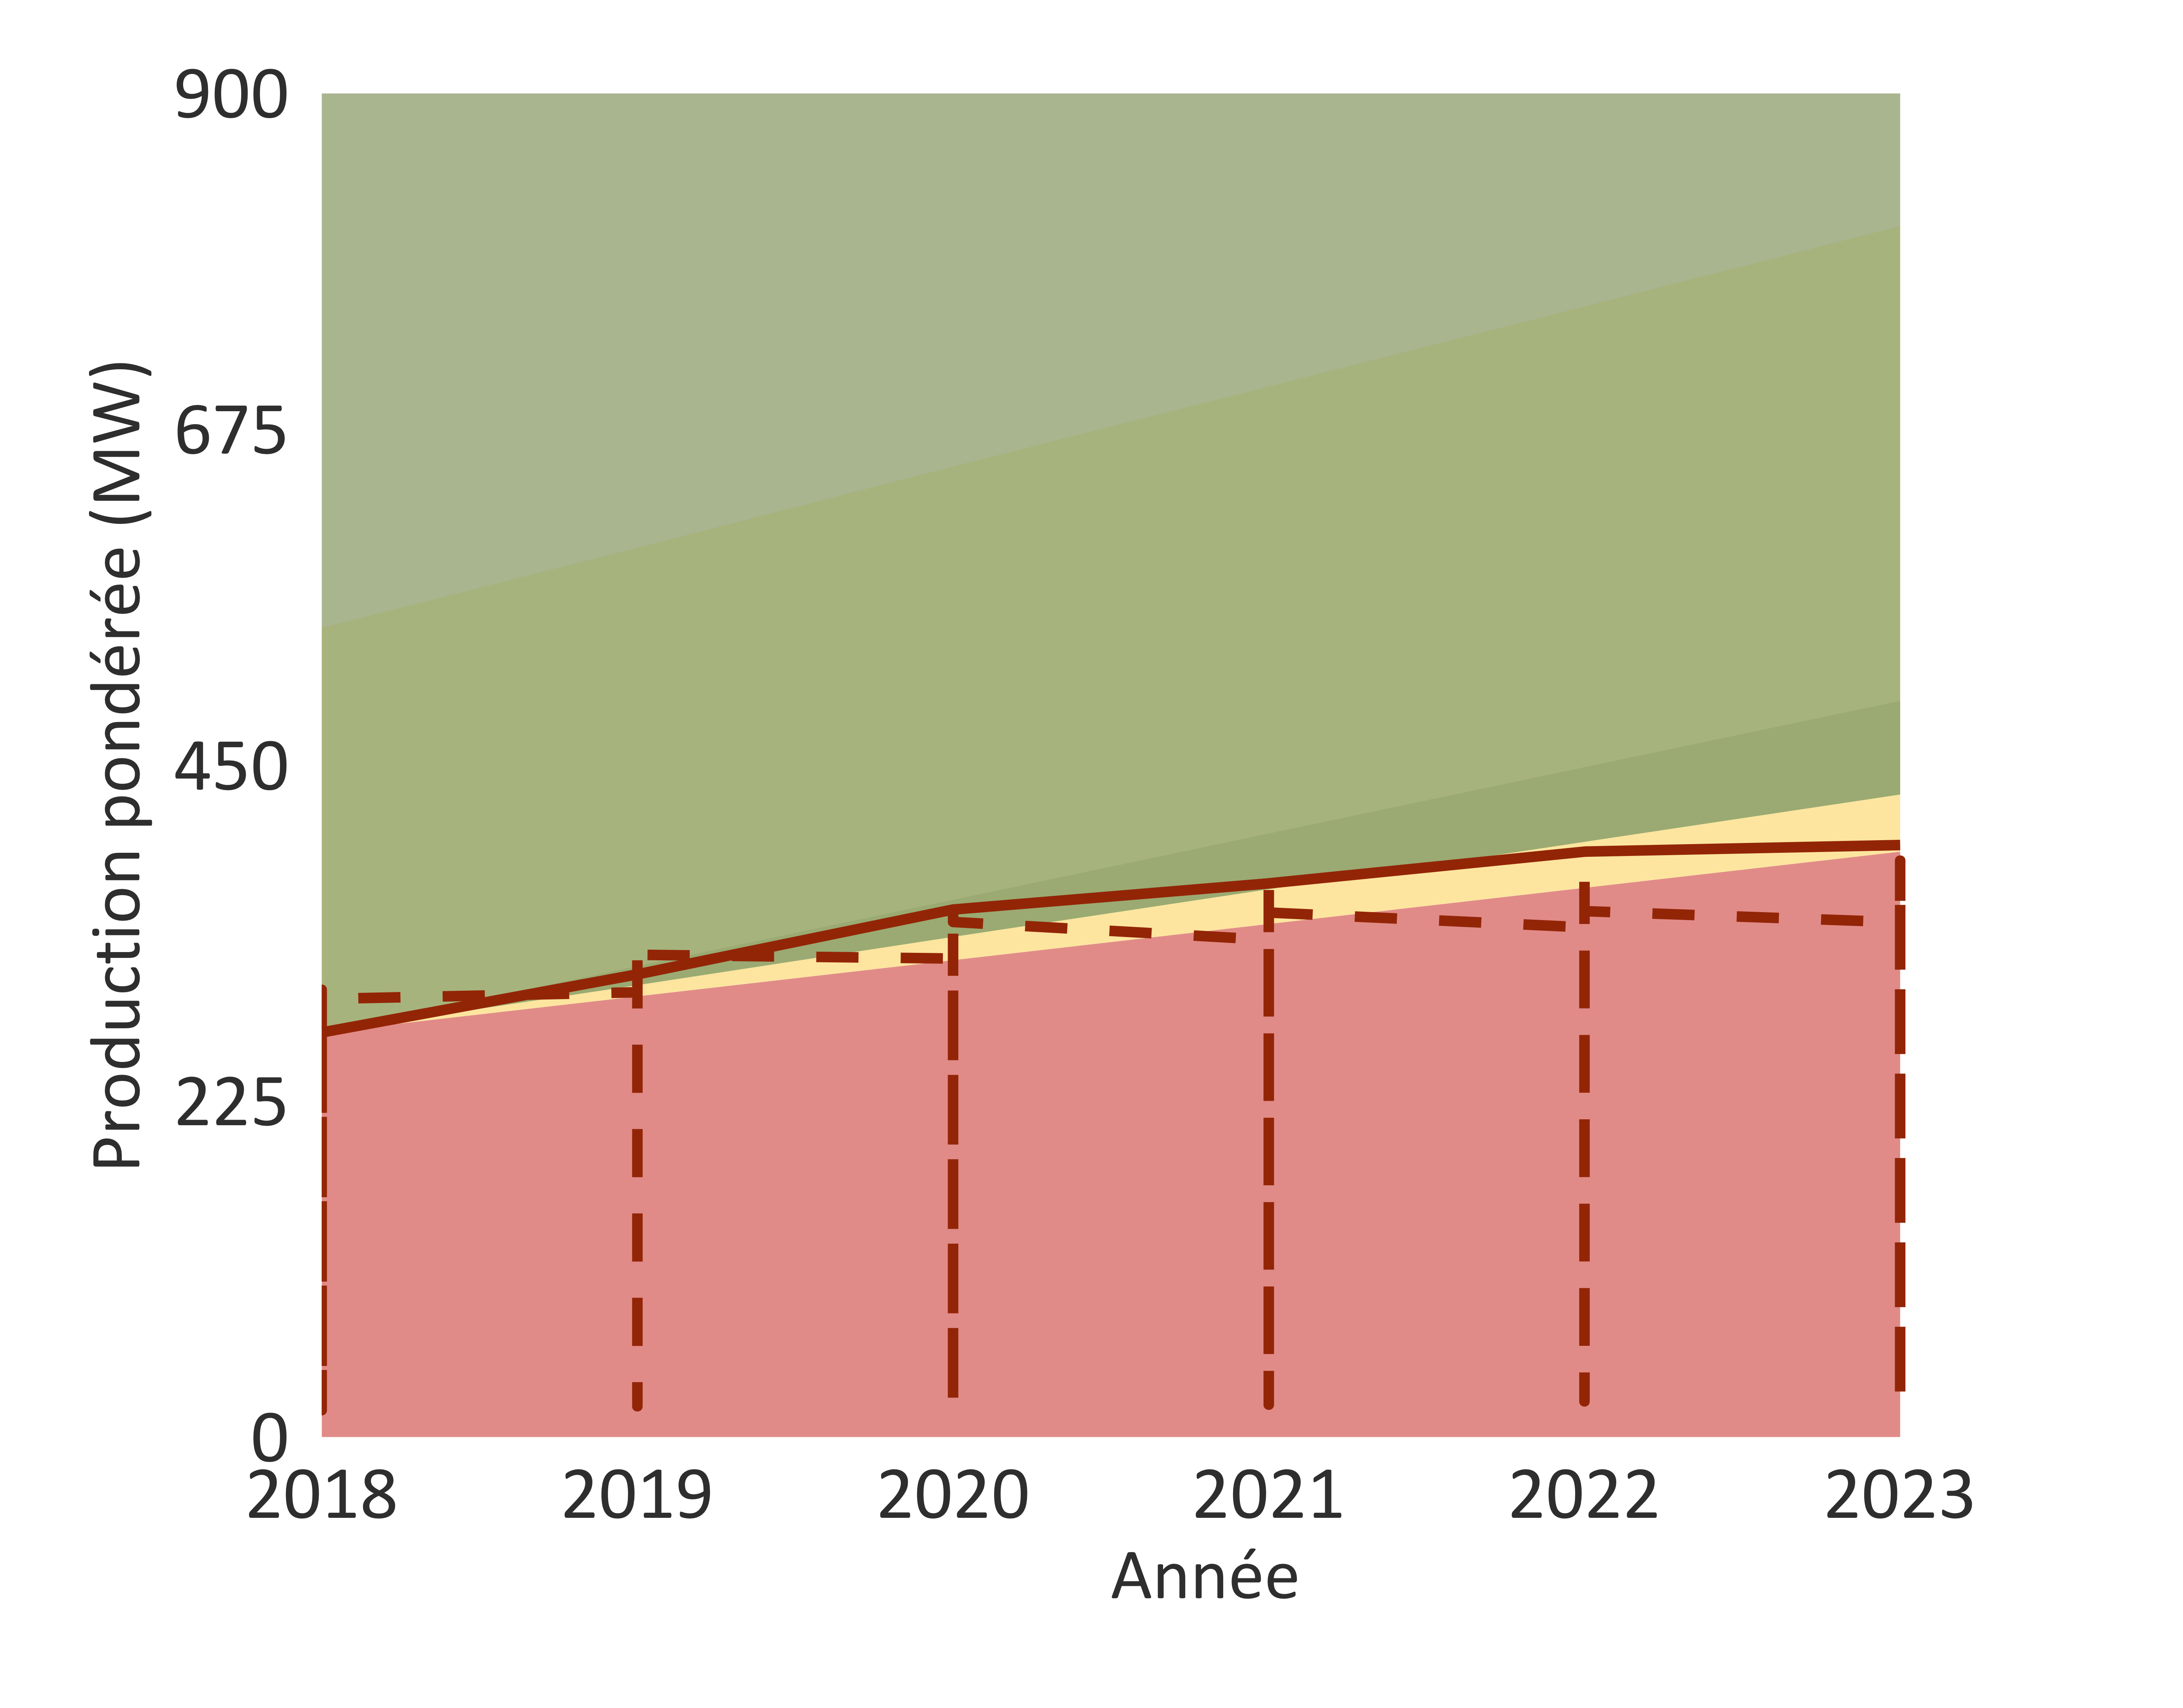
\includegraphics[trim = {0 0cm 0 0},width=.99\linewidth]{ReportOutputs/Fig18}
	\end{minipage}	
	\hspace{.02\linewidth}
	\begin{minipage}[t]{.49\textwidth}
		\textbf{Trajectory of Gas Power Capacity }
		
		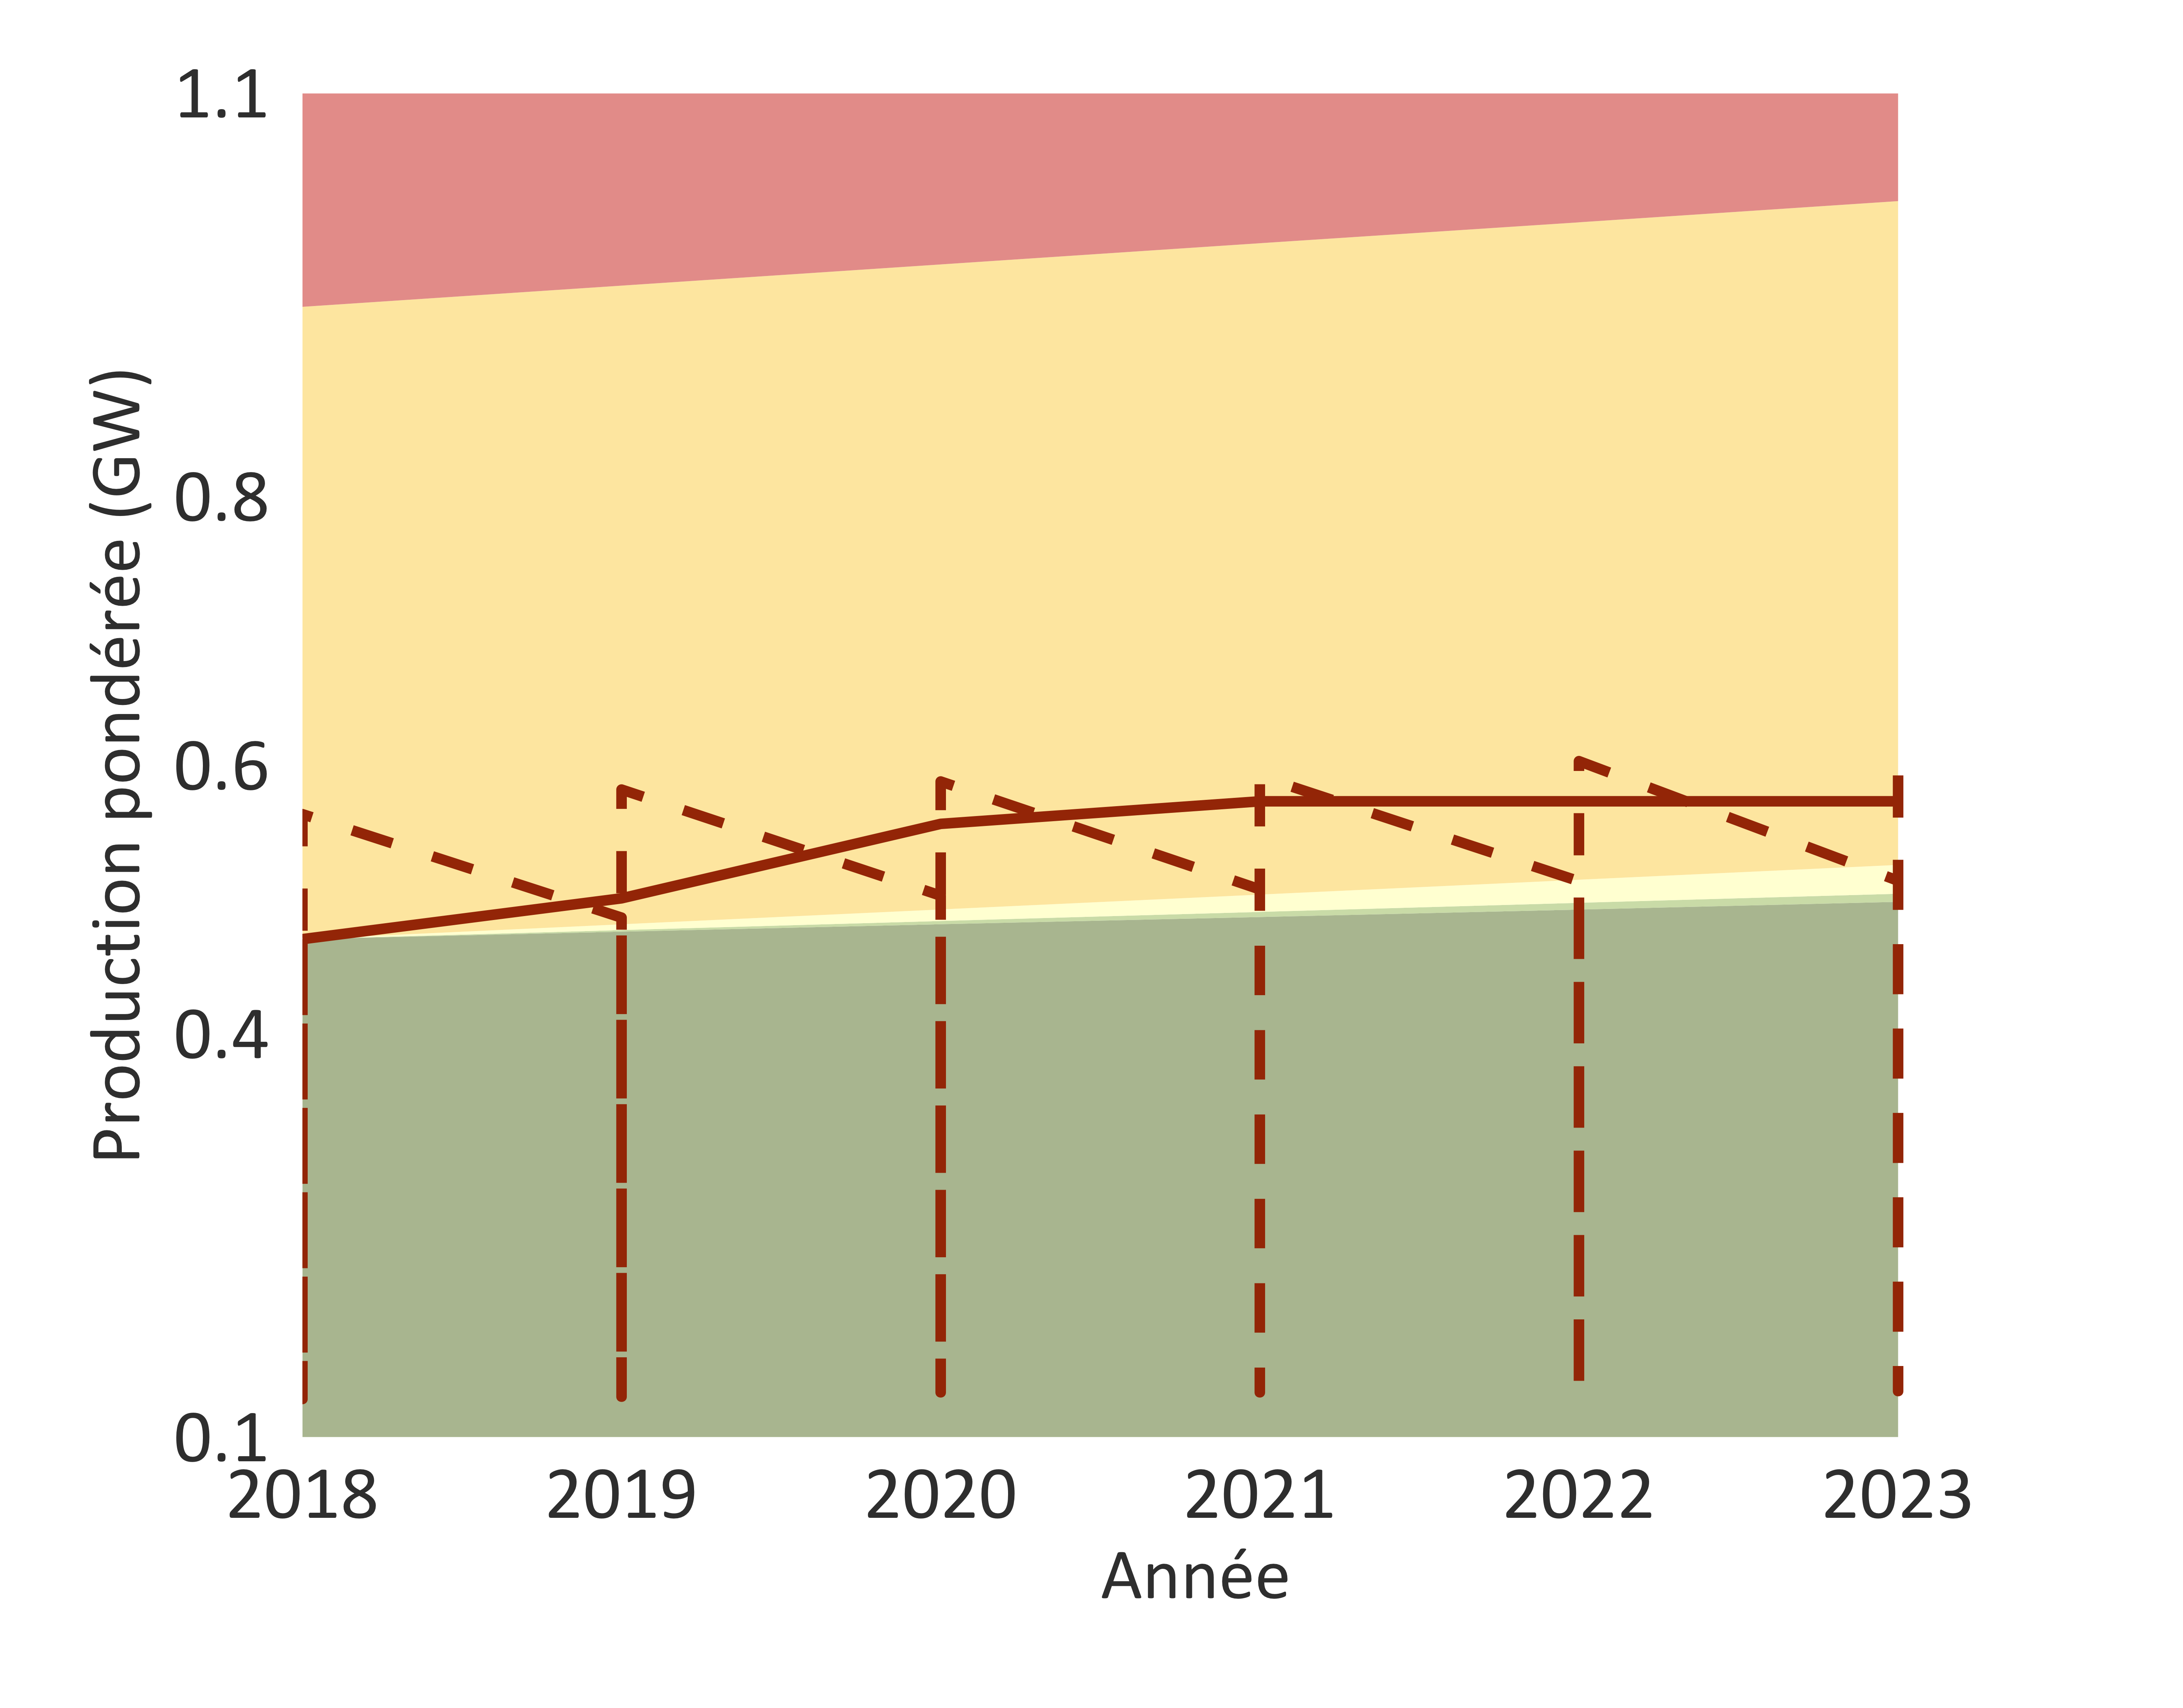
\includegraphics[trim = {0 0cm 0 0},width=1\linewidth]{ReportOutputs/Fig19}
		
		%WWFSpecificExcludeS
		\textbf{Trajectory of Hydro Power Capacity }
		
		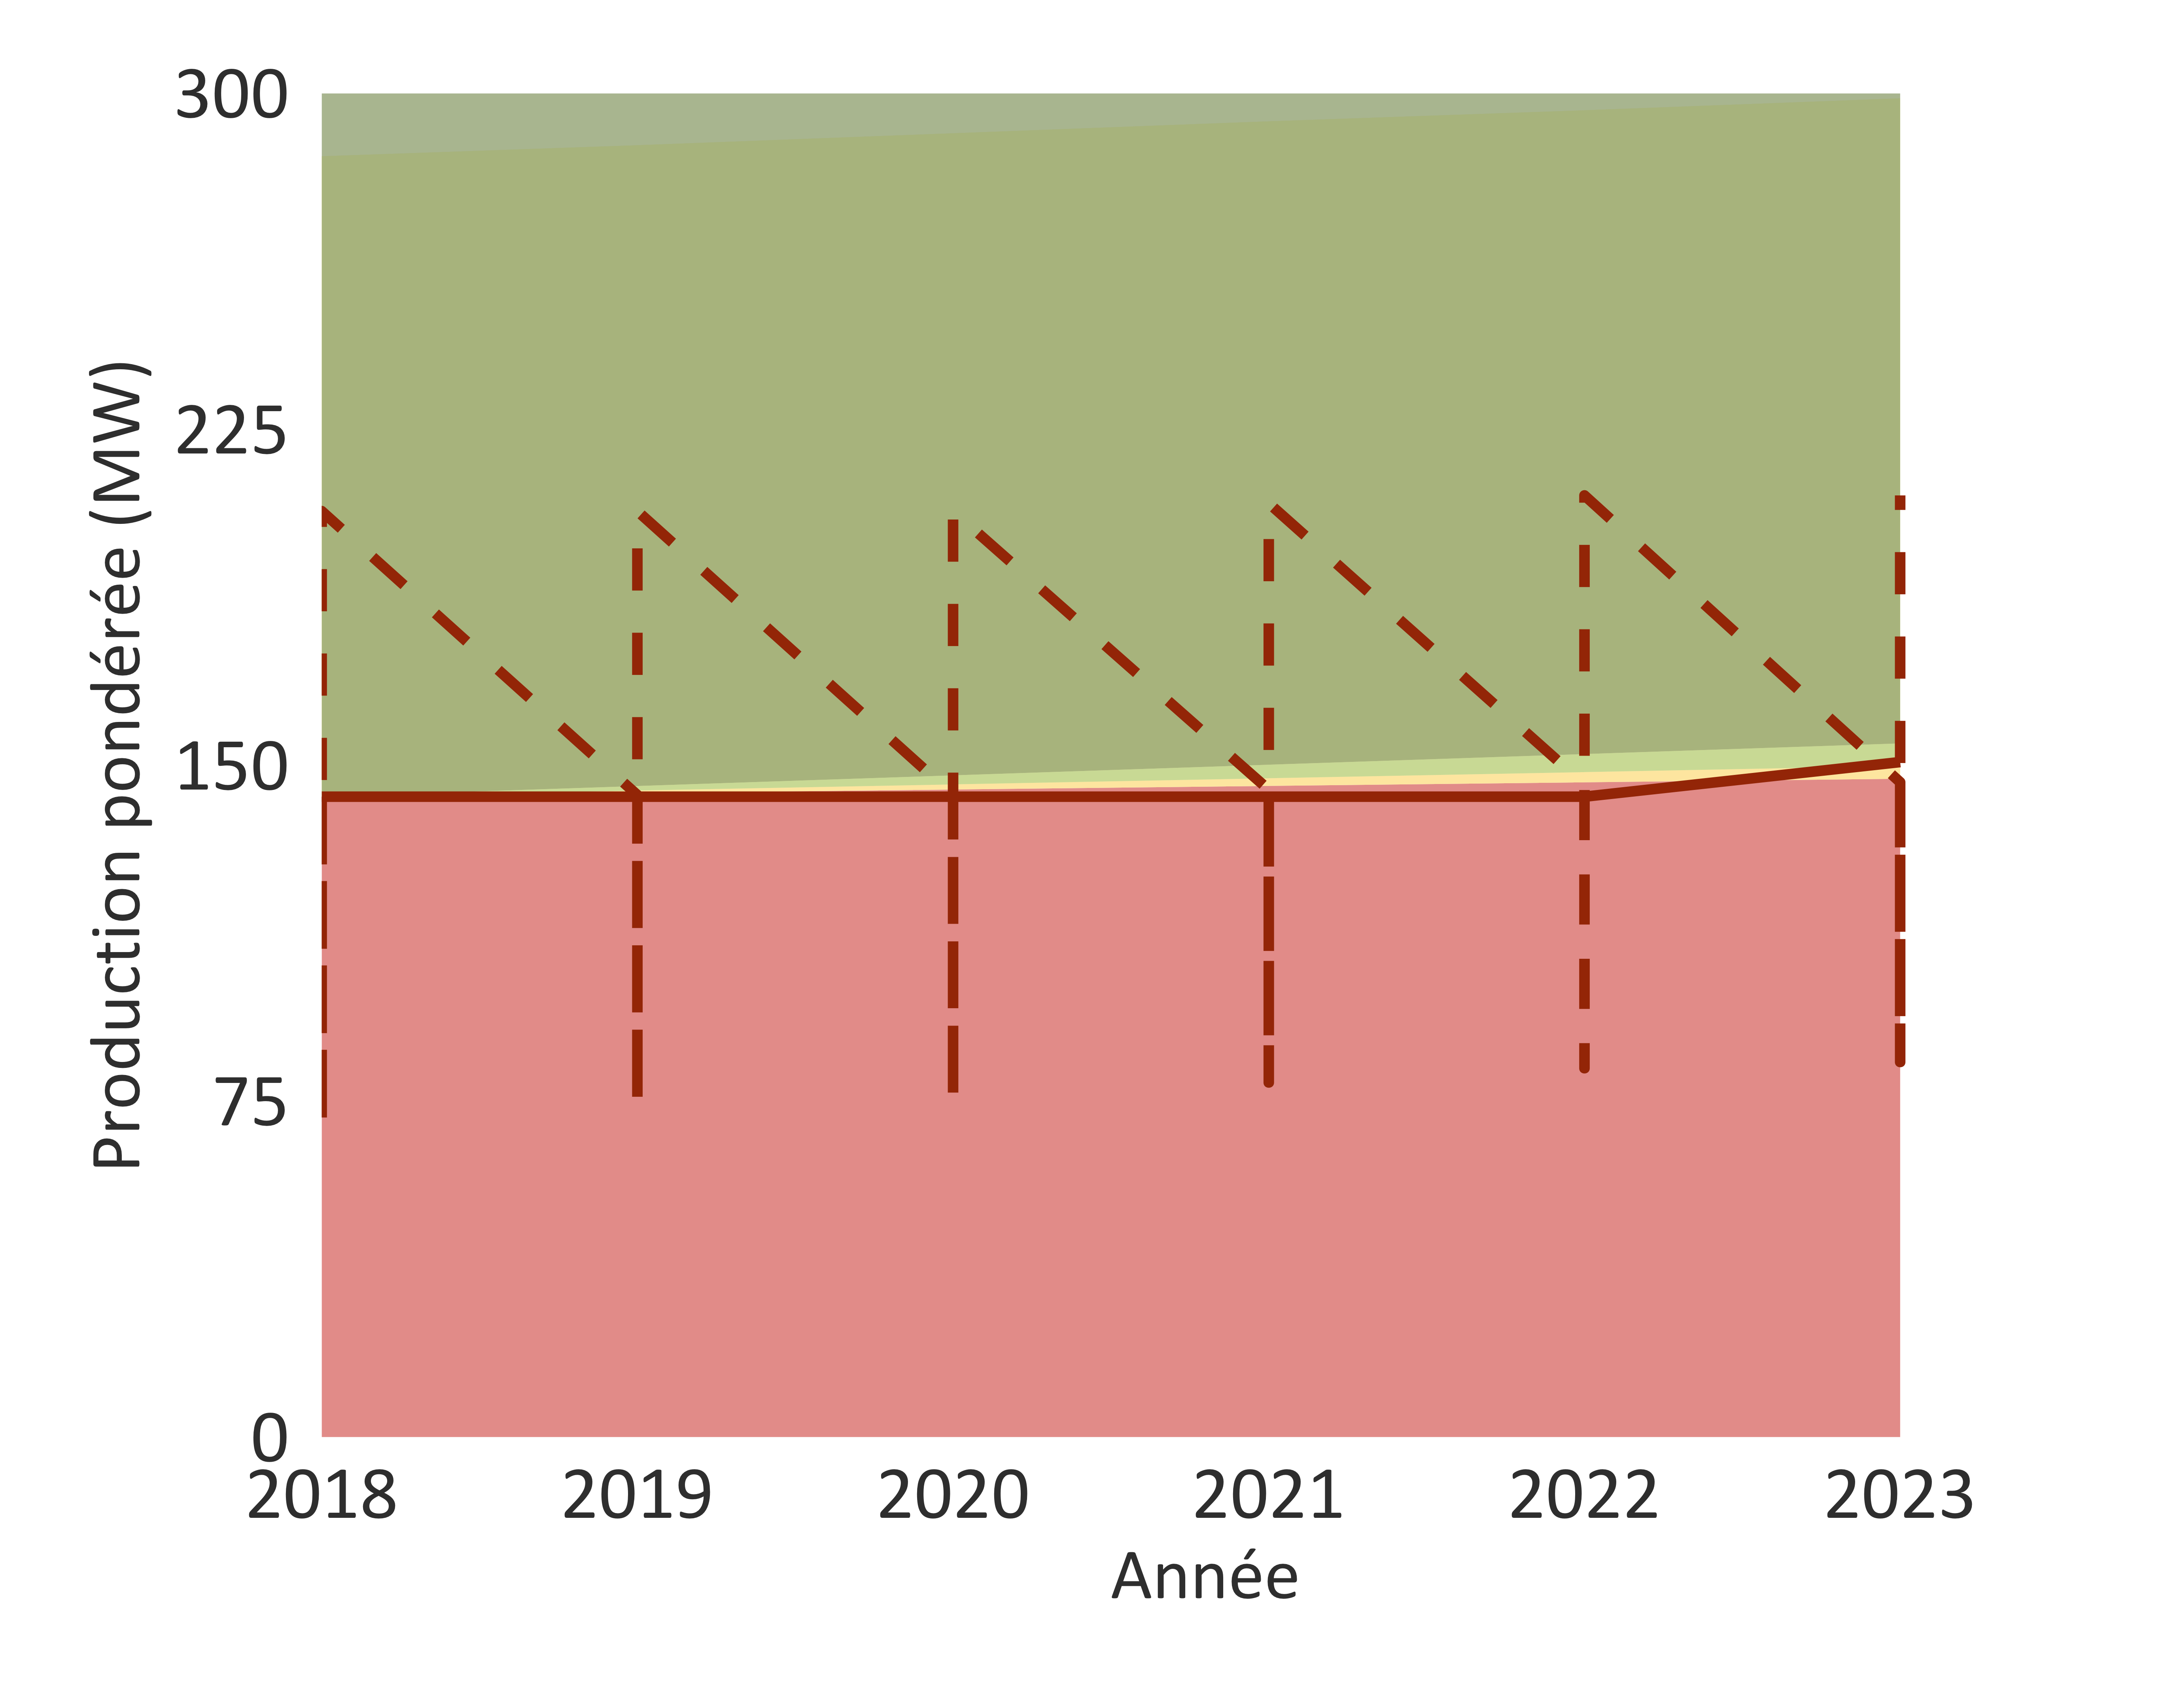
\includegraphics[trim = {0 0cm 0 0},width=1\linewidth]{ReportOutputs/Fig20}
		%WWFSpecificExcludeE
		
	\end{minipage}
	
	\vspace{-0.6cm}
	\begin{center}
		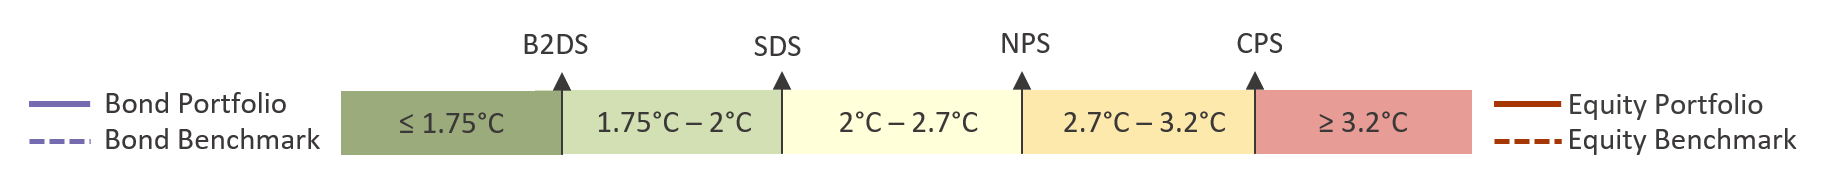
\includegraphics[trim = {0 0cm 0 0},width=.9\linewidth]{ReportGraphics/246Legend.png}
	\end{center}

	\small\textit{*Due to differences in assumptions about the technology mix within the renewable power sector between the B2DS and SDS, the SDS may appear more ambitious for renewable energy than the B2DS. However power generation from renewables is still expected to be greater in the B2DS despite the reduced capacity.}
	
	
	%\PageFooterThird
\PageFooter{3 - TRAJECTORY OF THE PORTFOLIO}
	\newpage 
	%PowerSector_EQE
	%PowerSector_ALLE

	%FossilFuelSector_ALLS
	%FossilFuelSector_CBS
	\section*{} % TRAJECTORY - DEBT - FOSSIL FUELS AND AUTOMOTIVE   
	\HeaderDouble{5 YEAR TREND - CORPORATE BONDS}{FOSSIL FUELS}	
	
	\begin{multicols}{2}
		\textbf{The alignment graphs below show the alignment of fossil fuels in the corporate bond portfolio relative to the IEA transition scenarios: B2DS (well below 2°C), SDS (2°C), NPS (4°C), CPS (6°C) and the bond market. } 
		For each technology, the value plotted for the portfolio (solid line) is the planned evolution or `trajectory' of fossil fuel production allocated to the corporate bond portfolio over the next 5 years. The lines separating the color-coded background areas plot the portfolio's `target production' for each technology under the IEA scenarios. The dotted line shows planned production in the specific technology for the bond market, scaled to the same starting point as the portfolio.                    
		
		
	\end{multicols}		
	
	\begin{center}
		\textbf{Fossil Fuel Sector}
	\end{center}
	
	\begin{minipage}[t]{.49\linewidth}
		\textbf{Trajectory of Oil Production }
		
		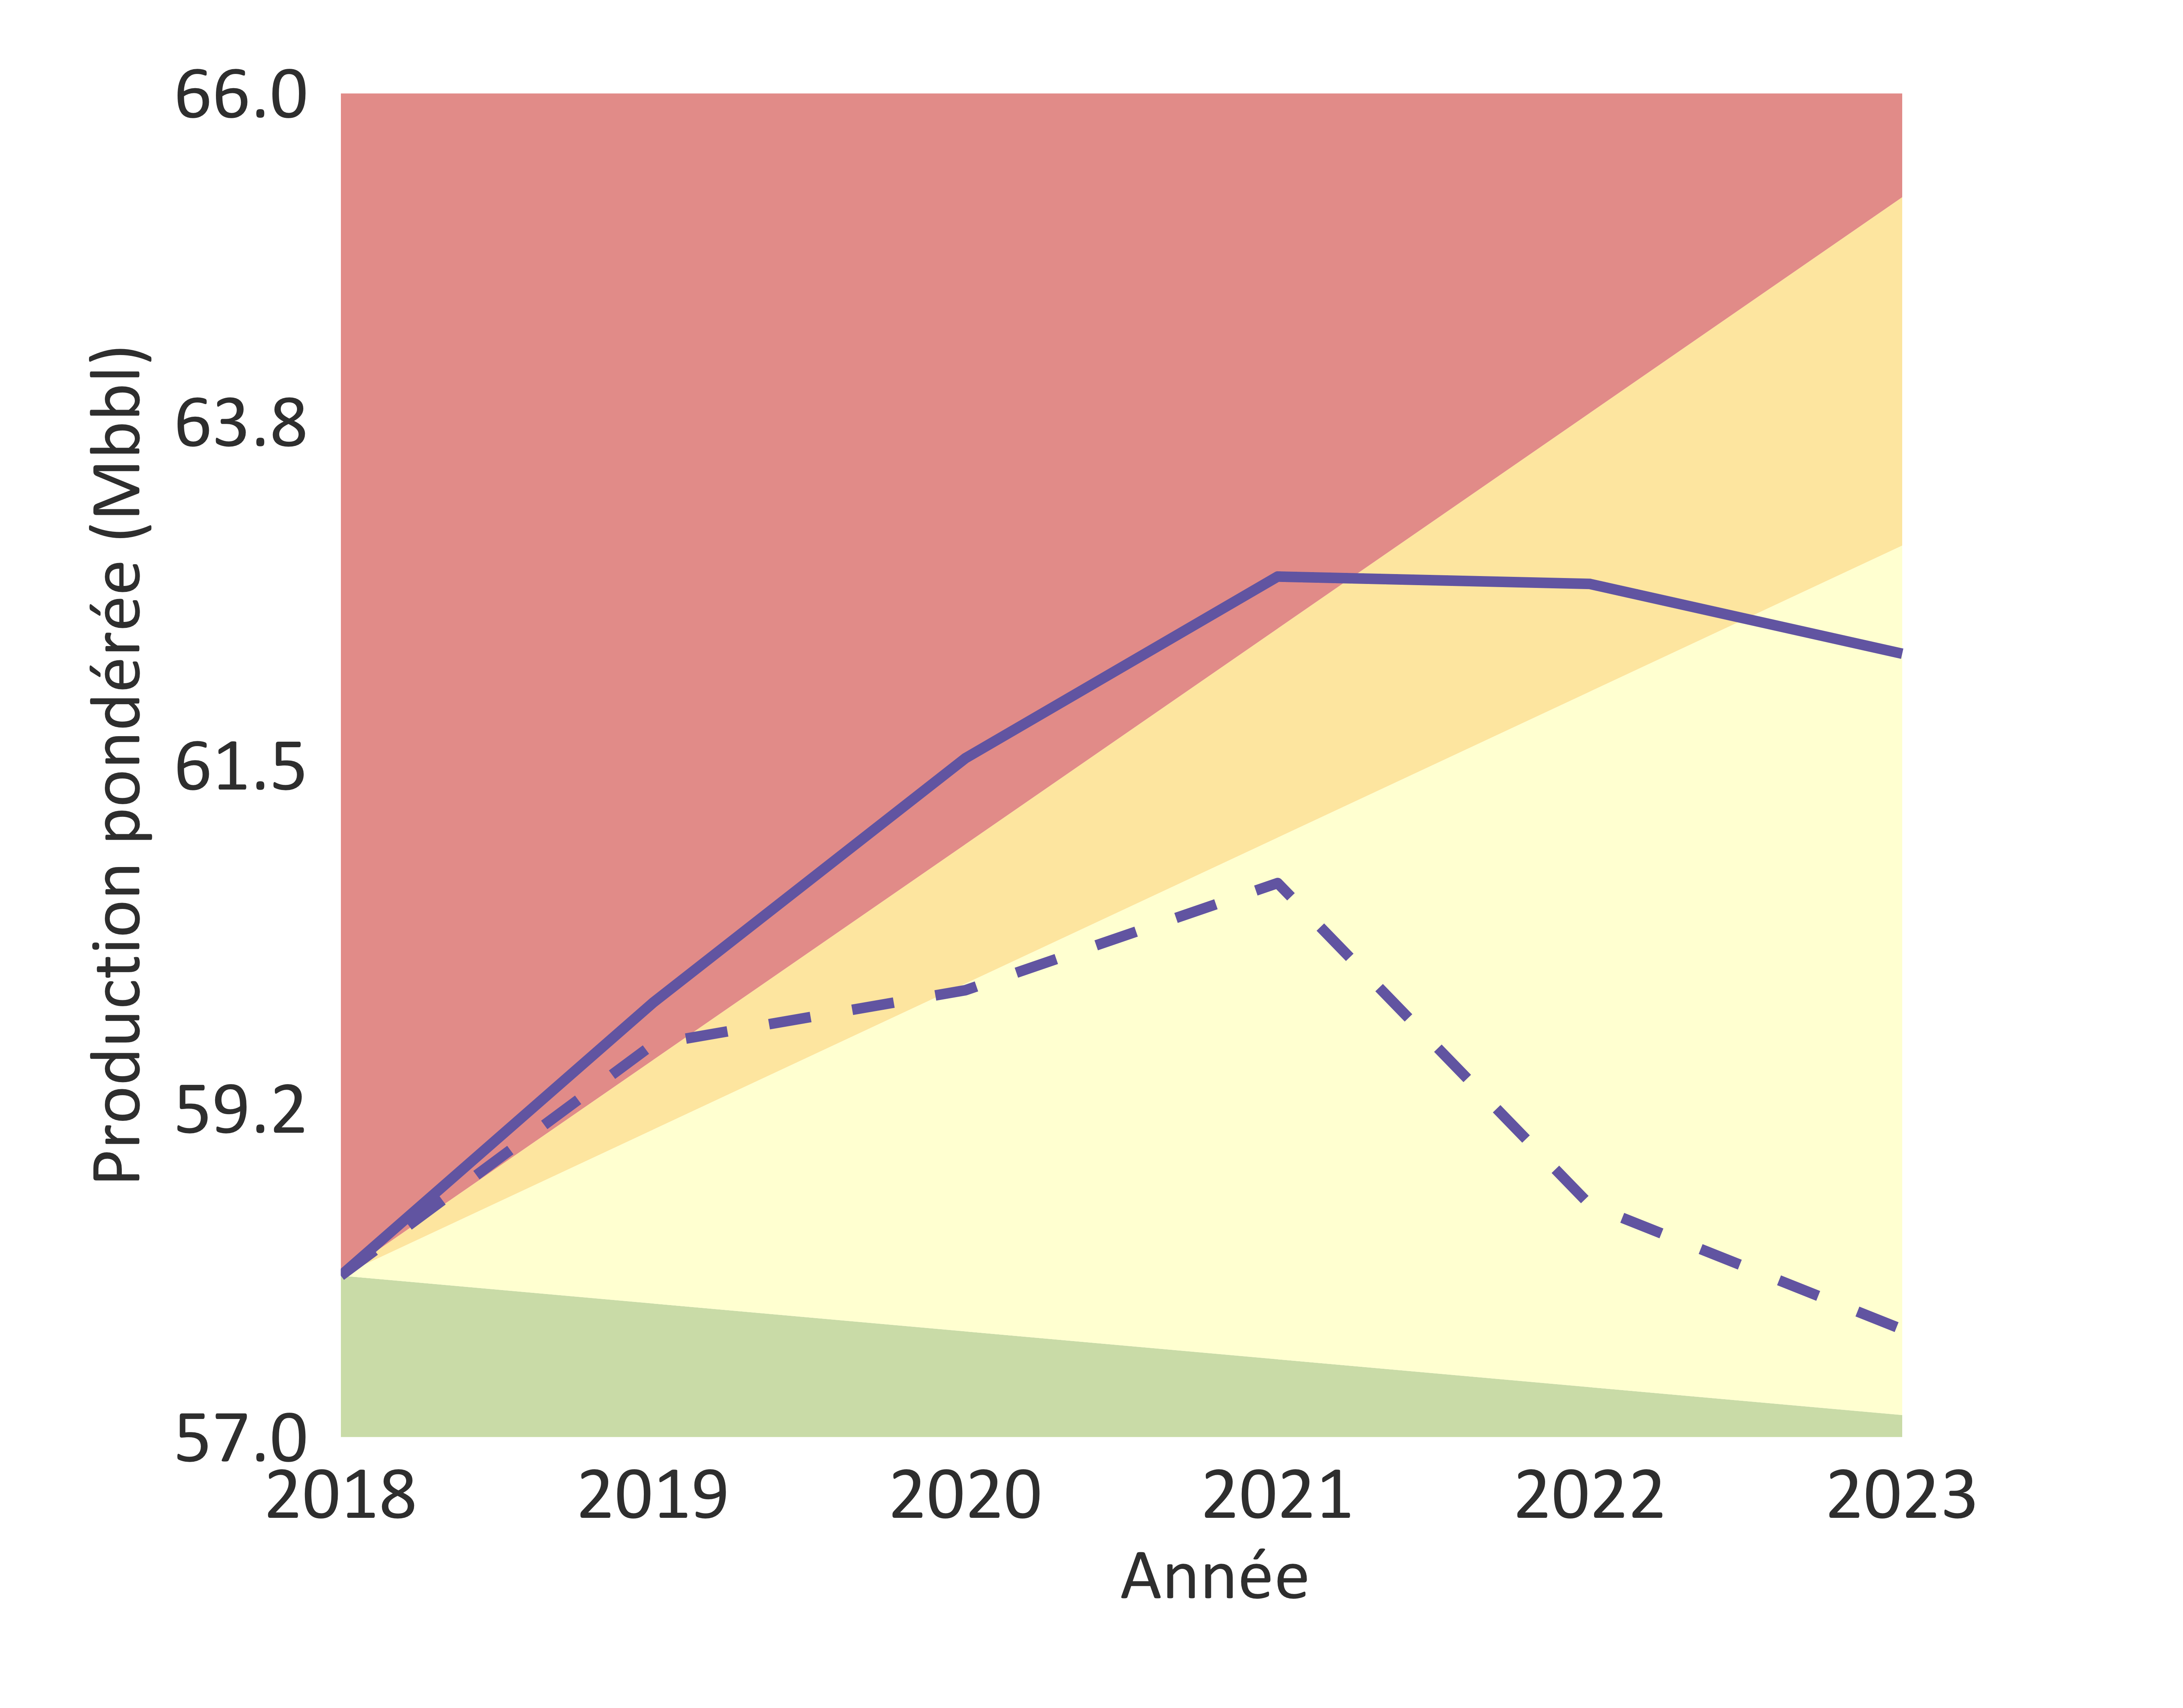
\includegraphics[trim = {0 0cm 0 0},width=1\linewidth]{ReportOutputs/Fig11}
		
	\end{minipage}	
	\hspace{.02\linewidth}
	\begin{minipage}[t]{.49\textwidth}
		\textbf{Trajectory of Gas Production }
		
		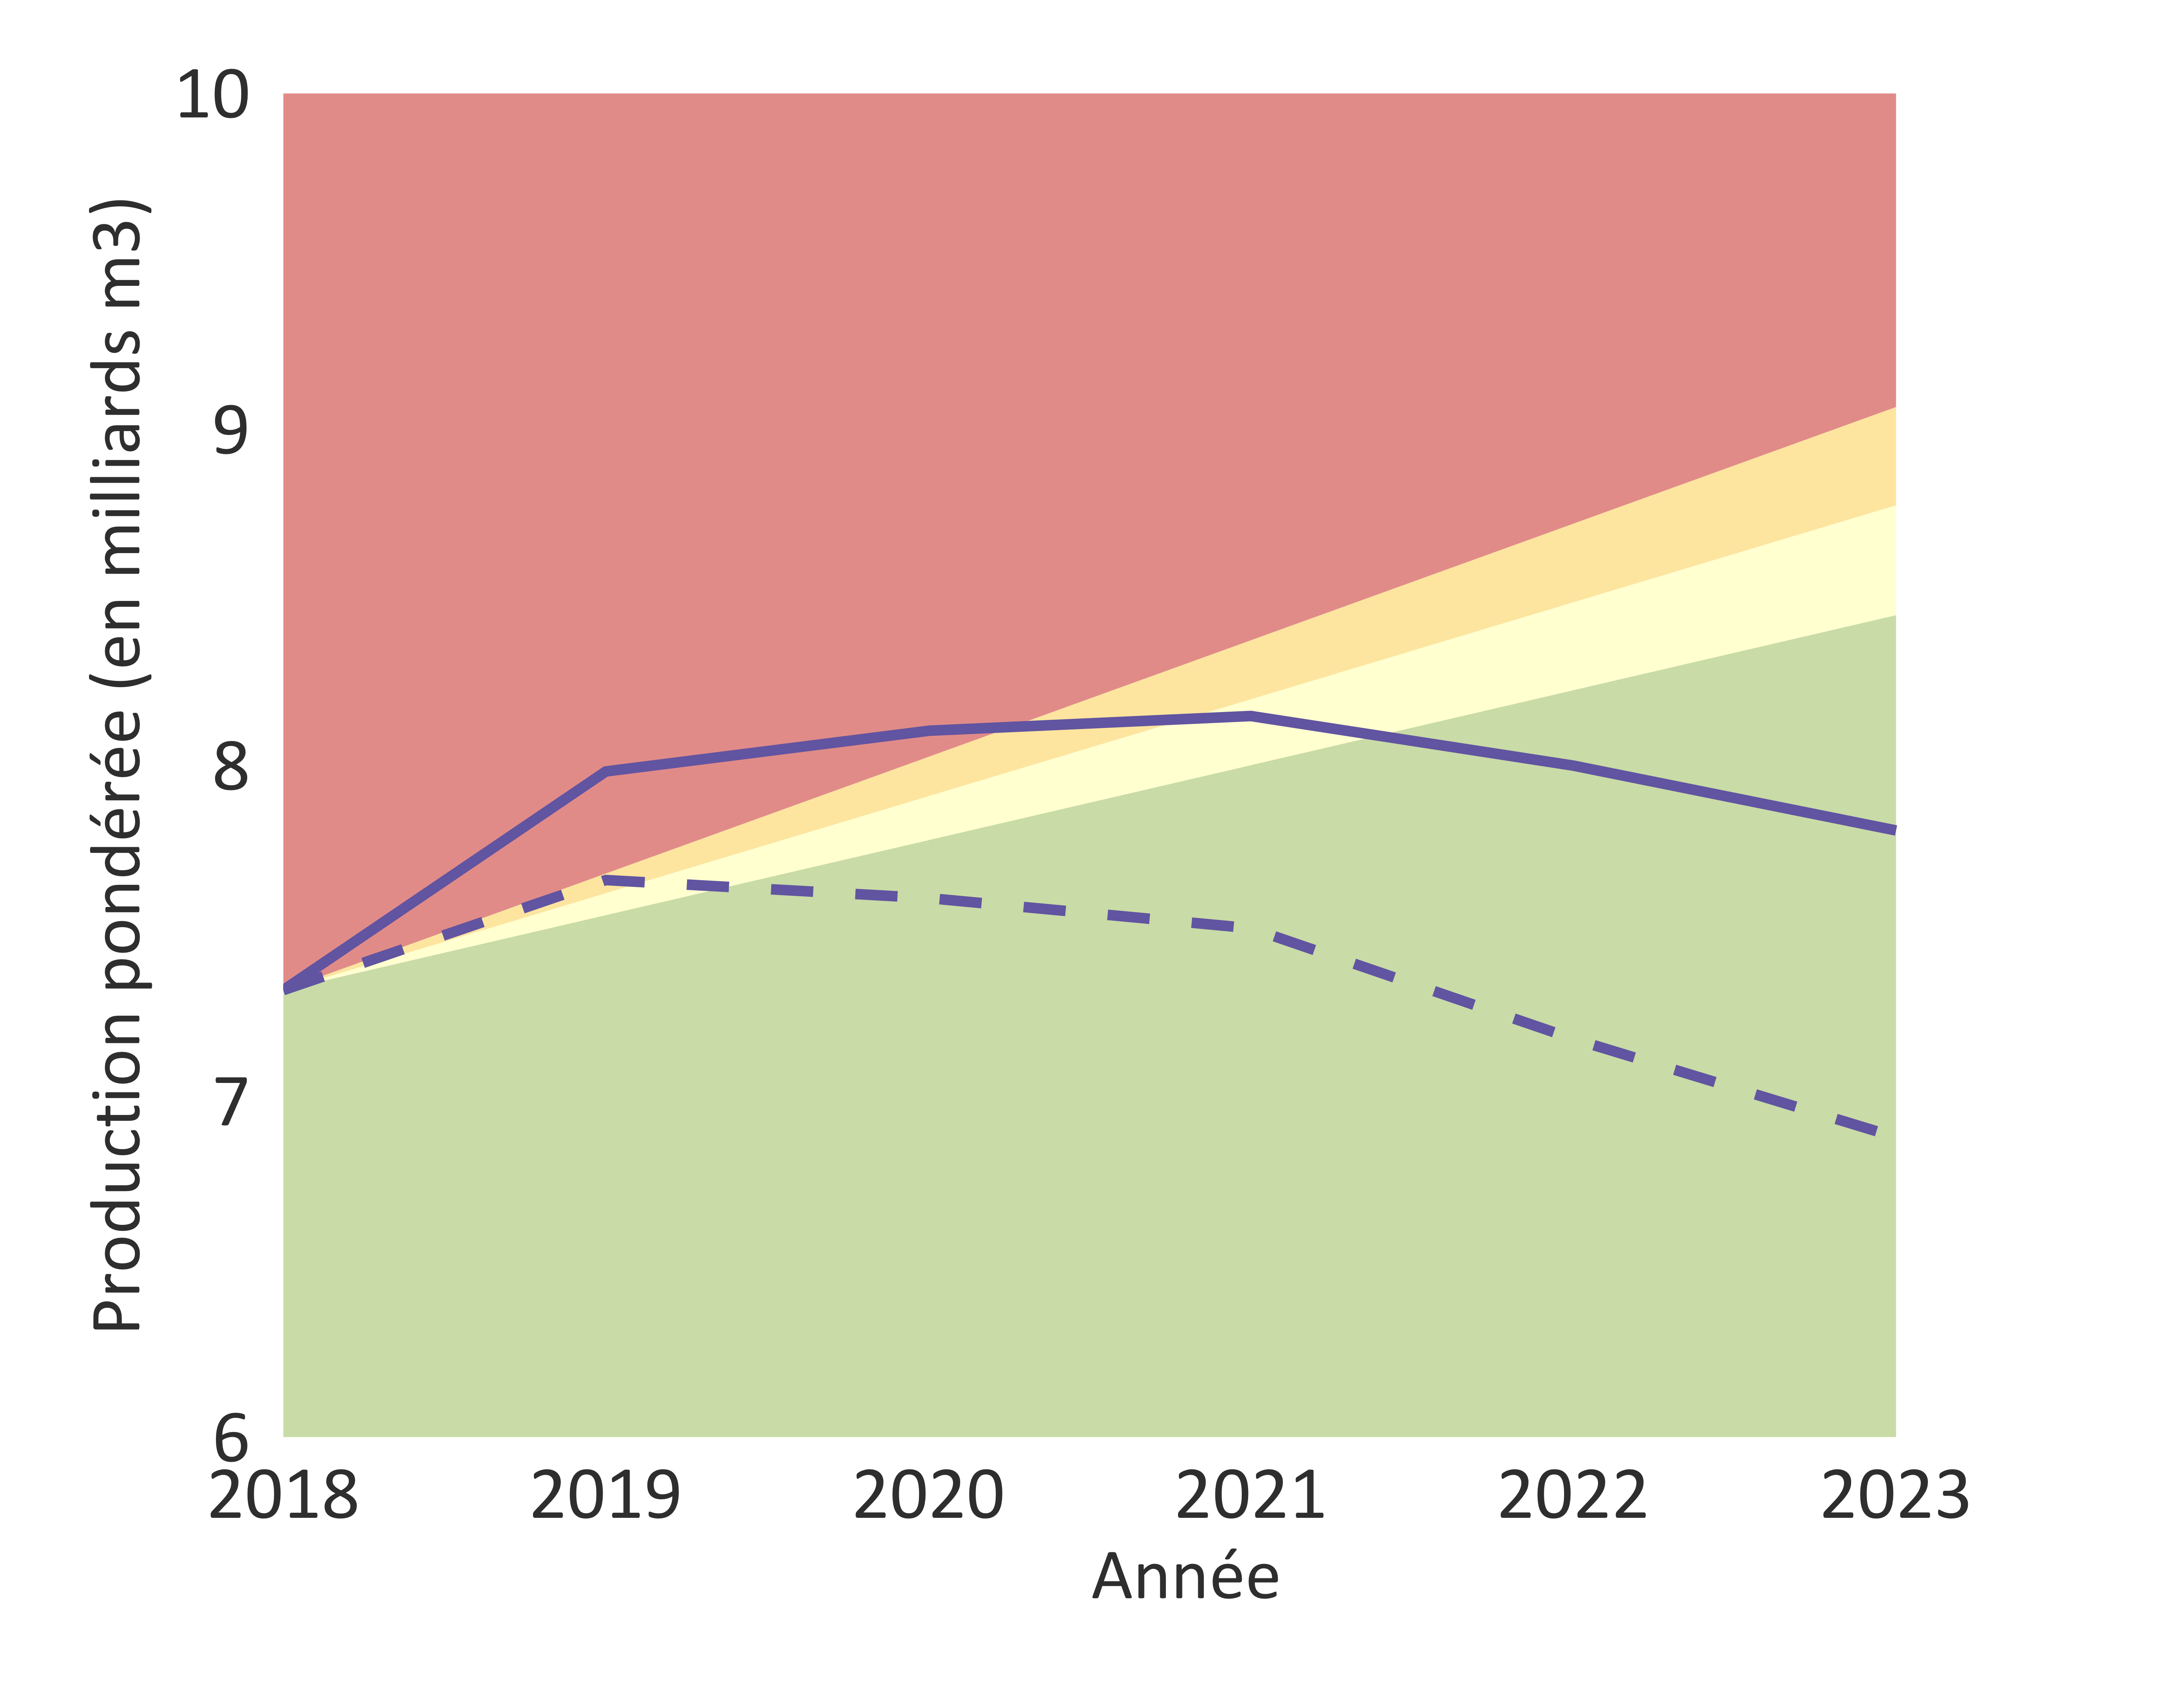
\includegraphics[trim = {0 0cm 0 0},width=1\linewidth]{ReportOutputs/Fig12}
		
	\end{minipage}
	
	

	\begin{minipage}[t]{.49\linewidth}
		\textbf{Trajectory of Coal Production}
		
		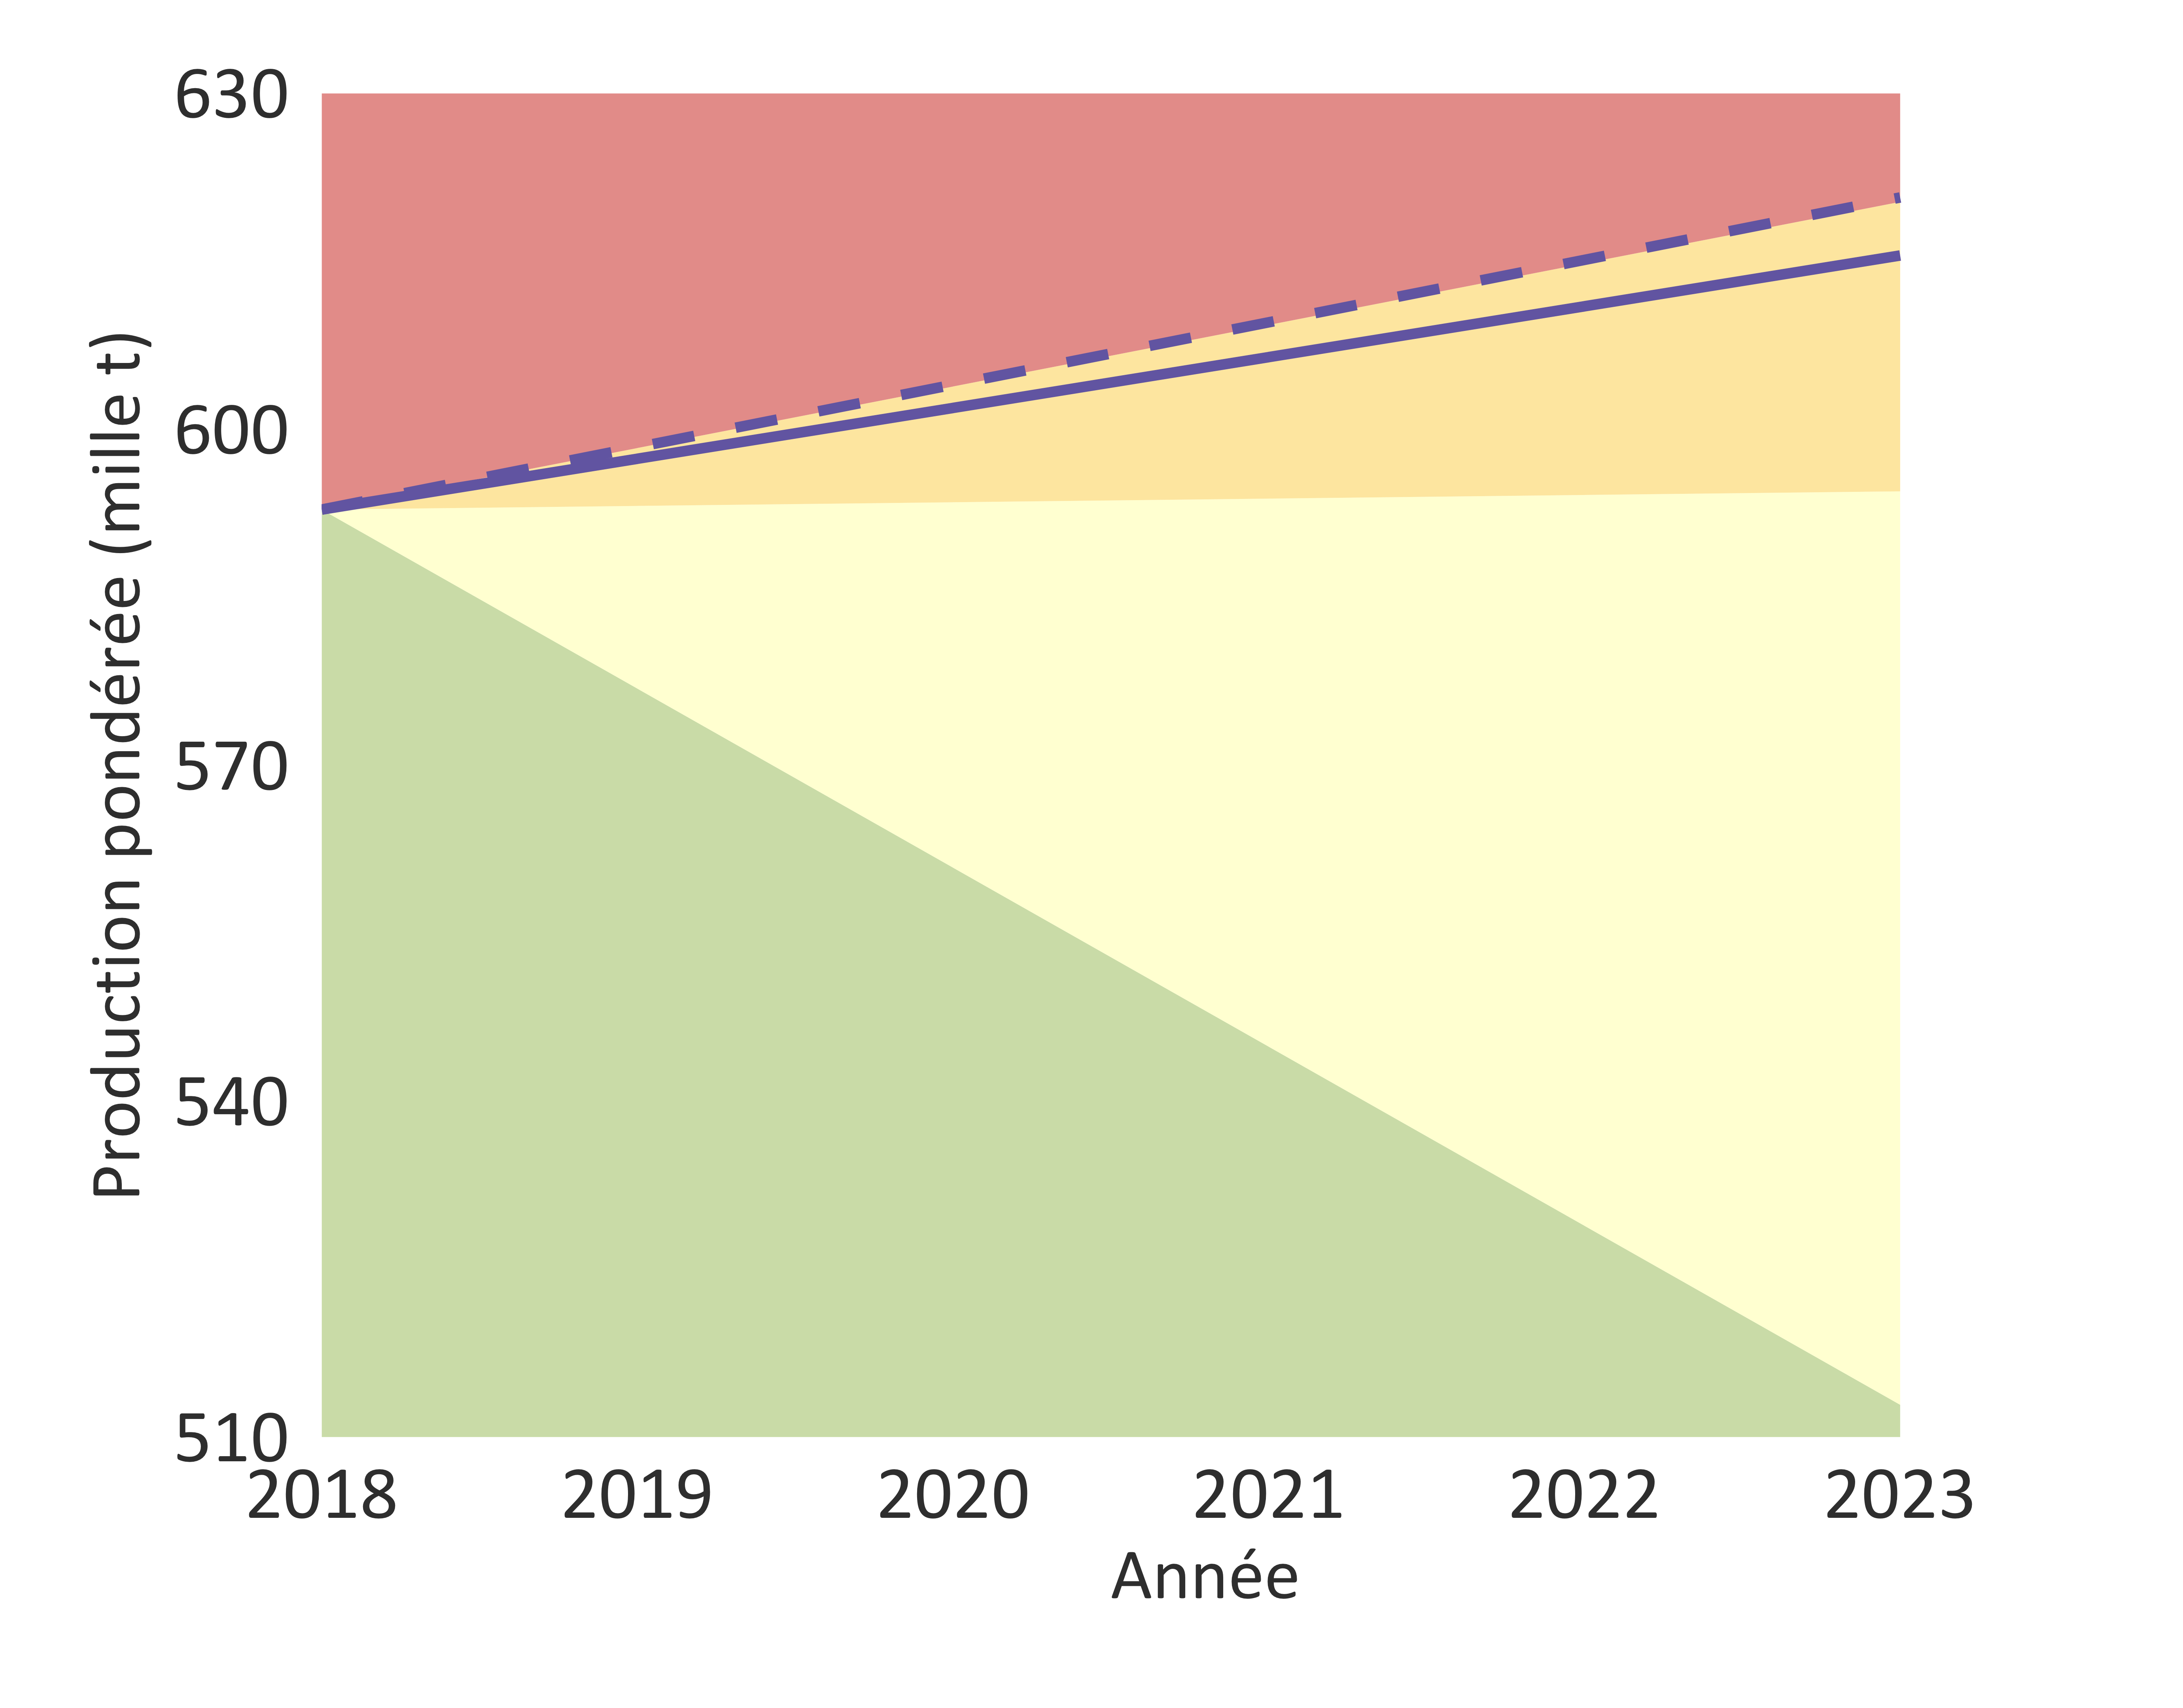
\includegraphics[trim = {0 0cm 0 0},width=1\linewidth]{ReportOutputs/Fig13}
		
	\end{minipage}	
		
	
	\vspace{-.6cm}
	\begin{center}
		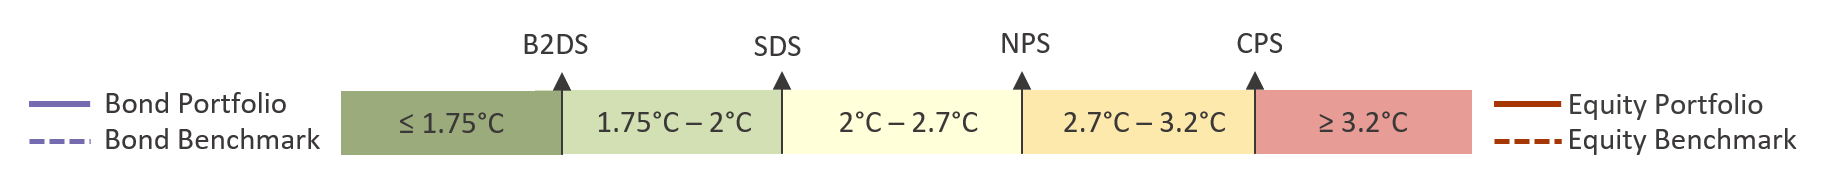
\includegraphics[trim = {0 0cm 0 0},width=.9\linewidth]{ReportGraphics/246Legend.png}
	\end{center}

	
	%\PageFooterThird
\PageFooter{3 - TRAJECTORY OF THE PORTFOLIO}

	\newpage 
	%FossilFuelSector_CBE
	%FossilFuelSector_EQS 
	\section*{} % TRAJECTORY - EQUITY - FOSSIL FUELS AND AUTOMOTIVE  
	\HeaderDouble{5 YEAR TREND - EQUITY}{FOSSIL FUELS}	
	
	\begin{multicols}{2}
		\textbf{The alignment graphs below show the alignment of fossil fuels in the equity portfolio relative to the IEA transition scenarios: B2DS (well below 2°C), SDS (2°C), NPS (4°C), CPS (6°C) and the global corporate bond market. } 
		For each technology, the value plotted for the portfolio (solid line) is the planned evolution or `trajectory' of fossil fuel production allocated to the equity portfolio over the next 5 years. The lines separating the color-coded background areas plot the portfolio's `target production' for each technology under the IEA scenarios. The dotted line shows planned production in the specific technology for the corporate bond market, scaled to the same starting point as the portfolio.                    
		
		
	\end{multicols}		
	
	\begin{center}
		\textbf{Fossil Fuel Sector}
	\end{center}
	
	\begin{minipage}[t]{.49\linewidth}
		\textbf{Trajectory of Oil Production }
		
		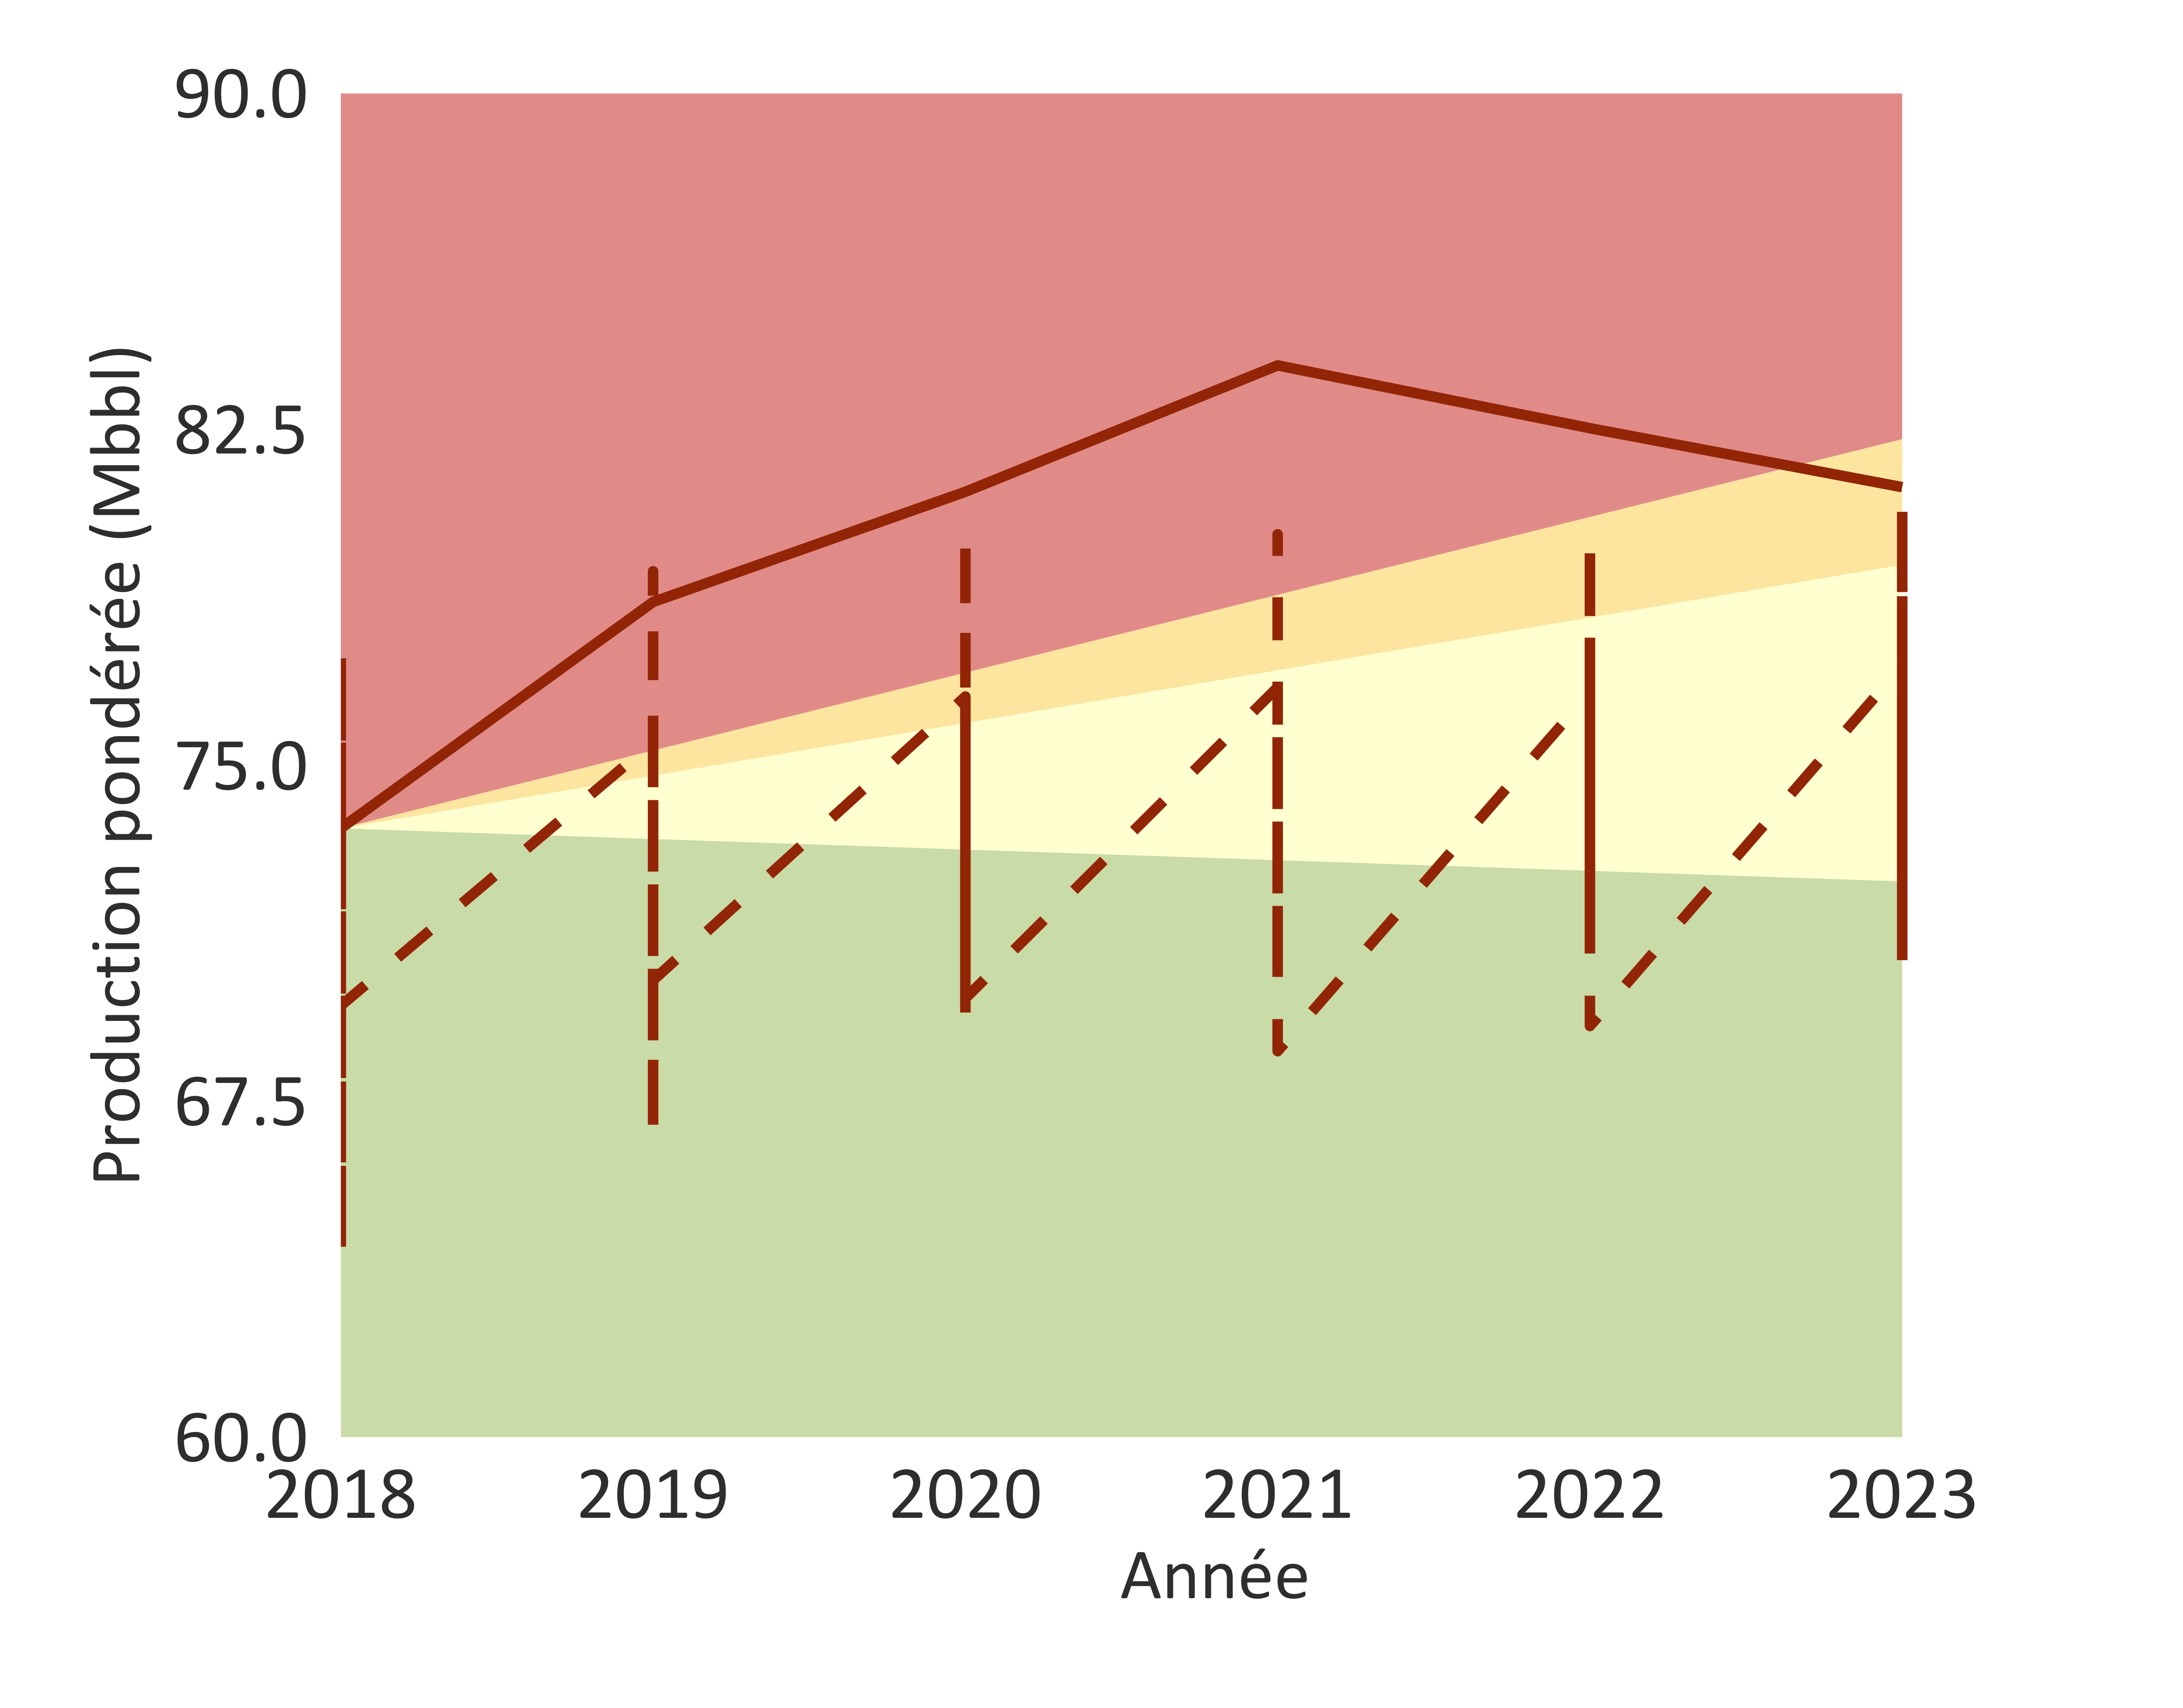
\includegraphics[trim = {0 0cm 0 0},width=1\linewidth]{ReportOutputs/Fig21}
		
	\end{minipage}	
	\hspace{.02\linewidth}
	\begin{minipage}[t]{.49\textwidth}
		\textbf{Trajectory of Gas Production }
		
		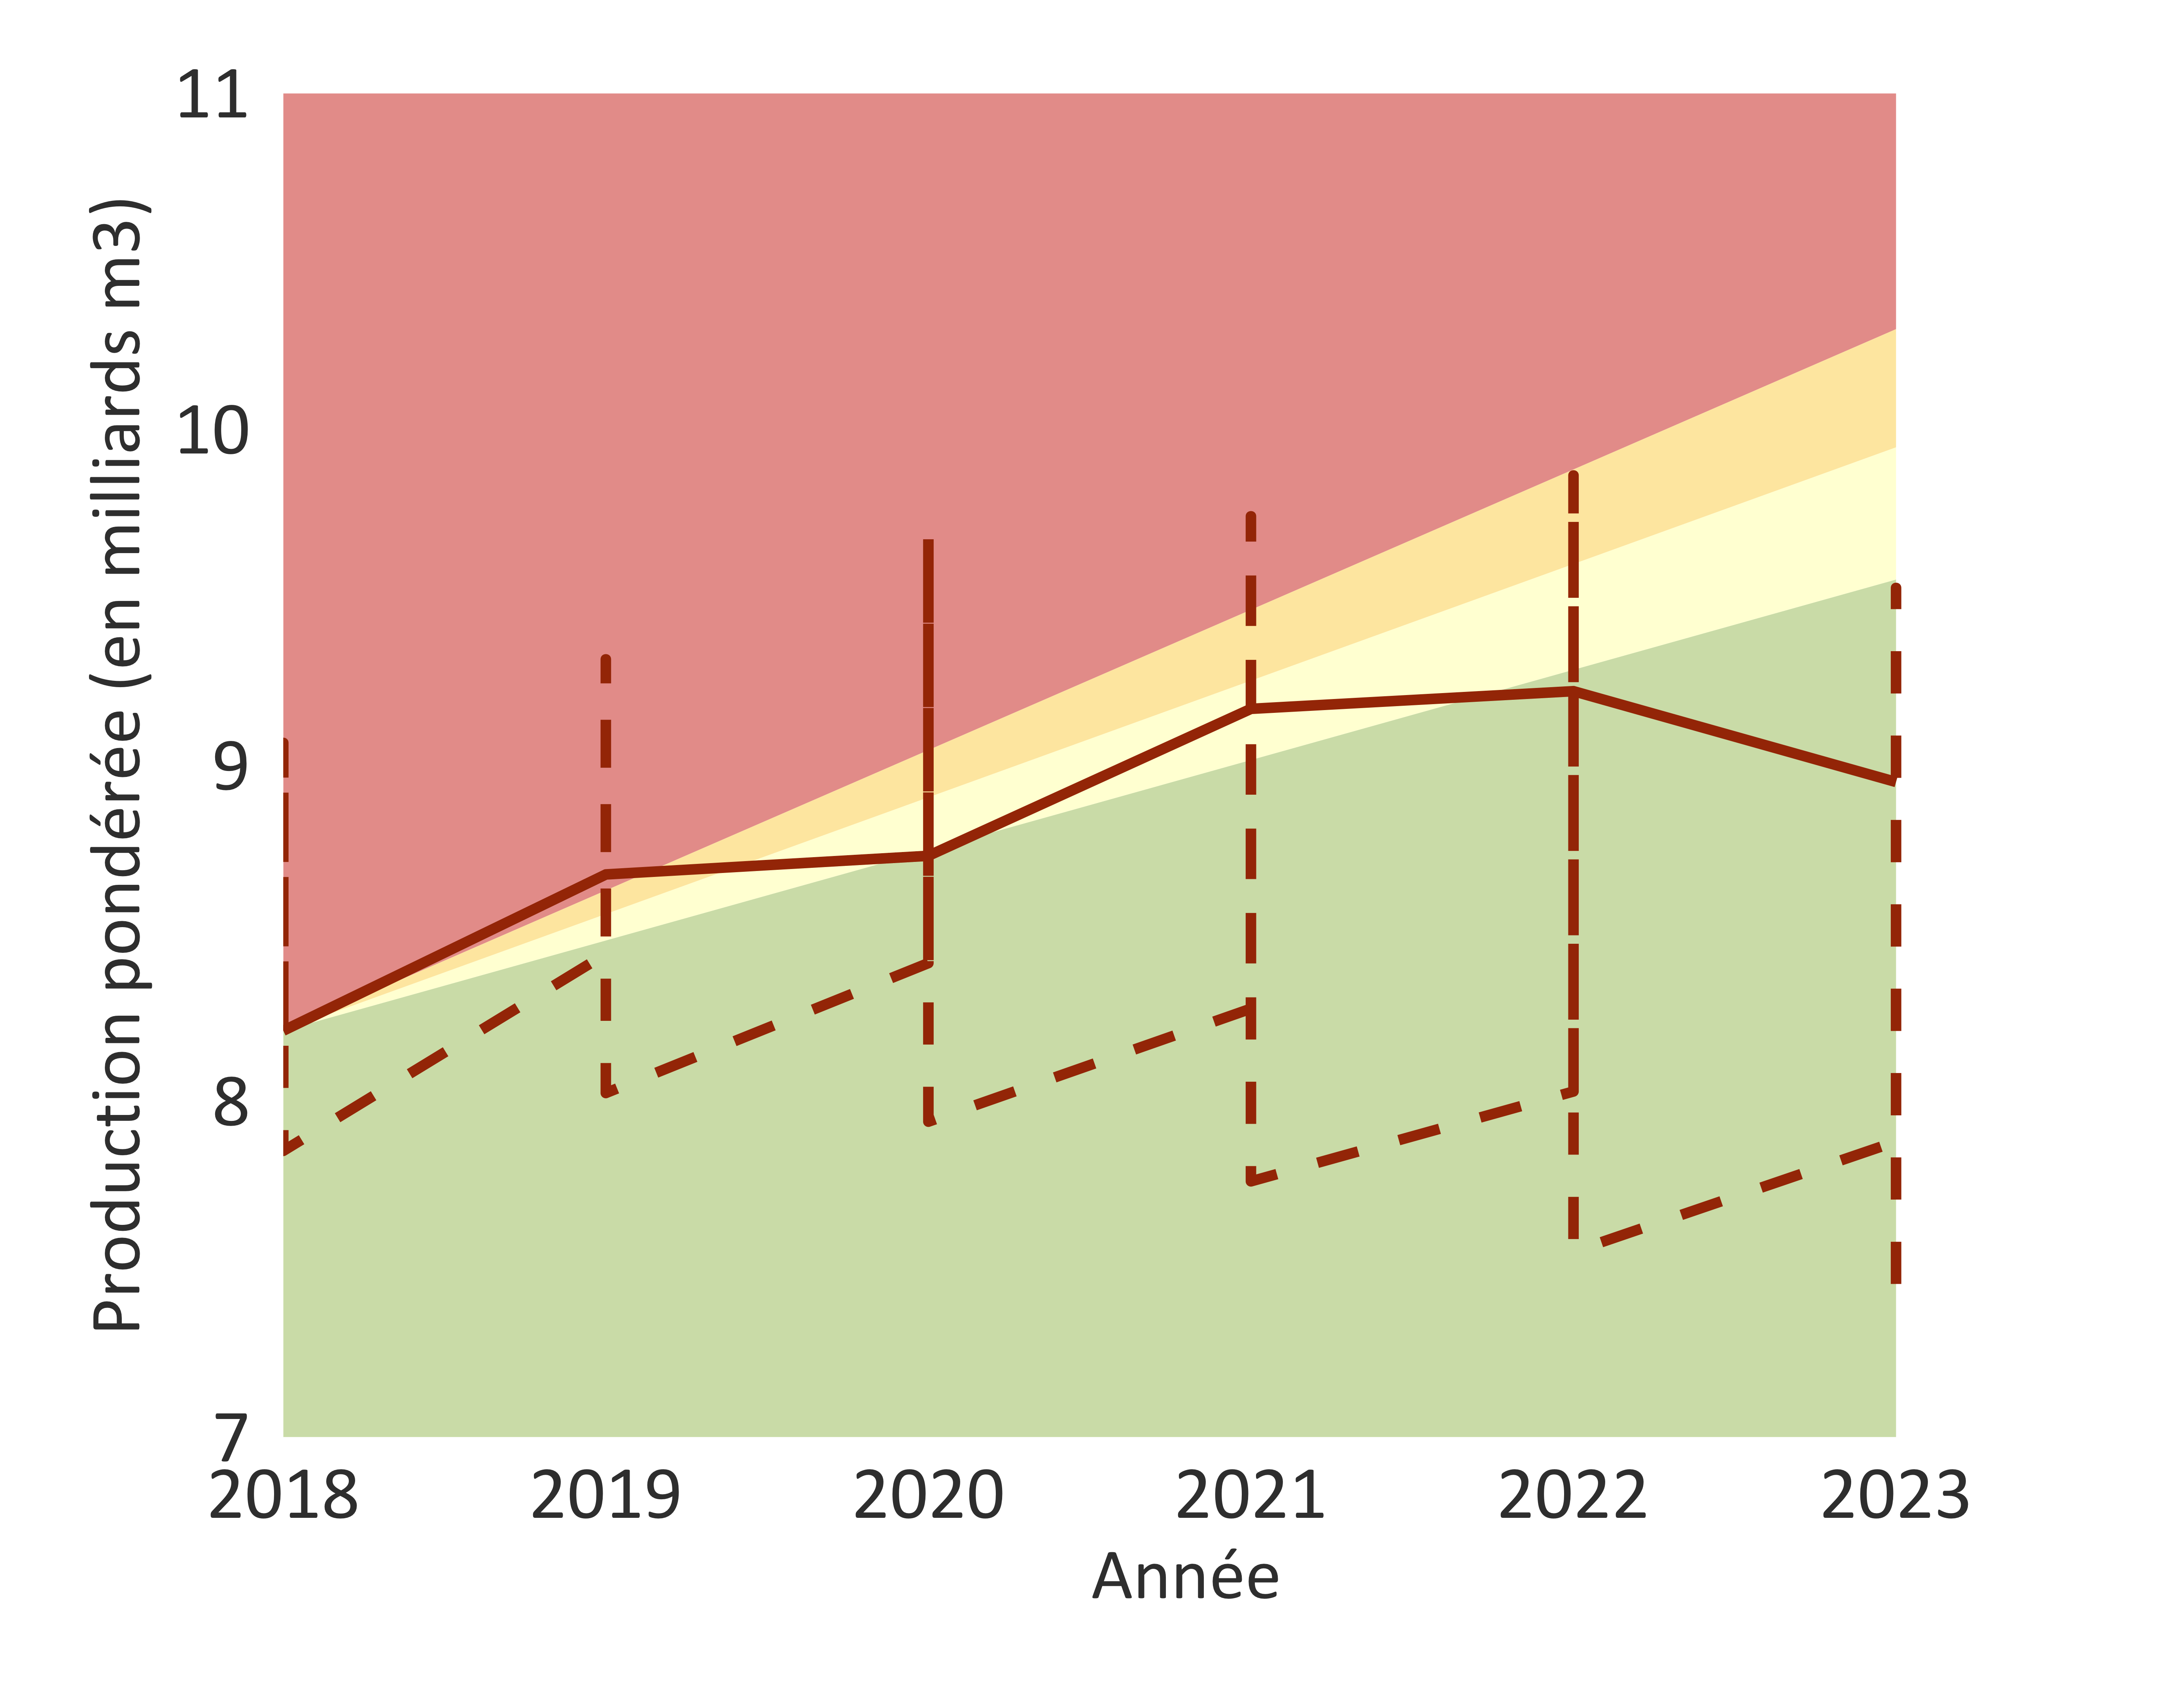
\includegraphics[trim = {0 0cm 0 0},width=1\linewidth]{ReportOutputs/Fig22}
		
	\end{minipage}
	
	
	
	\begin{minipage}[t]{.49\linewidth}
		\textbf{Trajectory of Coal Production}
		
		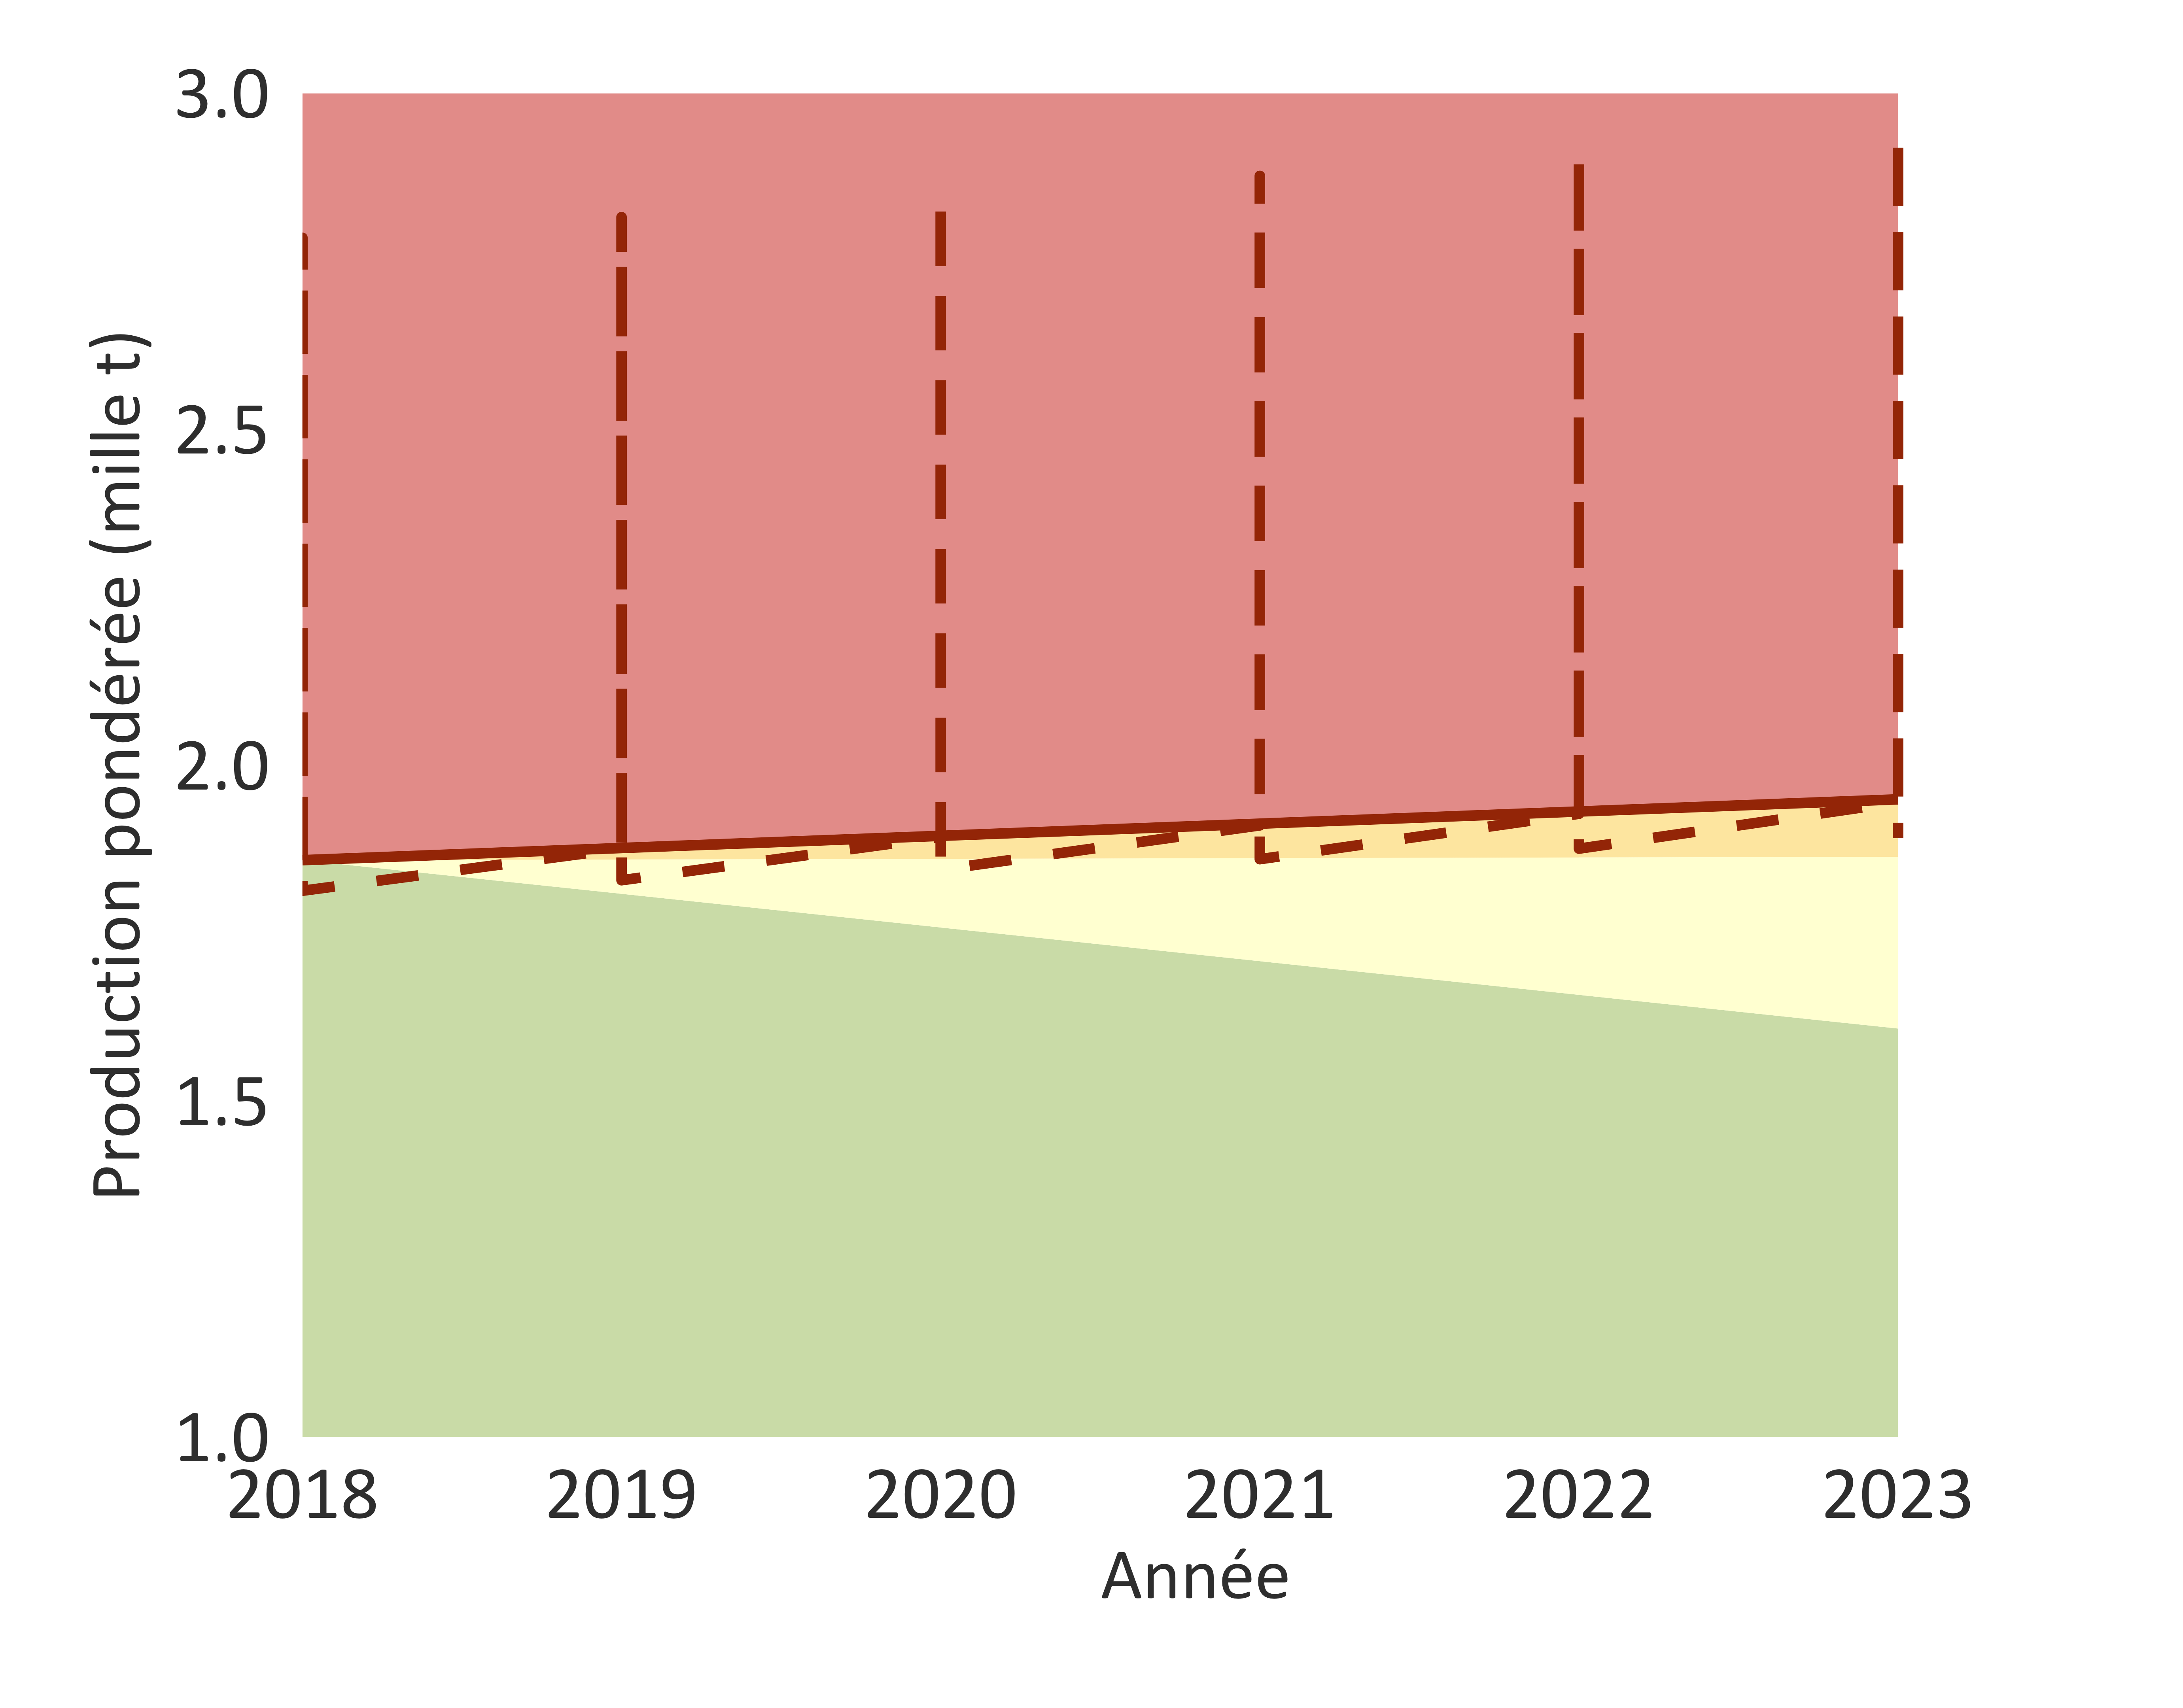
\includegraphics[trim = {0 0cm 0 0},width=1\linewidth]{ReportOutputs/Fig23}
		
	\end{minipage}	
	
	
	\vspace{-.6cm}
	\begin{center}
		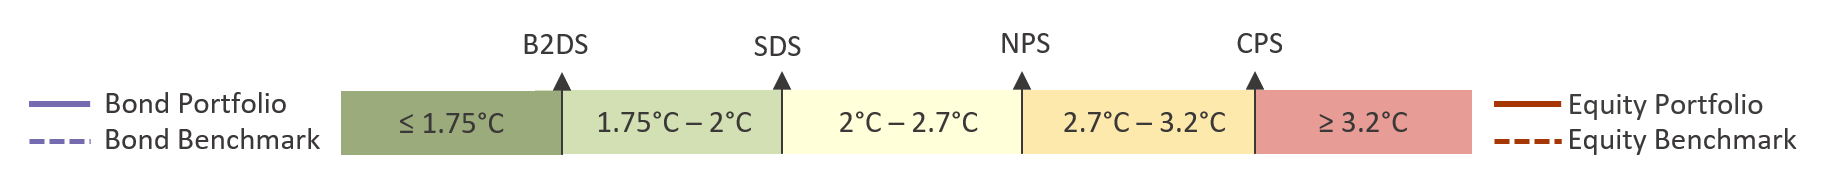
\includegraphics[trim = {0 0cm 0 0},width=.9\linewidth]{ReportGraphics/246Legend.png}
	\end{center}
	
	
	%\PageFooterThird
\PageFooter{3 - TRAJECTORY OF THE PORTFOLIO}
	
	\newpage  
	%FossilFuelSector_EQE 
	%FossilFuelSector_ALLE
	%AutoSector_ALLS
	%AutoSector_CBS
	\section*{} % TRAJECTORY - BONDS - AUTOMOTIVE  
	\HeaderDouble{5 YEAR TREND - CORPORATE BONDS}{AUTOMOTIVE}	
	
	\begin{multicols}{2}
		\textbf{The alignment graphs below show the alignment of automobile technologies in the corporate bond portfolio relative to the IEA scenarios: B2DS (well below 2°C), SDS (2°C), NPS (4°C), CPS (6°C) and the bond market. } 
		For each technology, the value plotted for the portfolio (solid line) is the planned evolution of automobile production allocated to the corporate bond portfolio over the next 5 years.  The lines separating the color-coded background areas plot the portfolio's target production for each technology under the IEA scenarios. The dotted line shows planned production in the specific technology for the bond market, scaled to the same starting point as the portfolio.                    
		
	\end{multicols}		

	
	\begin{minipage}[t]{.49\linewidth}
		\textbf{Trajectory of ICE Vehicle Production}
		
		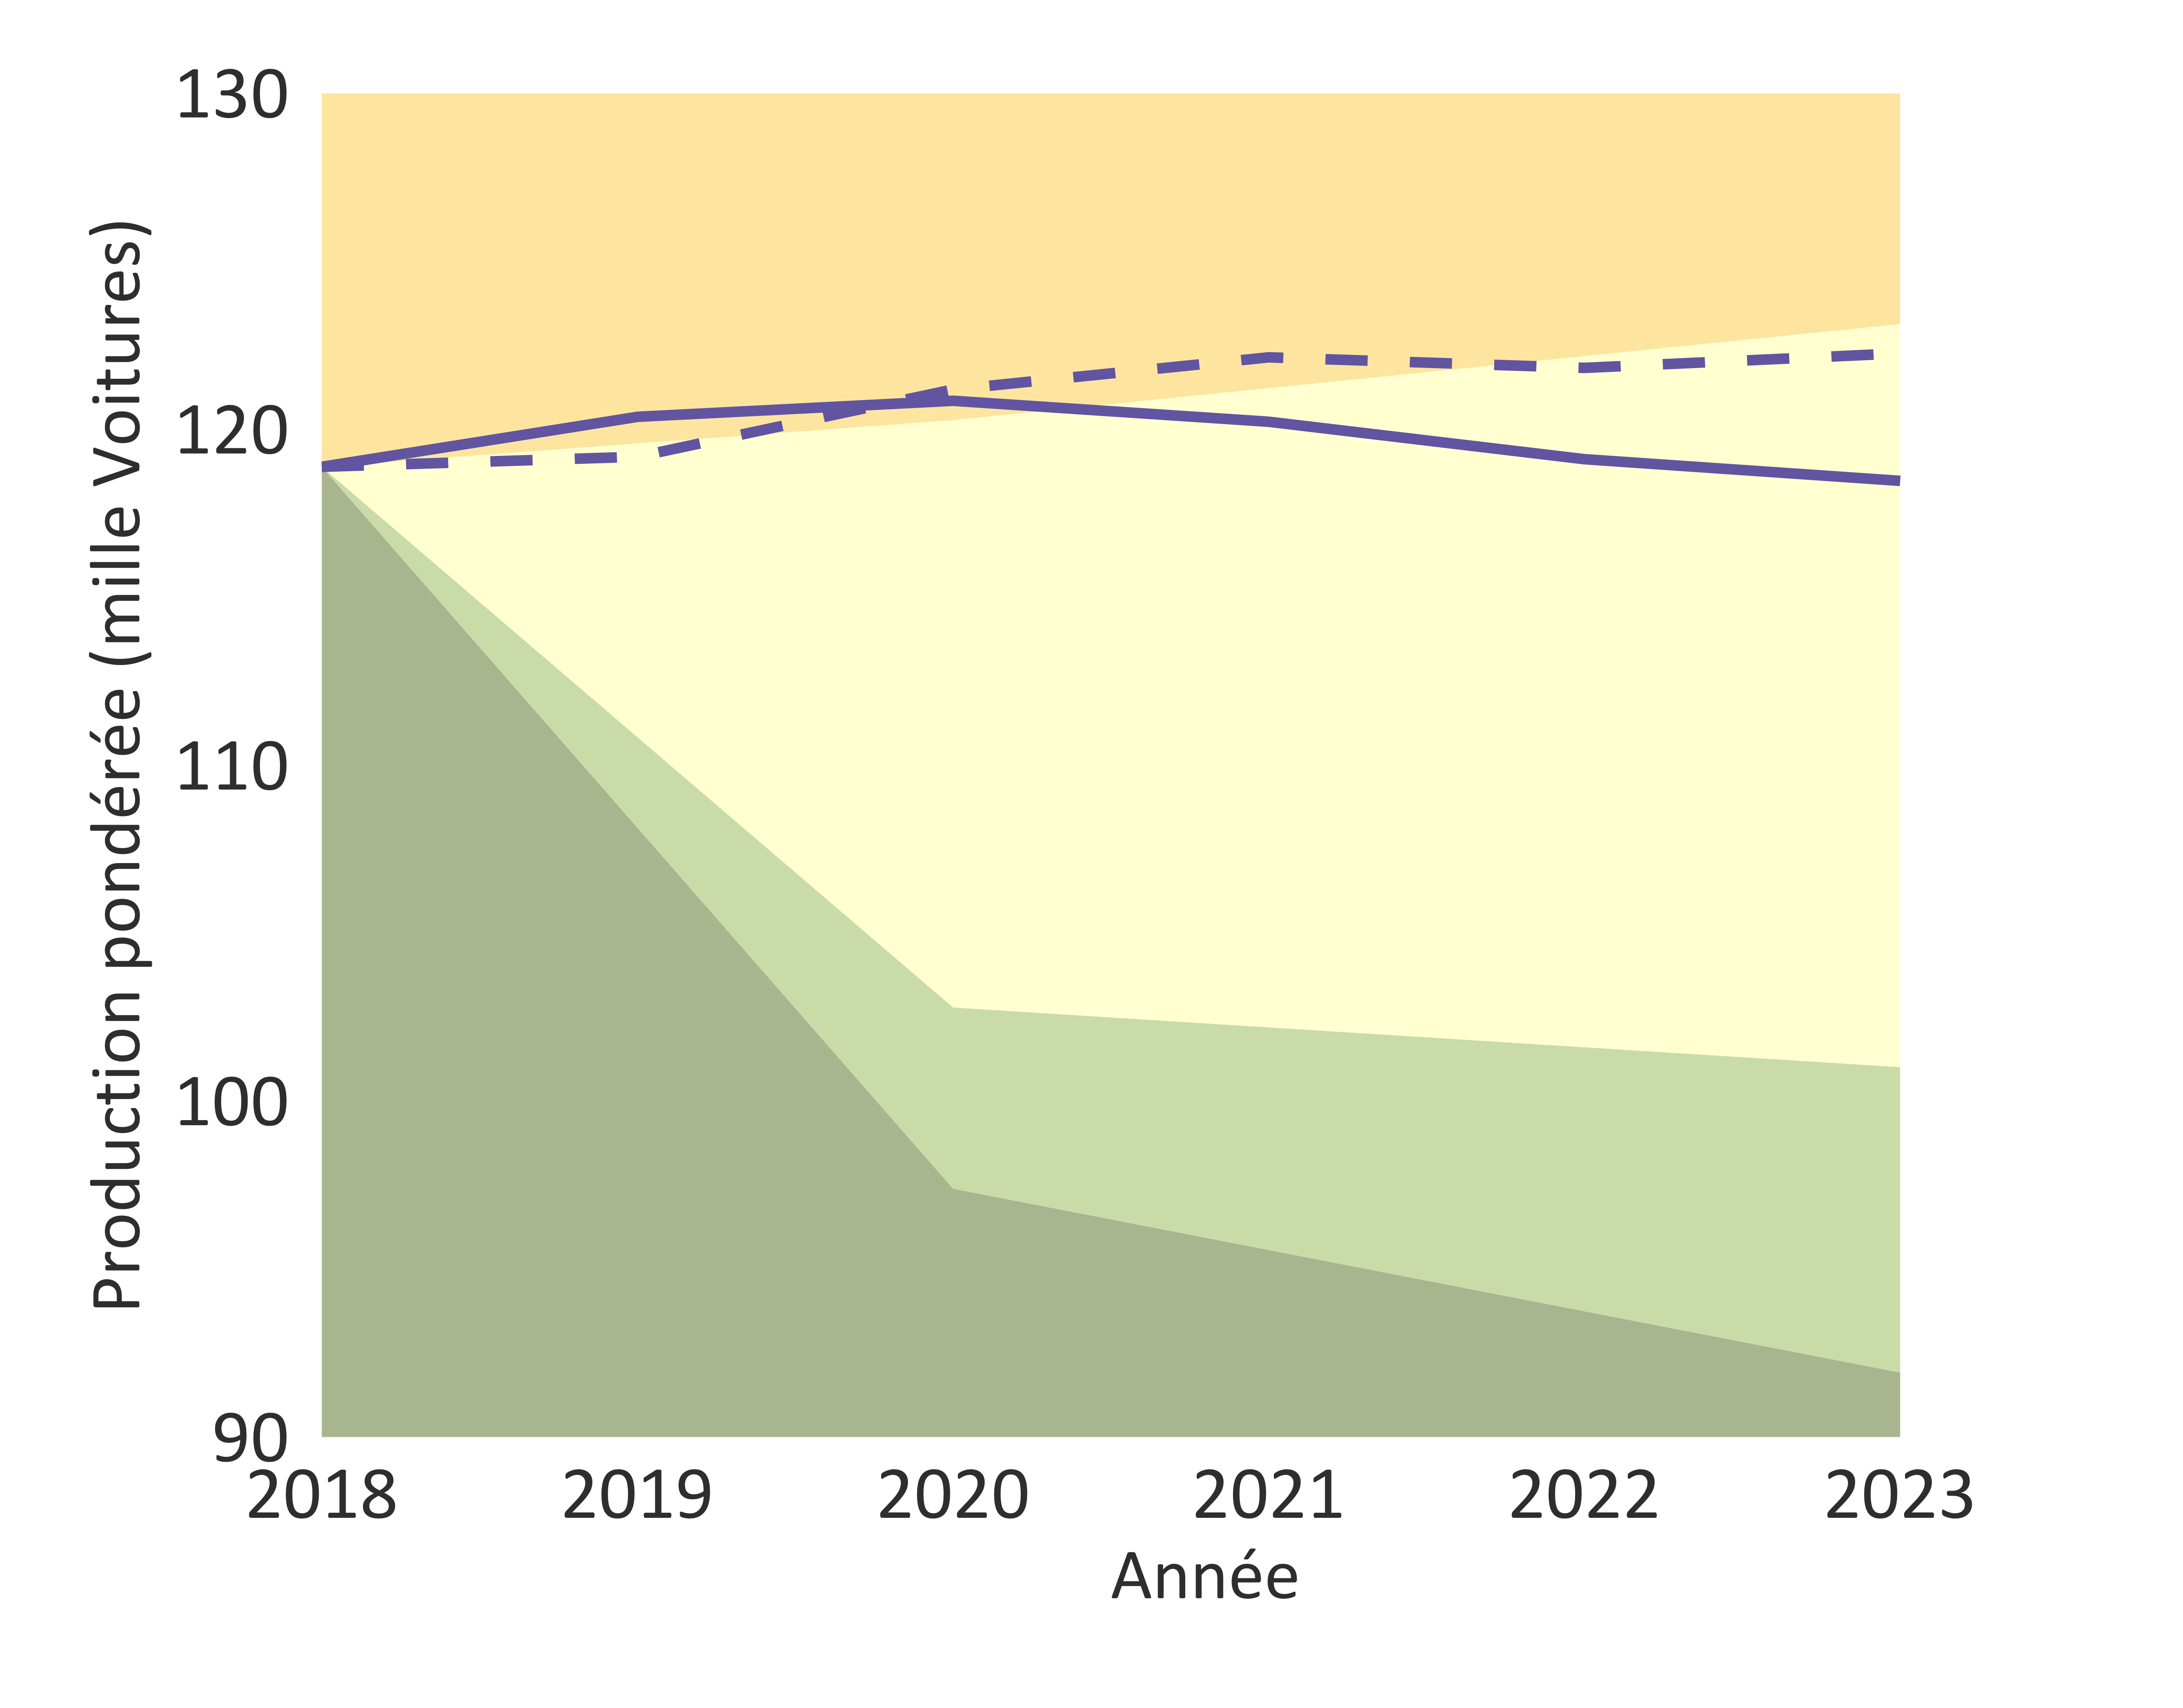
\includegraphics[trim = {0 0cm 0 0},width=1\linewidth]{ReportOutputs/Fig14}
		
	\end{minipage}	
	\hspace{.02\linewidth}
	\begin{minipage}[t]{.49\textwidth}
		\textbf{Trajectory of Electric Vehicle Production}
		
		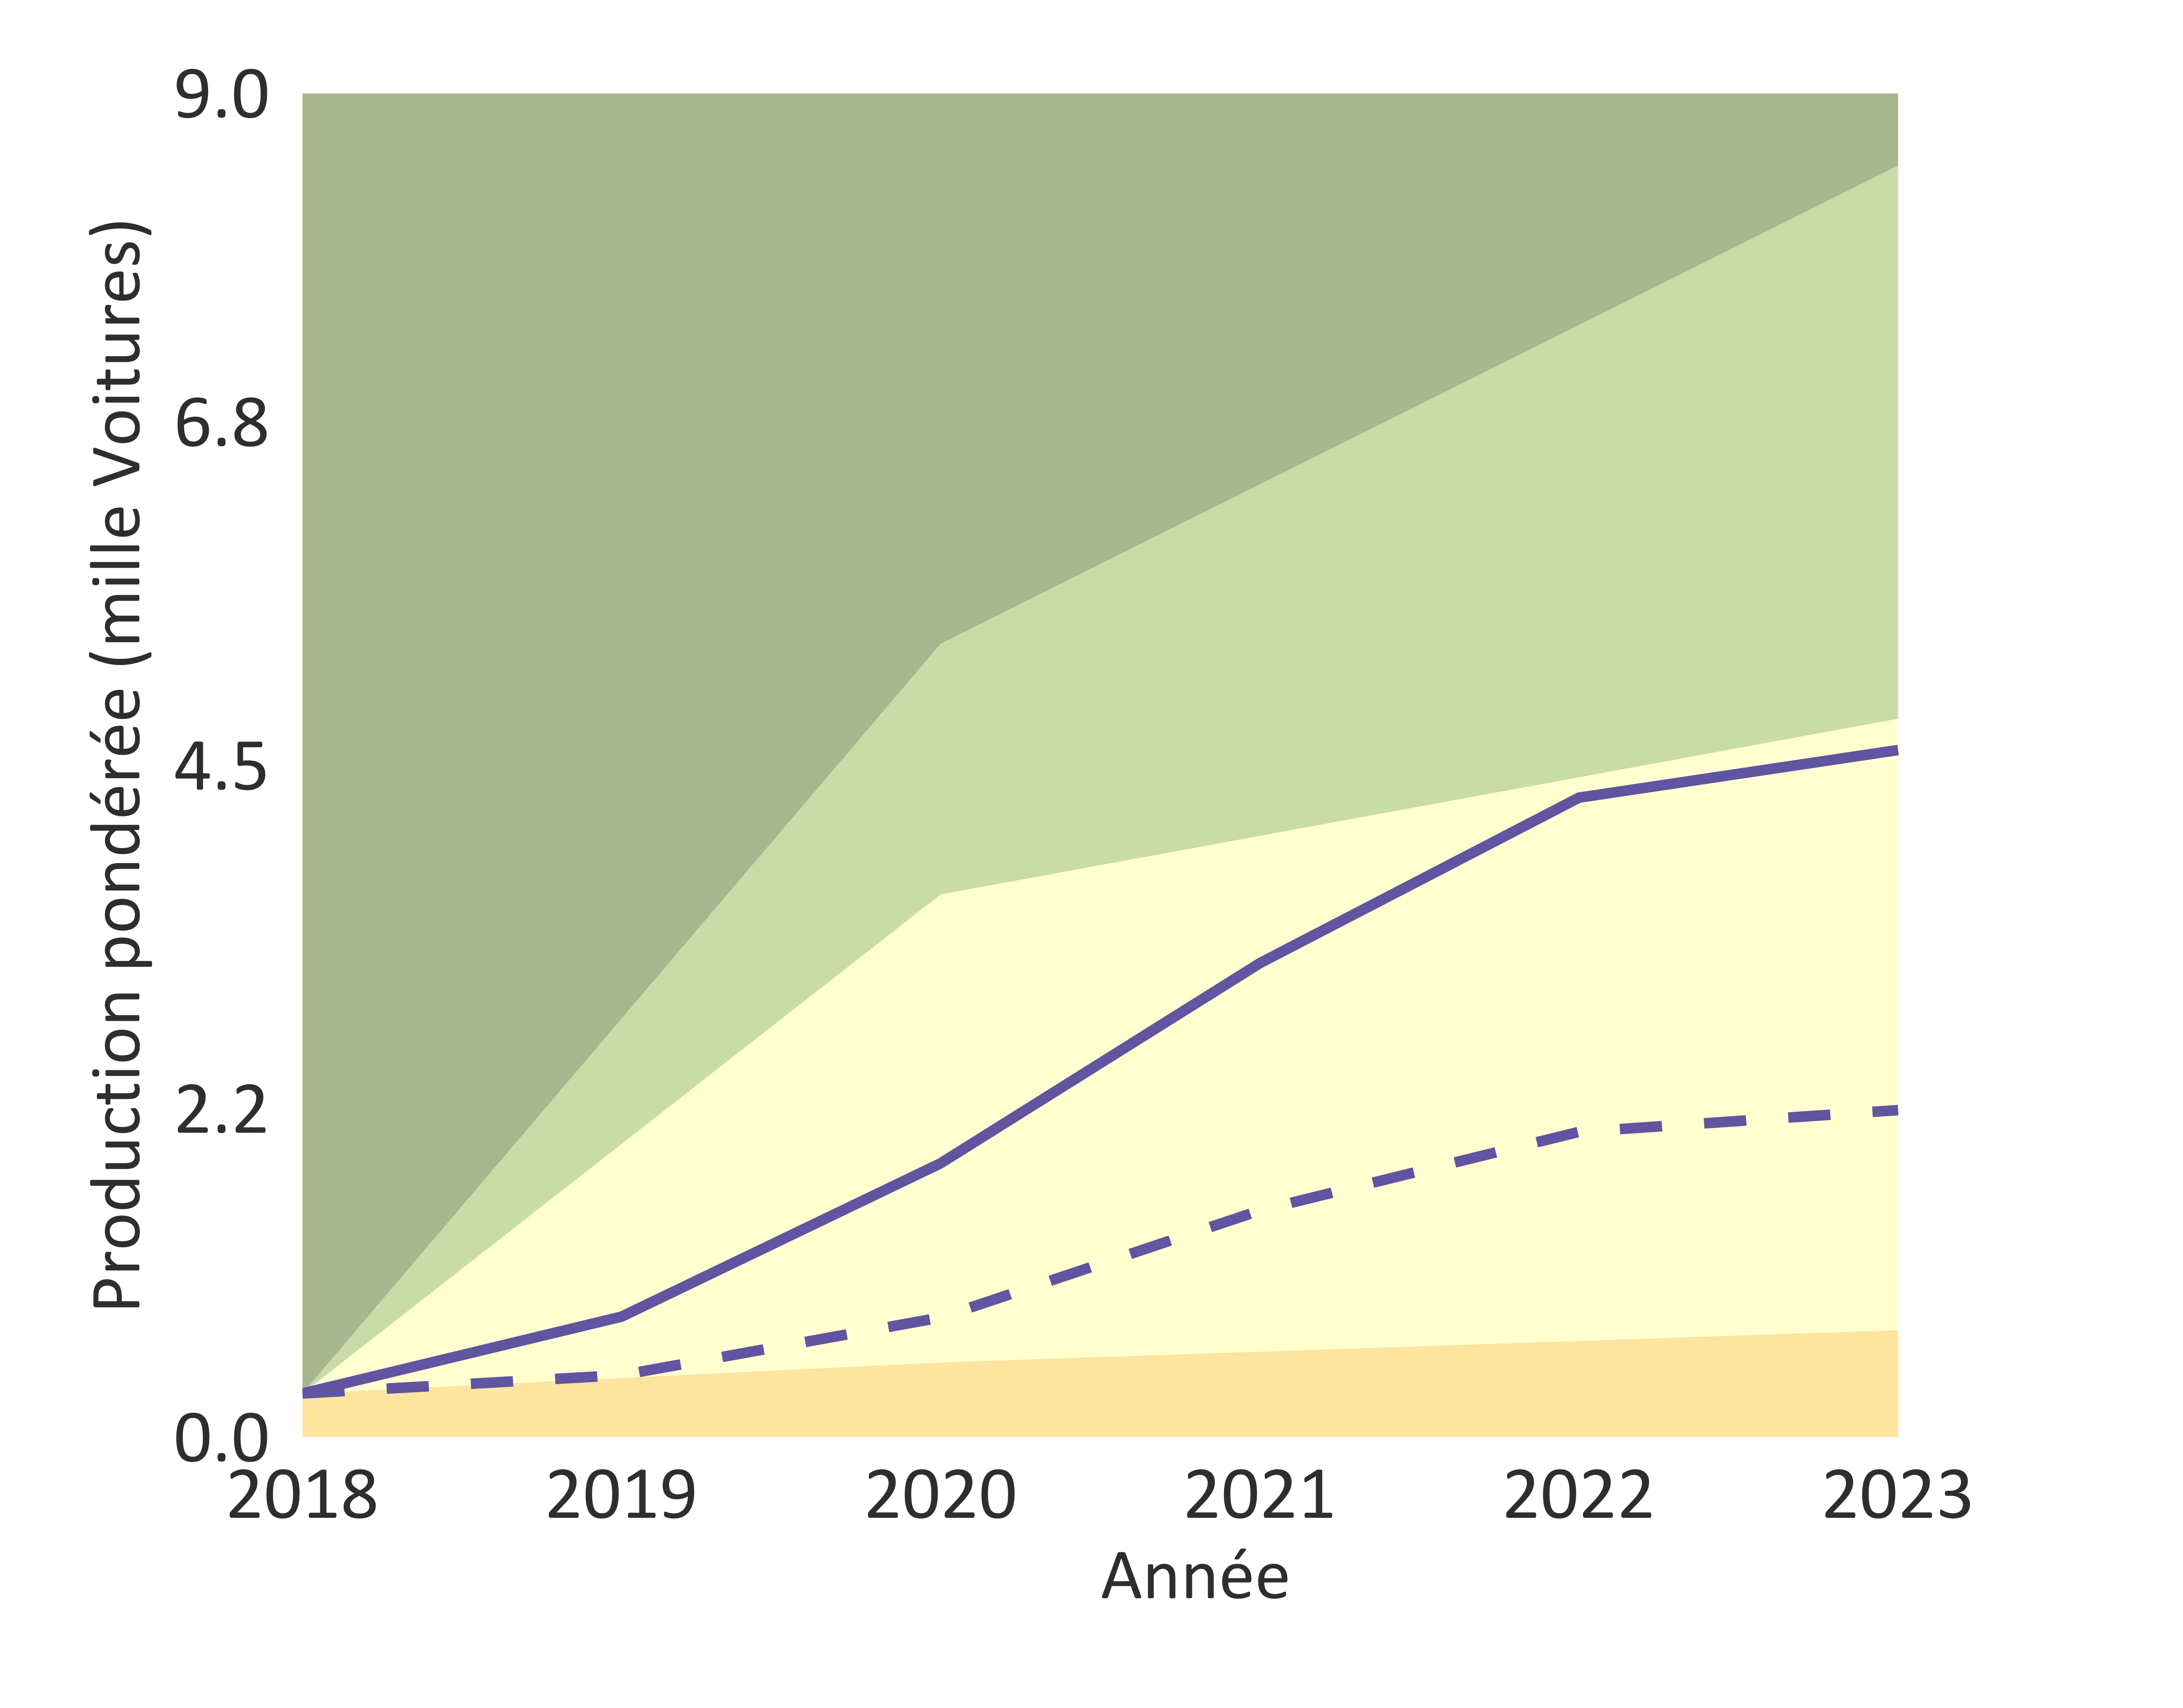
\includegraphics[trim = {0 0cm 0 0},width=1\linewidth]{ReportOutputs/Fig15}
		
	\end{minipage}	

	\begin{minipage}[t]{.49\textwidth}
		\textbf{Trajectory of Hybrid Vehicle Production}
	
		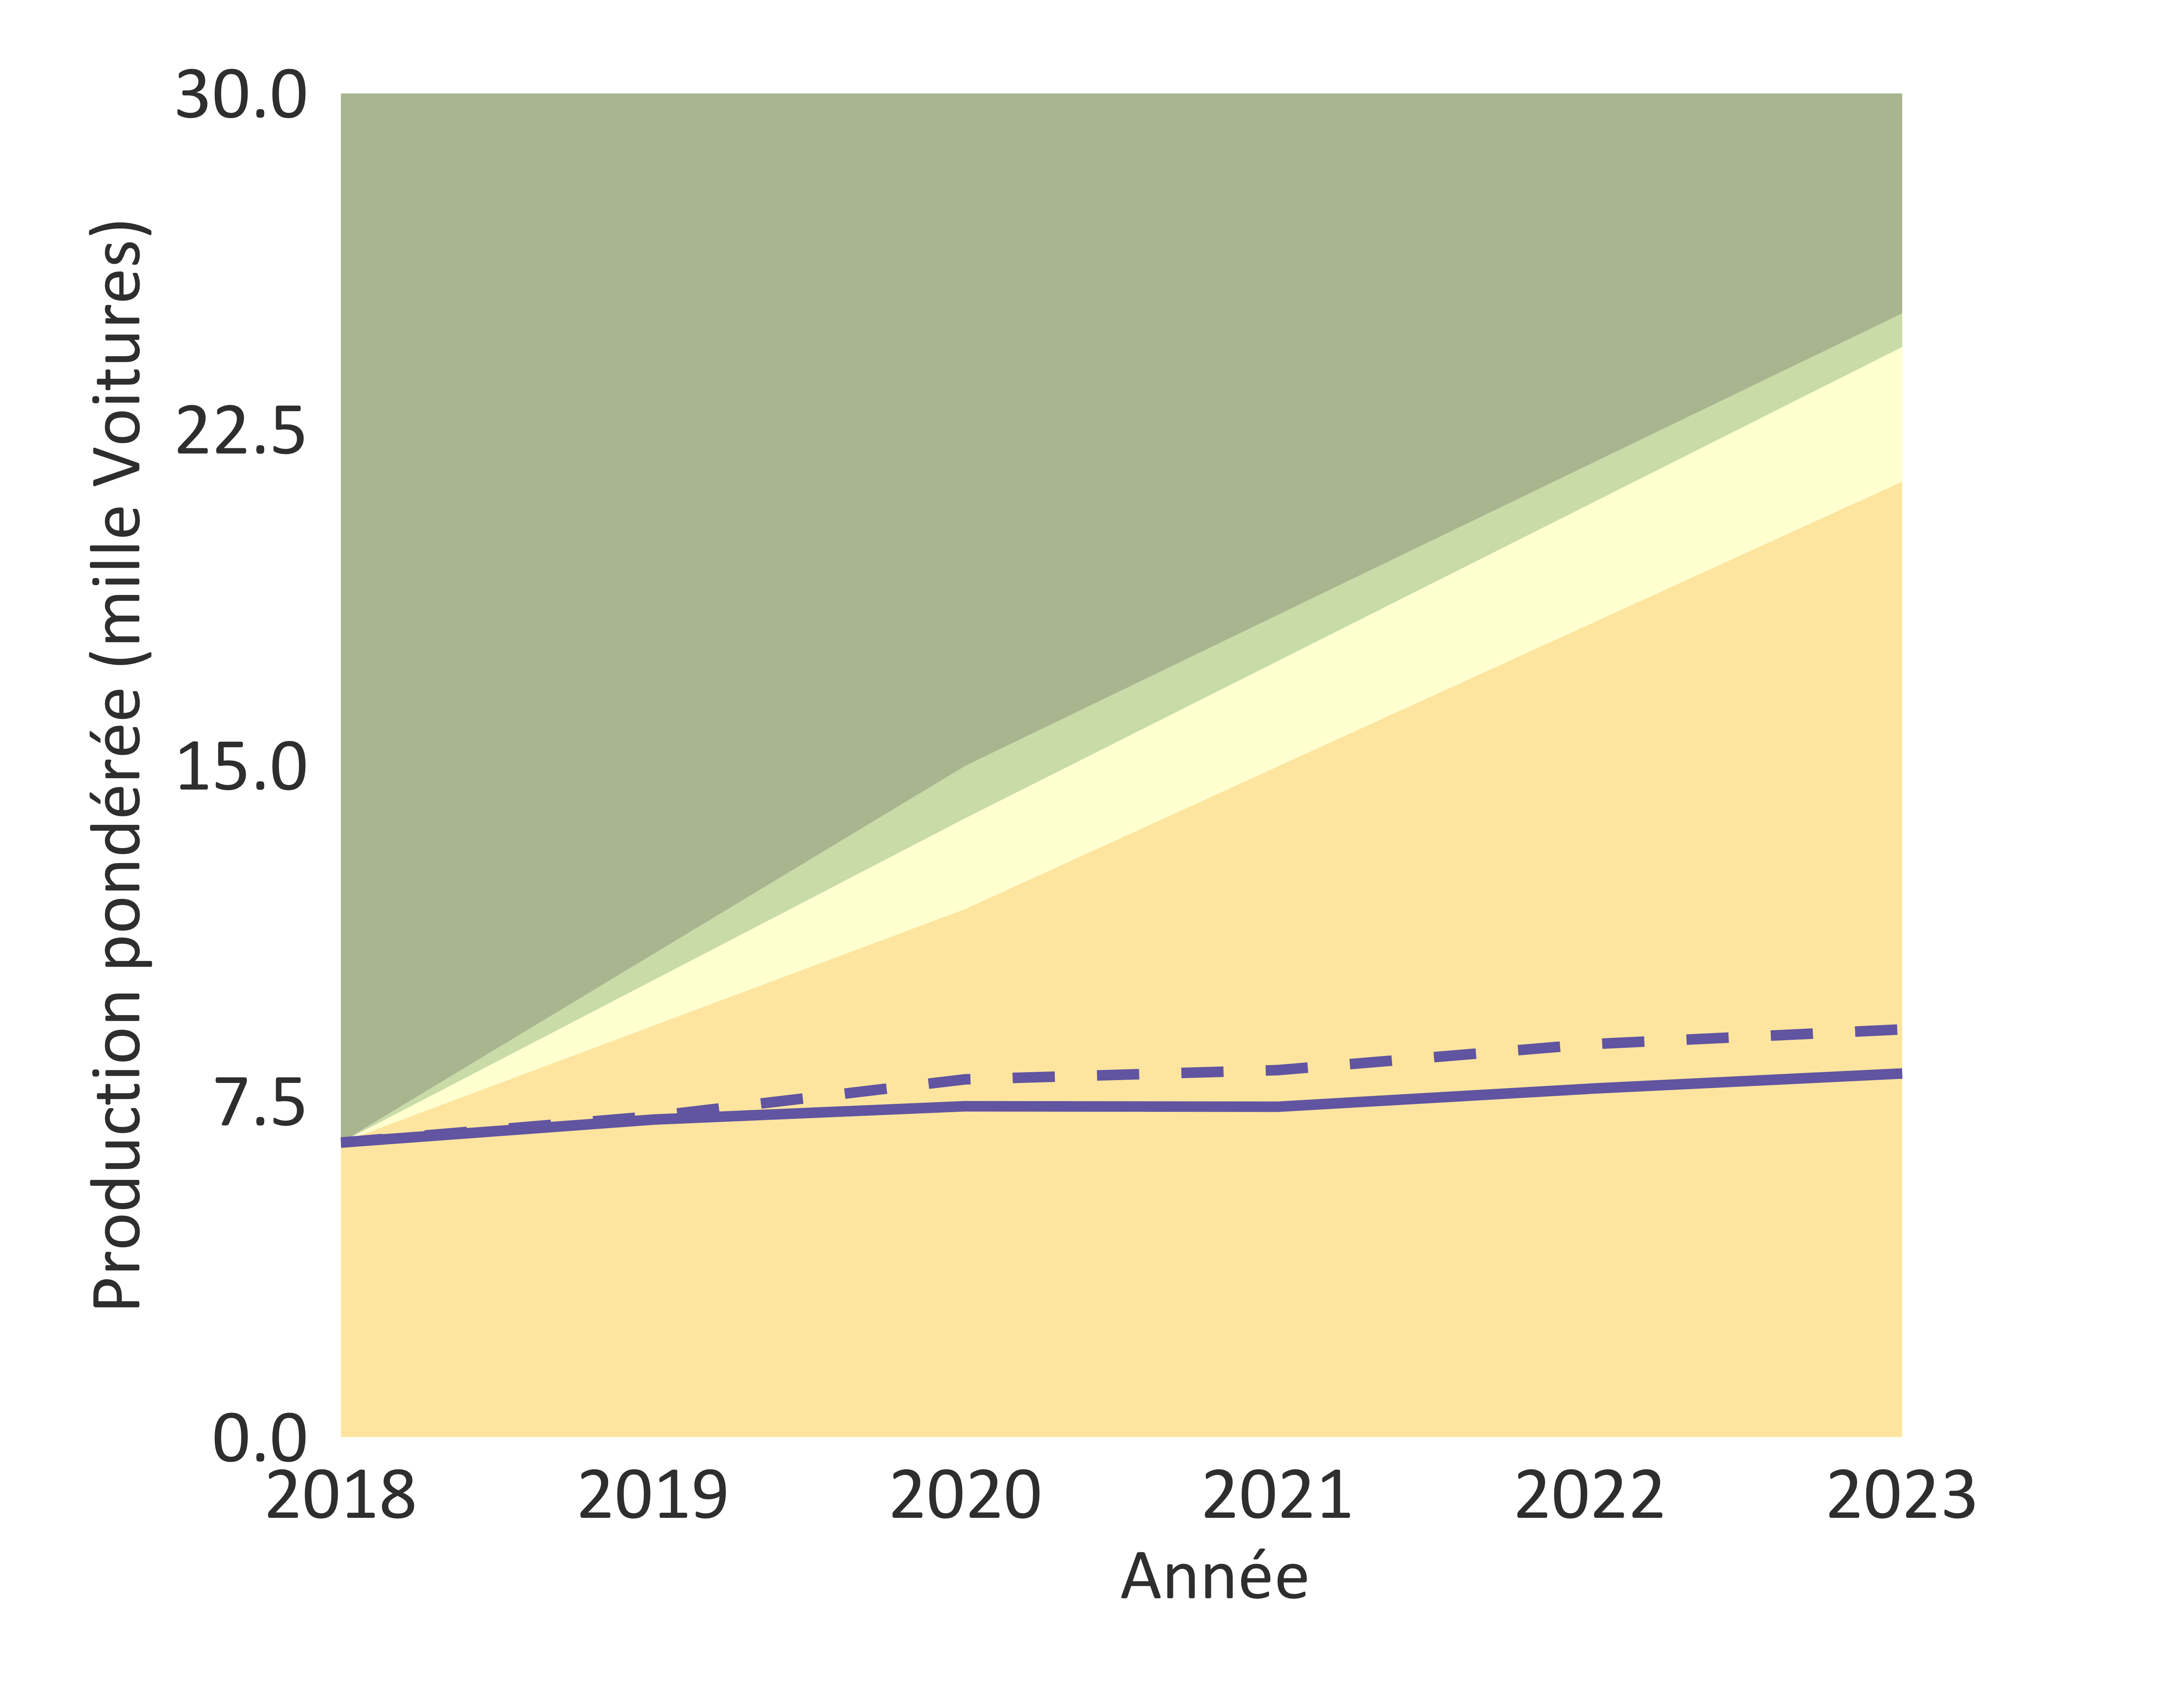
\includegraphics[trim = {0 0cm 0 0},width=1\linewidth]{ReportOutputs/Fig16}
	
	\end{minipage}		
	
	\vspace{-.6cm}
	\begin{center}
		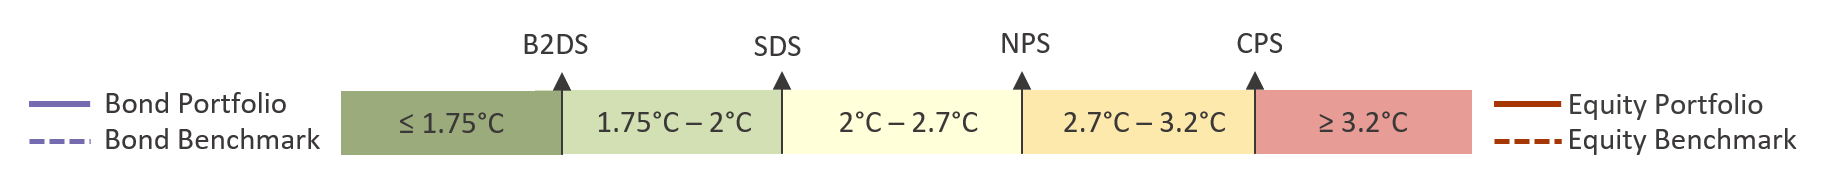
\includegraphics[trim = {0 0cm 0 0},width=.9\linewidth]{ReportGraphics/246Legend.png}
	\end{center}
	

	%\PageFooterThird
\PageFooter{3 - TRAJECTORY OF THE PORTFOLIO}
	
	\newpage 
	%AutoSector_CBE 
	%AutoSector_EQS	
	\section*{} % TRAJECTORY - EQUITY - FOSSIL FUELS AND AUTOMOTIVE 
		\HeaderDouble{5 YEAR TREND - EQUITY}{AUTOMOTIVE}	
	
	\begin{multicols}{2}
		\textbf{The alignment graphs below show the alignment of automobile technologies in the equity portfolio relative to the IEA scenarios: B2DS (well below 2°C), SDS (2°C), NPS (4°C), CPS (6°C) and the global equity market. } 
		For each technology, the value plotted for the portfolio (solid line) is the planned evolution of automobile production allocated to the equity portfolio over the next 5 years.  The lines separating the color-coded background areas plot the portfolio's target production for each technology under the IEA scenarios. The dotted line shows planned production in the specific technology for the listed equity market, scaled to the same starting point as the portfolio.                    
		
	\end{multicols}		
	
	
	\begin{minipage}[t]{.49\linewidth}
		\textbf{Trajectory of ICE Vehicle Production}
		
		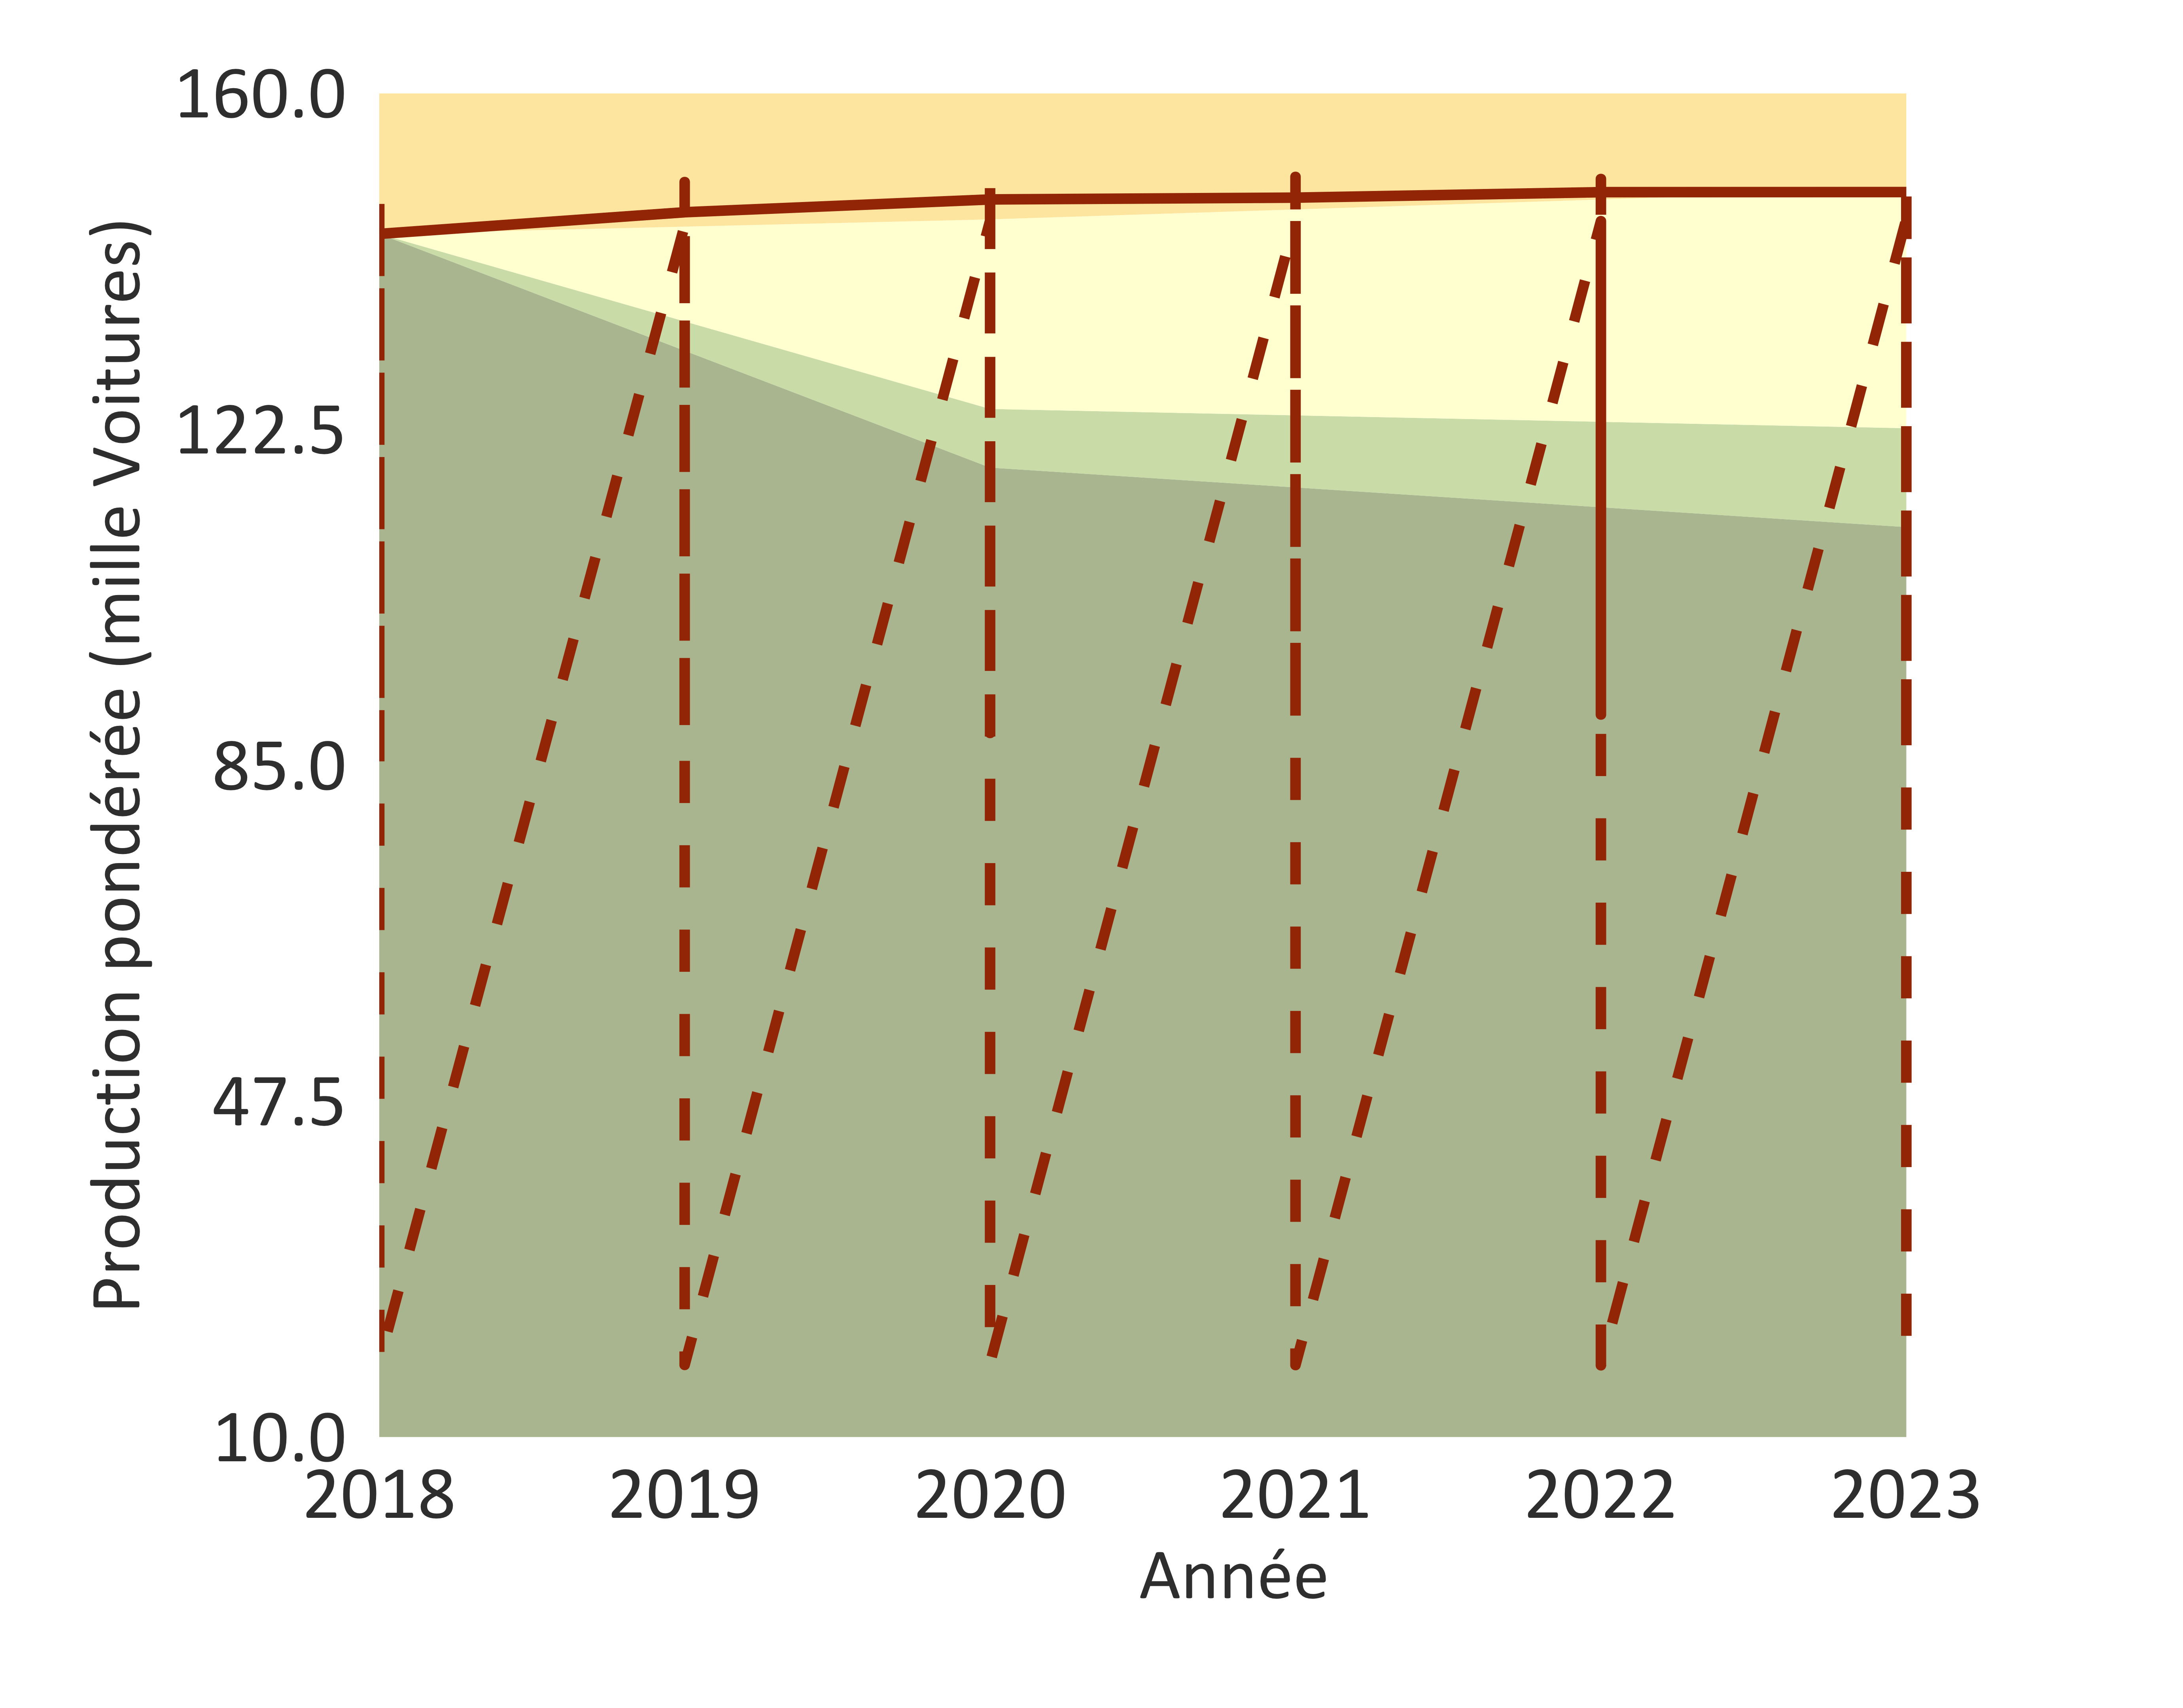
\includegraphics[trim = {0 0cm 0 0},width=1\linewidth]{ReportOutputs/Fig24}
		
	\end{minipage}	
	\hspace{.02\linewidth}
	\begin{minipage}[t]{.49\textwidth}
		\textbf{Trajectory of Electric Vehicle Production}
		
		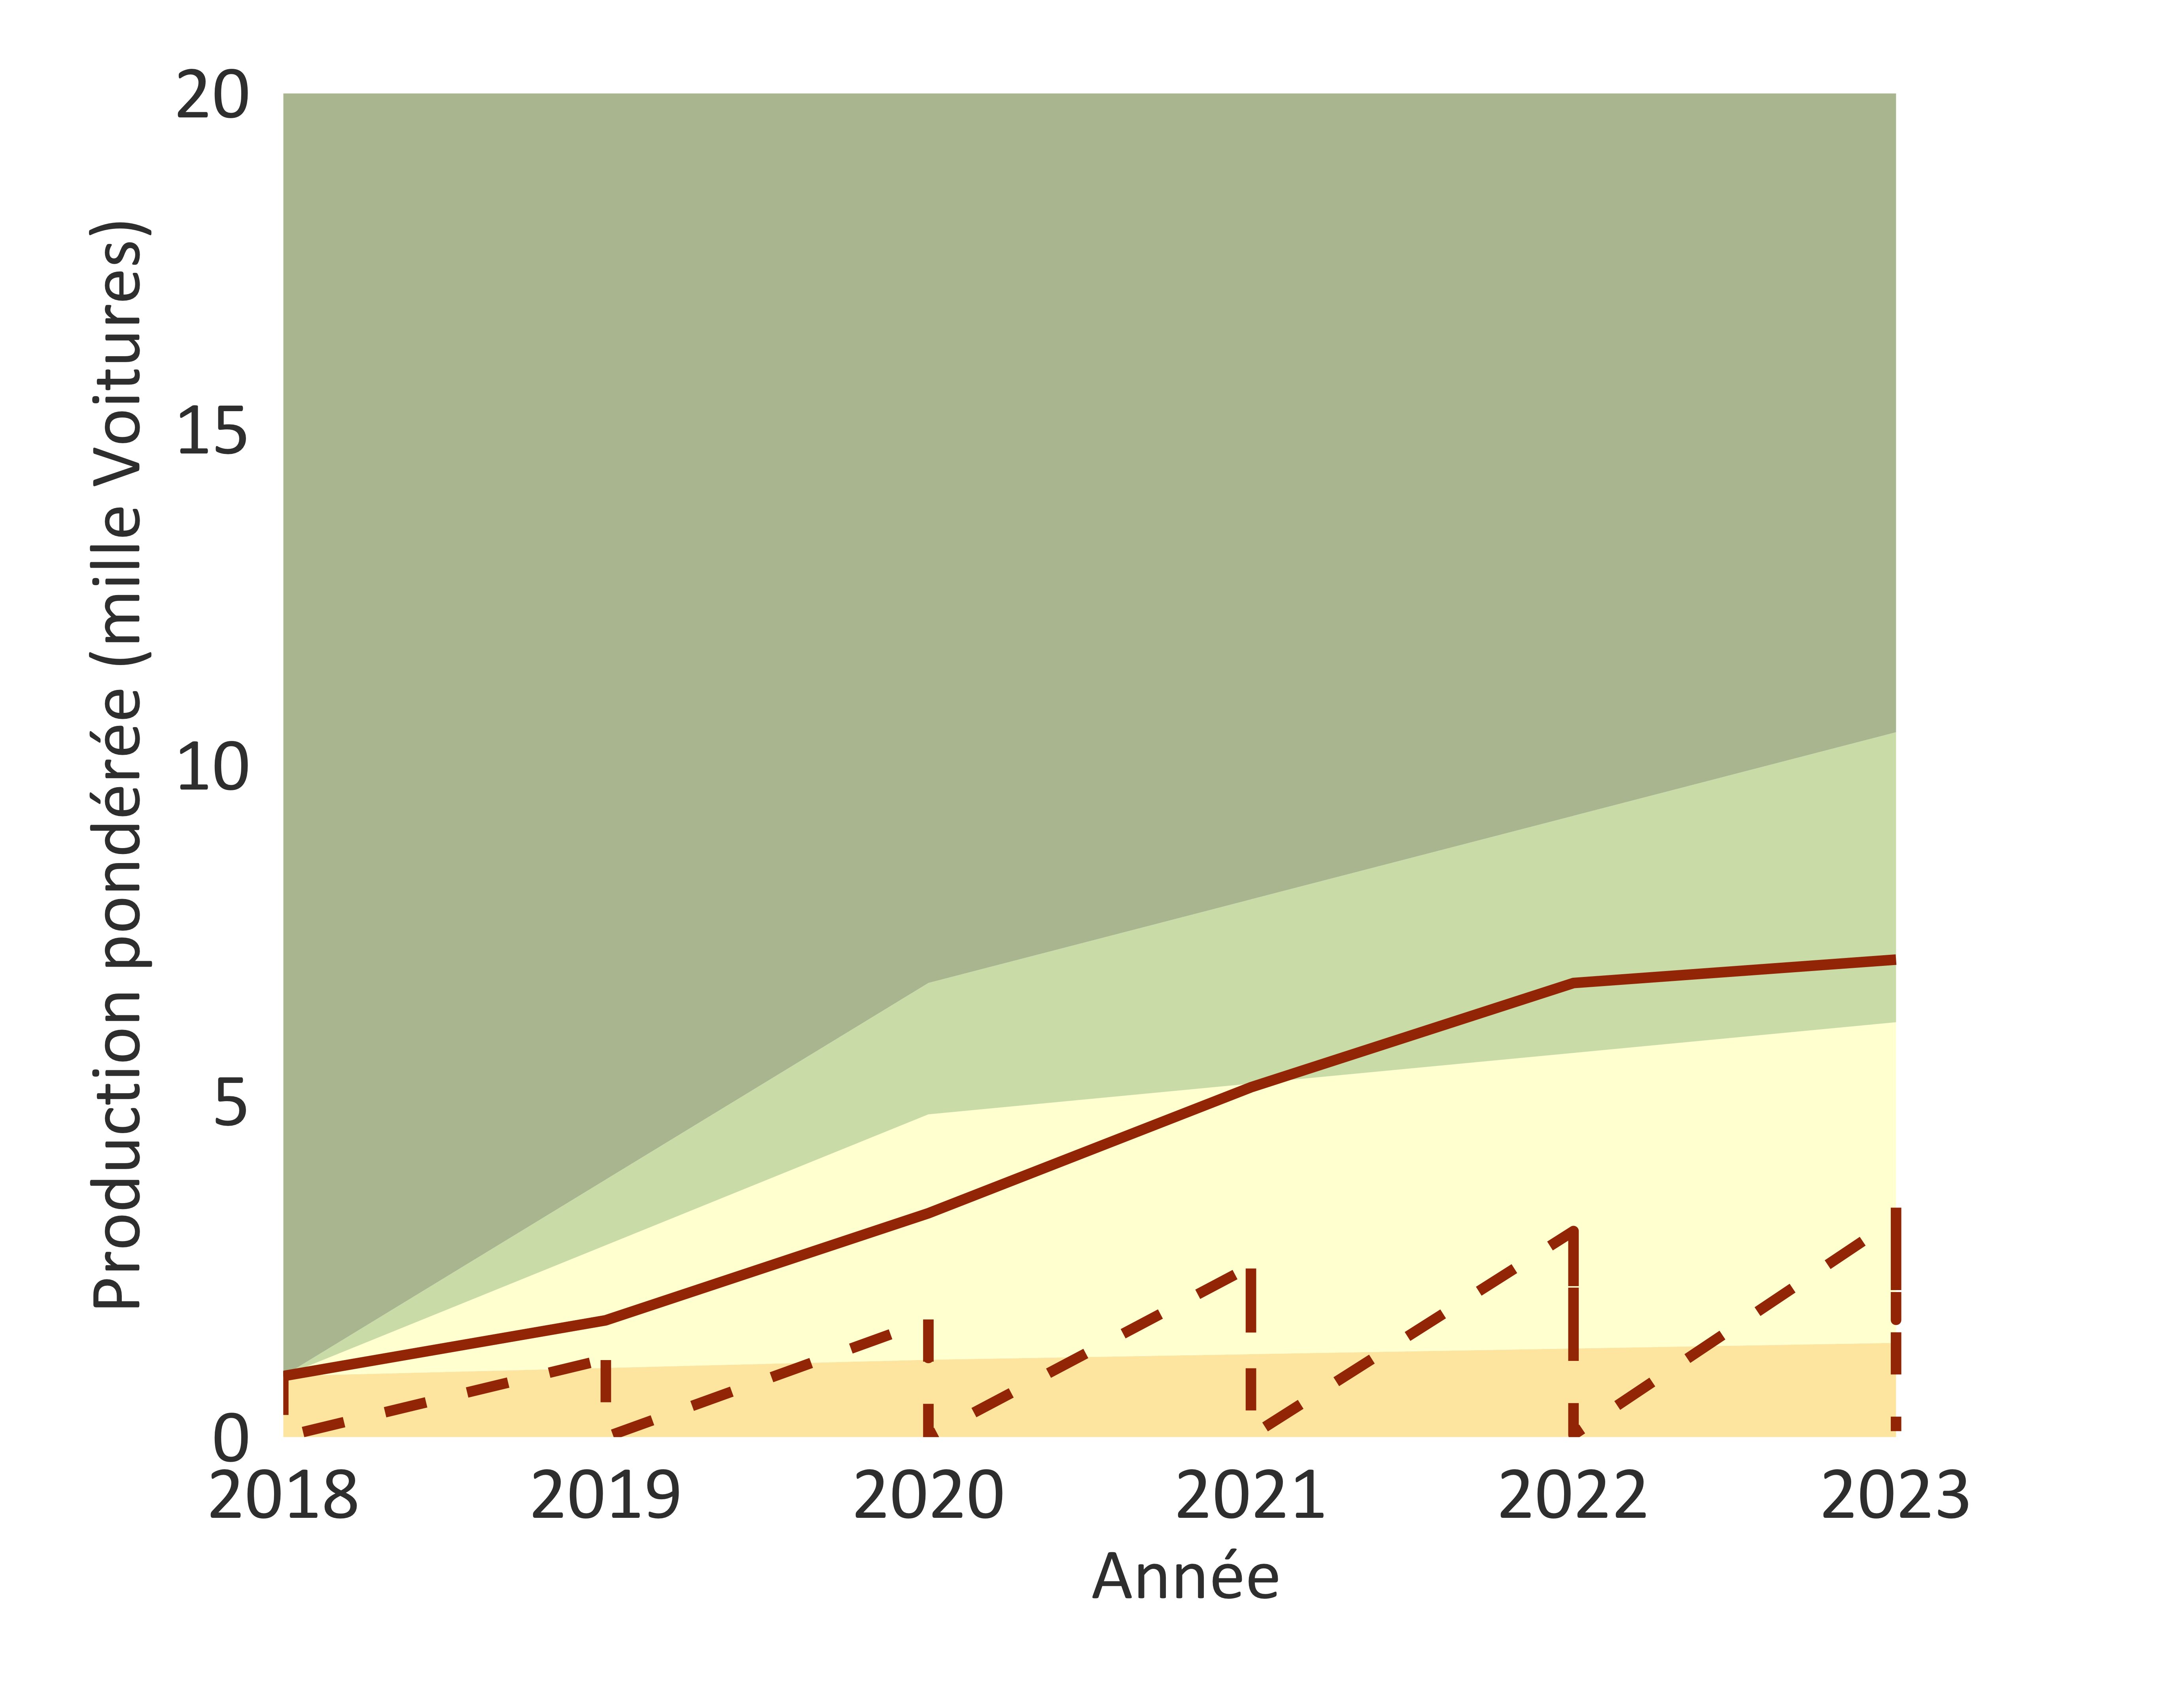
\includegraphics[trim = {0 0cm 0 0},width=1\linewidth]{ReportOutputs/Fig25}
		
	\end{minipage}	
	
	\begin{minipage}[t]{.49\textwidth}
		\textbf{Trajectory of Hybrid Vehicle Production}
		
		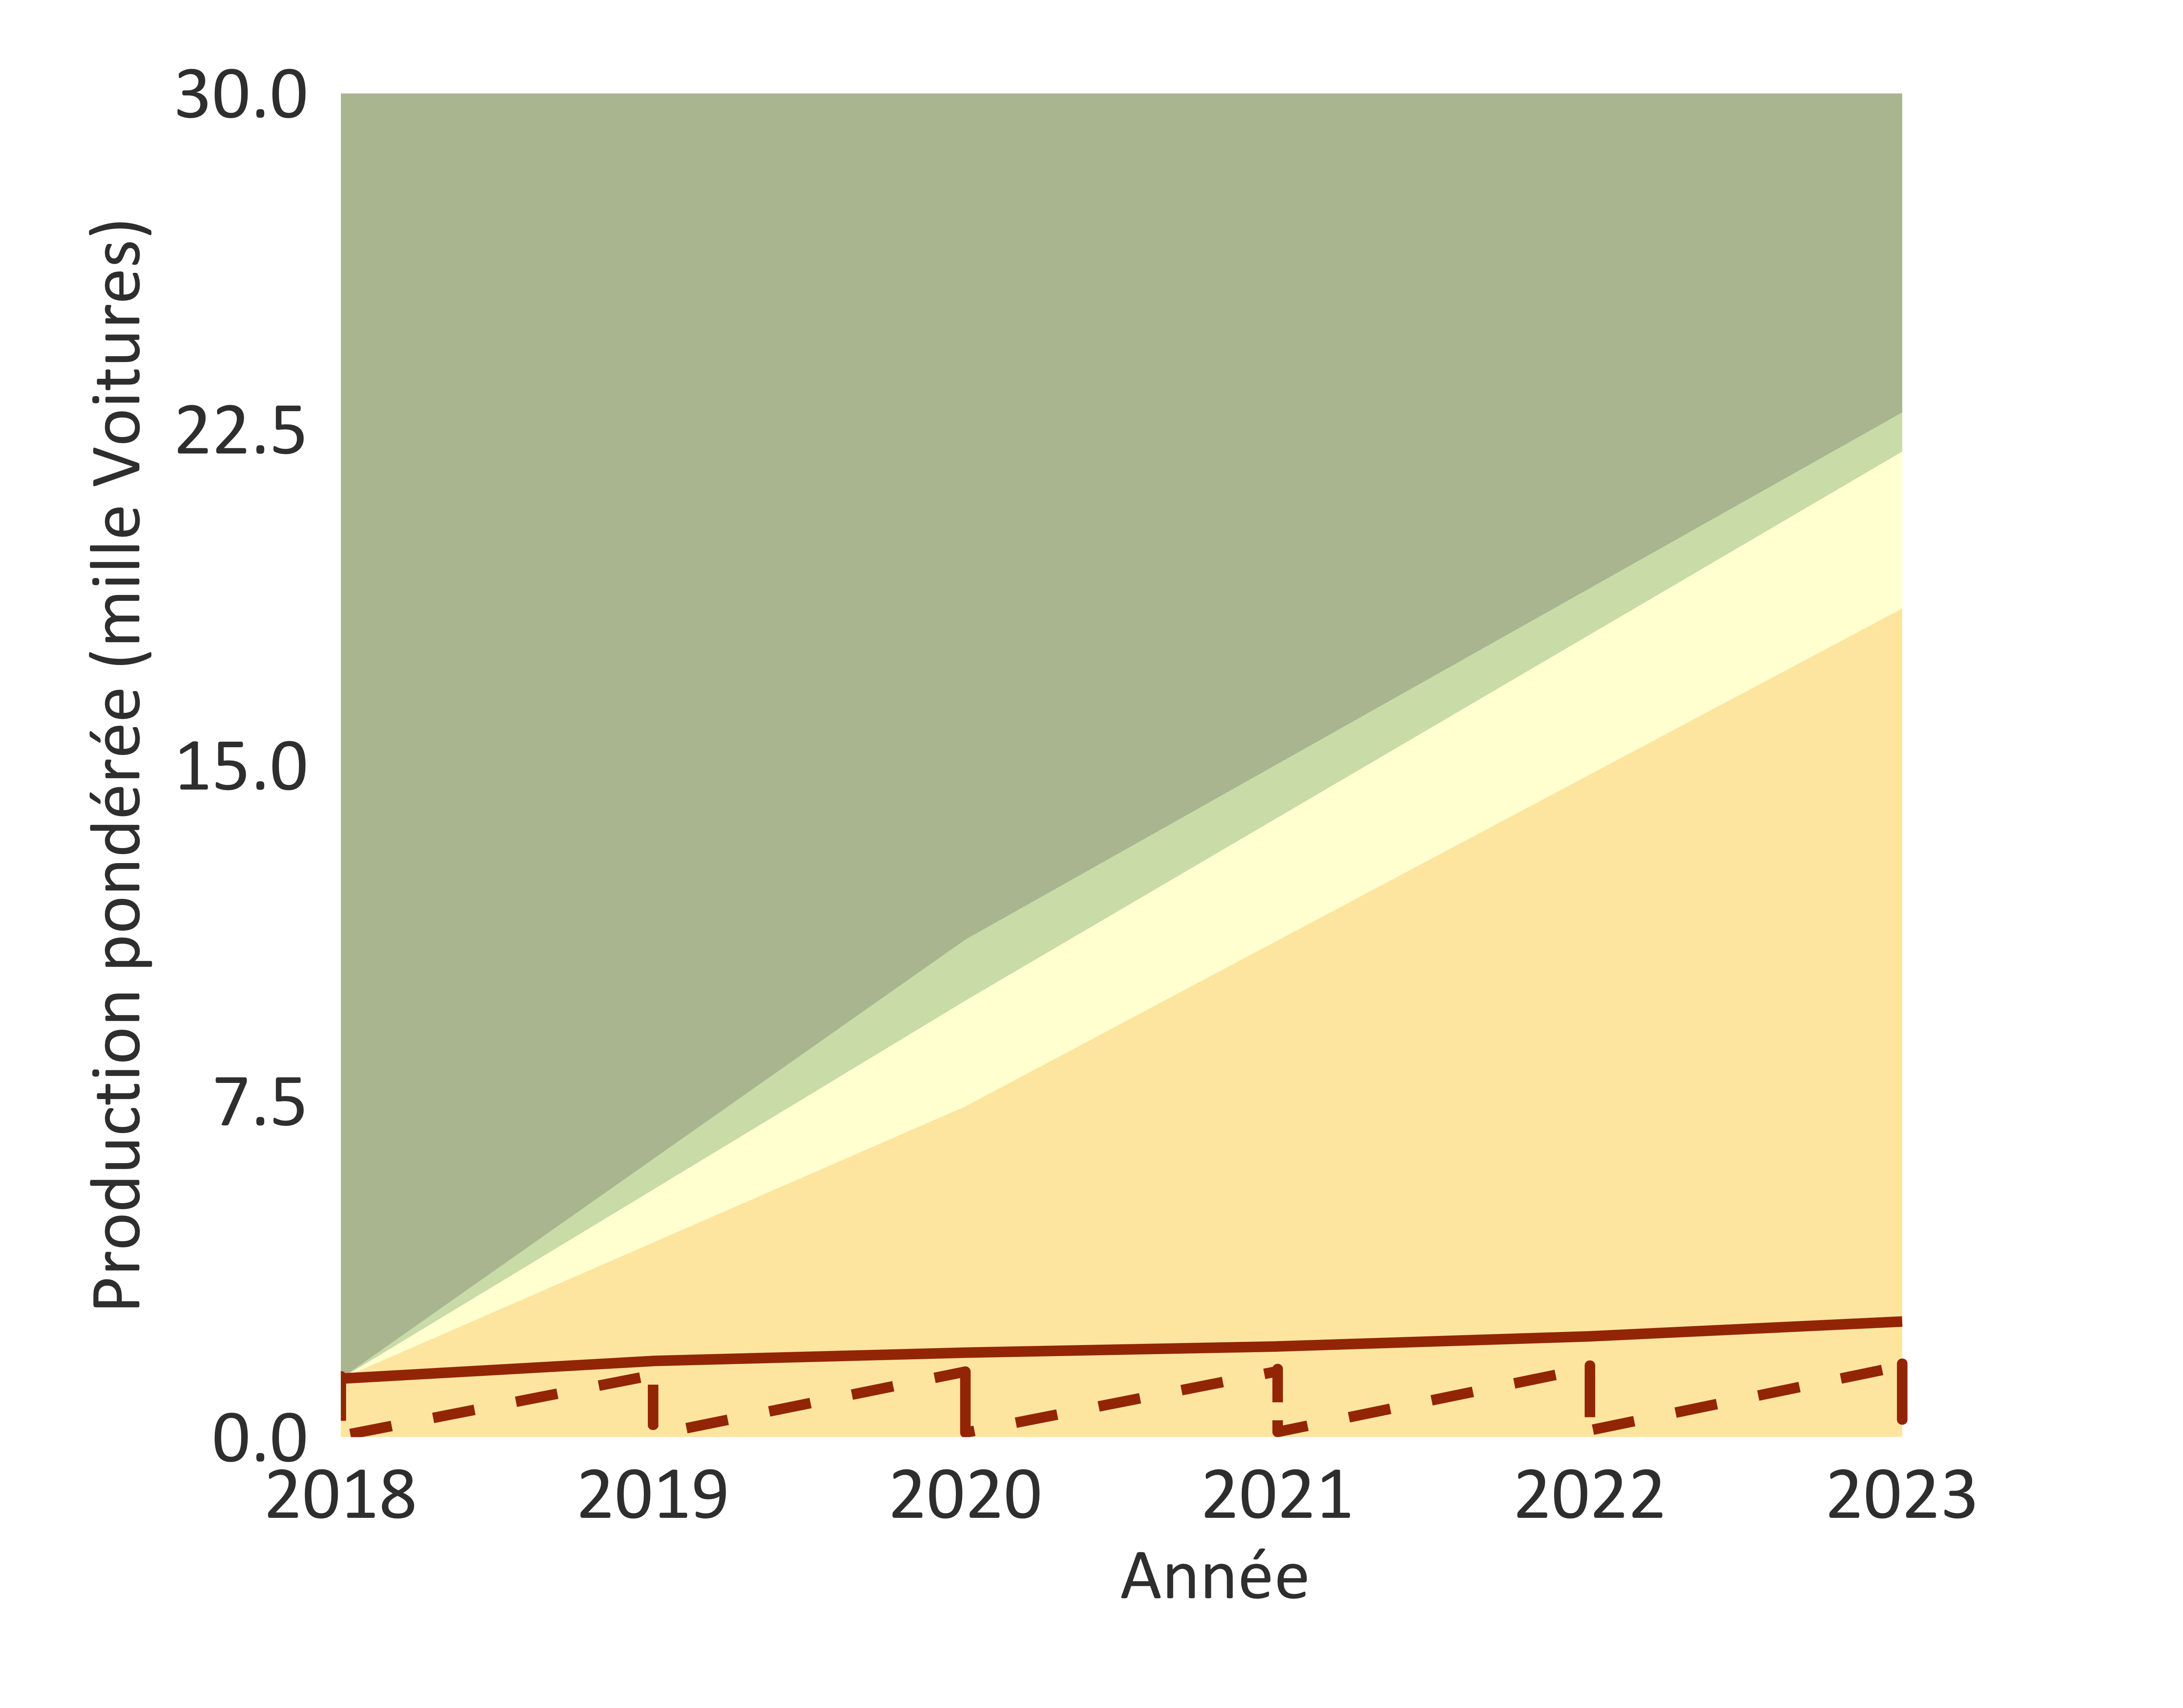
\includegraphics[trim = {0 0cm 0 0},width=1\linewidth]{ReportOutputs/Fig26}
		
	\end{minipage}		
	
	\vspace{-.6cm}
	\begin{center}
		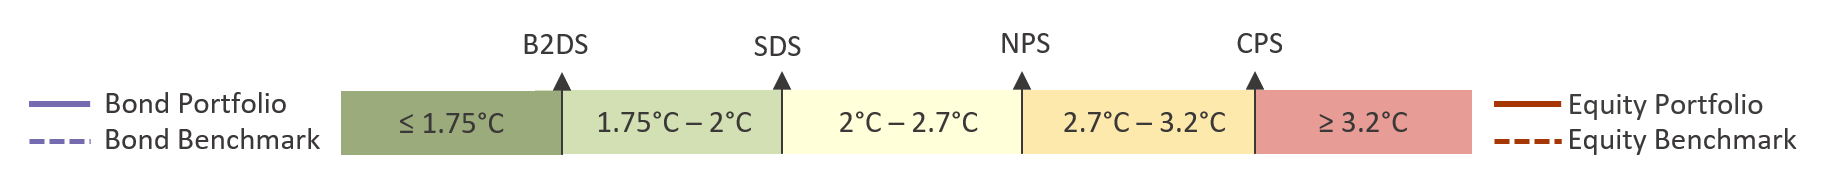
\includegraphics[trim = {0 0cm 0 0},width=.9\linewidth]{ReportGraphics/246Legend.png}
	\end{center}
	
	
	%\PageFooterThird
\PageFooter{3 - TRAJECTORY OF THE PORTFOLIO}
	
	\newpage 
	%AutoSector_EQE
	%AutoSector_ALLE
	%OtherSectorsS
	\section*{} % OTHER SECTORS 
	\HeaderSingle{EMISSION INTENSITY ANALYSIS}
	
	\begin{multicols}{2}
		There are a number of sectors for which no substitutable lower carbon technologies exist at scale on the market or there is insufficient asset level or scenario data. This is relevant to the steel, cement, shipping and air transport sectors. For these sectors, an analysis of the required changes in emissions intensity is conducted. 
	
		For these sectors, decarbonisation efforts are confined to increasing efficiency in production and use, as well as investment in research and development in the next 5-10 years, in order to bring CO\textsubscript{2}-neutral alternatives to market maturity in the medium term. As a result, both the scenarios and the data are relatively imprecise.
	
		The figures presented below are based on external CO\textsubscript{2} intensity estimates, based on a publicly available emissions estimation model developed by 2Dii together with the consulting company Ernst \& Young. For shipping, an external CO\textsubscript{2} rating model developed by Rightship and the Carbon War Room has been used. A rating of A is indicative of best in class ship efficiency and G worst in class. Since this model is estimated externally and top-down, it is associated with some uncertainties. The results should therefore be considered as estimates, in contrast to the scenario analysis of the energy, electricity and automotive sectors. More information can be found in Section 6. 
	\end{multicols}
	
	\begin{multicols}{2}
		
		\textbf{Cement}
		
		\textbf{Steel}
		
	\end{multicols}
	
	\setlength\multicolsep{0pt}
	\vspace{0cm}
	
	\begin{multicols}{2}
		
		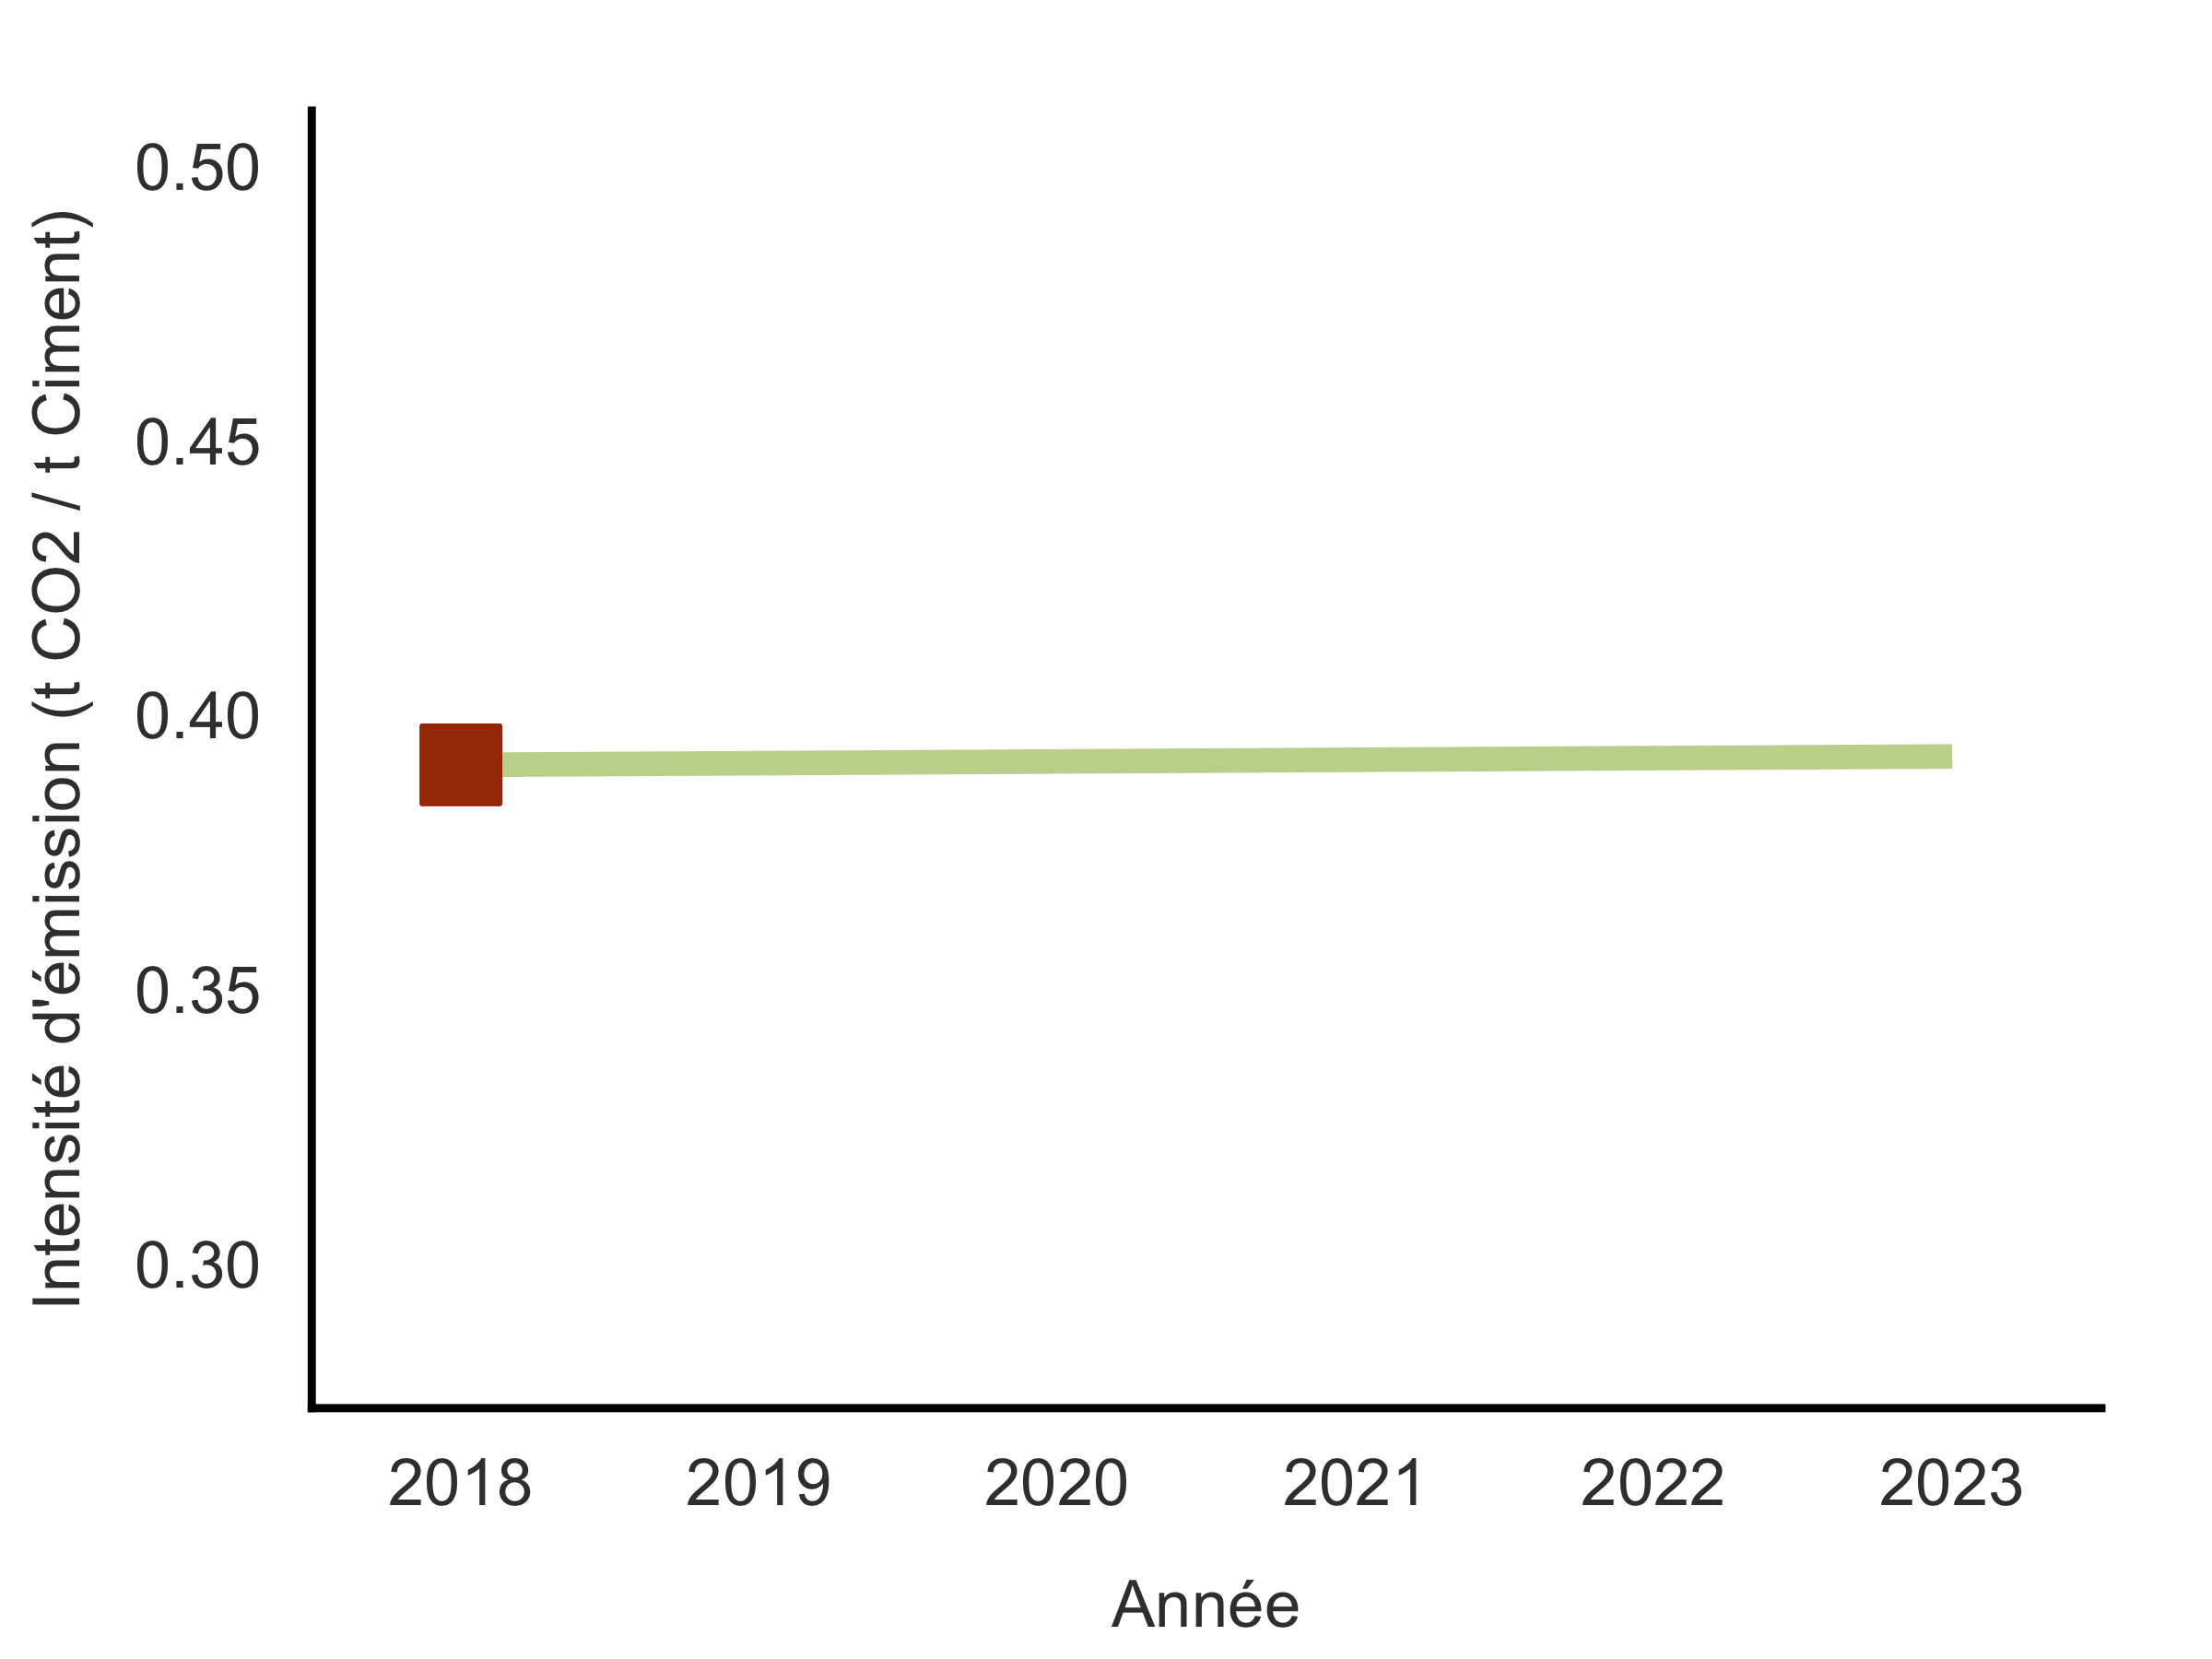
\includegraphics[width=.9\linewidth]{ReportOutputs/Fig30} \vfill\null \columnbreak
		
		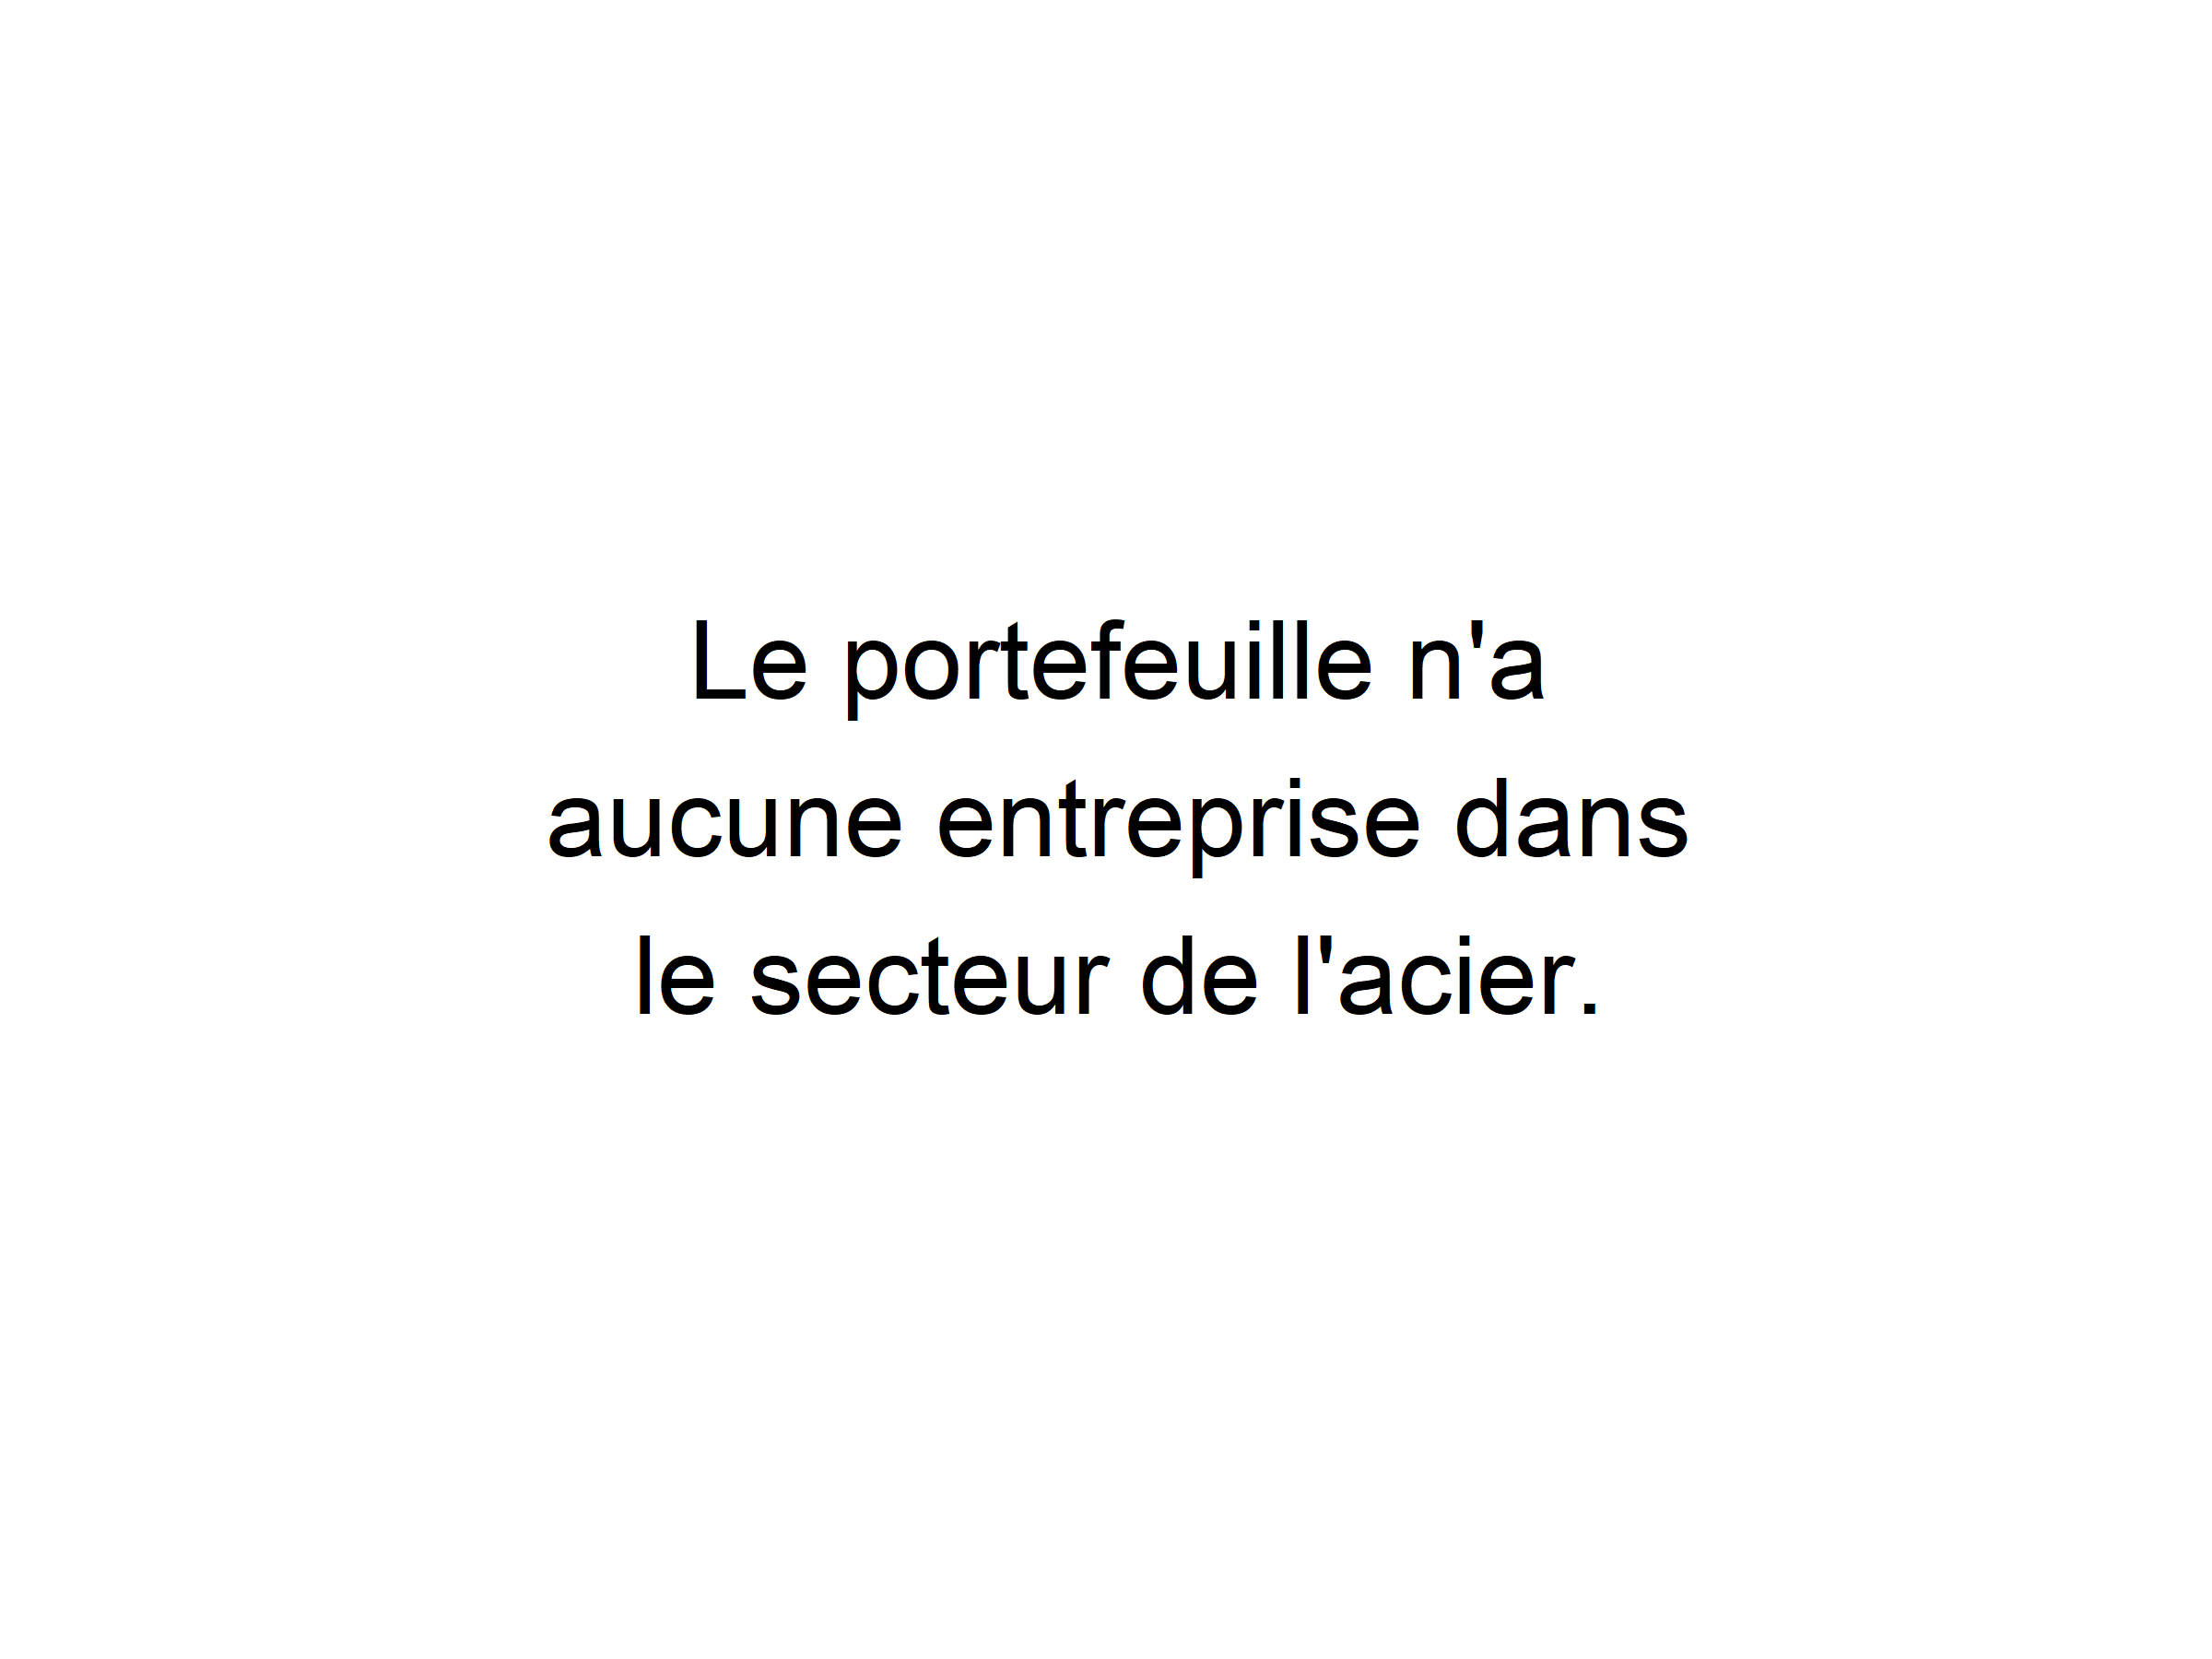
\includegraphics[width=.9\linewidth]{ReportOutputs/Fig31}
		
	\end{multicols}
	
	\begin{multicols}{2}
		
		\textbf{Aviation}
		
		\textbf{Shipping}
		
	\end{multicols}
	
	\vspace{0cm}
	
	\begin{multicols}{2}
		
		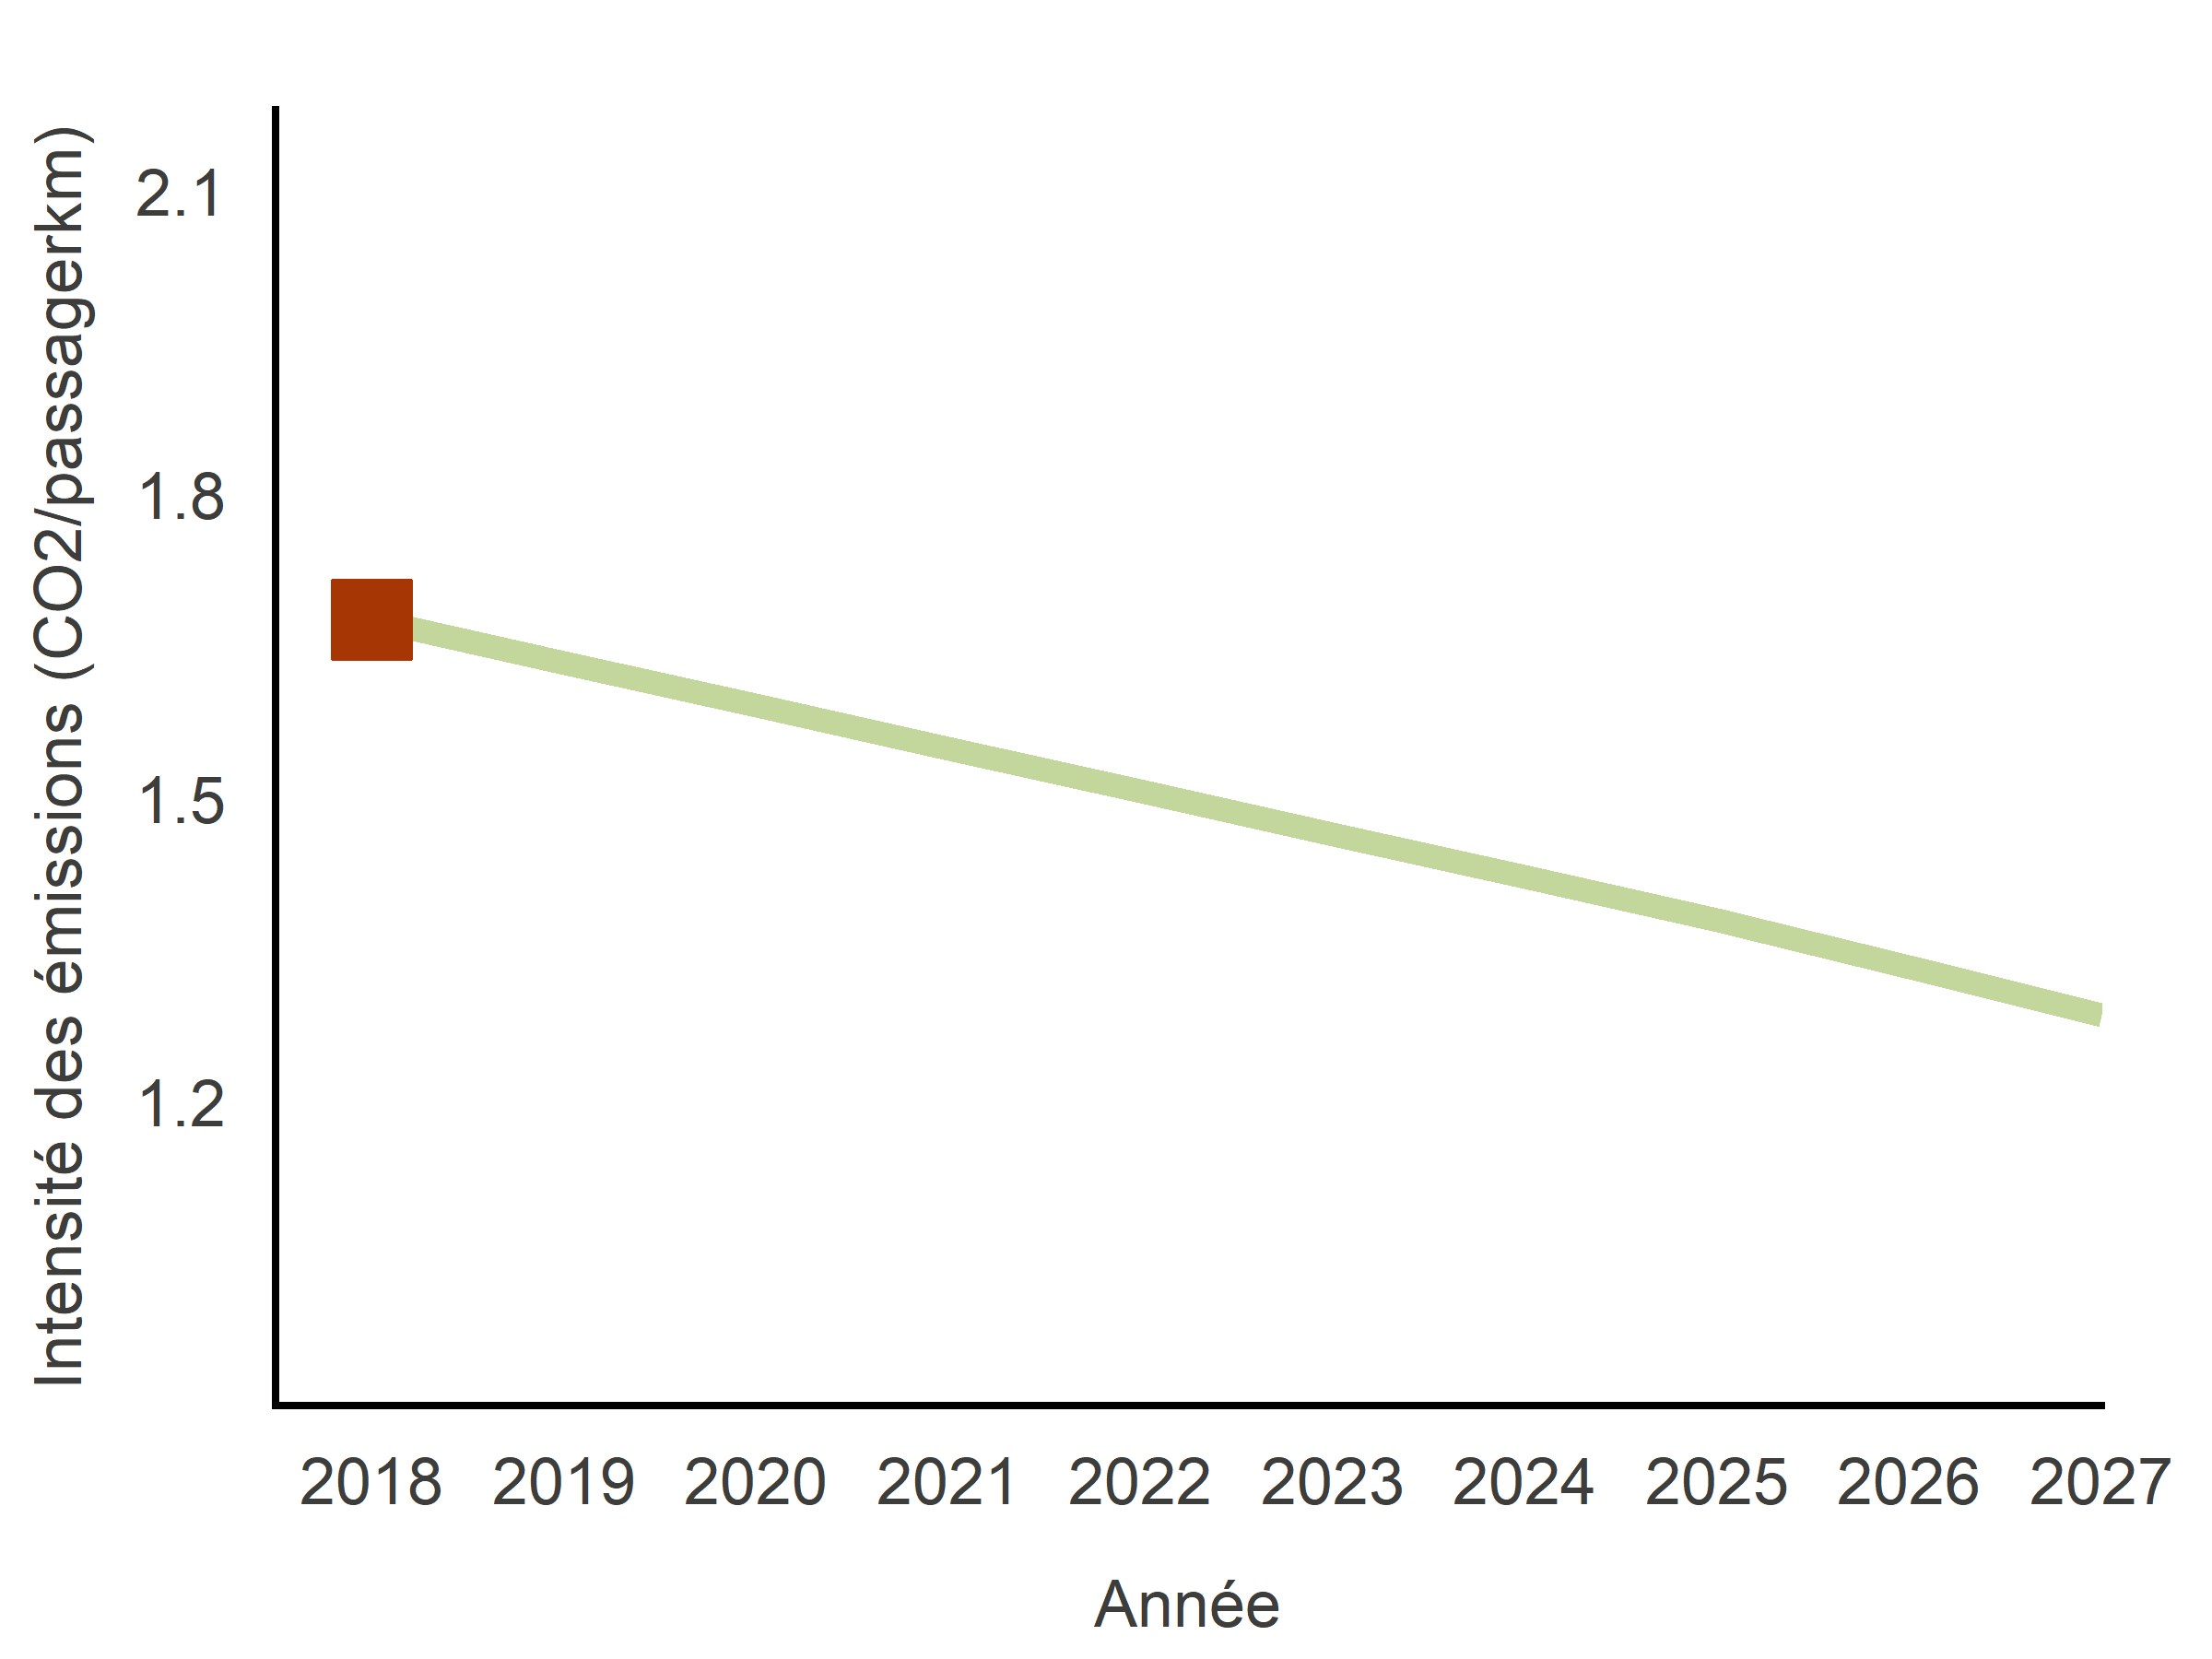
\includegraphics[trim = {0 0 0 0pt}, width=.9\linewidth]{ReportOutputs/Fig32}  \vfill\null \columnbreak
		
		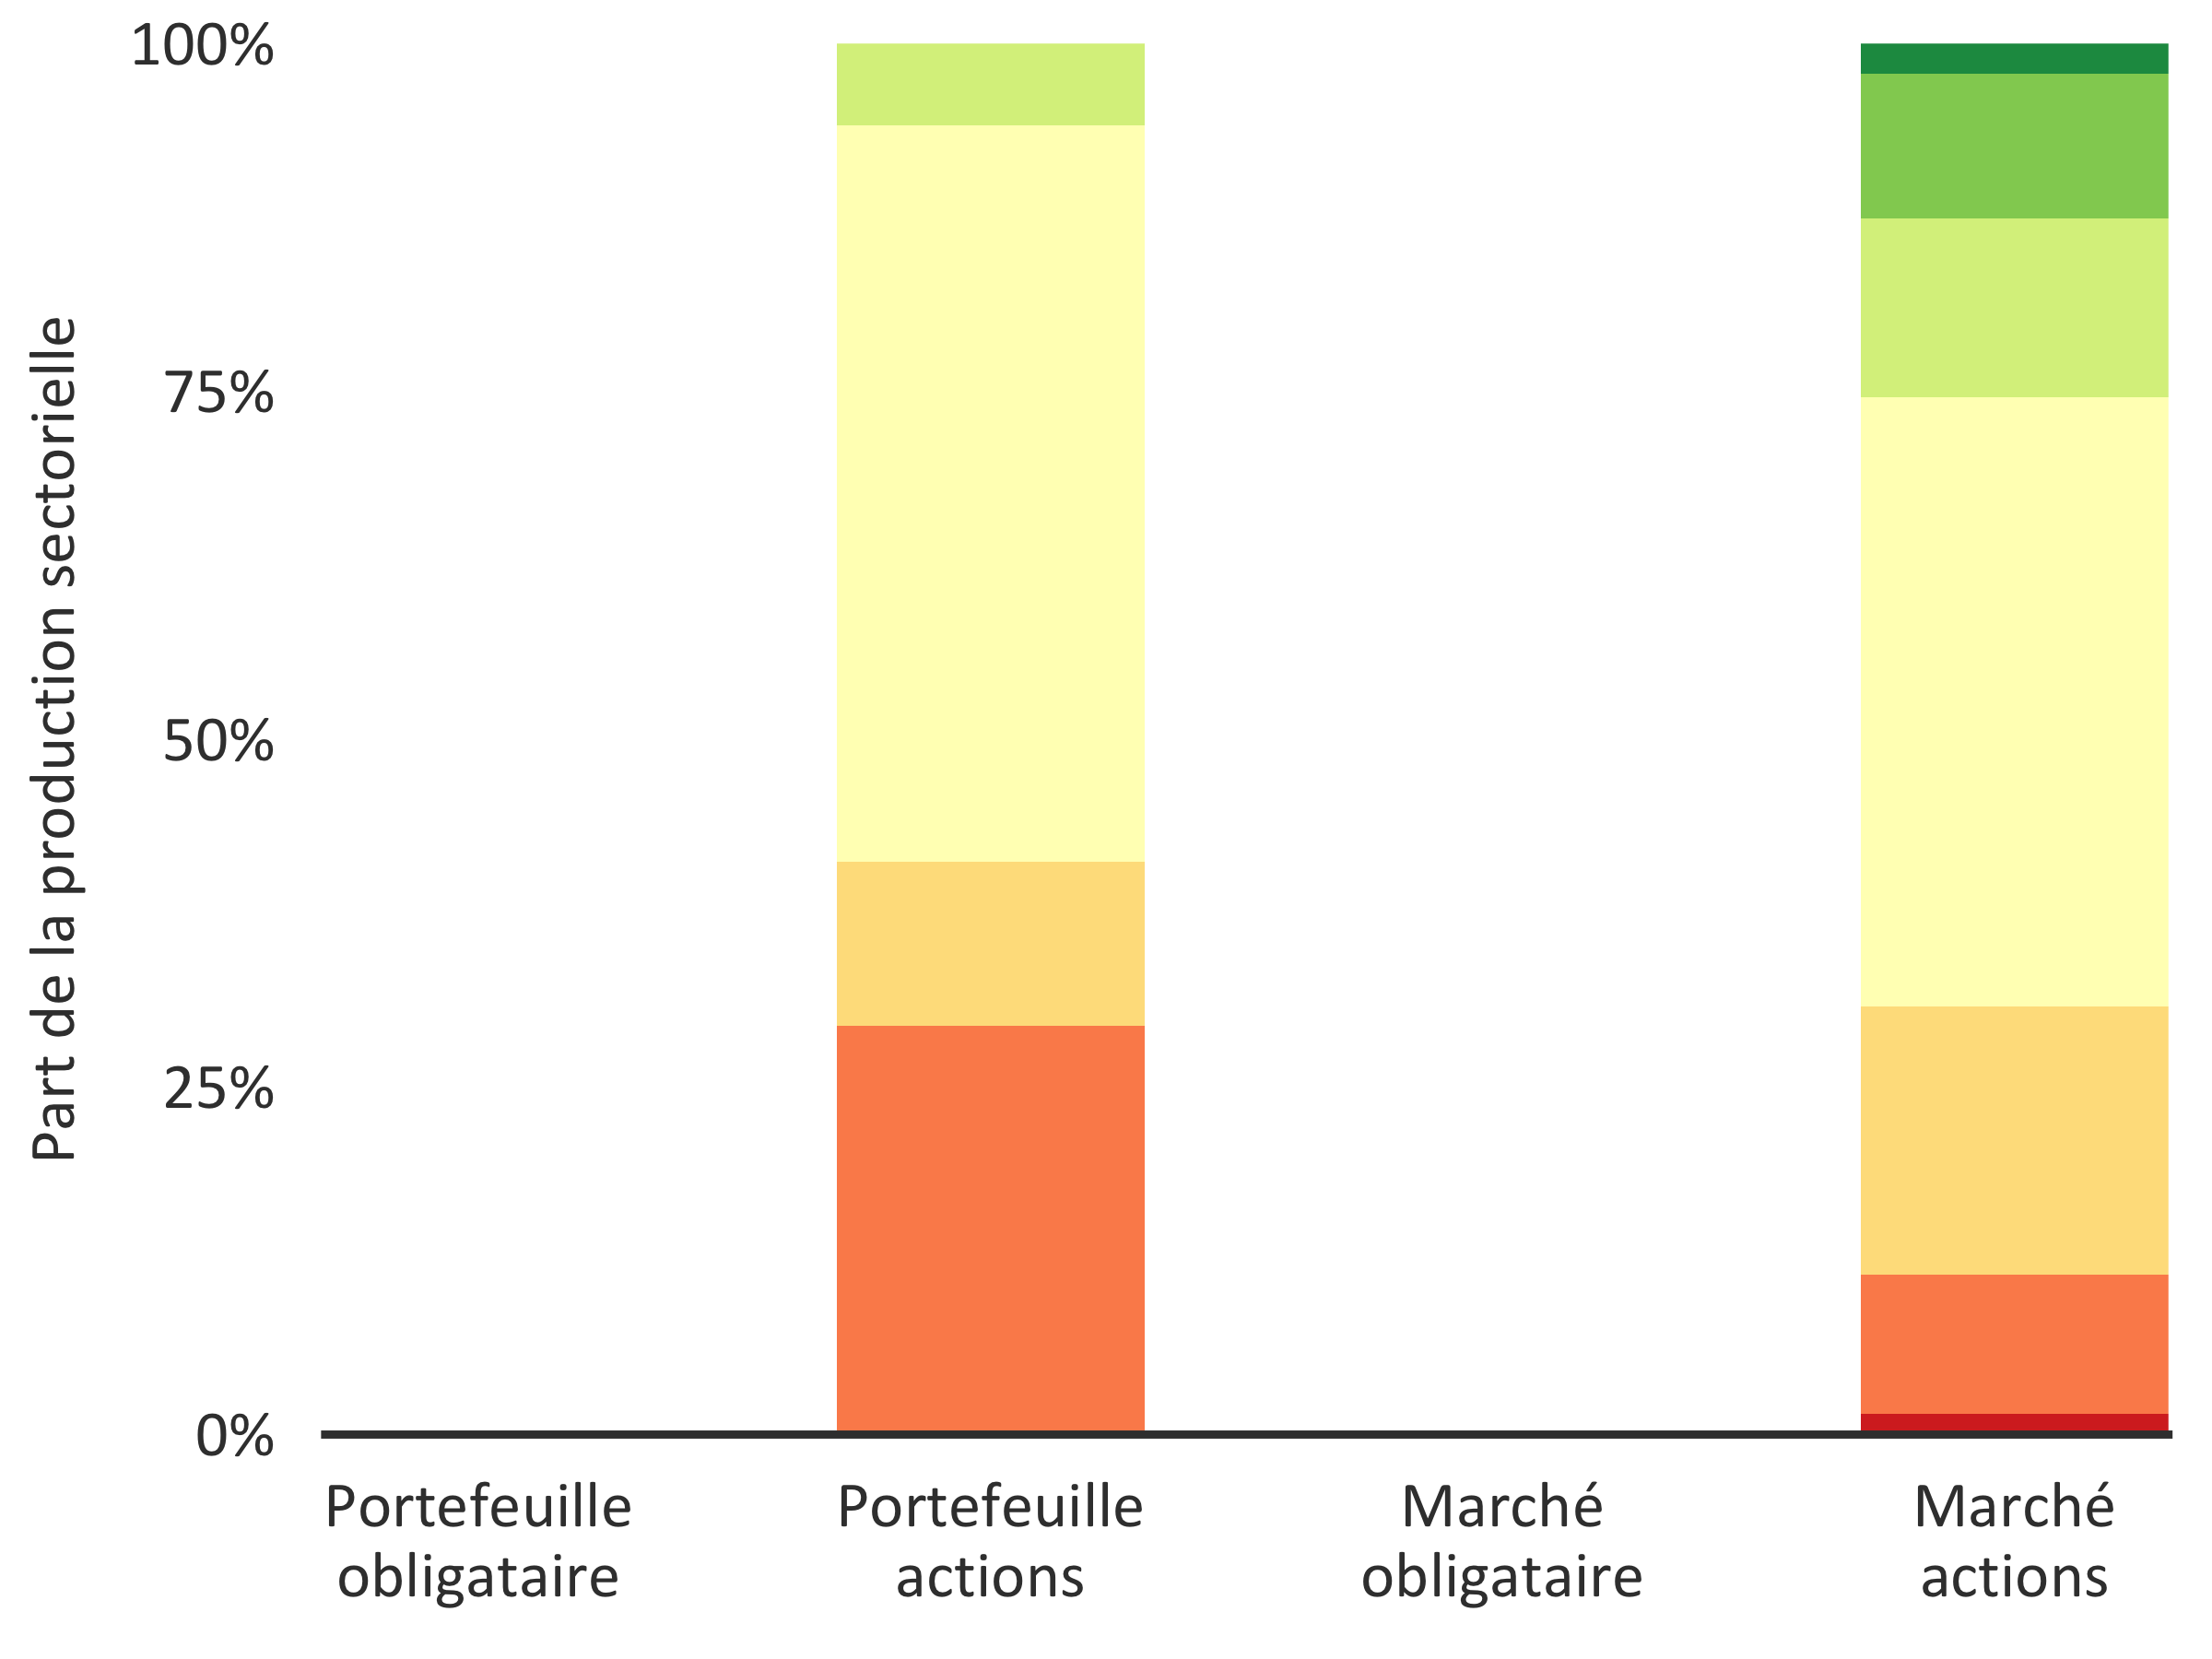
\includegraphics[width=1\linewidth]{ReportOutputs/Fig33}
		
	\end{multicols}
	
	\vspace{0pt}
	\setlength\multicolsep{0pt}
	
	\begin{multicols}{2}
		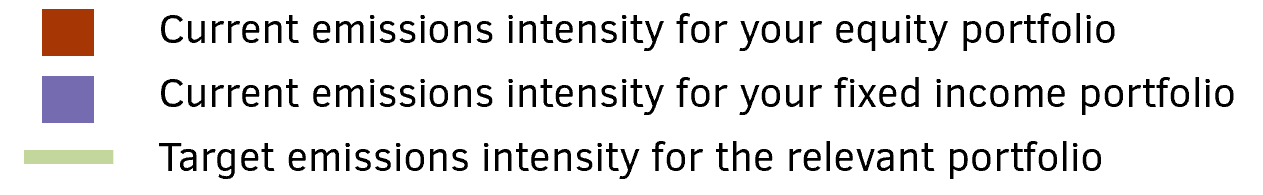
\includegraphics[width=1\linewidth]{ReportGraphics/OtherSectorLegend}
		
		
		%NoShippingS
		\begin{center}
			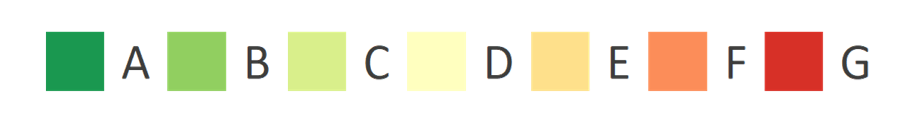
\includegraphics[width=0.6\linewidth]{ReportGraphics/ShippingLegend}
		\end{center}	
		%NoShippingE		
		
	\end{multicols}
	
	\textit{\small Source: 2Dii based on EY 2016, PlantFacts, FlightAscend, Rightship, Carbon War Room, IEA 2017 and SDA 2015}
	
	\setlength\multicolsep{12pt}
	
	%\PageFooterThird 
\PageFooter{3 - TRAJECTORY OF THE PORTFOLIO}
	
	\newpage 
	% OtherSectorsE
	\section*{} % 4th SECTION 
	\SectionHeadingDouble{SECTION 4:}{THE EXPOSURE OF THE PORTFOLIO}{TO THE ScenarioValue IN Startyear+5}
	
	
	\newpage
	\section*{} % FUTURE TECHNOLOGY SHARE
	\HeaderSingle{FUTURE TECHNOLOGY SHARE}
	
	\begin{multicols}{2}
		\textbf{The figure below shows the estimated exposure in Startyear+5 to high-carbon and low-carbon technologies for the fossil fuels, power, and automotive sector, in both the corporate bond and equity portfolios. }
		
		The results are a function both of the starting point of the exposure (Section 2) and the evolution of the exposure over time (Section 3) based on current revealed investment and production plans for all technologies. The results show the relative exposure of the portfolios across asset classes and technologies / fuels. The results are compared to the aligned market fuel mix under a ScenarioValue transition in Startyear+5. 
		
		As highlighted previously, the analysis does not include assumptions around changes in portfolio composition. Rather, it is limited to how the portfolio's  exposure to high-carbon and low-carbon technologies is set to change over time as a function of changes in company exposures, independent of portfolio composition changes. The results help contextualize the share of the sectoral exposure in Startyear+5 exposed to transition risks in terms of the share of activities that can be classified as either high-carbon or low-carbon. Given the marginal nature of renewable activities across oil and gas companies, this share has not been considered in the analysis, although it may over time represent a growing share. 
		
	\end{multicols}
	
	%CBSpecificS
	\textbf{Corporate Bonds}
	
	
	\begin{center}
		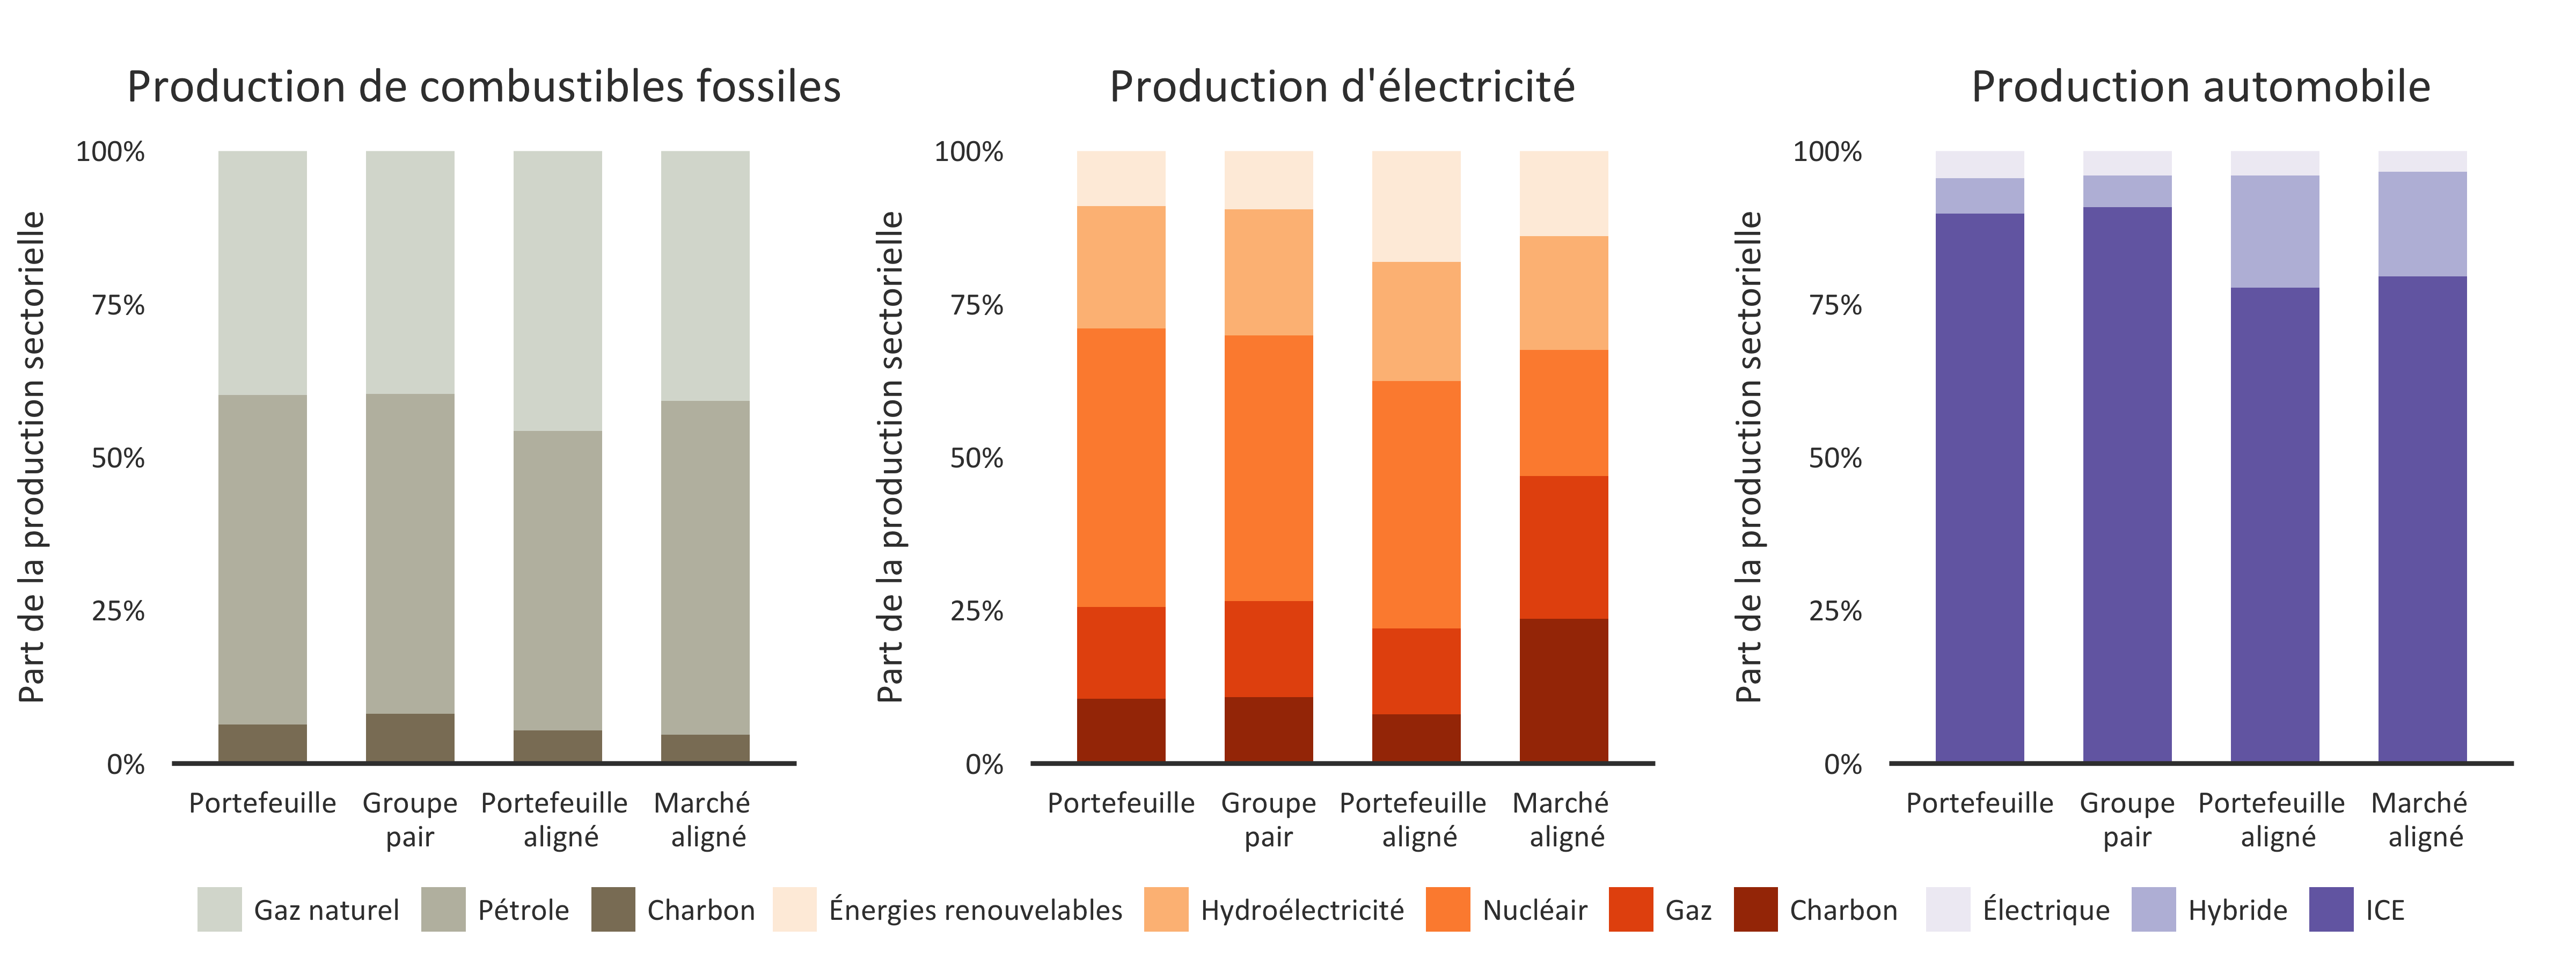
\includegraphics[trim = {0 0cm 0 0},width=1\linewidth]{ReportOutputs/Fig05}
	\end{center}
	%CBSpecificE	
	%EQSpecificS
	\textbf{Equity}
	
	
	\begin{center}
		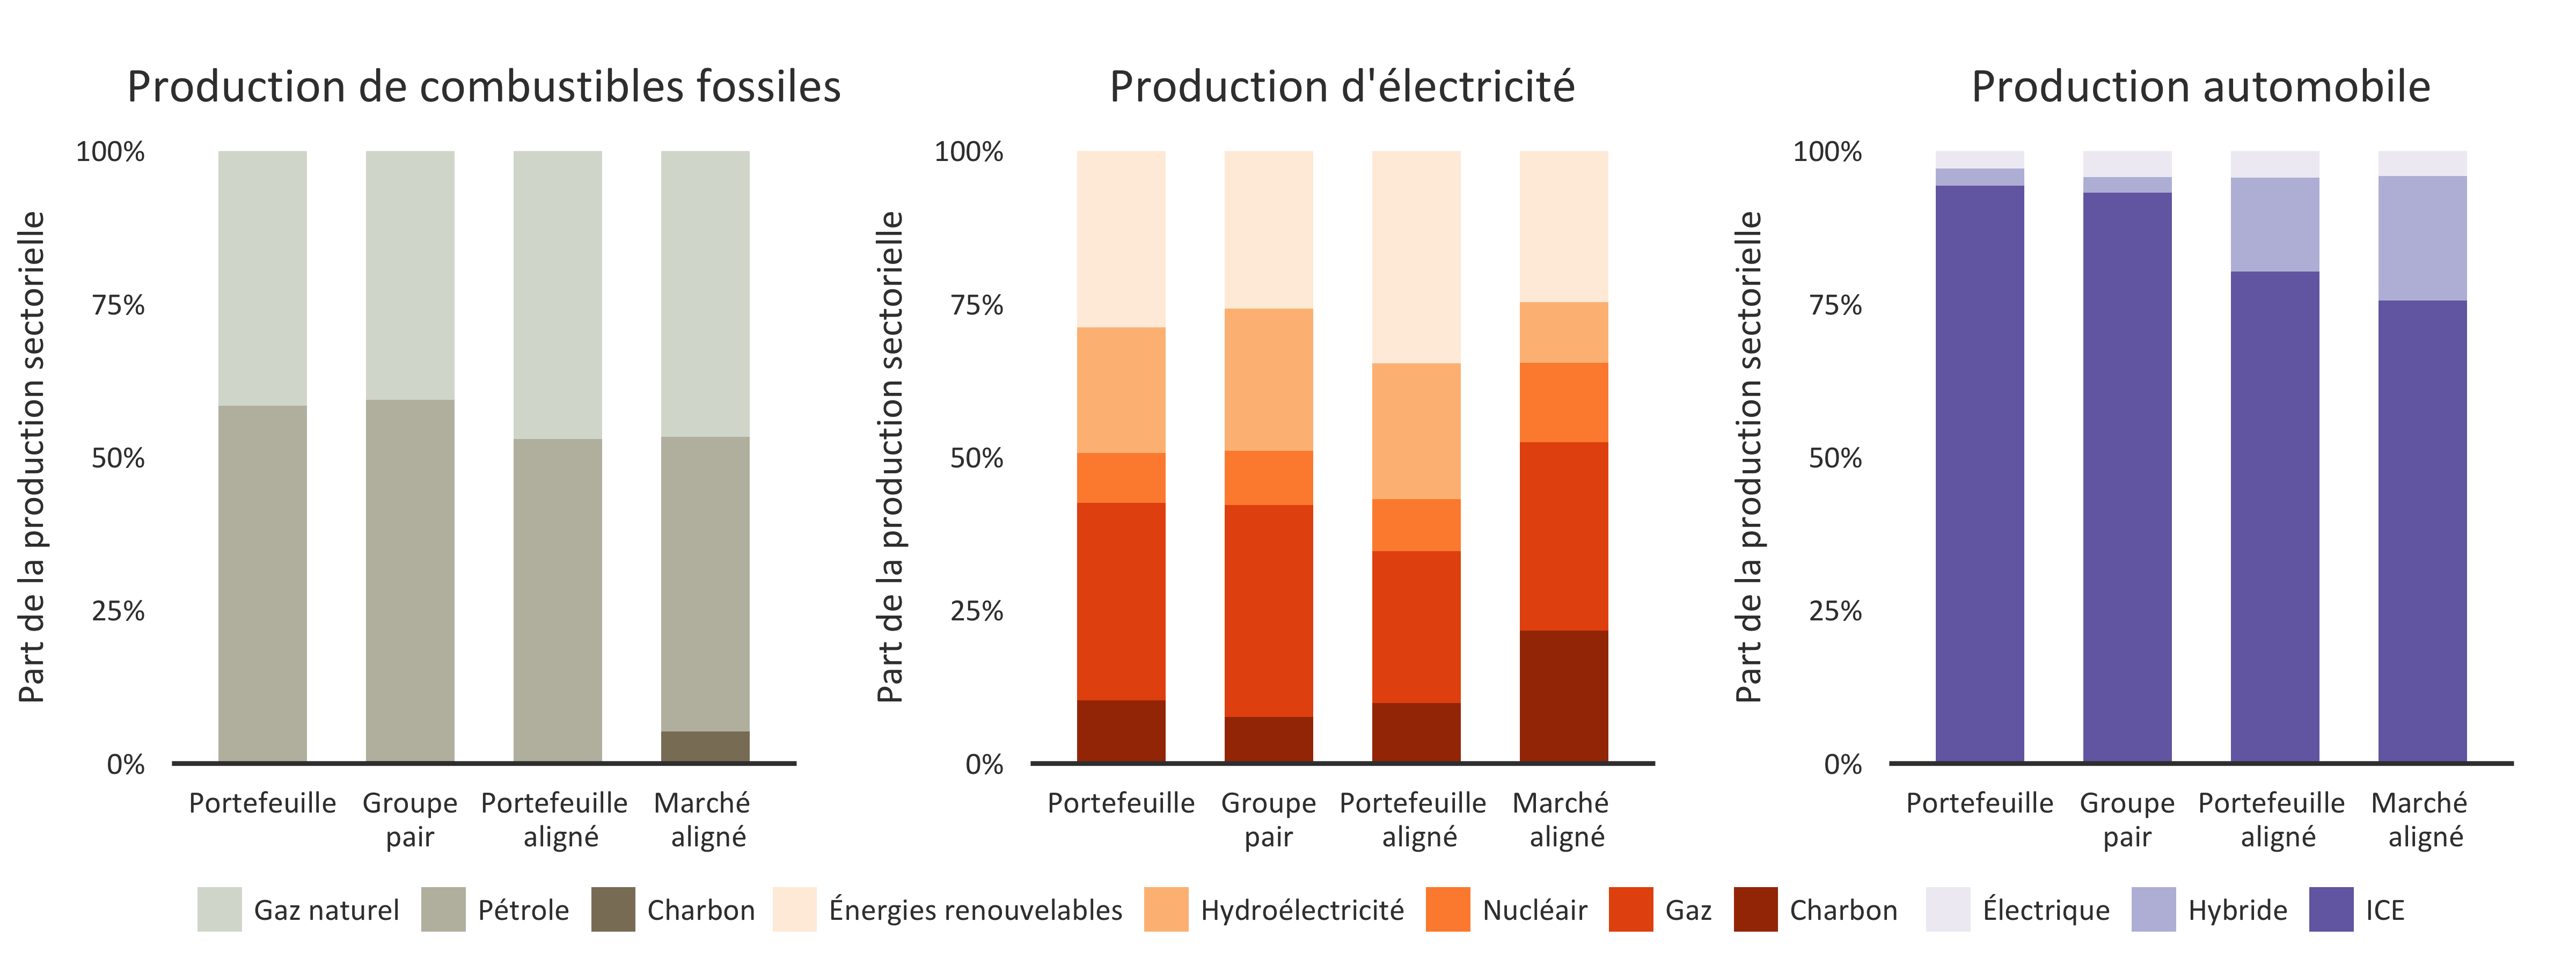
\includegraphics[trim = {0 0cm 0 0},width=1\linewidth]{ReportOutputs/Fig06}
	\end{center}
	%EQSpecificE
	%\PageFooterFourth
\PageFooter{4 - EXPOSURE OF THE PORTFOLIO}

	\newpage	
	%EQSpecificE
	%IncRankingE
	%CoalMiningChartS	
	\section*{} % REGIONAL EXPOSURE		
	\HeaderDouble{REGIONAL EXPOSURE}{COAL MINING}
	
	\begin{multicols}{2}
		
		The following charts show the regional exposure of the corporate bond and equity portfolios to coal mining in Startyear+5.
		
		This is the aggregation of coal mining allocated to the portfolio in each region. 
		
	\end{multicols}	
	
	%CBSpecificS
	\textbf{Regional exposure of the corporate bond portfolio to coal mining}
	\vspace{-.0cm}
	
	\begin{center}
		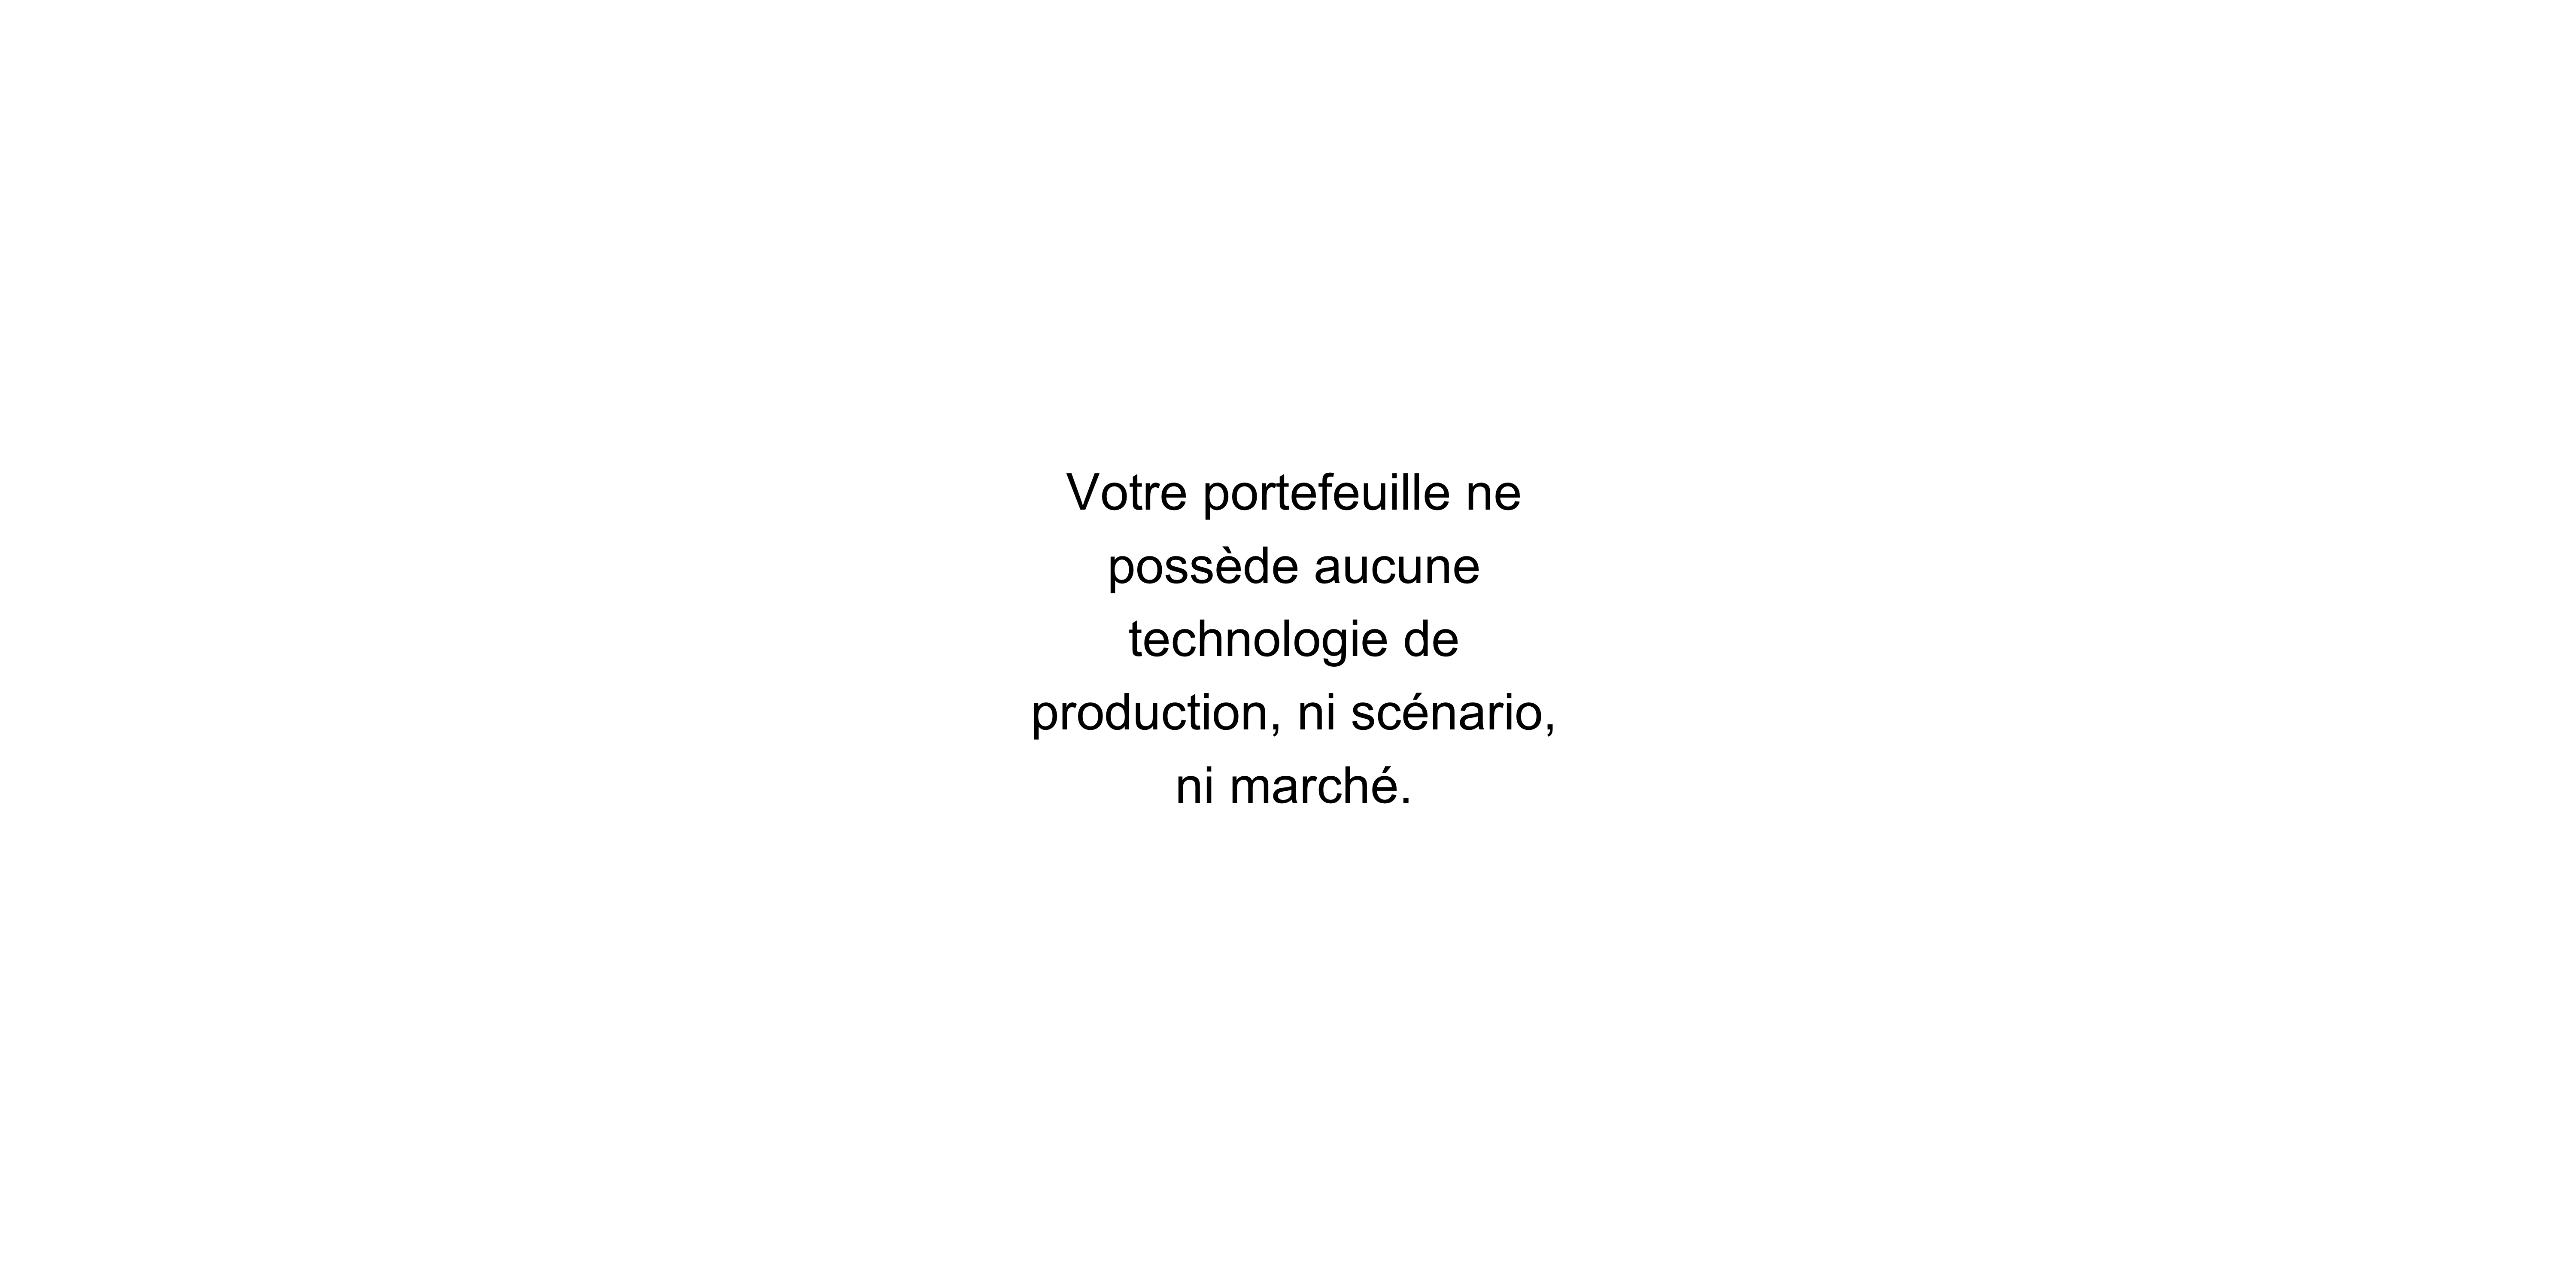
\includegraphics[trim = {2pt 2pt 2pt 2pt},clip,width=.9\linewidth]{ReportOutputs/Fig49}
	\end{center} 
	%CBSpecificE
	
	%EQSpecificS
	\textbf{Regional exposure of the equity portfolio to coal mining}
	\vspace{-.0cm}
	
	\begin{center}
		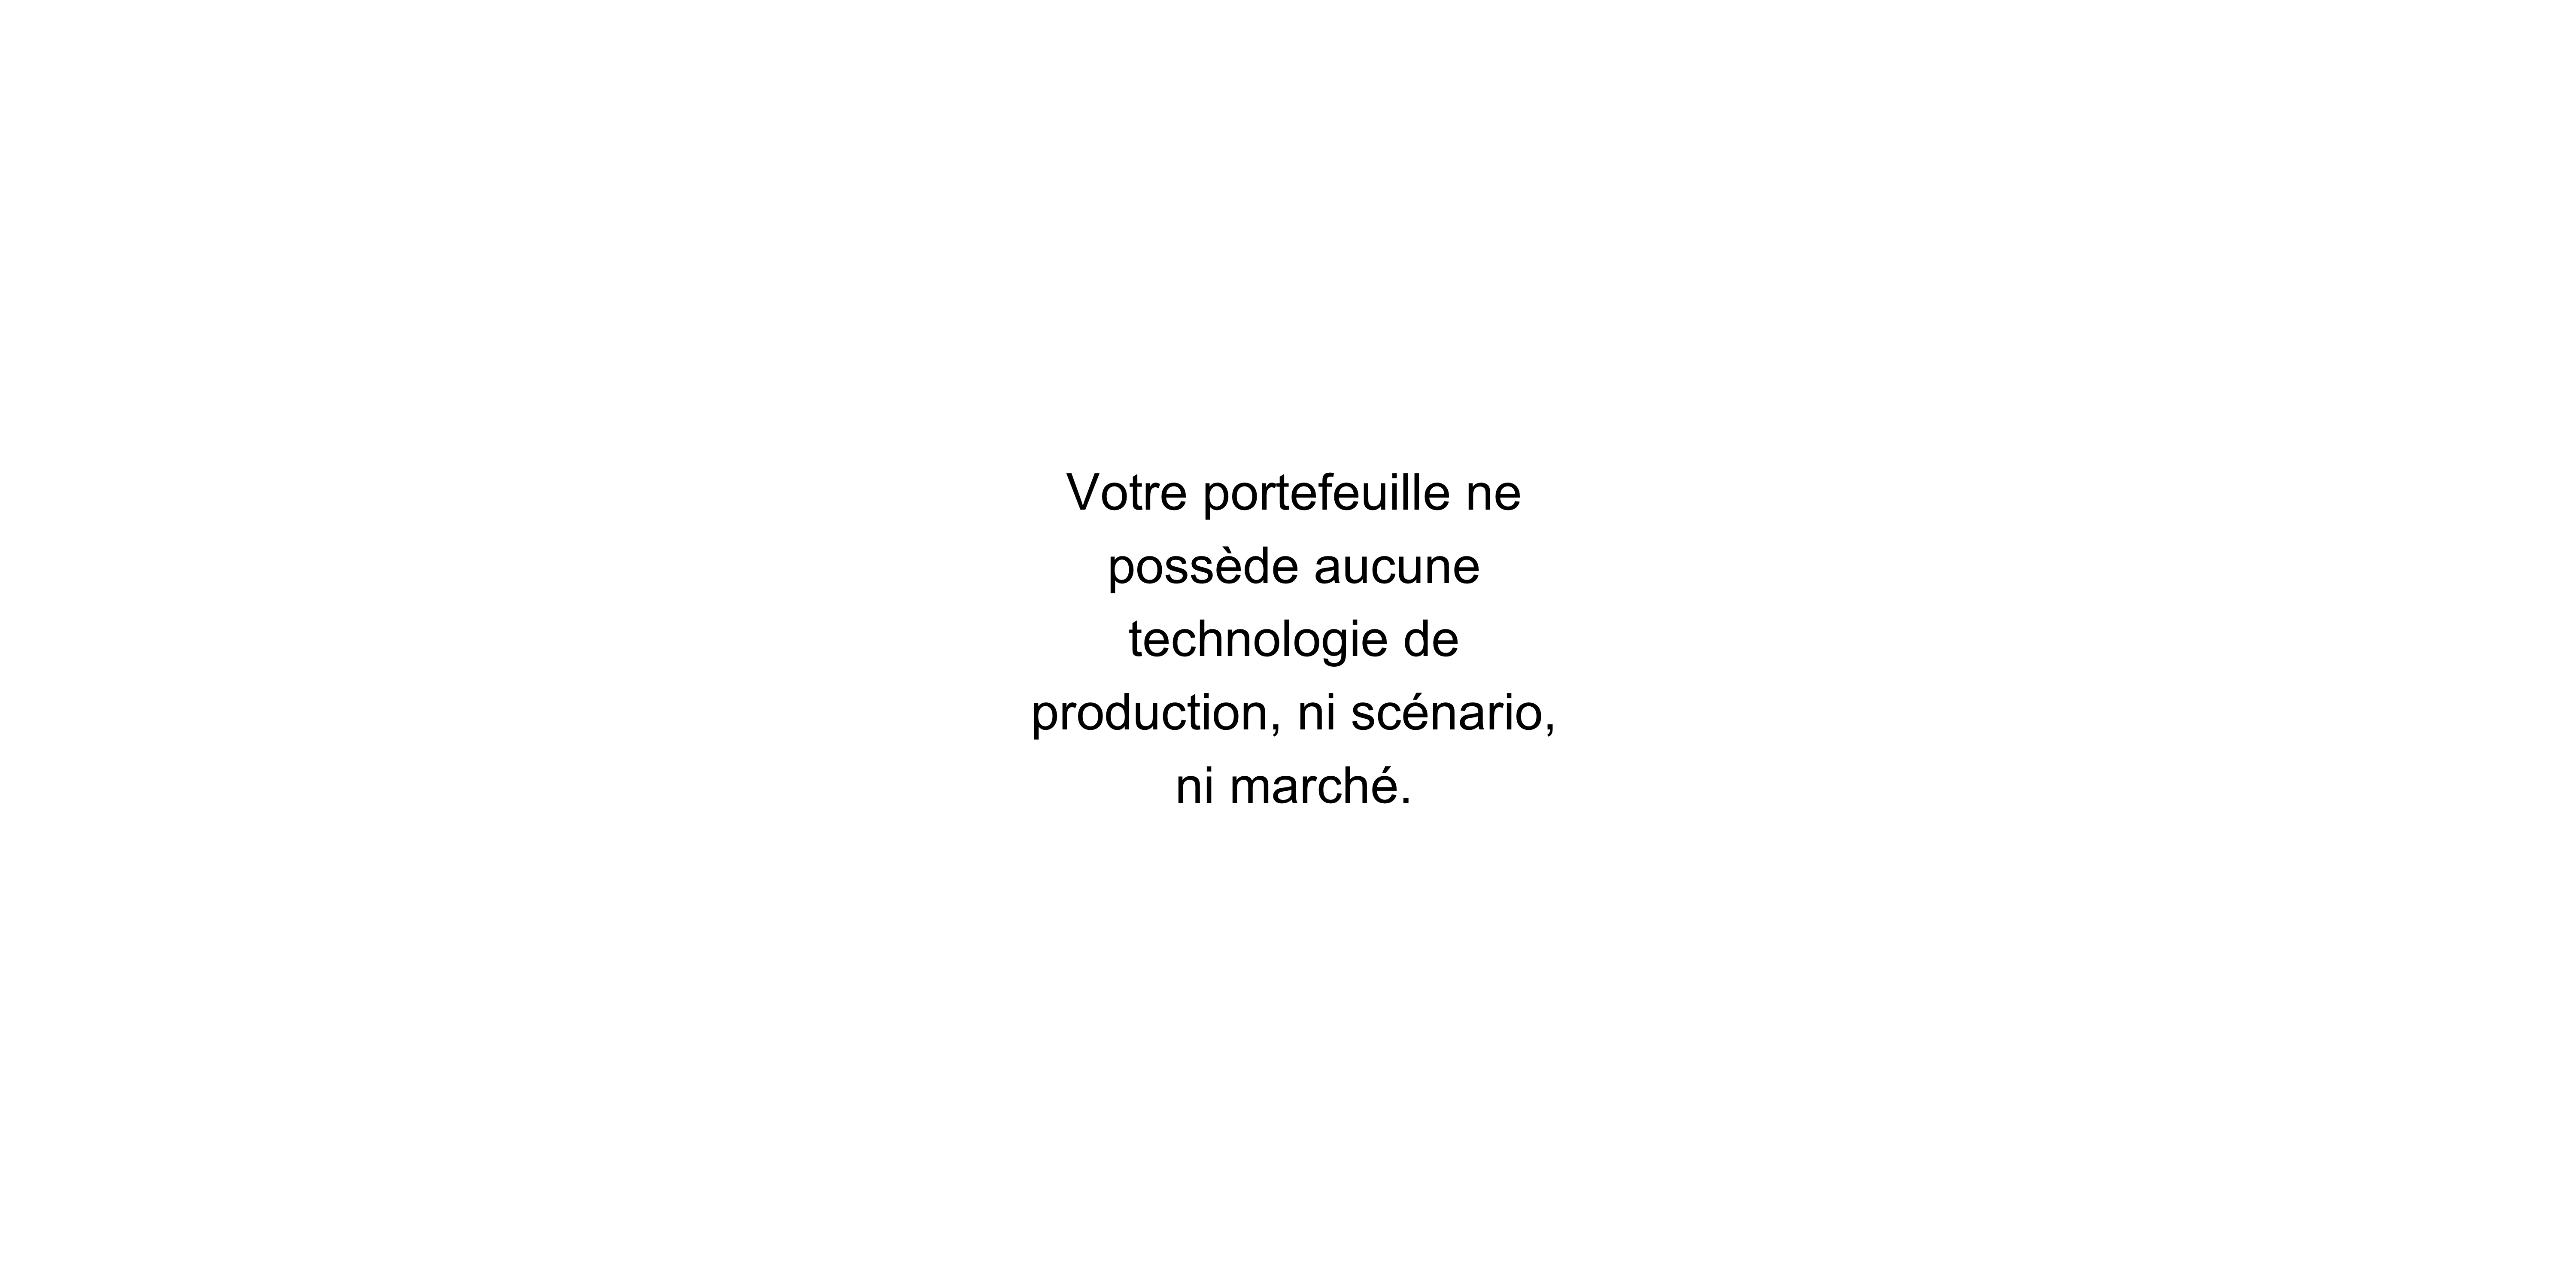
\includegraphics[trim = {1pt 1pt 1pt 1pt},width=.9\linewidth]{ReportOutputs/Fig50}
	\end{center} 
	%EQSpecificE
	
	%\PageFooterFourth
\PageFooter{4 - EXPOSURE OF THE PORTFOLIO}
	
	\newpage
	\section*{} % 5th SECTION   
	\SectionHeading{SECTION 5:}{COMPANY EXPOSURE}
	
	\newpage
	%CoalMiningChartE
	%CompanyChartsS
	\section*{} % CONTRIBUTIONS OF SECURITIES TO THE RESULTS 
	\HeaderSingle{CONTRIBUTIONS OF SECURITIES TO THE RESULTS}
	
	\begin{multicols}{2}
		
		\textbf{The objective of this section is to provide insight into the specific companies driving the results presented in the previous sections.}
		
		The following pages will show results for individual companies in the fossil fuel, power, and automotive sectors. The analytics provided show just one piece of information related to potential scenario analysis of companies and their contribution to a portfolio's performance. A range of additional indicators could be considered that go beyond the scope of this particular report. The indicators presented here should not be considered as investment recommendations, but rather as information about the companies driving the results of the portfolio scenario analysis. Section 6 provides further detail on the data sources informing this section. 
		
		As part of a partnership with a range of technical experts, 2Dii is currently developing a company scenario analysis report mirroring the portfolio reports presented here, designed to be made freely available and provide a more comprehensive and holistic picture of a company's positioning relative to a decarbonization scenario. This infrastructure can be used to inform future scenario analysis and actions and will be launched in the second half of 2018. The analytics in this report thus only show a snapshot of the type of data that can be explored. 
		
		The following will briefly summarize the type of data that is shown for each sector that is present in the portfolio. 
		
		\textbf{Oil and gas.} For oil and gas production, three types of indicators are shown. 
		
		\begin{enumerate}
			\item The first indicator is the total planned change in production of oil and gas companies over the next 5 years, based on the currently revealed production plans in the asset-level databases. The graphs on the next page show the largest companies by amount of oil or gas production allocated to the corporate bond and equity portfolios in Startyear; these companies have the most influence on the portfolio's alignment results for the fossil fuels sector. For each asset class and technology, the results are shown relative to the portfolio's targeted total change in production during the 5 year period under the ScenarioValue (green bar). It should be noted that the figures provided are based on current estimated production and evolution of the existing asset base. Mergers, acquisitions, and increases in capital expenditure relative to baselines may of course lead to changes in these trends over time. 
			\item The second indicator builds on analysis conducted by the Carbon Tracker Initiative in partnership with the UN Principles for Responsible Investment (UNPRI). This indicator takes a more long-term view and analyses the alignment of companies with a 2\degree C carbon budget from the perspective of the cost structure of their oil and gas assets. This indicator differs from the first in terms of the time horizon and the underlying allocation rules that allocate macro scenarios to microeconomic actors. More information on the methodology and the approach can be found at http://www.2degreeseparation.com/. This indicator can only be used to analyze the listed equity portfolio, as data is unavailable for corporate bond securities. 
			\item The third indicator shows the breakdown of oil assets of individual companies by type of oil (e.g., conventional, tar sands, etc.). Wood Mackenzie (2018) proposes that while shifting away from high-carbon fuels towards low carbon is necessary as an overall trend, within the oil and gas industry, shifting away from particular extraction methods is a transitional alternative. This report does not comment on the emissions by extraction type, however data is available on this. Investors need to look beyond resource themes and review the variations in upstream emissions intensity to see how companies can reduce their carbon footprints. Even assets of the same theme can have significantly different emissions intensity based upon maturity, location and other unique factors.
		\end{enumerate}
			
		\textbf{Power and automotive sectors.} For the power and automotive sectors, the company level information focuses on the technology mix of the utilities and automotive manufacturers in the corporate bond and equity portfolios, informing in particular the results for Section 4. Additional information on the build out plans of these companies and the changes over time can be provided upon request. 
		
		%CBSpecificS
		\textit{Please note, for the corporate bond portfolio, the results are provided at debt ticker level. This is because a single debt ticker could be associated with multiple companies.}
		%CBSpecificE
		
	\end{multicols}
	
	%\PageFooterFifth
\PageFooter{5 - COMPANY EXPOSURE}
	
	\newpage
	%FossilFuelSector_ALLS
	\section*{} % CONTRIBUTIONS OF SECURITIES TO THE RESULTS 
	\HeaderDouble{CONTRIBUTIONS OF SECURITIES TO THE RESULTS}{OIL AND GAS - CORPORATE BONDS} 
	
	%FossilFuelSector_CBS
	\vspace{-.05cm}
	\textbf{Planned changes in oil and gas production of companies with most production allocated to the corporate bond portfolio in Startyear+5.} This graph shows the planned increases and decreases in production for gas and oil for the largest companies in this sector in the corporate bond portfolio over the next five years. This is compared to the required change as per the ScenarioValue. 
	\vspace{-.15cm}
	
	\begin{center}
		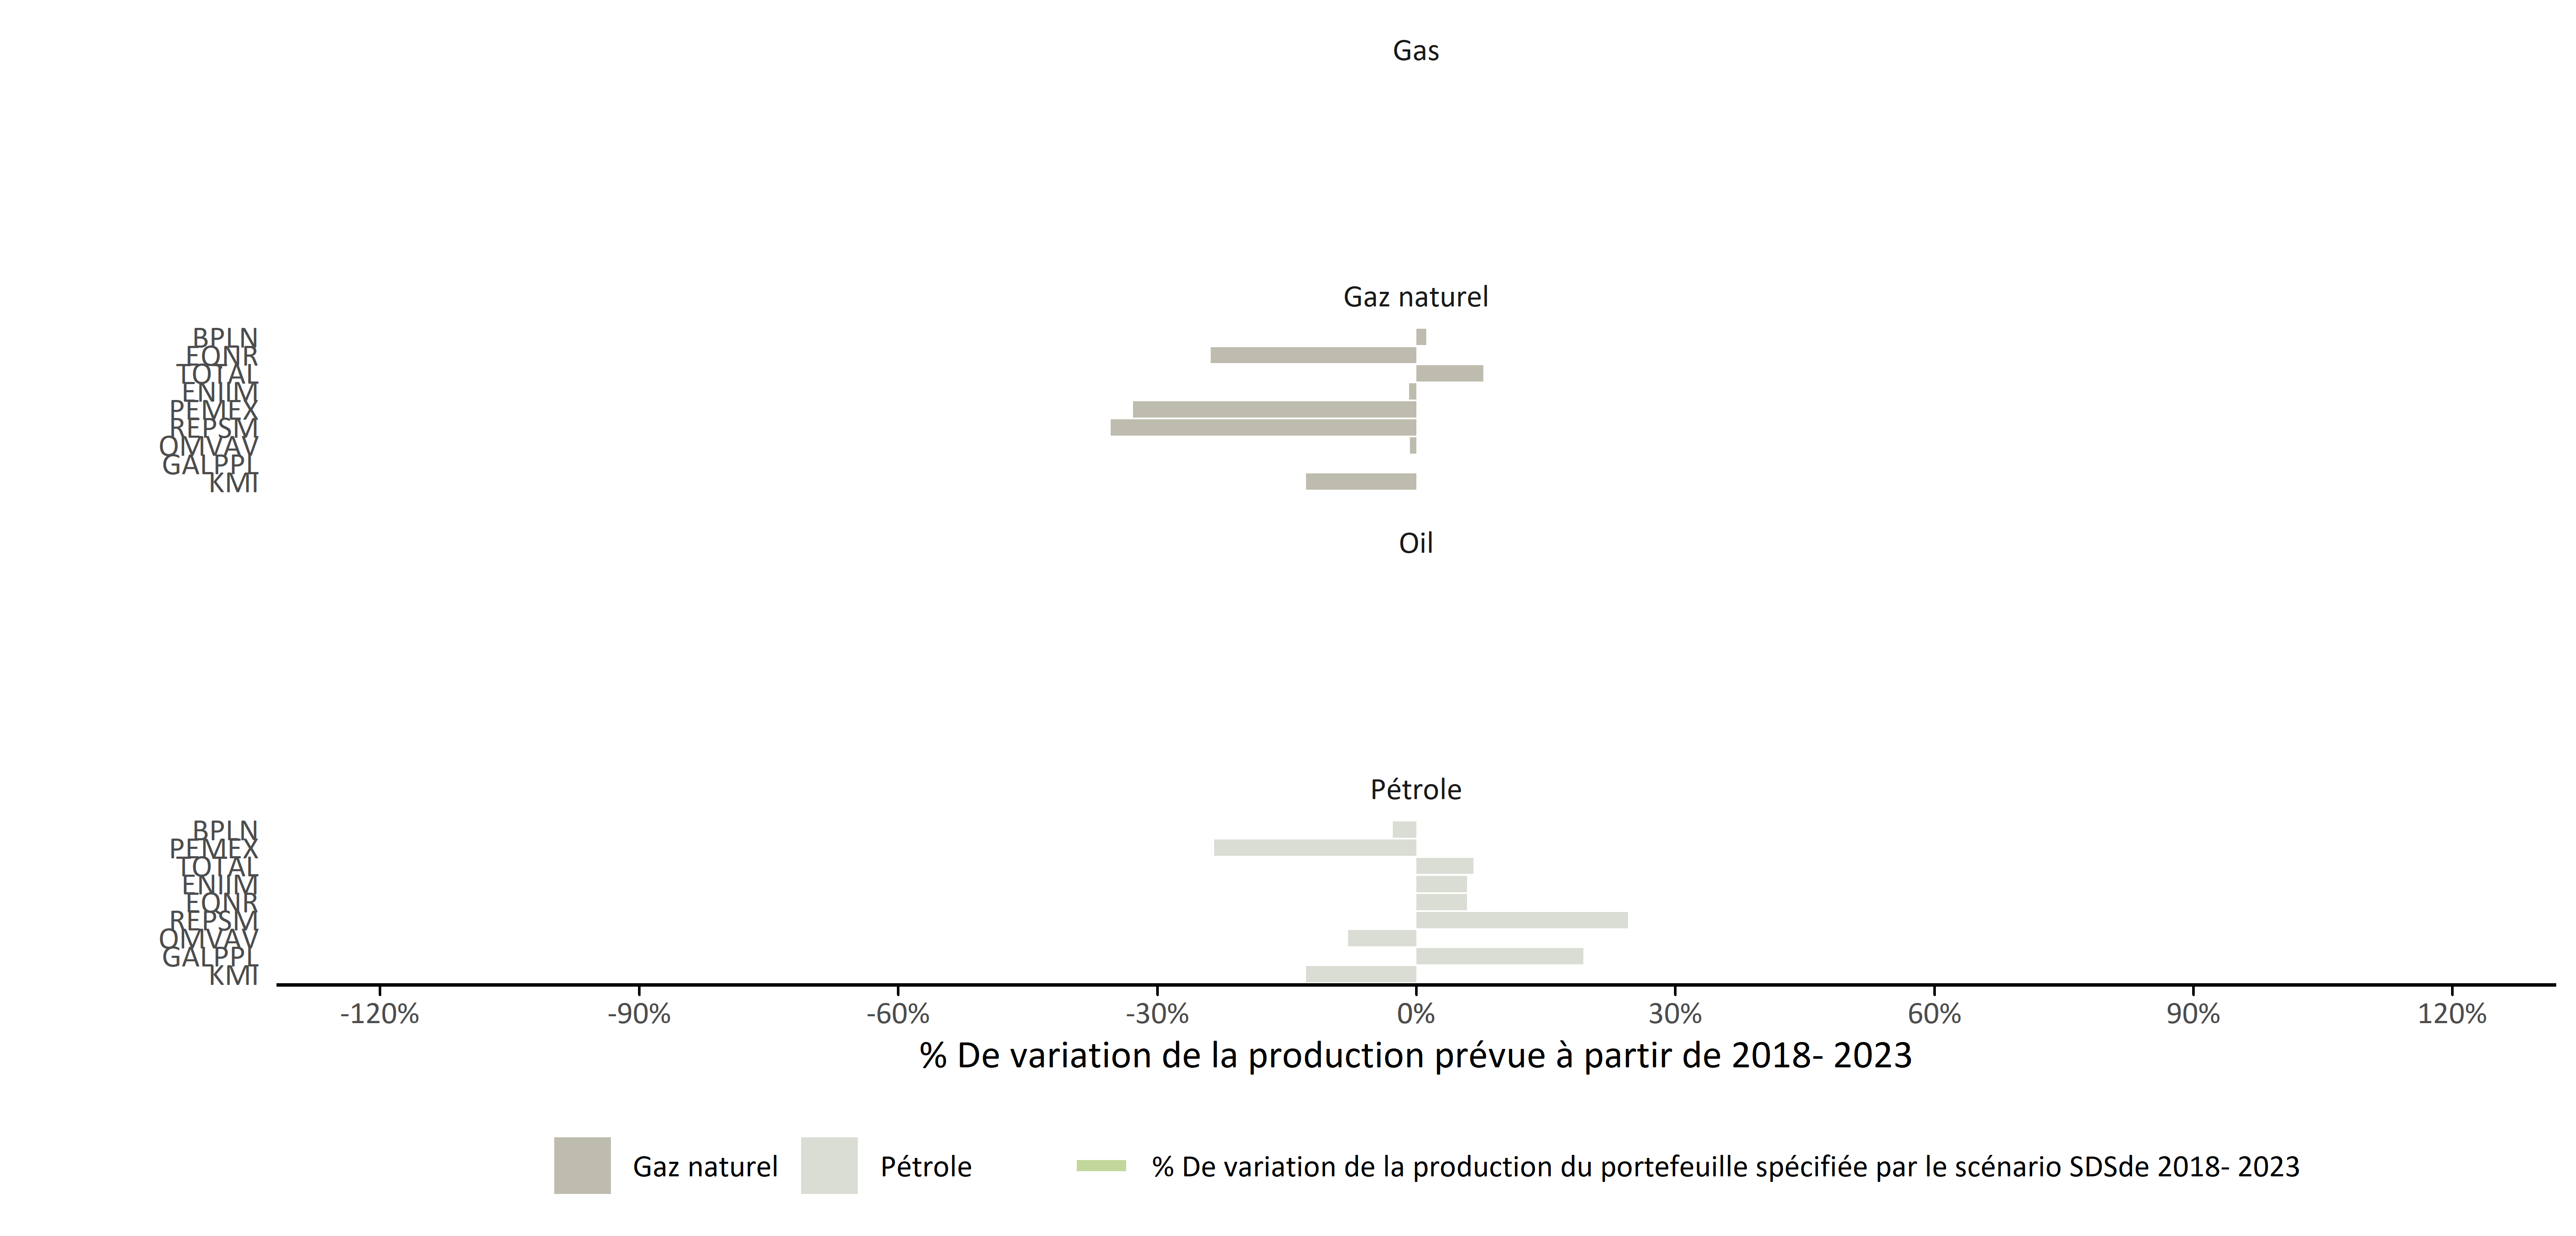
\includegraphics[trim = {0 0cm 0 0},width=1\linewidth]{ReportOutputs/Fig42}
	\end{center}
	%FossilFuelSector_CBE
	%FossilFuelSector_EQS
	
\PageFooter{5 - COMPANY EXPOSURE}

\newpage
%FossilFuelSector_ALLS
\section*{} % CONTRIBUTIONS OF SECURITIES TO THE RESULTS 
\HeaderDouble{CONTRIBUTIONS OF SECURITIES TO THE RESULTS}{OIL AND GAS - EQUITY} 
	
	\textbf{Planned changes in oil and gas production of companies with most production allocated to the equity portfolio in Startyear+5.} This graph shows the planned increases and decreases in production for gas and oil for the largest companies in this sector in the equity portfolio over the next five years. This is compared to the required change as per the ScenarioValue. 
	\vspace{-.35cm}
	
	\begin{center}
		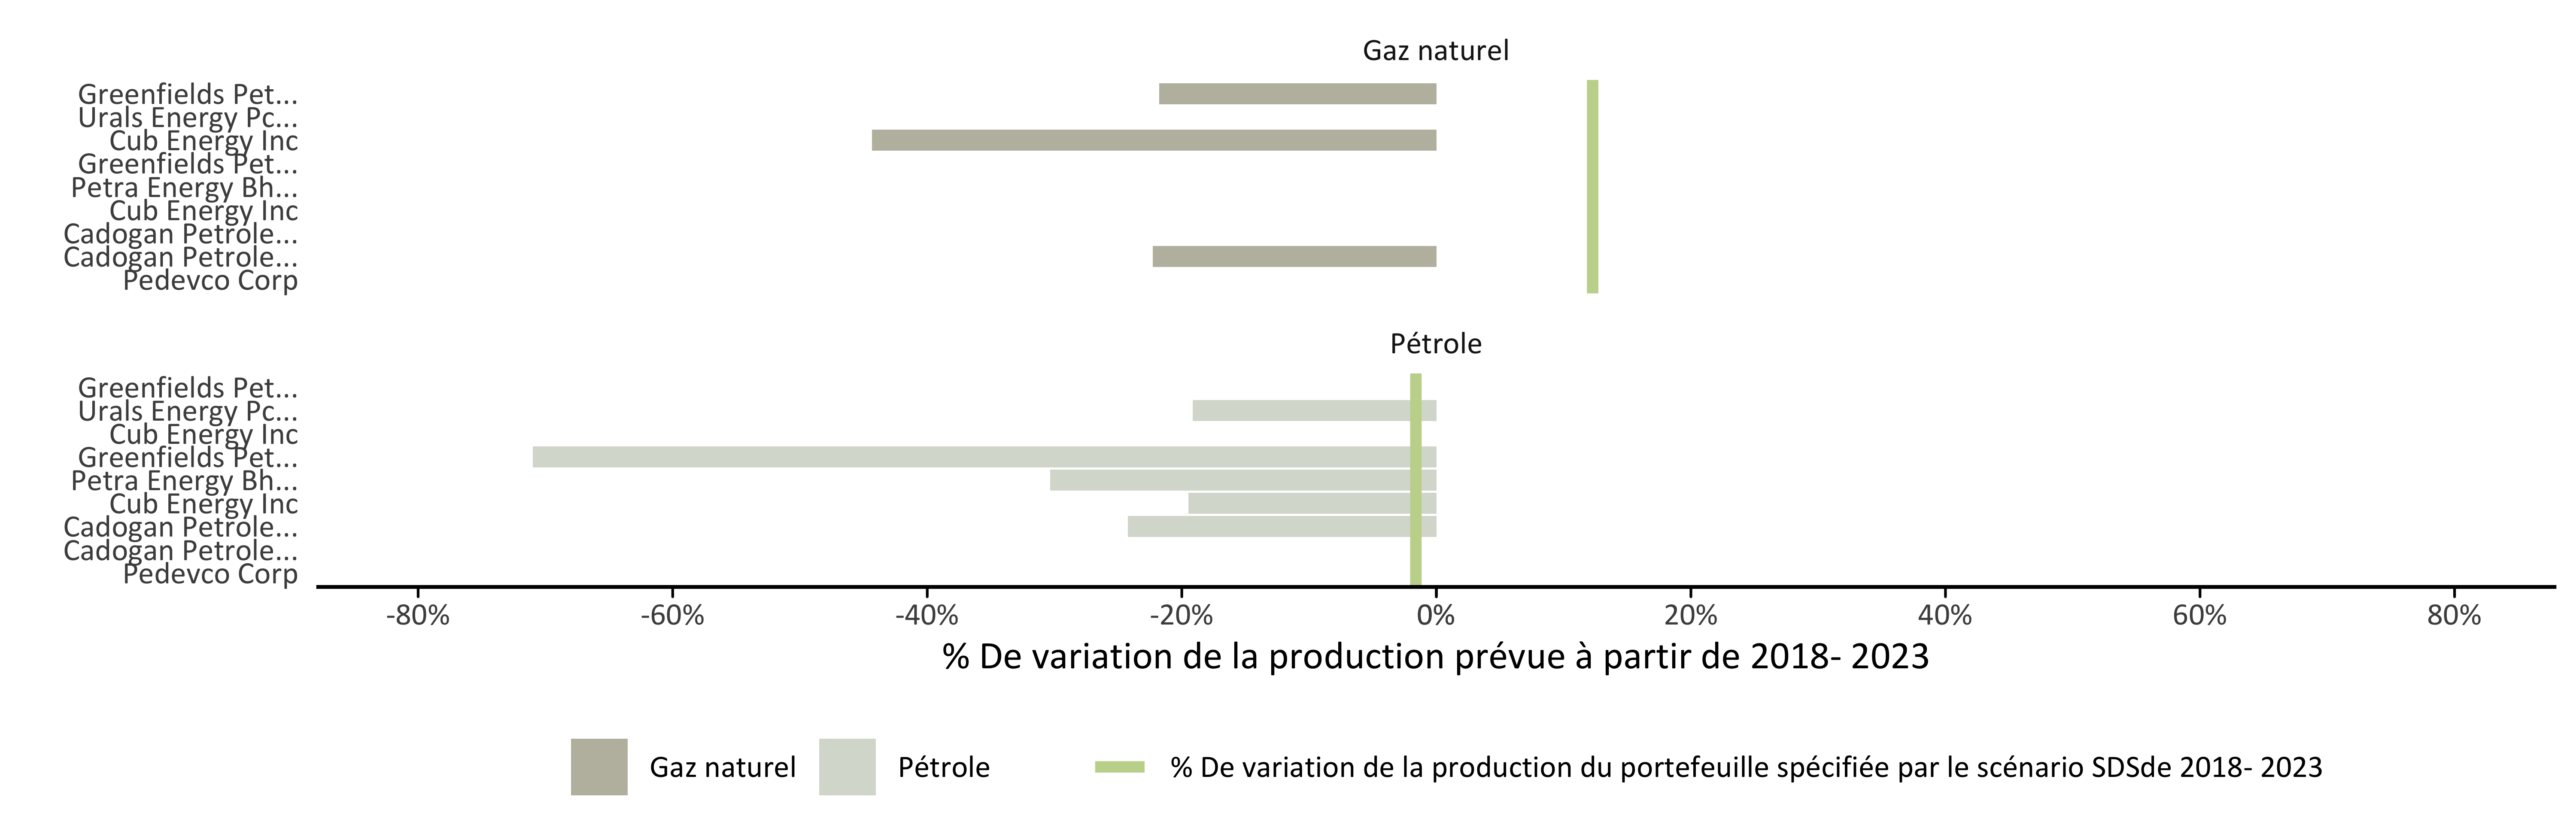
\includegraphics[trim = {0 0cm 0 0},width=1\linewidth]{ReportOutputs/Fig46}
	\end{center}
	\vspace{-.5cm}
	%\begin{center}
	%	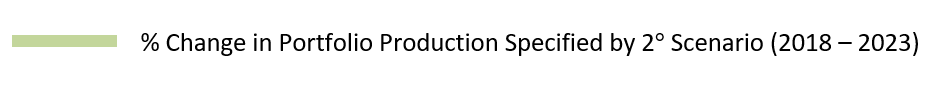
\includegraphics[trim = {0 0cm 0 0},width=.5\linewidth]{ReportGraphics/ogLegend.png}
	%\end{center}
	%FossilFuelSector_EQE
	
	%FossilFuelOneSectorS
	%\PageFooterFifth
\PageFooter{5 - COMPANY EXPOSURE}
	
	\newpage
	
	\section*{} % CONTRIBUTIONS OF SECURITIES TO THE RESULTS
	\HeaderDouble{CONTRIBUTIONS OF SECURITIES TO THE RESULTS}{OIL AND GAS}
	%FossilFuelOneSectorE
	
	%CarbonBudgetS
	\textbf{Carbon budget alignment of the largest oil companies in the equity portfolio in Startyear+5.} This graph is based on the work of the Carbon Tracker Initiative and shows the carbon budget alignment, and by extension the level of potential exposure to unneeded capex, of the largest oil and gas producers (by market value). 
	
	\vspace{-.35cm}
	
	\begin{center}
		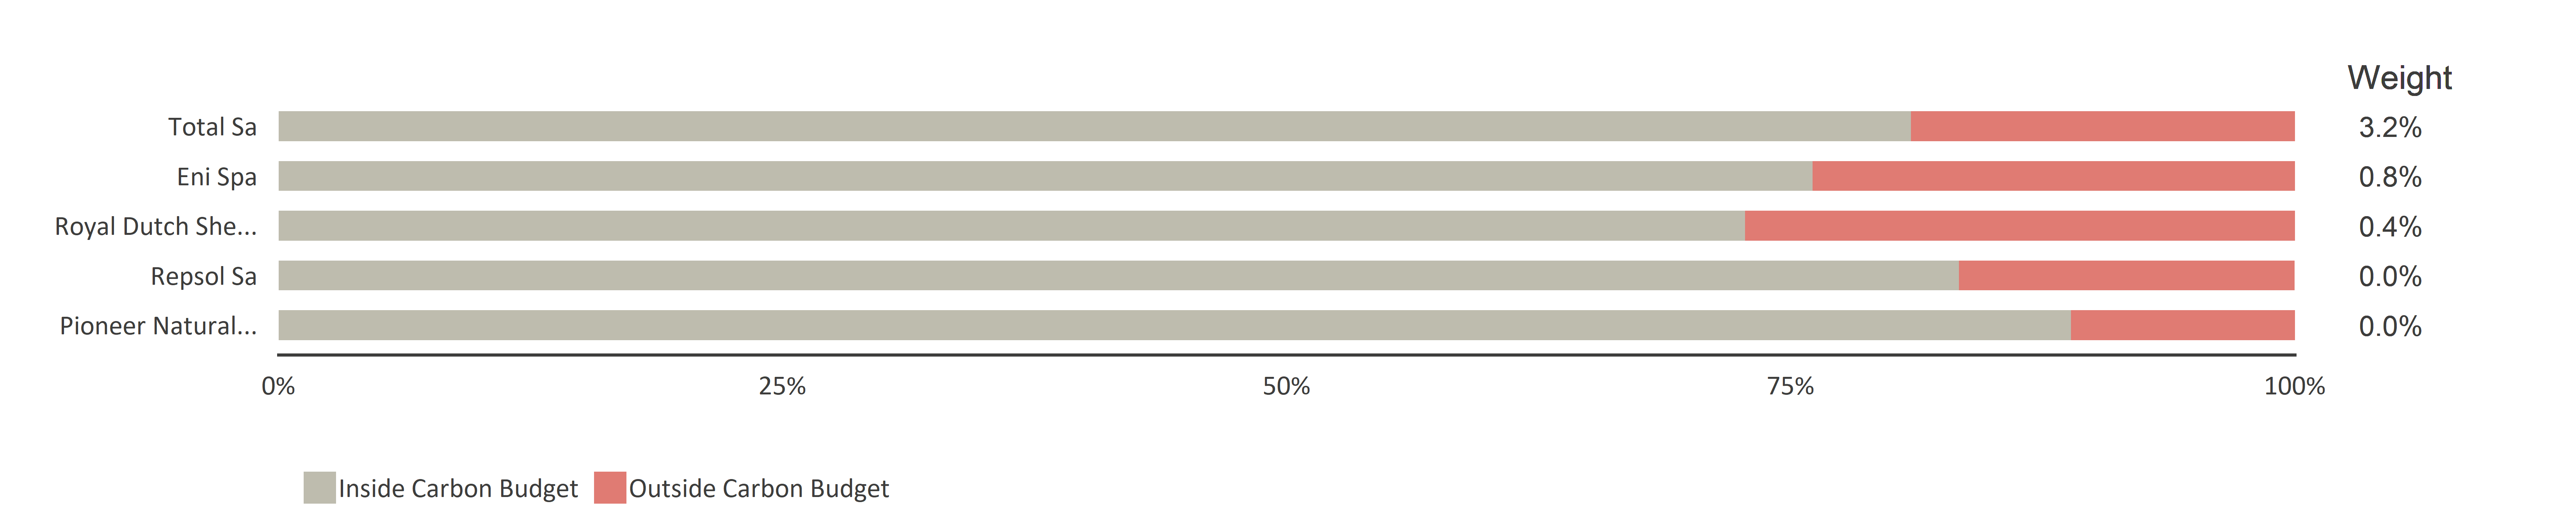
\includegraphics[trim = {0 0cm 0 0},width=1\linewidth]{ReportOutputs/Fig48}
	\end{center}
	%CarbonBudgetE
	
	
	%FossilFuelSector_CBS
	\textbf{Resource breakdown of oil production of the largest holdings in the corporate bond portfolio in Startyear+5.}
	This graph shows oil production by type of oil for the largest holdings (by market value) of oil producers in the corporate bond portfolio. 
	
	\vspace{-.35cm}
	
	\begin{center}
		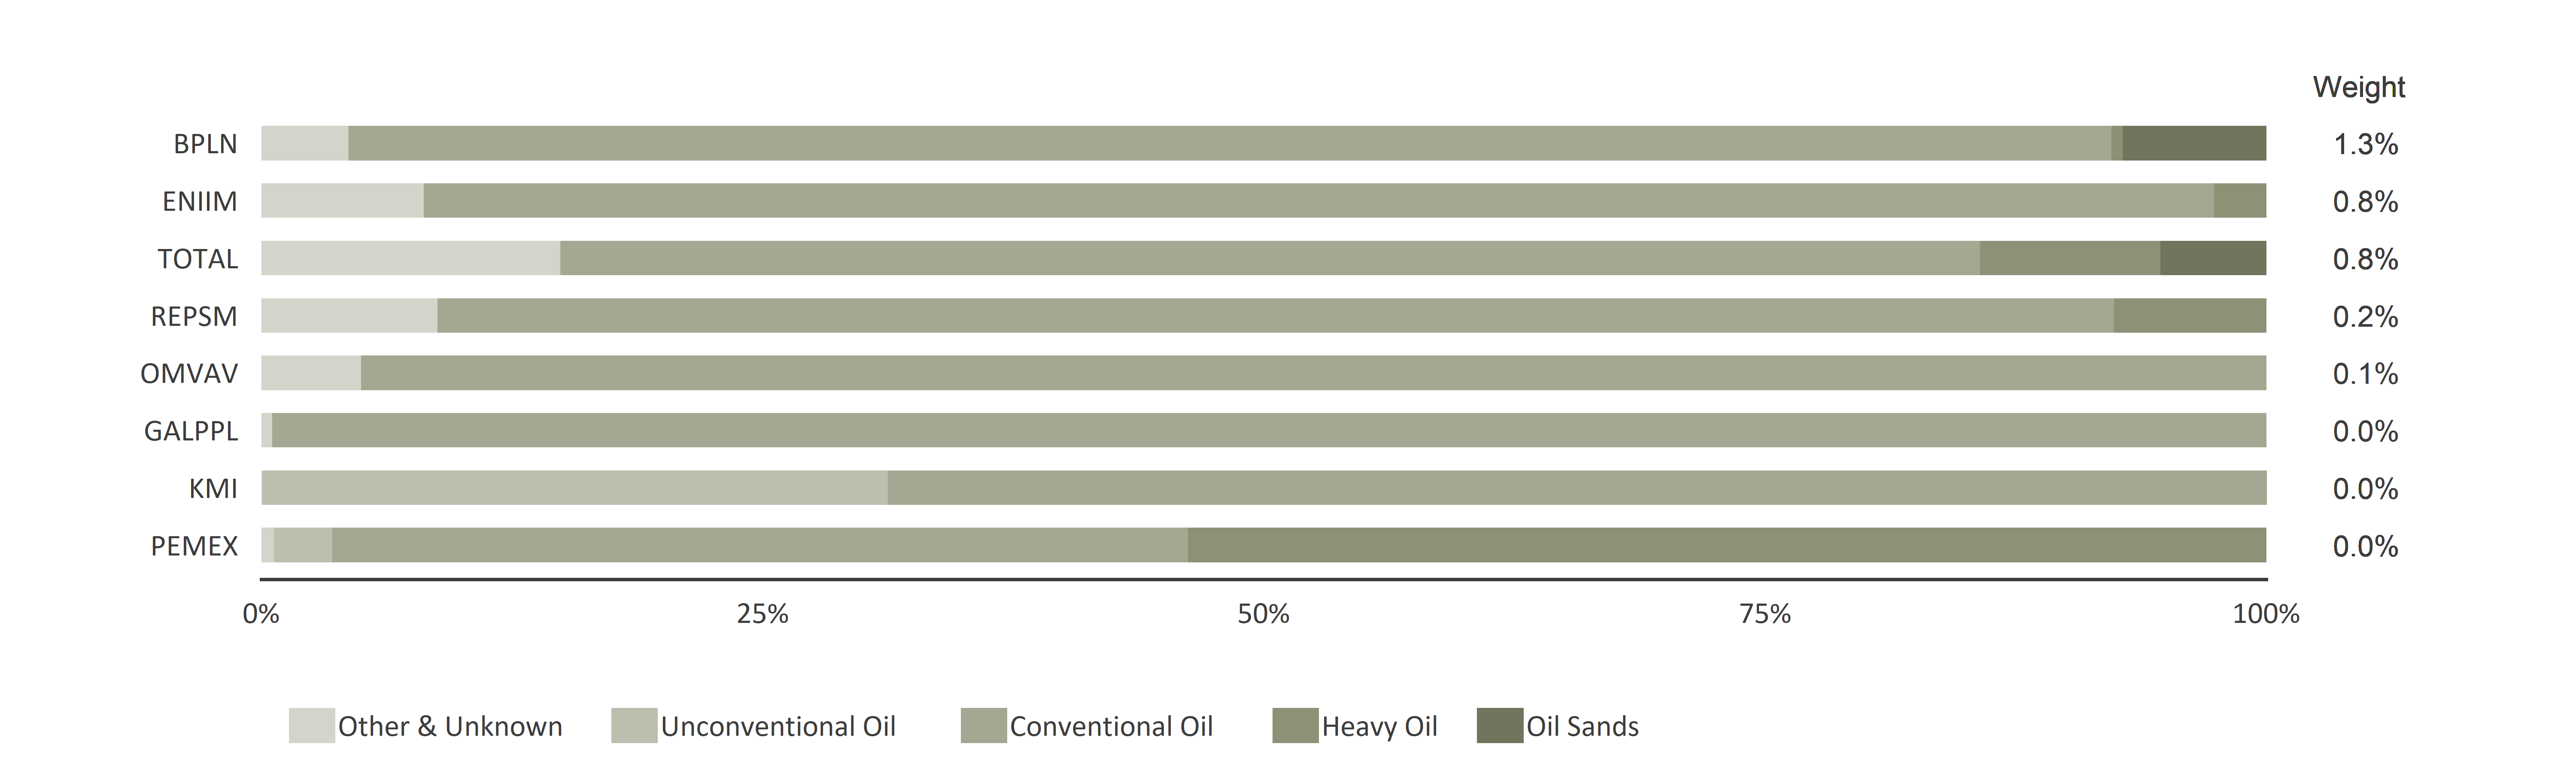
\includegraphics[trim = {0 0cm 0 0},width=1\linewidth]{ReportOutputs/Fig43}
	\end{center}
	%FossilFuelSector_CBE
	
	%FossilFuelSector_EQS
	\textbf{Resource breakdown of oil production of the largest holdings in the equity portfolio in Startyear+5.}
	This graph shows oil production by type of oil for the largest holdings (by market value) of oil producers in the equity portfolio. 
	
	\vspace{-.35cm}
	
	\begin{center}
		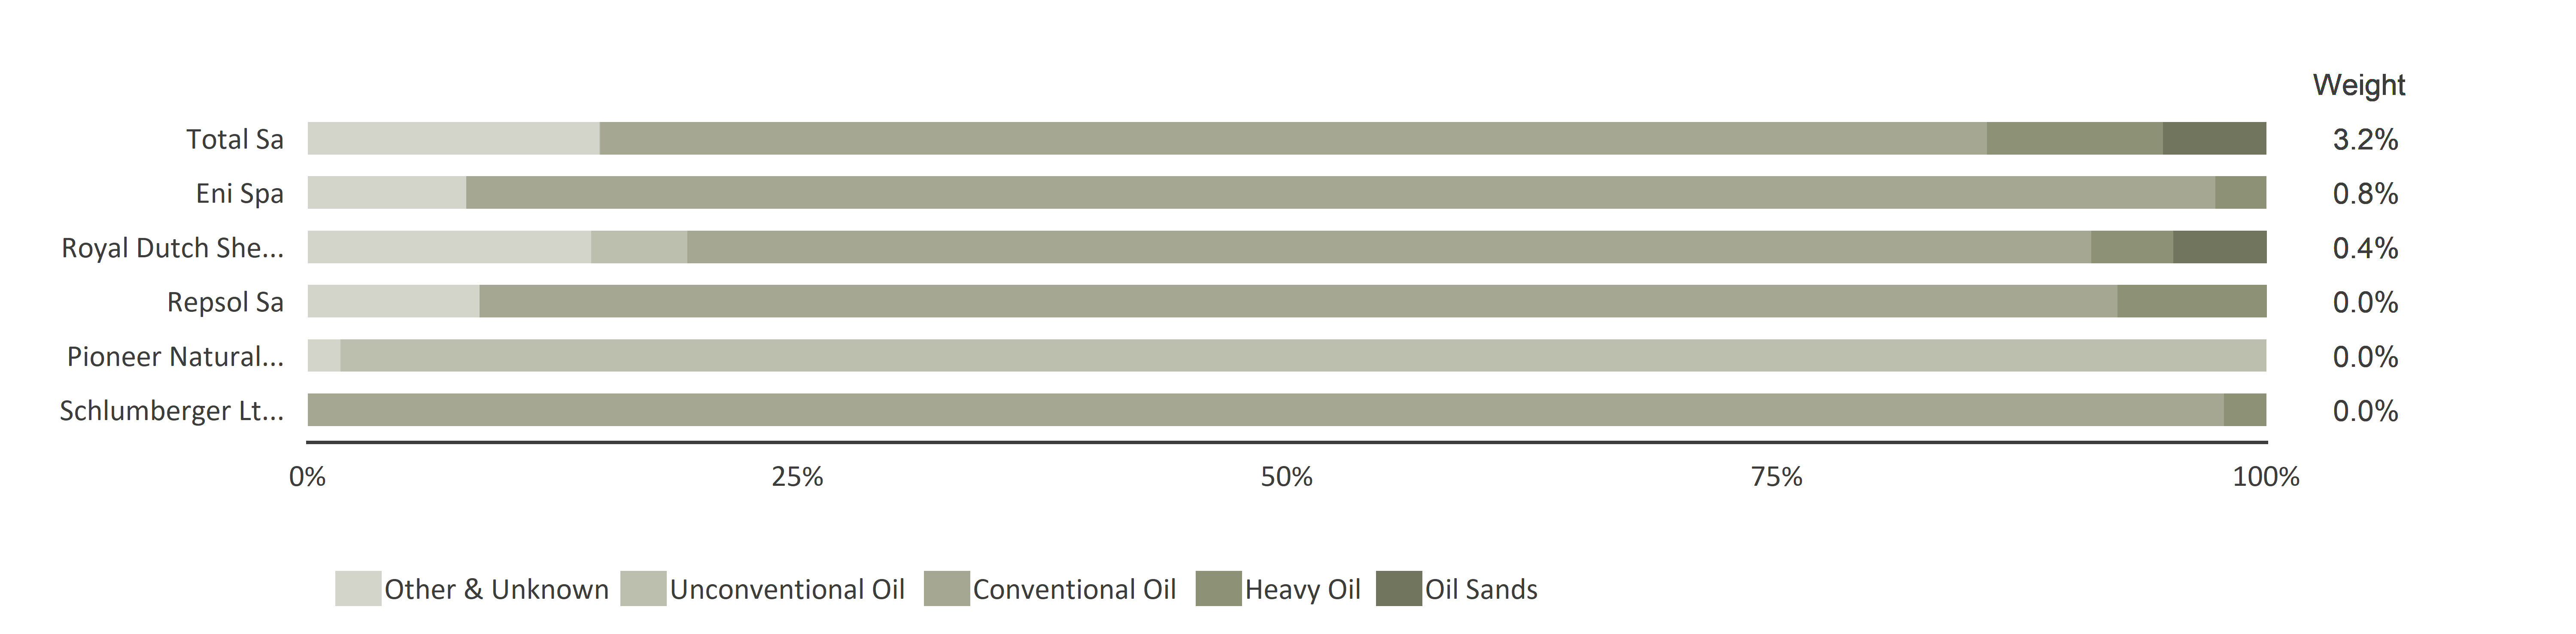
\includegraphics[trim = {0 0cm 0 0},width=1\linewidth]{ReportOutputs/Fig47}
	\end{center}


	%FossilFuelSector_EQE 
	%\PageFooterFifth
\PageFooter{5 - COMPANY EXPOSURE}
	
	\newpage

	
	%FossilFuelSector_ALLE
	
	
 	%PowerSector_ALLS
	\section*{} % CONTRIBUTIONS OF SECURITIES TO THE RESULTS
	%PowerAutoOneSectorS
	\HeaderDouble{CONTRIBUTIONS OF SECURITIES TO THE RESULTS}{POWER}
	%PowerAutoOneSectorE
	
	%PowerAutoTwoSectorsS
	\HeaderDouble{CONTRIBUTIONS OF SECURITIES TO THE RESULTS}{POWER AND AUTOMOTIVE}
	%PowerAutoTwoSectorsE
	
		\textbf{The figures below show the currently planned fuel mix in Startyear+5 for the largest holdings (by market value) of utilities in the corporate bond and equity portfolios.} 
		
		
		The results are shown compared to the portfolio's currently planned fuel mix, the portfolio's target fuel mix under the ScenarioValue, and the aligned market's fuel mix all as of Startyear+5. The weight is the size of the total investment in each company as a percent of the total value of the relevant portfolio. 
		
	
	%PowerSector_CBS
	\textbf{Technology breakdown of power companies within the corporate bond portfolio}
	\vspace{-.0cm}
	
	\begin{center}
		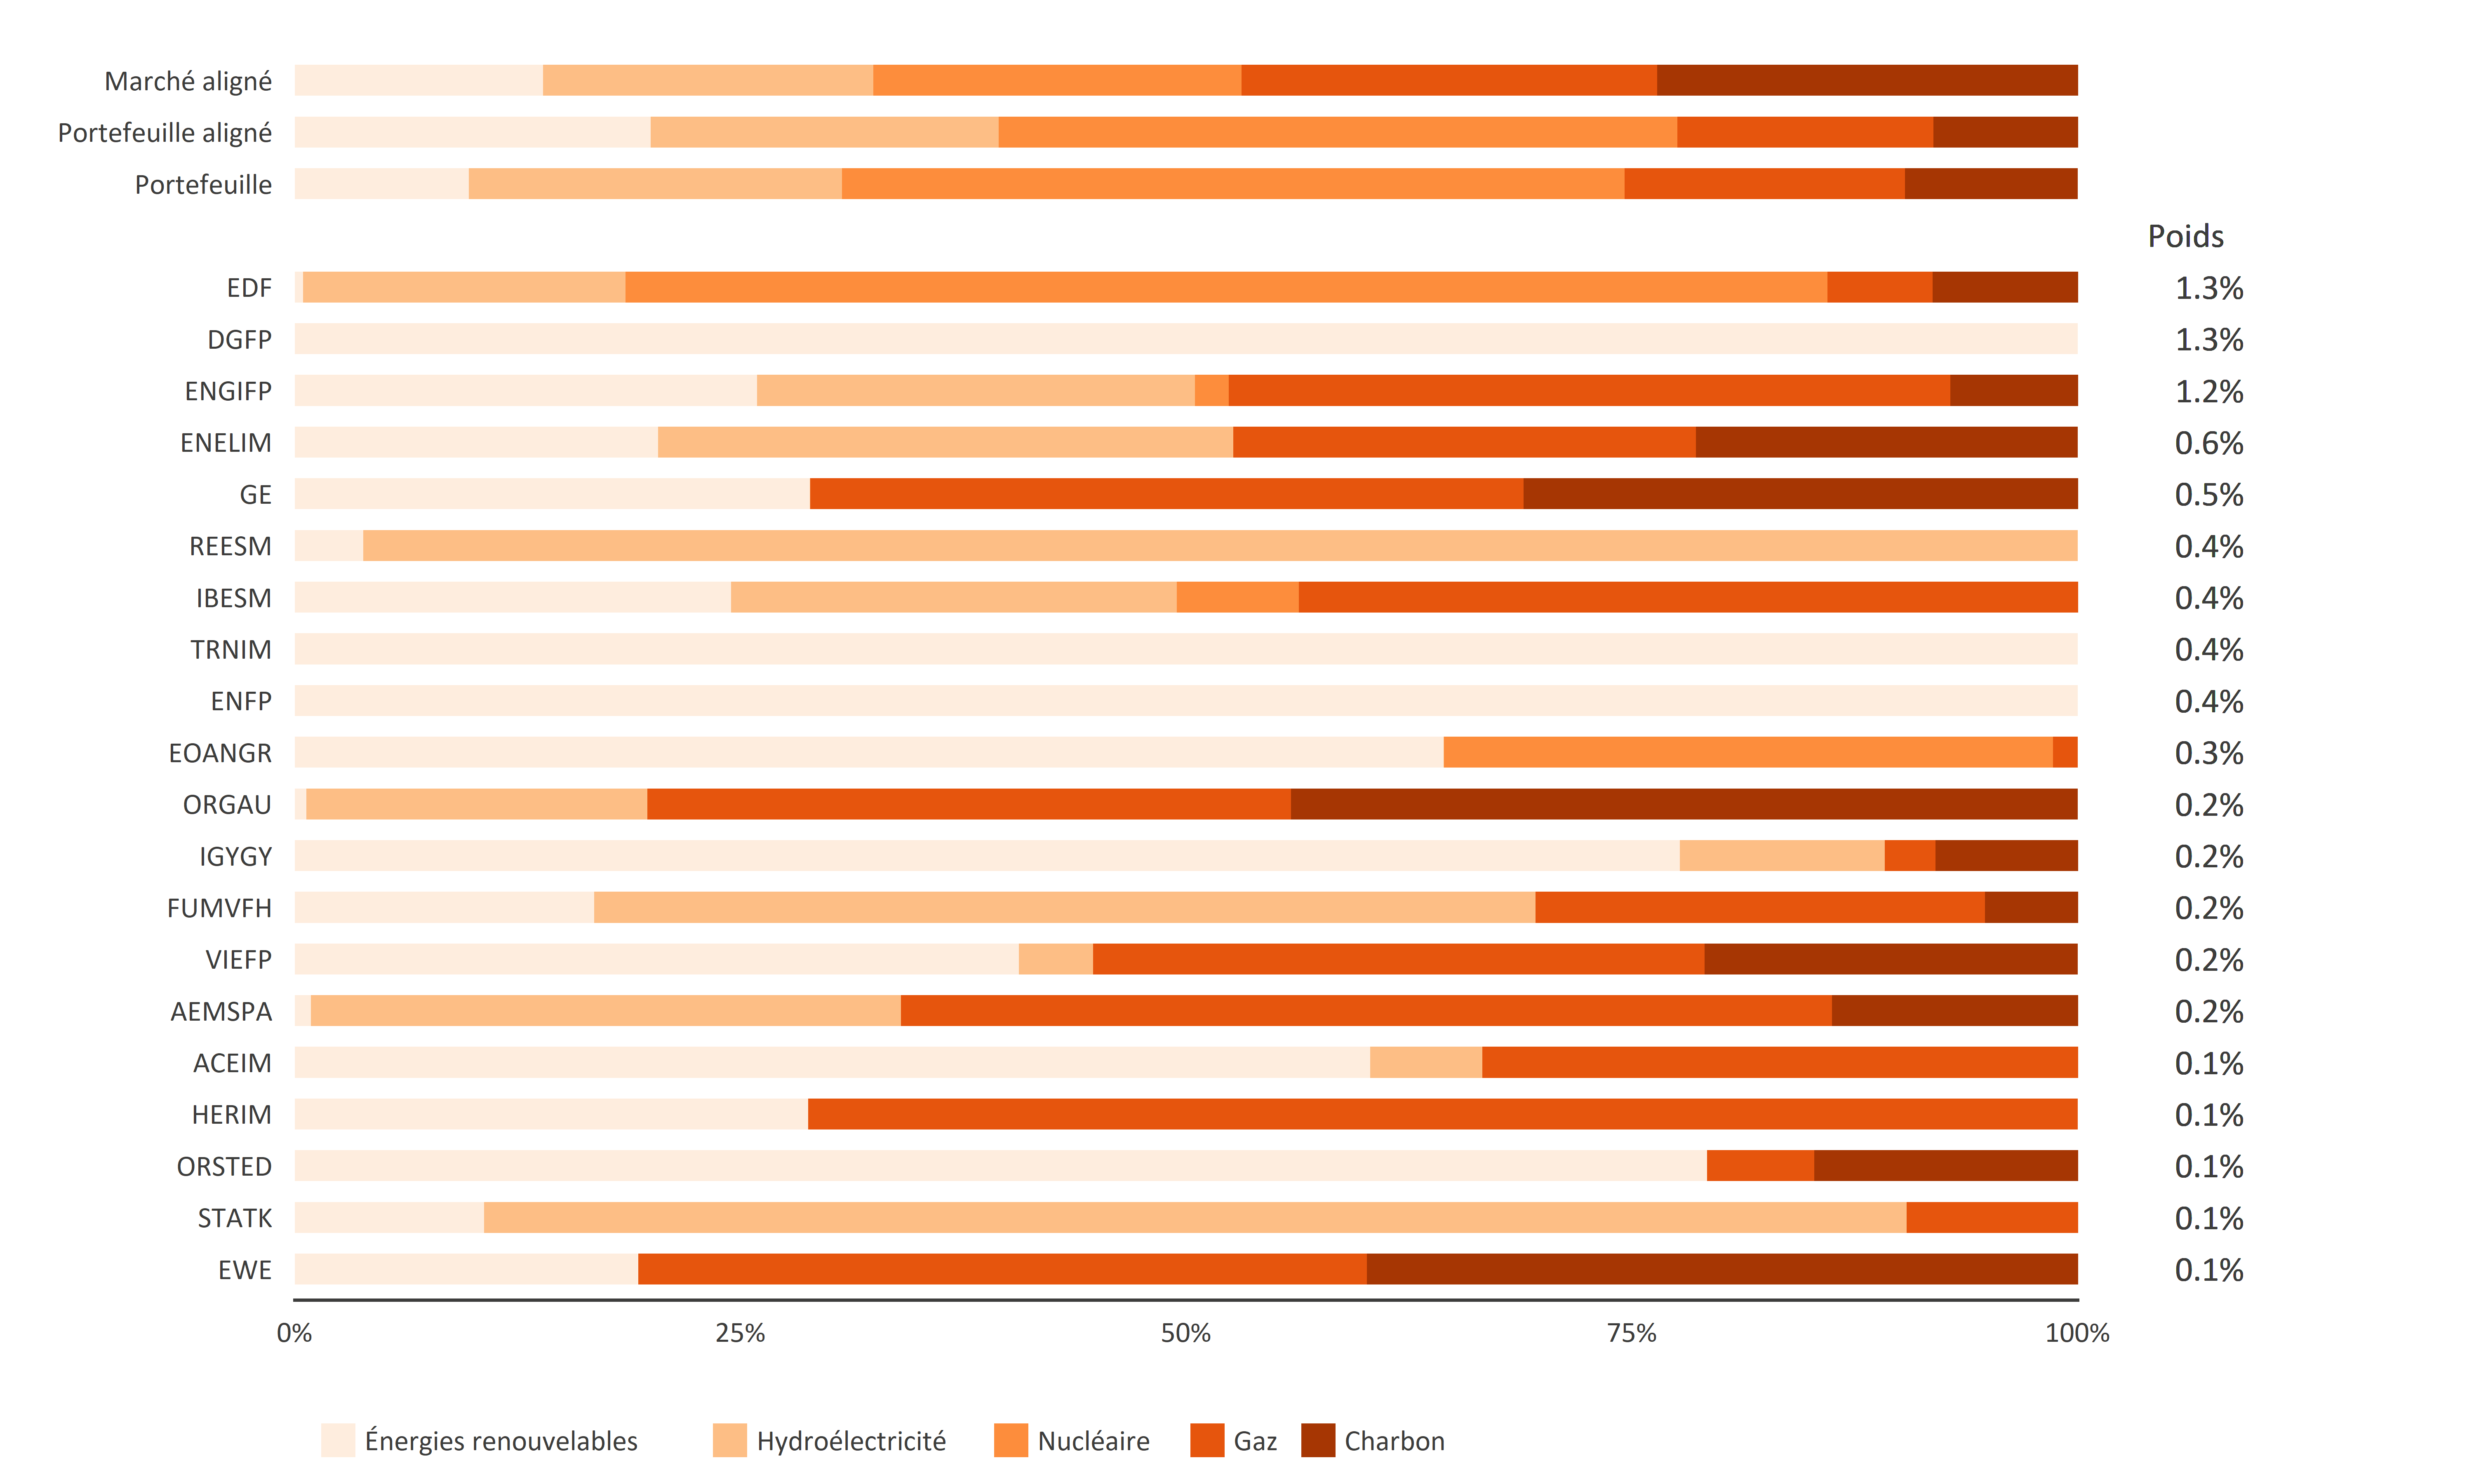
\includegraphics[trim = {0 0cm 0 0},width=1\linewidth]{ReportOutputs/Fig40}
	\end{center}
	%PowerSector_CBE
	%PowerSector_EQS
	\textbf{Technology breakdown of power companies within the equity portfolio}
	\vspace{-.0cm}
	
	\begin{center}
		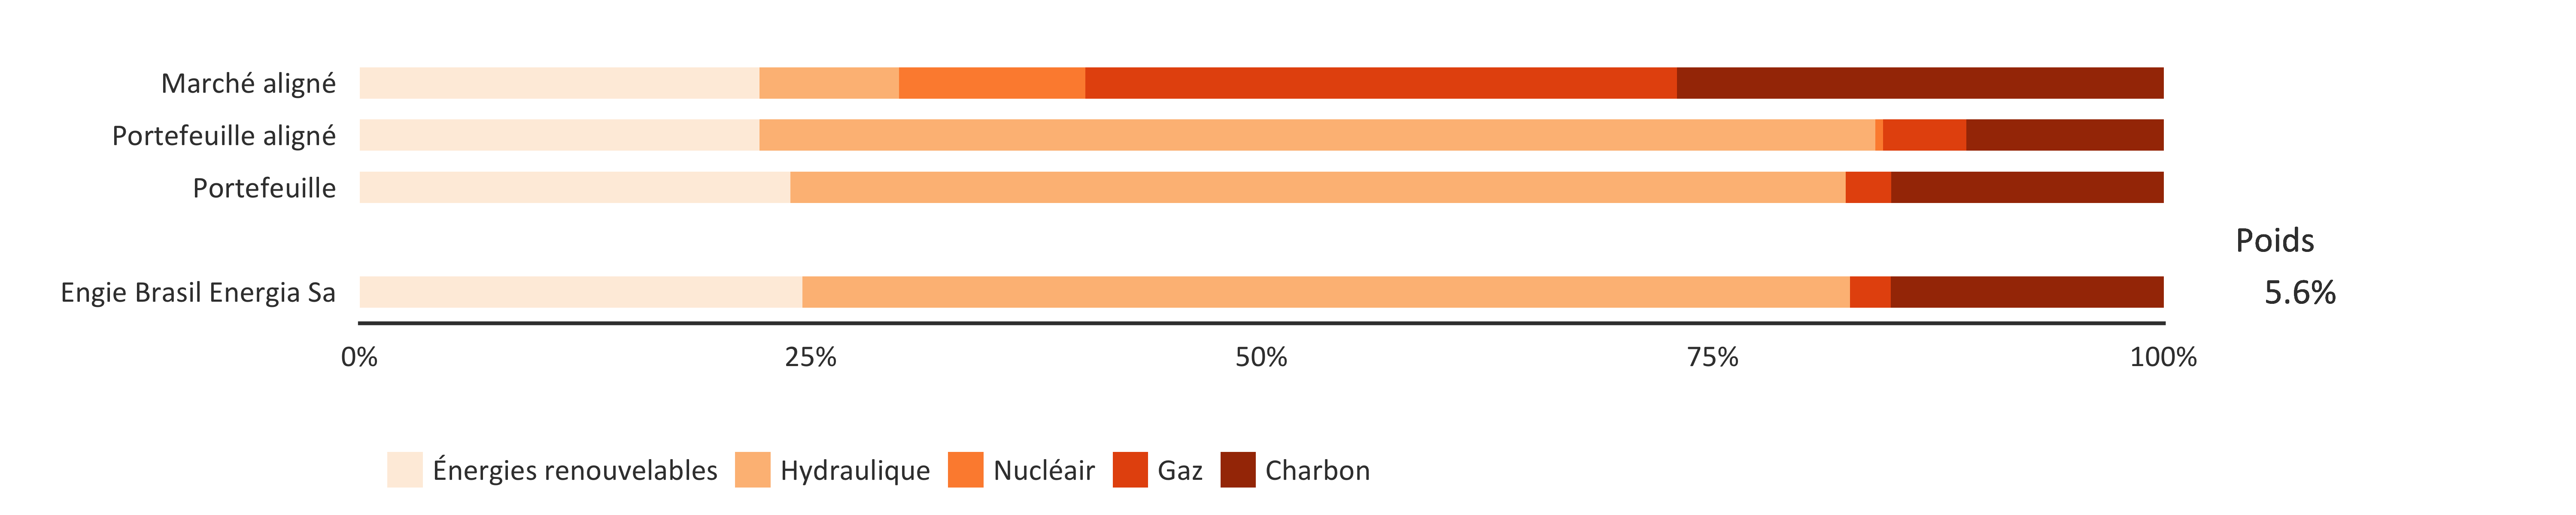
\includegraphics[trim = {0 0cm 0 0},width=1\linewidth]{ReportOutputs/Fig44}
	\end{center}		
	%PowerSector_EQE
	
	%PowerAutoOneSectorS
	%\PageFooterFifth
\PageFooter{5 - COMPANY EXPOSURE}
	
	\newpage
	%PowerSector_ALLE
	%AutoSector_ALLS
	\section*{} % CONTRIBUTIONS OF SECURITIES TO THE RESULTS 
	\HeaderDouble{CONTRIBUTIONS OF SECURITIES TO THE RESULTS}{AUTOMOTIVE}
	%PowerAutoOneSectorE
	
		\textbf{The figures below show the currently planned production mix of engine technologies in Startyear+5 for the largest holdings (by market value) of automobile manufacturers in the corporate bond and equity portfolios.} 
		
		
		The results are shown compared to the portfolio's currently planned production mix, the portfolio's target production mix under the ScenarioValue, an the aligned market's currently planned production mix all as of Startyear+5. The weight is the size of the total investment in each company as a percent of the total value of the relevant portfolio.
		
	
	%AutoSector_CBS
	\textbf{Technology breakdown of automotive companies within the corporate bond portfolio}
	\vspace{-.0cm}
	
	\begin{center}
		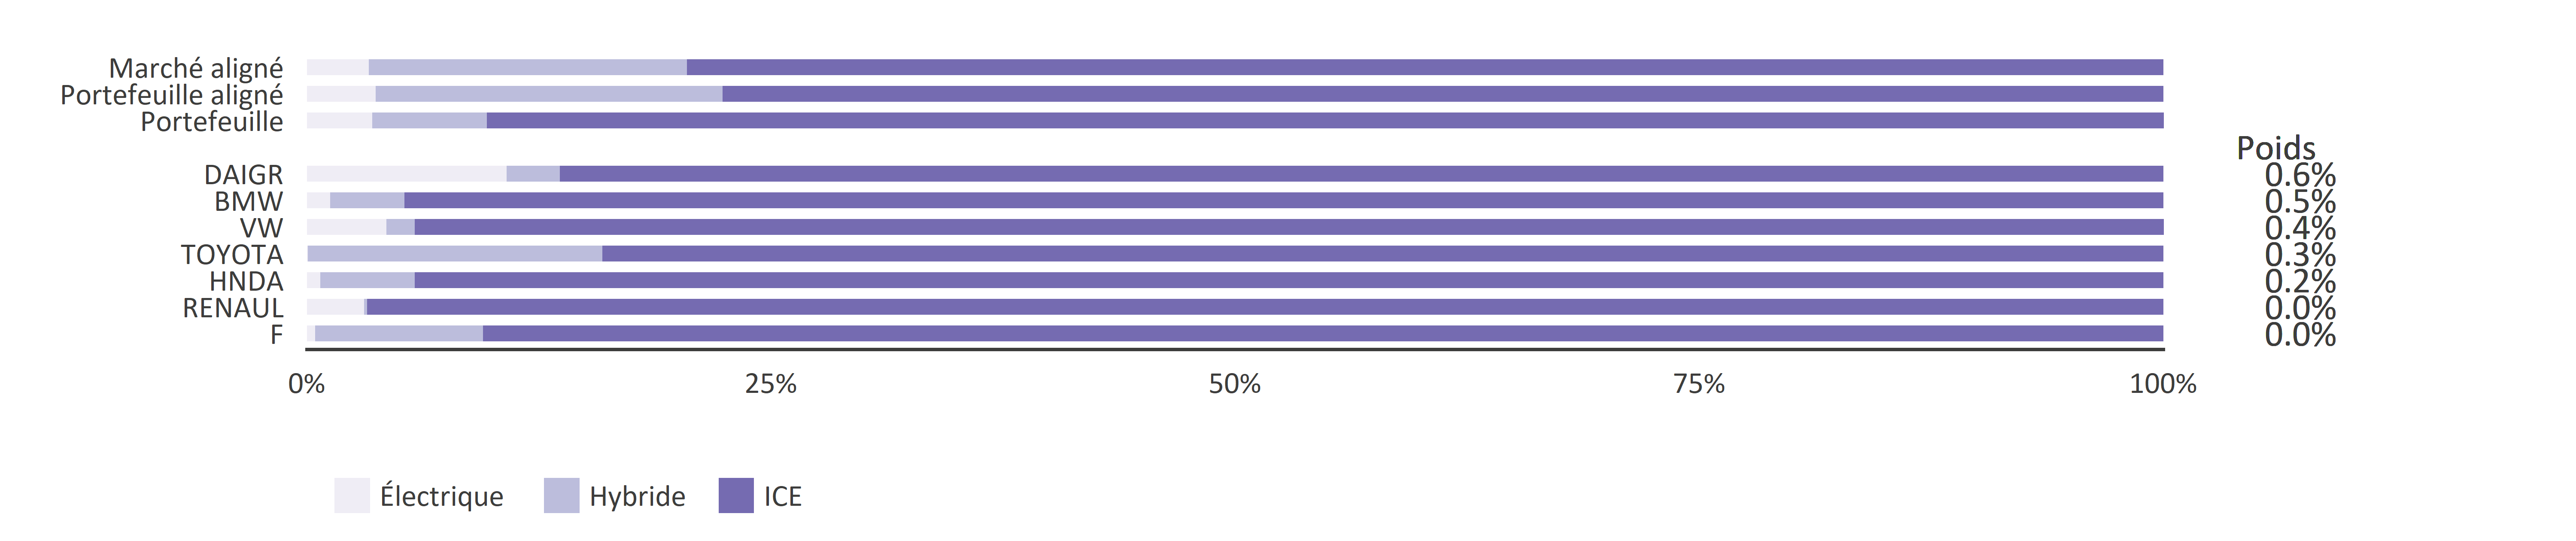
\includegraphics[trim = {0 0cm 0 0},width=1\linewidth]{ReportOutputs/Fig41}
	\end{center}
	%AutoSector_CBE
	
	%AutoSector_EQS
	\textbf{Technology breakdown of automotive companies within the equity portfolio}
	\vspace{-.0cm}
	
	\begin{center}
		
\includegraphics[trim = {0 0cm 0 0},width=1\linewidth]{ReportOutputs/Fig45}
	\end{center}
	%AutoSector_EQE
	
	%\PageFooterFifth
\PageFooter{5 - COMPANY EXPOSURE}

	\newpage
\section*{} % 5th SECTION   
\SectionHeading{SECTION 6:}{BACKGROUND TO THE MODEL}

	\newpage



\section*{} % BACKGROUND TO THE MODEL
\HeaderSingle{CONTEXT}

\begin{multicols}{2}
	
	\textbf{Background. }In June 2017, the G20 Financial Stability Board Task Force on Climate-related Financial Disclosures (TCFD) recommended that financial institutions perform scenario analysis on their portfolios to assess financial risks related to climate change. The TCFD grouped climate-related risks into two categories: physical and transition risks. Transition risks are risks generated by the policy, technology, market, and regulatory changes likely to accompany the transition to a low carbon economy.
		
	\textbf{Goal. }IThe goal of the scenario analysis is to assess investors’ exposure to transition risk, individually and as a whole, based on their estimated current and future exposure to high-carbon and lowcarbon activities. This report provides the results of the analysis for a single portfolio.
		
	
	\textbf{Approach. }The key elements of the analysis are:
	
	\begin{itemize}
		\item{\textit{Current and planned production and investment trends.} Current and planned production (for the fossil fuel and automotive sector) and current installed capacity as well as new capacity additions (for the power sector) for the next 5 years were sourced from commercial business intelligence databases. These data providers collect forward-looking production and capacity data at the physical asset level, including barrels of oil by field, cars by model and factory, and new capacity by power plant. 2Dii maps this data to their immediate owners and parent company to generate a company’s aggregate ‘current production profile’ for each technology. These production plans are linked to the financial securities (equity and corporate bond) issued by the company. The asset-level data used for this analysis was obtained from data providers from December 2018. See the ‘Important Considerations and Limitations’ section at the end of the report for notes on interpreting power sector capacity data.}
		
		\item{\textit{Allocating the production of physical assets to financial assets. }Based on the share of total equity or debt held in a portfolio, the model allocates a portion of each corporate issuer’s current production plans for each technology to the portfolio. Aggregated over all companies to the portfolio level, this is the portfolio’s ‘current production profile’ for a technology. This also defines the investor’s current ‘exposure’ to each technology.}
		
		\item{\textit{From macro-level scenarios to micro-level targets. }To calculate production levels consistent with a climate scenario such as the IEA sustainable development scenario, the model uses a ‘fair share’ principle that applies the changes specified by the scenario for a given technology and region equally across all owners of physical assets in that technology’s sector in the given region. This creates a set of alternative, forwardlooking production and capacity profiles consistent with the scenario for each company and technology. These alternative profiles are then aggregated to the portfolio level to create the portfolio’s ‘target production profile’ under the scenario. This profile is used to determine the investor’s ‘target exposure’ to a technology under the scenario. The ‘target exposure’ does not assume any change in the composition of the portfolio: it models the changes in production and investment plans that are required across the different companies held in the portfolio in order to match the technology deployment described in the scenario.}
		
		\item{\textit{Emissions intensity analysis. }For sectors where there is not sufficient data available either regarding the assets or the scenarios and where there are no commerically suitable replacements, one solution is to analyse required changes in emissions intensity. For these sectors, decarbonisation efforts will be confined to increasing efficiency in production and use, as well as investment in research and development in the next 5-10 years, in order to bring CO$_2$-neutral alternatives to market maturity in the medium term. As a result, both the scenarios and the data are relatively imprecise..}
		
	\end{itemize}
	
		\textbf{Results of the scenario analysis. }The portfolio’s ‘target profile’ under the scenario can be compared to the portfolio’s currently revealed production and investment plans for each technology to derive the exposure to transition risk as well as the extent to which the portfolio is projected to increase or decrease alignment with the SDS over the next 5 years.
\end{multicols}

\PageFooter{7 - BACKGROUND TO THE MODEL}


			
	\newpage
	
	
		
	\section*{} % BACKGROUND TO THE MODEL
	\HeaderSingle{BACKGROUND TO THE MODEL}
	
	\begin{multicols}{2}
		
		
		\textbf{Assessing Alignment with a ScenarioValue Transition Pathway. }This analysis assesses the level of alignment with a ScenarioValue transition pathway, using two references:
		
		\begin{itemize}
			\item{\textit{The portfolio under a ScenarioValue transition.} This is the portfolio's target production profile `under the ScenarioValue': the changes required in the production profile of the companies held in the portfolio, in order to meet the target, based on the above-described methodology. Since the securities held and their weight in the portfolio are identical for the portfolio and its alternative versions, comparing them shows how aligned or misaligned the current production profiles of companies held in the portfolio are with each scenario.}
			
			\item{\textit{The ScenarioValue market. }This is the target production profile of the market under the ScenarioValue. The same principle as described above is applied to an aligned portfolio: the listed equity market as a whole, or the corporate bond market as a whole. Since the securities and their weight in the market portfolio differ from those in the portfolio, this comparison highlights `idiosyncratic' alignment or misalignment. In other words, it shows how the current composition of the portfolio affects the alignment with the different scenarios, when the first reference only stresses the changes requested from the companies.}
		\end{itemize}
		
		
		The alignment or misalignment of a portfolio's production and exposure to each technology relative to a scenario is one way to better understand an investor's exposure to energy transition risk. If policy, technology, market, or regulatory changes occur to bring the global real economy in line with the ScenarioValue, misalignment in a given technology would likely change the financial returns associated with those underlying physical assets. However, this analysis only assesses one dimension of energy transition risks: the assets at risk in the real economy. It does not take into account the financial resilience of the company to those changes and its capacity to adapt, which would require further financial analysis.
		
		\textbf{Scenarios.} This scenario analysis is based on scenarios developed by the IEA. The Beyond 2 degrees scenario (B2DS) focuses on achieving sustainable growth while limiting temperature rise to below 2\degree\ C. The Sustainable Development Scenario (SDS) is a move towards a holistic approach to sustainability rather than focussing solely on climate change. In addition to the SDS, the IEA also defines the New Policies Scenario (NPS) and Current Policies Scenario (CPS): other technology roadmaps that correspond to a 50\% probability of maximum 4\degree C and 6\degree C warming, respectively. The SDS (also referred as the `2\degree\ scenario'), NPS (`4\degree\ scenario'), and CPS (`6\degree\ scenario') all provide forward-looking projections with enough regional detail to perform scenario analysis for 11 technologies in 3 sectors.
		
		The model uses the following indicators from the International Energy Agency scenario against which the portfolio is compared:
		\begin{itemize}
			\item{Electric capacity by fuel expressed in MW (e.g. renewables, coal, gas, oil, hydropower, nuclear);}
			\item{Oil production expressed in barrels of oil / year;}
			\item{Gas production expressed in m\textsuperscript{3} / year;}
			\item{Coal produced expressed in tonnes / year;}
			\item{GHG emissions pathways in a sample of additional sectors (e.g. aviation, shipping, cement, steel).}
		\end{itemize}
		
		 
		\textbf{Asset Level Data.} The Asset Level data is sourced from the following data providers: 
		\begin{itemize}
			\item{GlobalData (Power plant data, including plants classified as active, announced, financed, partially active, permitting, temporarily shutdown, under construction, under rehabilitation and modernization, and Oil and Gas production data and forecasts until Startyear-Startyear+5, as well as coal mining data); }
			\item{WardsAuto (light passenger duty vehicles, including BAU production forecasts Startyear-Startyear+5); }
			\item{Bloomberg (financial data);}
			\item{S\&P Cross-Reference Services (database matching securities to parents);}
			\item{Morningstar (database on funds). }
			
		\end{itemize}
		
		\textbf{Model Parameters.} The scenario analysis presented here reflects a selection of parameter inputs. More details to these parameters and the different implications of the specification of these can be found at www.transitionmonitor.com/backgroundinformation. 
		
		
		
	\end{multicols}
\PageFooter{7 - BACKGROUND TO THE MODEL}
	
	
	\newpage
	
	\section*{} % BACKGROUND TO THE MODEL
	\HeaderDouble{IMPORTANT CONSIDERATIONS AND LIMITATIONS}{WHEN INTERPRETING THESE RESULTS }
	
	\begin{multicols}{2}
		\begin{itemize}
			\item{\textit{Stringency of scenarios.} The use of a given scenario (B2DS, SDS, NPS, CPS) does not constitute an assumption that this scenario is more likely to prevail than others. Similarly, the choice of IEA scenarios should not be interpreted as an endorsement of the underlying assumptions by 2Dii. The IEA historically has assumed significant amounts of nuclear power and carbon capture and storage in their scenarios, an assumption that is debated within the energy-climate scientific community. In addition, the international community has accelerated their global target from the 2\degree C goal to well below 2\degree C and towards 1.5\degree C. It is important to highlight that each investor can and may want to take an individual view on the likely decarbonization scenario that may or may not relate to the scenarios modelled by the International Energy Agency.}
			
			\item{\textit{A snapshot rather than forecasts.} The forward-looking production data is based on current `revealed' plans from companies, and is subject to change. The estimates should thus not be interpreted as forecasts, but rather as the current plans of companies as estimated from various sources of information by industry-specific business intelligence experts. Given the 5 year time horizon, it is likely that these plans will change in some way over time. Similarly, investors are highly likely to alter the composition of their portfolio over time. Corporate bond maturity is usually around 3-7 years. The average holding period of a stock by a fund manager is 20 months on average. However, this analysis seeks to be a point in time assessment of future exposures under current conditions.}
			
			\item{\textit{Power sector projections.} Distinct from the production data for the fossil fuel and automotive sectors, capacity data for the power sector does not include information on planned retirements. It should therefore be interpreted as a measure of currently locked-in capacity and not as a forecast of future capacity. Retirements are not included for several reasons: First, the availability of planned retirement data is highly variable across jurisdictions and regions, to the extent that including no retirement information was deemed more representative of industry capacity than including partial data. Second, in contrast to the fossil fuel sector where oil wells, gas fields, and coal mines cease production when their resource runs out, it is possible for power plants to be announced as retired or even be retired and then resume production. Given the higher level of uncertainty around planned retirements, they are not included in the power sector projections used for this analysis, and capacity projections should thus be interpreted as the potential maximum `lock-in' from current infrastructure. For technologies projected to decline under the ScenarioValue, the gap between current capacity projections and capacity consistent with the ScenarioValue should be seen as an estimate of the capacity that would need to be retired to be in alignment with the ScenarioValue.} 
			
			\item{\textit{Ability to capture SRI strategies. }The model takes a diversified `market portfolio' as a basis, focusing on key technologies reflected in the IEA roadmaps. By extension, thematic portfolios invested in breakthrough technologies and / or SRI portfolios with a range of environmental, social, and governmental considerations may not value these elements.}
		\end{itemize}
		
		
	\end{multicols}
\PageFooter{7 - BACKGROUND TO THE MODEL}

	\newpage		
	
	\section*{} % CONTEXT p8
	\HeaderSingle{TRANSITION RISK FOR INVESTORS}
	\begin{multicols}{2}
		\textbf{What are transition risks?} Transition risks can be broadly defined as economic and financial risks associated with the transition to a low-carbon economy. The international community has defined a mandate to limit the man-made contribution to global warming to well below 2\degree C above pre-industrial levels. According to best available science, achieving this objective requires decarbonizing the economy in the course of this century. This decarbonization is set to have significant implications for high-carbon sectors, most prominent among which are the fossil fuel, power, and transport sectors, contributing the majority of global anthropogenic GHG emissions. 
		
		As the economy decarbonizes, companies that fail to properly anticipate this transition are set to be exposed to economic risks. Companies well-prepared for this transition in turn are set to capitalize from this economic opportunity. Similarly, economic risks may translate into financial risks in financial markets if these risks are not properly anticipated by financial market actors. 
		
		Crucially, the transition to a low-carbon economy is set to already have dramatic impacts in the short- and medium-term. By 2040, in only 22 years, global coal production is set to decline by 46\%, with a more accelerated decline expected in developed markets. Global coal power capacity in turn is similarly set to decline by 41\%. The production of gasoline and diesel vehicles (internal combustion engine or ICE vehicles) is set to decline by 21\%. This decline in high-carbon activity in turn will be accompanied by the commensurate deployment and growth of new technologies. Renewable power capacity and electric vehicle production in turn is set to nearly quadruple in volume by 2040. 
		
		Scenario analysis can help financial institutions assess and ultimately manage the risks and opportunities associated with the transition. In recognition of these risks, scenario analysis has been applied to date by hundreds of financial institutions as well as financial supervisors. It forms the basis of the recommendations of the FSB TCFD. The TCFD notes that ``forward-looking assessments of climate-related issues is important for investors and other stakeholders in understanding how vulnerable individual organizations are to transition and physical risks and how such vulnerabilities are or would be addressed. As a result, the Task Force believes that organizations should use scenario analysis to assess potential business, strategic, and financial implications of climate-related risks and opportunities and disclose those, as appropriate, in their annual financial filings" (TCFD Final Report, p. 33). 
		
		To clarify its scenario analysis recommendation, the Task Force explains, ``A key type of transition risk scenario is a so-called 2\degree C scenario, which lays out a pathway and an emissions trajectory consistent with holding the increase in the global average temperature to 2\degree C above pre-industrial levels" (TCFD Final Report, p. 35).
		
		It is this premise that forms the basis of this report, highlighting for the portfolio the current exposure to transition risks in the fossil fuel, power, and automotive sectors, the trends in the portfolio over time in these sectors relative to the 2\degree C scenario, and the expected future exposure on the basis of these trends. While these sectors do not represent all high-carbon activities and sectors, they account for both the largest share in a typical portfolio and the most significant contribution to climate change currently, as well as benefiting from well-developed scenario pathways.
		
		The report does not provide specific estimates as to the potential loss in value that may be realised in the portfolio should these risks materialize, which is obviously associated with significant uncertainty and myriad modelling assumptions. For any individual security, the potential loss may range from 0 to 100\% and may even be associated with positive returns, depending on the adaptive capacity of the company, the anticipation of the trend by financial markets, and the nature of a potential repricing. It is the proper anticipation of these risks that minimizes the loss that this report seeks to contribute to. 
		
		
		
	\end{multicols}
	
	\textbf{Volume change by 2023 and 2040 under the 450S Scenario.}
	\begin{center}
		{\setlength{\tabcolsep}{10pt} % Default value: 6pt
			\renewcommand{\arraystretch}{1} % Default value: 1
			\begin{tabular}{ p{.24\linewidth}| P{.24\linewidth}| P{.24\linewidth}}
				\hline
				\textbf{Technology} & \textbf{Total Volume Change by 2023} & \textbf{Total Volume Change by 2040} \\ 
				\hline
				Renewable Power & 69\% \nearr{ColGreen} & 354\% \uparr{ColGreen}\\
				Hydro Power & 13\% \nearr{ColGreen} & 59\% \nearr{ColGreen}\\
				Nuclear Power & 17\% \nearr{ColGreen} & 89\% \nearr{ColGreen}\\
				Gas Power & 8\% \nearr{ColGreen} & 31\% \nearr{ColGreen}\\
				Coal Power & -3\% \searr{ColRed} & -41\% \searr{ColRed}\\				
				\hline
				Oil Production & -2\% \searr{ColRed} & -23\% \searr{ColRed}\\
				Gas Production & 5\% \nearr{ColGreen} & 8\% \nearr{ColGreen}\\
				Coal Production & -11\% \searr{ColRed}& -46\% \searr{ColRed}\\ 
				\hline
				ICE Production & -9\% \searr{ColRed} & -21\% \searr{ColRed}\\
				Hybrid Production & 97\% \uparr{ColGreen} & 440\% \uparr{ColGreen}\\
				Electric Production & 105\% \uparr{ColGreen} & 352\% \uparr{ColGreen}\\
				\hline
			\end{tabular}
		}
	\end{center}
	
	\textit{\small Source: IEA World Energy Outlook 2016
	}

\PageFooter{7 - BACKGROUND TO THE MODEL}

	\newpage
	\section*{} % UNDERSTANDING THE POWER SECTOR
	\HeaderSingle{UNDERSTANDING THE POWER SECTOR}	
	
	
	\begin{multicols}{2}
		
		The analysis for the power portfolio builds on the forward-looking projections of capacity additions by fuel over the next 5 years, as sourced from business intelligence data provider GlobalData. The five year time horizon is a function of the typical investment planning horizon of power capacity additions, recognizing that planning horizons for specific investments may be either longer or shorter. More long-term analysis would thus fail to identify significant further additions currently in the planning pipeline of companies. Excluded from the company information charts are the planned power capacity additions by companies outside of the power sector (e.g. IT companies building wind parks to power their data centers). The evolution of the portfolio is based on the planned capacity additions by the companies behind the securities in the portfolio, weighted by their relative weight in the portfolio. 
		
		It is important to note that data on announced or otherwise officially planned retirements of power assets is not considered in the analysis presented here. This is intentional, given both a dearth of related data, as well as the desire to show the required retirements. For technologies projected to decline under the ScenarioValue, the gap between current capacity projections and capacity consistent with the ScenarioValue should be seen as an estimate of the capacity that would need to be retired to be in alignment with the ScenarioValue. 
		
		As outlined above, the scenarios are based on the global trends, scaled to the portfolio based on the `fair share' approach, where the trend in the macro scenario is translated into a micro target based on the market share of the portfolio. For the power sector, this approach may of course fail to capture changes in market share across asset classes and actors, notably with the rise of household renewable power capacity (e.g. rooftop solar), set to change the power market. While this trend implies that in practice companies are likely to lose market share, this trend is intentionally not internalized in the analysis, in order to document the potential loss of market share under a ScenarioValue - and by extension the potential accumulating transition risk.
		
		In a 2\degree C or below scenario, the power sector will decarbonize over the long-term in a shift from fossil fuel-based to renewable energy production. The International Energy Agency (IEA) says that in a 2\degree C scenario:
		
		``Electricity supply worldwide is set to diversify and decarbonise, with low-carbon generation overtaking coal before 2020. Coal-fired power's share of generation is projected to fall from above 40\% now to 28\% in 2040. By then, wind, solar and bioenergy-based renewables combined increase their market share from 6\% to 20\%" (IEA World Energy Outlook 2016, p. 241).
		
		The mix of technologies will vary greatly based on the scenario. Coal-based power generation will increase under current trends but decreases in a 2\degree C scenario. Wind and solar would grow more rapidly in a 2\degree C Scenario.
		
		Equity and corporate bond investors are exposed to these trends through the financial instruments issued by power companies. An estimated 28\% of power generation assets are owned by publicly traded companies and 19\% of assets are owned by listed state entities, for example municipal bond issuers (see figure below).
	\end{multicols}
	
	\begin{multicols}{2}
		
		\vspace{-.2cm}
		\textbf{Power generation mix under IEA business as usual and 2DS scenarios for selected technologies}
		
		
		
		
		\adjincludegraphics[width = .95\linewidth,trim={0cm 0cm 0cm .5cm},clip]{ReportGraphics/PowerLine.png}
		
		\textit{\small Source: IEA World Energy Outlook 2016
		}
		
		\textbf{Ownership of global power generation assets}
		\newline
		
		\adjincludegraphics[width = .8\linewidth,trim={0cm 0cm 0cm 0.5cm},clip]{ReportGraphics/PowerPie.png}
		
		\textit{\small Source: IEA analysis and 2Dii, based on Platts, Bloomberg Professional service, Bloomberg New Energy Finance and national sources
		}
		
	\end{multicols}

\PageFooter{7 - BACKGROUND TO THE MODEL}		
		
		
	\newpage
	\section*{} % EMISSIONS INTENSITY ANALYSIS
	\HeaderSingle{EMISSIONS INTENSITY ANALYSIS}
	
		\begin{multicols}{2}
			
			
			\textbf{Methodology}
			
			For the emissions intensity analysis an emission factor for each plant is calculated in units per production. This is then aggregated to the portfolio by weighting by the weight of the company within the portfolio. The scenario data is then scaled to this starting point and the trajectory for emissions reduction is shown for the next five years. 
			
			These results can serve as a starting point for discussions with steel, cement, aviation and shipping companies regarding their strategies for achieving the trajectory for each sector. 
			
				
			\textbf{Scenarios} 
			
			The emissions intensity reduction pathway is based on the scenarios presented in the Energy Technology Perspectives 2017. The expected production and emissions for the steel, cement and aviation sectors are provided at a regional level. The pathways presented in this sector follow the 2\degree\ C scenario. The shipping sector does not have sufficient data to complete this, and therefore the portfolio is compared to market.
			
			
			\textbf{Steel} 
			
			After chemicals, steel production is the second largest energy consumer among industrial sectors and the most carbon-intensive sector. The deployment of 	electric arc furnaces is key to reducing emissions (even if this technology remains carbon-emitting). The calculation of an emissions factor for each steel plant is based on the technology deloyed, the fuel used, and the regional factors for emissions from the electricity grid and fuel consumption as relevant. Additionally this is then multiplied by the plant capacity and a regionally selected capacity factor. These factors are sourced from the OECD data bases and the World Steel Association.  
			
 			\textbf{Cement}
 			
			Cement production is another high emitting sector, with concrete production expected to account for 5\% of the world's man made emissions (Cement Sustainability Initiative). This comes primarily in the production from three sources, the calcination process, thermal energy use and electricity use. The emissions factor is calculated from regional factors applied to each plant. The majority of the data for this comes from the Cement Sustainability Initiative. 
			
			\textbf{Aviation}
			
			To estimate the current CO\textsubscript{2} emissions from aircraft fleets assumptions regarding aircraft utilization rates were made. The emissions have been estimated for each company on a per passenger kilometer basis; an equivalent for aircraft used for freight only has been calculated. There is a high level of uncertainty in this methodology.
			
			\textbf{Shipping}
			
			The best practice for shipping sustainability assessments is the  Carbon Efficiency Level, developed by Carbon War Room and Rightship. Each vessel is rated from A to G, where A is the most efficient ships in each ship category (eg. oil tanker, cargo, etc.), allowing for a common point of comparison. The ranking is dynamically calculated to account for annual improvements in efficiency and variations in the mean, so that ``A" ships always represent the top 10\% (measured in terms of CO\textsubscript{2} intensity). As there is no scenario data available the shipping results for the portfolio are compared to the market. 
			
			
			
			
			
		\end{multicols}	
\PageFooter{7 - BACKGROUND TO THE MODEL}


	
	\newpage
	%WWFSpecificIncludeE
	\section*{} % NOTES AND DISCLAIMER
	\HeaderSingle{NOTES}
	
	\begin{multicols}{2}
		The data and scenario sources for this analysis are provided below. 
		
		\textbf{Published Research}
		
		The methodology behind this scenario analysis, the accounting rules applied, and further information to the scenarios and data can be found in the following published research papers. 
		
		Accounting Principles: http://www.mdpi.com/2071-1050/ 10/2/328 
		
		Scenario Work: http://et-risk.eu/toolbox/ scenarios/ 
		
		Asset Level Data Analysis: http://2degrees-investing.org/ IMG/pdf/assetdata\_v0.pdf
		
		\textbf{Sources for the data and scenario analysis}
		
		Automobile data are from July 2017 and is provided by WardsAuto / AutoForecastSolutions. Power data is from July 2017 and is provided by GlobalData. Oil, gas and coal production data is from July 2017 and is provided by GlobalData. When linking asset data with companies, the data is used by the data providers mentioned above and, where possible, enriched with company data from Bloomberg. All financial data, as well as identification numbers for linking company data with financial instruments, come from Bloomberg. 
		
		The decarbonization pathways for other sectors comes from the Science-Based Targets Initiative, which bases its methodology on the IEA scenarios. The scenarios for the energy and power sector come from the IEA's World Energy Outlook 2016. Because this report does not include scenario information for the automotive sector, the related data is taken from the sister report of the World Energy Outlook, the Energy Technology Perspective report. Benchmarks for the electricity sector are determined regionally and applied in relation to the regional exposure data and then aggregated, weighted according to the regional exposure of the portfolio. All other results are global.
		
		\textbf{Sources}
		
		Cement Sustainability Initiative (2018) https://www.wbcsdcement. org/index.php/key-issues/climate-protection
		
		Energy Technology Perspectives 2017 (2018) https://www.iea.org /etp/
		
		IPCC (2018) https://www.ipcc.ch/report/ar5/
		
		FSB (2018) https://www.fsb-tcfd.org/publications/final-recommendations-report/
		
		WoodMackenzie (2018) https://www.woodmac.com/news/ editorial/carbon-intensity-not-all-assets-are-created-equal/ 
		
		World Energy Outlook 2017 (2018) https://www.iea.org/weo2017/
	
	\end{multicols}
	
\PageFooter{7 - BACKGROUND TO THE MODEL}	
	
	\newpage

	
\end{document} 

